% $Author: --- $
% $Date: 2010-05-13 23:11:04 +0200 (Thu, 13 May 2010) $
% $Revision: 32942 $

% HISTORY:
% 2012-11-11: Stephane is doing a pass after Andre's one.

%=================================================================
\ifx\wholebook\relax\else
% --------------------------------------------
% Lulu:
	\documentclass[a4paper,10pt,twoside]{book}
	\usepackage[
		papersize={6.13in,9.21in},
		hmargin={.75in,.75in},
		vmargin={.75in,1in},
		ignoreheadfoot
	]{geometry}
	% $Author$
% $Date$
% $Revision$

% HISTORY:
% 2006-10-31 - Oscar code macros
% ...

%=============================================================
% NB: documentclass must be set in main document.
% Allows book to be generated in multiple formats.
%=============================================================
%:Packages
\usepackage[T1]{fontenc}  %%%%%% really important to get the code directly in the text!
\usepackage{lmodern}
%\usepackage[scaled=0.85]{bookmanx} % needs another scale factor if used with \renewcommand{\sfdefault}{cmbr}
\usepackage{palatino}
\usepackage[scaled=0.85]{helvet}
\usepackage[protrusion,expansion=false]{microtype}
\usepackage{graphicx}
\usepackage{theorem}
\usepackage[english]{babel}
% ON: pdfsync breaks the use of p{width} for tabular columns!
\ifdefined\usepdfsync\usepackage{pdfsync}\fi % Requires texlive 2007
%=============================================================
%:More packages
%Stef should check which ones are used!
%\usepackage{picinpar}
%\usepackage{layout}
%\usepackage{color}
%\usepackage{enum}
%\usepackage{a4wide}
% \usepackage{fancyhdr}
\usepackage{ifthen}
\usepackage{float}
\usepackage{longtable}
\usepackage{makeidx}
\usepackage[nottoc]{tocbibind}
\usepackage{multicol}
\usepackage{booktabs}	% book-style tables
\usepackage{topcapt}	% enables \topcaption
\usepackage{multirow}
\usepackage{tabularx}
%\usepackage[bottom]{footmisc}
\usepackage{xspace}
\usepackage{alltt}
\usepackage{amssymb,textcomp}
\usepackage[usenames,dvipsnames]{color}
%\usepackage{colortbl}
\usepackage[hang]{subfigure}\makeatletter\def\p@subfigure{\thefigure\,}\makeatother
\usepackage{rotating}
\usepackage{enumitem}	% apb: allows more control over tags in enumerations
\usepackage{verbatim}     % for comment environment
\usepackage{varioref}	% for page references that work
\labelformat{footnote}{\thechapter--#1} % to distinguish citations from jurabib
\usepackage{needspace}
\usepackage{isodateo} % enable \isodate
\usepackage[newparttoc,pagestyles]{titlesec}
\usepackage{titletoc}
\usepackage{wrapfig}

\usepackage[
	super,
	citefull=first,
	authorformat={allreversed,and},
	titleformat={commasep,italic}
]{jurabib} % citations as footnotes
\usepackage[
	colorlinks=true,
	linkcolor=black,
	urlcolor=black,
	citecolor=black
]{hyperref}   % should come last
%=============================================================
%:PDF version
\pdfminorversion=3 % Set PDF to 1.3 for Lulu
%=============================================================
%:URL style
\makeatletter
\def\url@leostyle{%
  \@ifundefined{selectfont}{\def\UrlFont{\sf}}{\def\UrlFont{\sffamily}}}
\makeatother
% Now actually use the newly defined style.
\urlstyle{leo}
%=============================================================
%:Booleans
\newboolean{lulu}
\setboolean{lulu}{false}
\newcommand{\ifluluelse}[2]{\ifthenelse{\boolean{lulu}}{#1}{#2}}
%=============================================================
%:Names
\newcommand{\SUnit}{SUnit\xspace}
\newcommand{\sunit}{SUnit\xspace}
\newcommand{\xUnit}{$x$Unit\xspace}
\newcommand{\JUnit}{JUnit\xspace}
\newcommand{\st}{Smalltalk\xspace}
\newcommand{\pharo}{Pharo\xspace} % Use this, not \Pharo
%\newcommand{\sqmap}{SqueakMap\xspace}
\newcommand{\squeak}{Squeak\xspace} % use this, not \Squeak or \sq
\newcommand{\sqsrc}{SqueakSource\xspace}
\newcommand{\sbe}{\url{http://SqueakByExample.org}\xspace}
\newcommand{\pharoweb}{\url{http://pharo-project.org}\xspace}
\newcommand{\pbe}{\url{http://PharoByExample.org}\xspace}
\newcommand{\sba}{\url{http://SquareBracketAssociates.org}\xspace}
\newcommand{\bam}{\lct{Bounc\-ing\-Atoms\-Morph}\xspace}
%=============================================================
%:Markup macros for proof-reading
\usepackage[normalem]{ulem} % for \sout
\usepackage{xcolor}
\newcommand{\ra}{$\rightarrow$}
\newcommand{\ugh}[1]{\textcolor{red}{\uwave{#1}}} % please rephrase
\newcommand{\ins}[1]{\textcolor{blue}{\uline{#1}}} % please insert
\newcommand{\del}[1]{\textcolor{red}{\sout{#1}}} % please delete
\newcommand{\chg}[2]{\textcolor{red}{\sout{#1}}{\ra}\textcolor{blue}{\uline{#2}}} % please change
%=============================================================
%:Editorial comment macros
%\newcommand{\nnbb}[2]{
%    % \fbox{\bfseries\sffamily\scriptsize#1}
%    \fcolorbox{gray}{yellow}{\bfseries\sffamily\scriptsize#1}
%    {\sf\small$\blacktriangleright$\textit{#2}$\blacktriangleleft$}
%   }
\newcommand{\yellowbox}[1]{\fcolorbox{gray}{yellow}{\bfseries\sffamily\scriptsize#1}}
\newcommand{\triangles}[1]{{\sf\small$\blacktriangleright$\textit{#1}$\blacktriangleleft$}}
\newcommand{\nnbb}[2]{\yellowbox{#1} \triangles{#2}}
\newcommand{\fix}{\yellowbox{FIX!}}
\newcommand{\here}{\yellowbox{CONTINUE HERE!}}
% editor macros
\newcommand{\apl}[1]{\nnbb{Alain}{#1}} % Alain
\newcommand{\ab}[1]{\nnbb{Andrew}{#1}} % Black
\newcommand{\sd}[1]{\nnbb{St\'{e}f}{#1}} % Ducasse
\newcommand{\gl}[1]{\nnbb{Guillaume}{#1}} % Ducasse
\newcommand{\cd}[1]{\nnbb{Christophe}{#1}} % Ducasse
\newcommand{\sig}[1]{\nnbb{Igor}{#1}} % Igor
\newcommand{\dc}[1]{\nnbb{DamienC}{#1}} % Ducasse
\newcommand{\md}[1]{\nnbb{Marcus}{#1}} % Denker
\newcommand{\on}[1]{\nnbb{Oscar}{#1}} % Nierstrasz
\newcommand{\damien}[1]{\nnbb{Damien}{#1}} % Pollet
\newcommand{\lr}[1]{\nnbb{Lukas}{#1}} % Renggli
\newcommand{\orla}[1]{\nnbb{Orla}{#1}} % Greevy
\newcommand{\alex}[1]{\nnbb{Alex}{#1}} % Bergel
\newcommand{\alx}[1]{\nnbb{Alex}{#1}} % Bergel
\newcommand{\dr}[1]{\nnbb{David}{#1}} % Roethlisberger
\newcommand{\ja}[1]{\nnbb{Jannik}{#1}} % Laval
\newcommand{\cb}[1]{\nnbb{Camillo}{#1}} % Bruni
\newcommand{\jr}[1]{\nnbb{Jorge}{#1}} % Ressia
\newcommand{\jb}[1]{\nnbb{JB}{#1}} % JB
\newcommand{\jp}[1]{\nnbb{Javier}{#1}} % Pimas
\newcommand{\fp}[1]{\nnbb{Fabrizio}{#1}} % Perin
\newcommand{\michael}[1]{\nnbb{Michael}{#1}} % Davies
\newcommand{\ew}[1]{\nnbb{Erwann}{#1}} % Wernli
\newcommand{\mb}[1]{\nnbb{Martial}{#1}} % Boniou
\newcommand{\hw}[1]{\nnbb{Hernan}{#1}} % Wilkinson
\newcommand{\ben}[1]{\nnbb{Benjamin}{#1}} % Benjamin Van Ryseghem
\newcommand{\hjo}[1]{\nnbb{HwaJong}{#1}} % HwaJong Oh aka daliot
\newcommand{\ml}[1]{\nnbb{Max}{#1}} % Max Leske
\newcommand{\mmp}[1]{\nnbb{Mariano}{#1}} % Mariano Martinez Peck
\newcommand{\luc}[1]{\nnbb{Luc}{#1}} % Luc Fabresse
\newcommand{\dkl}[1]{\nnbb{Daniel}{#1}} % Daniel Lyons
\newcommand{\vu}[1]{\nnbb{Veronica}{#1}} % Veronica Uquillas Gomez
\newcommand{\martin}[1]{\nnbb{Martin}{#1}} % Martin Dias
\newcommand{\vp}[1]{\nnbb{Vanessa}{#1}} % Vanessa Pena
\newcommand{\gp}[1]{\nnbb{Guille}{#1}} % Guillermo Polito

%=============================================================
%:Abbreviation macros
\newcommand{\ie}{\emph{i.e.},\xspace}
\newcommand{\eg}{\emph{e.g.},\xspace}
\newcommand{\etc}{etc.\xspace}
%=============================================================
%:Cross reference macros
\newcommand{\charef}[1]{Chapter~\ref{cha:#1}\xspace}
\newcommand{\secref}[1]{Section~\ref{sec:#1}\xspace}
\newcommand{\figref}[1]{Figure~\ref{fig:#1}\xspace}
\newcommand{\Figref}[1]{Figure~\ref{fig:#1}\xspace}
\newcommand{\appref}[1]{Appendix~\ref{app:#1}\xspace}
\newcommand{\tabref}[1]{Table~\ref{tab:#1}\xspace}
\newcommand{\faqref}[1]{FAQ~\ref{faq:#1}, p.~\pageref{faq:#1}\xspace}
% APB: I removed trailing \xspace commands from these macros because
% \xspace mostly doesn't work.  If you want a space after your
% references, type one!
% ON: xspace has always worked just fine for me!  Please leave them in.
%
\newcommand{\ruleref}[1]{\ref{rule:#1}\xspace}
%
\newcommand{\egref}[1]{example~\ref{eg:#1}\xspace}
\newcommand{\Egref}[1]{Example~\ref{eg:#1}\xspace}
%
\newcommand{\scrref}[1]{script~\ref{scr:#1}\xspace}
\newcommand{\Scrref}[1]{Script~\ref{scr:#1}\xspace}
\newcommand{\tscrref}[1]{the script~\ref{scr:#1}\xspace}
\newcommand{\Tscrref}[1]{The script~\ref{scr:#1}\xspace}
%
\newcommand{\mthref}[1]{method~\ref{mth:#1}\xspace}
\newcommand{\mthsref}[1]{methods~\ref{mth:#1}\xspace}
\newcommand{\Mthref}[1]{Method~\ref{mth:#1}\xspace}
\newcommand{\tmthref}[1]{the method~\ref{mth:#1}\xspace}
\newcommand{\Tmthref}[1]{The method~\ref{mth:#1}\xspace}
%
\newcommand{\clsref}[1]{class~\ref{cls:#1}\xspace}
\newcommand{\tclsref}[1]{the class~\ref{cls:#1}\xspace}
\newcommand{\Tclsref}[1]{The class~\ref{cls:#1}\xspace}

\newcommand{\chalabel}[1]{\label{cha:#1}}
\newcommand{\seclabel}[1]{\label{sec:#1}}
\newcommand{\figlabel}[1]{\label{fig:#1}}
\newcommand{\tablabel}[1]{\label{tab:#1}}
\newcommand{\rulelabel}[1]{\label{rule:#1}}
\newcommand{\eglabel}[1]{\label{eg:#1}}
\newcommand{\scrlabel}[1]{\label{scr:#1}}
\newcommand{\mthlabel}[1]{\label{mth:#1}}
\newcommand{\clslabel}[1]{\label{cls:#1}}
\newcommand{\faqlabel}[1]{\label{faq:#1}}
%=============================================================
%:Menu item macro
% for menu items, so we can change our minds on how to print them! (apb)
\definecolor{lightgray}{gray}{0.89}
\newcommand{\menu}[1]{{%
	\setlength{\fboxsep}{0pt}%
	\colorbox{lightgray}{{{\upshape\sffamily\strut \,#1\,}}}}}
\newcommand{\link}[1]{{%
	\fontfamily{lmr}\selectfont
 	\upshape{\sffamily \underline{#1}}}}
% For submenu items:
\newcommand{\go}{\,$\triangleright$\,}
% \newcommand{\go}{\,$\blacktriangleright$\,}
% For keyboard shortcuts:
%\newcommand{\short}[1]{\mbox{$\langle${\sc CMD}$\rangle$-#1}\xspace}
\newcommand{\short}[1]{\mbox{{\sc cmd}\hspace{0.08em}--\hspace{0.09em}#1}\xspace}
% For buttons:
\newcommand{\button}[1]{{%
	\setlength{\fboxsep}{0pt}%
	\fbox{{\upshape\sffamily\strut \,#1\,}}}}
% NB: The button macro does not work within captions -- incompatible with xcolor package :-(
\newcommand{\toolsflap}{\textit{Tools} flap\xspace}
%=============================================================
%:Mouse clicks
\newcommand{\click}{click\xspace} % RED
\newcommand{\actclick}{action-click\xspace} % YELLOW
\newcommand{\metaclick}{meta-click\xspace} % BLUE
\newcommand{\Click}{Click\xspace} % RED
\newcommand{\Actclick}{Action-click\xspace} % YELLOW
\newcommand{\Metaclick}{Meta-click\xspace} % BLUE
%=============================================================
%:ToSh macros
\newboolean{tosh}
\setboolean{tosh}{false}
\newcommand{\iftoshelse}[2]{\ifthenelse{\boolean{tosh}}{#1}{#2}}
%=============================================================
%:ToSh colors
%\newcommand{\highlightcolor}{\color{blue!65}}
%\newcommand{\boxcolor}{\color{gray!25}}
\newcommand{\highlight}[1]{\textcolor{blue!65}{#1}}
%\newcommand{\codecolor}{\color{blue!65}}
%%\setlength{\fboxrule}{2pt}
%\newcommand{\asPict}[1]{%
%	{\Large\highlight{#1}}}
%=============================================================
%:Reader cues (do this)
%
% Indicate something the reader should try out.
% \newcommand{\dothisicon}{\raisebox{-.5ex}{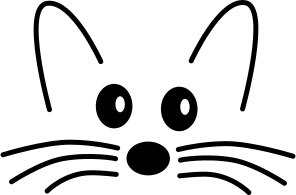
\includegraphics[width=1.4em]{squeak-logo}}}
\iftoshelse{
	\usepackage{marginnote}
		\renewcommand*{\marginfont}{\footnotesize}
	\newcommand{\vartriangleout}{\ifthenelse{\isodd{\thepage}}{\vartriangleright}{\vartriangleleft}}
	\newcommand{\dothisicon}{\fcolorbox{blue!65}{white}{\highlight{$\vartriangleout$}}}
	\newcommand{\dothis}[1]{%
		\noindent\par\noindent
		{\reversemarginpar
			\marginnote{\fcolorbox{blue!65}{white}{\highlight{$\vartriangleout$}}}}
		%\MarginLabel{do this}
		\noindent\emph{#1}
		\nopagebreak}
}{
	\newcommand{\dothisicon}{\raisebox{-.5ex}{
\includegraphics[height=1.2em]{pharo}}}
	\newcommand{\dothis}[1]{%
		\medskip
		\noindent\dothisicon
		\ifx#1\empty\else\quad\emph{#1}\fi
		\par\smallskip\nopagebreak}
}
%===> NEW VERSION <===
% NB: To use this in an individual chapter, you must set:
%\graphicspath{{figures/} {../figures/}}
% at the head of the chapter.  Don't forget the final /
%=============================================================
%:Reader hints (hint)
%
% Indicates a non-obvious consequence
\newcommand{\hint}[1]{\vspace{1ex}\noindent\fbox{\textsc{Hint}} \emph{#1}}
%=================================================================
% graphics for Morphic handles
\newcommand{\grabHandle}{\raisebox{-0.2ex}{
\includegraphics[width=1em]{blackHandle}}}
\newcommand{\moveHandle}{\raisebox{-0.2ex}{
\includegraphics[width=1em]{moveHandle}}}
\newcommand{\debugHandle}{\raisebox{-0.2ex}{
\includegraphics[width=1em]{debugHandle}}}
%=============================================================
%:Highlighting Important stuff (doublebox)
%
% From Seaside book ...
\newsavebox{\SavedText}
\newlength{\InnerBoxRule}\setlength{\InnerBoxRule}{.75\fboxrule}
\newlength{\OuterBoxRule}\setlength{\OuterBoxRule}{1.5\fboxrule}
\newlength{\BoxSeparation}\setlength{\BoxSeparation}{1.5\fboxrule}
\addtolength{\BoxSeparation}{.5pt}
\newlength{\SaveBoxSep}\setlength{\SaveBoxSep}{2\fboxsep}
%
\newenvironment{doublebox}{\begin{lrbox}{\SavedText}
    \begin{minipage}{.75\textwidth}}
    {\end{minipage}\end{lrbox}\begin{center}
    \setlength{\fboxsep}{\BoxSeparation}\setlength{\fboxrule}{\OuterBoxRule}
    \fbox{\setlength{\fboxsep}{\SaveBoxSep}\setlength{\fboxrule}{\InnerBoxRule}%
      \fbox{\usebox{\SavedText}}}
  \end{center}}
% Use this:
\newcommand{\important}[1]{\begin{doublebox}#1\end{doublebox}}
%=============================================================
%:Section depth
\setcounter{secnumdepth}{2}
%% for this to happen start the file with
%\ifx\wholebook\relax\else
%% $Author$
% $Date$
% $Revision$

% HISTORY:
% 2006-10-31 - Oscar code macros
% ...

%=============================================================
% NB: documentclass must be set in main document.
% Allows book to be generated in multiple formats.
%=============================================================
%:Packages
\usepackage[T1]{fontenc}  %%%%%% really important to get the code directly in the text!
\usepackage{lmodern}
%\usepackage[scaled=0.85]{bookmanx} % needs another scale factor if used with \renewcommand{\sfdefault}{cmbr}
\usepackage{palatino}
\usepackage[scaled=0.85]{helvet}
\usepackage[protrusion,expansion=false]{microtype}
\usepackage{graphicx}
\usepackage{theorem}
\usepackage[english]{babel}
% ON: pdfsync breaks the use of p{width} for tabular columns!
\ifdefined\usepdfsync\usepackage{pdfsync}\fi % Requires texlive 2007
%=============================================================
%:More packages
%Stef should check which ones are used!
%\usepackage{picinpar}
%\usepackage{layout}
%\usepackage{color}
%\usepackage{enum}
%\usepackage{a4wide}
% \usepackage{fancyhdr}
\usepackage{ifthen}
\usepackage{float}
\usepackage{longtable}
\usepackage{makeidx}
\usepackage[nottoc]{tocbibind}
\usepackage{multicol}
\usepackage{booktabs}	% book-style tables
\usepackage{topcapt}	% enables \topcaption
\usepackage{multirow}
\usepackage{tabularx}
%\usepackage[bottom]{footmisc}
\usepackage{xspace}
\usepackage{alltt}
\usepackage{amssymb,textcomp}
\usepackage[usenames,dvipsnames]{color}
%\usepackage{colortbl}
\usepackage[hang]{subfigure}\makeatletter\def\p@subfigure{\thefigure\,}\makeatother
\usepackage{rotating}
\usepackage{enumitem}	% apb: allows more control over tags in enumerations
\usepackage{verbatim}     % for comment environment
\usepackage{varioref}	% for page references that work
\labelformat{footnote}{\thechapter--#1} % to distinguish citations from jurabib
\usepackage{needspace}
\usepackage{isodateo} % enable \isodate
\usepackage[newparttoc,pagestyles]{titlesec}
\usepackage{titletoc}
\usepackage{wrapfig}

\usepackage[
	super,
	citefull=first,
	authorformat={allreversed,and},
	titleformat={commasep,italic}
]{jurabib} % citations as footnotes
\usepackage[
	colorlinks=true,
	linkcolor=black,
	urlcolor=black,
	citecolor=black
]{hyperref}   % should come last
%=============================================================
%:PDF version
\pdfminorversion=3 % Set PDF to 1.3 for Lulu
%=============================================================
%:URL style
\makeatletter
\def\url@leostyle{%
  \@ifundefined{selectfont}{\def\UrlFont{\sf}}{\def\UrlFont{\sffamily}}}
\makeatother
% Now actually use the newly defined style.
\urlstyle{leo}
%=============================================================
%:Booleans
\newboolean{lulu}
\setboolean{lulu}{false}
\newcommand{\ifluluelse}[2]{\ifthenelse{\boolean{lulu}}{#1}{#2}}
%=============================================================
%:Names
\newcommand{\SUnit}{SUnit\xspace}
\newcommand{\sunit}{SUnit\xspace}
\newcommand{\xUnit}{$x$Unit\xspace}
\newcommand{\JUnit}{JUnit\xspace}
\newcommand{\st}{Smalltalk\xspace}
\newcommand{\pharo}{Pharo\xspace} % Use this, not \Pharo
%\newcommand{\sqmap}{SqueakMap\xspace}
\newcommand{\squeak}{Squeak\xspace} % use this, not \Squeak or \sq
\newcommand{\sqsrc}{SqueakSource\xspace}
\newcommand{\sbe}{\url{http://SqueakByExample.org}\xspace}
\newcommand{\pharoweb}{\url{http://pharo-project.org}\xspace}
\newcommand{\pbe}{\url{http://PharoByExample.org}\xspace}
\newcommand{\sba}{\url{http://SquareBracketAssociates.org}\xspace}
\newcommand{\bam}{\lct{Bounc\-ing\-Atoms\-Morph}\xspace}
%=============================================================
%:Markup macros for proof-reading
\usepackage[normalem]{ulem} % for \sout
\usepackage{xcolor}
\newcommand{\ra}{$\rightarrow$}
\newcommand{\ugh}[1]{\textcolor{red}{\uwave{#1}}} % please rephrase
\newcommand{\ins}[1]{\textcolor{blue}{\uline{#1}}} % please insert
\newcommand{\del}[1]{\textcolor{red}{\sout{#1}}} % please delete
\newcommand{\chg}[2]{\textcolor{red}{\sout{#1}}{\ra}\textcolor{blue}{\uline{#2}}} % please change
%=============================================================
%:Editorial comment macros
%\newcommand{\nnbb}[2]{
%    % \fbox{\bfseries\sffamily\scriptsize#1}
%    \fcolorbox{gray}{yellow}{\bfseries\sffamily\scriptsize#1}
%    {\sf\small$\blacktriangleright$\textit{#2}$\blacktriangleleft$}
%   }
\newcommand{\yellowbox}[1]{\fcolorbox{gray}{yellow}{\bfseries\sffamily\scriptsize#1}}
\newcommand{\triangles}[1]{{\sf\small$\blacktriangleright$\textit{#1}$\blacktriangleleft$}}
\newcommand{\nnbb}[2]{\yellowbox{#1} \triangles{#2}}
\newcommand{\fix}{\yellowbox{FIX!}}
\newcommand{\here}{\yellowbox{CONTINUE HERE!}}
% editor macros
\newcommand{\apl}[1]{\nnbb{Alain}{#1}} % Alain
\newcommand{\ab}[1]{\nnbb{Andrew}{#1}} % Black
\newcommand{\sd}[1]{\nnbb{St\'{e}f}{#1}} % Ducasse
\newcommand{\gl}[1]{\nnbb{Guillaume}{#1}} % Ducasse
\newcommand{\cd}[1]{\nnbb{Christophe}{#1}} % Ducasse
\newcommand{\sig}[1]{\nnbb{Igor}{#1}} % Igor
\newcommand{\dc}[1]{\nnbb{DamienC}{#1}} % Ducasse
\newcommand{\md}[1]{\nnbb{Marcus}{#1}} % Denker
\newcommand{\on}[1]{\nnbb{Oscar}{#1}} % Nierstrasz
\newcommand{\damien}[1]{\nnbb{Damien}{#1}} % Pollet
\newcommand{\lr}[1]{\nnbb{Lukas}{#1}} % Renggli
\newcommand{\orla}[1]{\nnbb{Orla}{#1}} % Greevy
\newcommand{\alex}[1]{\nnbb{Alex}{#1}} % Bergel
\newcommand{\alx}[1]{\nnbb{Alex}{#1}} % Bergel
\newcommand{\dr}[1]{\nnbb{David}{#1}} % Roethlisberger
\newcommand{\ja}[1]{\nnbb{Jannik}{#1}} % Laval
\newcommand{\cb}[1]{\nnbb{Camillo}{#1}} % Bruni
\newcommand{\jr}[1]{\nnbb{Jorge}{#1}} % Ressia
\newcommand{\jb}[1]{\nnbb{JB}{#1}} % JB
\newcommand{\jp}[1]{\nnbb{Javier}{#1}} % Pimas
\newcommand{\fp}[1]{\nnbb{Fabrizio}{#1}} % Perin
\newcommand{\michael}[1]{\nnbb{Michael}{#1}} % Davies
\newcommand{\ew}[1]{\nnbb{Erwann}{#1}} % Wernli
\newcommand{\mb}[1]{\nnbb{Martial}{#1}} % Boniou
\newcommand{\hw}[1]{\nnbb{Hernan}{#1}} % Wilkinson
\newcommand{\ben}[1]{\nnbb{Benjamin}{#1}} % Benjamin Van Ryseghem
\newcommand{\hjo}[1]{\nnbb{HwaJong}{#1}} % HwaJong Oh aka daliot
\newcommand{\ml}[1]{\nnbb{Max}{#1}} % Max Leske
\newcommand{\mmp}[1]{\nnbb{Mariano}{#1}} % Mariano Martinez Peck
\newcommand{\luc}[1]{\nnbb{Luc}{#1}} % Luc Fabresse
\newcommand{\dkl}[1]{\nnbb{Daniel}{#1}} % Daniel Lyons
\newcommand{\vu}[1]{\nnbb{Veronica}{#1}} % Veronica Uquillas Gomez
\newcommand{\martin}[1]{\nnbb{Martin}{#1}} % Martin Dias
\newcommand{\vp}[1]{\nnbb{Vanessa}{#1}} % Vanessa Pena
\newcommand{\gp}[1]{\nnbb{Guille}{#1}} % Guillermo Polito

%=============================================================
%:Abbreviation macros
\newcommand{\ie}{\emph{i.e.},\xspace}
\newcommand{\eg}{\emph{e.g.},\xspace}
\newcommand{\etc}{etc.\xspace}
%=============================================================
%:Cross reference macros
\newcommand{\charef}[1]{Chapter~\ref{cha:#1}\xspace}
\newcommand{\secref}[1]{Section~\ref{sec:#1}\xspace}
\newcommand{\figref}[1]{Figure~\ref{fig:#1}\xspace}
\newcommand{\Figref}[1]{Figure~\ref{fig:#1}\xspace}
\newcommand{\appref}[1]{Appendix~\ref{app:#1}\xspace}
\newcommand{\tabref}[1]{Table~\ref{tab:#1}\xspace}
\newcommand{\faqref}[1]{FAQ~\ref{faq:#1}, p.~\pageref{faq:#1}\xspace}
% APB: I removed trailing \xspace commands from these macros because
% \xspace mostly doesn't work.  If you want a space after your
% references, type one!
% ON: xspace has always worked just fine for me!  Please leave them in.
%
\newcommand{\ruleref}[1]{\ref{rule:#1}\xspace}
%
\newcommand{\egref}[1]{example~\ref{eg:#1}\xspace}
\newcommand{\Egref}[1]{Example~\ref{eg:#1}\xspace}
%
\newcommand{\scrref}[1]{script~\ref{scr:#1}\xspace}
\newcommand{\Scrref}[1]{Script~\ref{scr:#1}\xspace}
\newcommand{\tscrref}[1]{the script~\ref{scr:#1}\xspace}
\newcommand{\Tscrref}[1]{The script~\ref{scr:#1}\xspace}
%
\newcommand{\mthref}[1]{method~\ref{mth:#1}\xspace}
\newcommand{\mthsref}[1]{methods~\ref{mth:#1}\xspace}
\newcommand{\Mthref}[1]{Method~\ref{mth:#1}\xspace}
\newcommand{\tmthref}[1]{the method~\ref{mth:#1}\xspace}
\newcommand{\Tmthref}[1]{The method~\ref{mth:#1}\xspace}
%
\newcommand{\clsref}[1]{class~\ref{cls:#1}\xspace}
\newcommand{\tclsref}[1]{the class~\ref{cls:#1}\xspace}
\newcommand{\Tclsref}[1]{The class~\ref{cls:#1}\xspace}

\newcommand{\chalabel}[1]{\label{cha:#1}}
\newcommand{\seclabel}[1]{\label{sec:#1}}
\newcommand{\figlabel}[1]{\label{fig:#1}}
\newcommand{\tablabel}[1]{\label{tab:#1}}
\newcommand{\rulelabel}[1]{\label{rule:#1}}
\newcommand{\eglabel}[1]{\label{eg:#1}}
\newcommand{\scrlabel}[1]{\label{scr:#1}}
\newcommand{\mthlabel}[1]{\label{mth:#1}}
\newcommand{\clslabel}[1]{\label{cls:#1}}
\newcommand{\faqlabel}[1]{\label{faq:#1}}
%=============================================================
%:Menu item macro
% for menu items, so we can change our minds on how to print them! (apb)
\definecolor{lightgray}{gray}{0.89}
\newcommand{\menu}[1]{{%
	\setlength{\fboxsep}{0pt}%
	\colorbox{lightgray}{{{\upshape\sffamily\strut \,#1\,}}}}}
\newcommand{\link}[1]{{%
	\fontfamily{lmr}\selectfont
 	\upshape{\sffamily \underline{#1}}}}
% For submenu items:
\newcommand{\go}{\,$\triangleright$\,}
% \newcommand{\go}{\,$\blacktriangleright$\,}
% For keyboard shortcuts:
%\newcommand{\short}[1]{\mbox{$\langle${\sc CMD}$\rangle$-#1}\xspace}
\newcommand{\short}[1]{\mbox{{\sc cmd}\hspace{0.08em}--\hspace{0.09em}#1}\xspace}
% For buttons:
\newcommand{\button}[1]{{%
	\setlength{\fboxsep}{0pt}%
	\fbox{{\upshape\sffamily\strut \,#1\,}}}}
% NB: The button macro does not work within captions -- incompatible with xcolor package :-(
\newcommand{\toolsflap}{\textit{Tools} flap\xspace}
%=============================================================
%:Mouse clicks
\newcommand{\click}{click\xspace} % RED
\newcommand{\actclick}{action-click\xspace} % YELLOW
\newcommand{\metaclick}{meta-click\xspace} % BLUE
\newcommand{\Click}{Click\xspace} % RED
\newcommand{\Actclick}{Action-click\xspace} % YELLOW
\newcommand{\Metaclick}{Meta-click\xspace} % BLUE
%=============================================================
%:ToSh macros
\newboolean{tosh}
\setboolean{tosh}{false}
\newcommand{\iftoshelse}[2]{\ifthenelse{\boolean{tosh}}{#1}{#2}}
%=============================================================
%:ToSh colors
%\newcommand{\highlightcolor}{\color{blue!65}}
%\newcommand{\boxcolor}{\color{gray!25}}
\newcommand{\highlight}[1]{\textcolor{blue!65}{#1}}
%\newcommand{\codecolor}{\color{blue!65}}
%%\setlength{\fboxrule}{2pt}
%\newcommand{\asPict}[1]{%
%	{\Large\highlight{#1}}}
%=============================================================
%:Reader cues (do this)
%
% Indicate something the reader should try out.
% \newcommand{\dothisicon}{\raisebox{-.5ex}{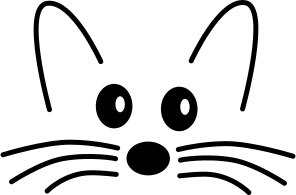
\includegraphics[width=1.4em]{squeak-logo}}}
\iftoshelse{
	\usepackage{marginnote}
		\renewcommand*{\marginfont}{\footnotesize}
	\newcommand{\vartriangleout}{\ifthenelse{\isodd{\thepage}}{\vartriangleright}{\vartriangleleft}}
	\newcommand{\dothisicon}{\fcolorbox{blue!65}{white}{\highlight{$\vartriangleout$}}}
	\newcommand{\dothis}[1]{%
		\noindent\par\noindent
		{\reversemarginpar
			\marginnote{\fcolorbox{blue!65}{white}{\highlight{$\vartriangleout$}}}}
		%\MarginLabel{do this}
		\noindent\emph{#1}
		\nopagebreak}
}{
	\newcommand{\dothisicon}{\raisebox{-.5ex}{
\includegraphics[height=1.2em]{pharo}}}
	\newcommand{\dothis}[1]{%
		\medskip
		\noindent\dothisicon
		\ifx#1\empty\else\quad\emph{#1}\fi
		\par\smallskip\nopagebreak}
}
%===> NEW VERSION <===
% NB: To use this in an individual chapter, you must set:
%\graphicspath{{figures/} {../figures/}}
% at the head of the chapter.  Don't forget the final /
%=============================================================
%:Reader hints (hint)
%
% Indicates a non-obvious consequence
\newcommand{\hint}[1]{\vspace{1ex}\noindent\fbox{\textsc{Hint}} \emph{#1}}
%=================================================================
% graphics for Morphic handles
\newcommand{\grabHandle}{\raisebox{-0.2ex}{
\includegraphics[width=1em]{blackHandle}}}
\newcommand{\moveHandle}{\raisebox{-0.2ex}{
\includegraphics[width=1em]{moveHandle}}}
\newcommand{\debugHandle}{\raisebox{-0.2ex}{
\includegraphics[width=1em]{debugHandle}}}
%=============================================================
%:Highlighting Important stuff (doublebox)
%
% From Seaside book ...
\newsavebox{\SavedText}
\newlength{\InnerBoxRule}\setlength{\InnerBoxRule}{.75\fboxrule}
\newlength{\OuterBoxRule}\setlength{\OuterBoxRule}{1.5\fboxrule}
\newlength{\BoxSeparation}\setlength{\BoxSeparation}{1.5\fboxrule}
\addtolength{\BoxSeparation}{.5pt}
\newlength{\SaveBoxSep}\setlength{\SaveBoxSep}{2\fboxsep}
%
\newenvironment{doublebox}{\begin{lrbox}{\SavedText}
    \begin{minipage}{.75\textwidth}}
    {\end{minipage}\end{lrbox}\begin{center}
    \setlength{\fboxsep}{\BoxSeparation}\setlength{\fboxrule}{\OuterBoxRule}
    \fbox{\setlength{\fboxsep}{\SaveBoxSep}\setlength{\fboxrule}{\InnerBoxRule}%
      \fbox{\usebox{\SavedText}}}
  \end{center}}
% Use this:
\newcommand{\important}[1]{\begin{doublebox}#1\end{doublebox}}
%=============================================================
%:Section depth
\setcounter{secnumdepth}{2}
%% for this to happen start the file with
%\ifx\wholebook\relax\else
%% $Author$
% $Date$
% $Revision$

% HISTORY:
% 2006-10-31 - Oscar code macros
% ...

%=============================================================
% NB: documentclass must be set in main document.
% Allows book to be generated in multiple formats.
%=============================================================
%:Packages
\usepackage[T1]{fontenc}  %%%%%% really important to get the code directly in the text!
\usepackage{lmodern}
%\usepackage[scaled=0.85]{bookmanx} % needs another scale factor if used with \renewcommand{\sfdefault}{cmbr}
\usepackage{palatino}
\usepackage[scaled=0.85]{helvet}
\usepackage[protrusion,expansion=false]{microtype}
\usepackage{graphicx}
\usepackage{theorem}
\usepackage[english]{babel}
% ON: pdfsync breaks the use of p{width} for tabular columns!
\ifdefined\usepdfsync\usepackage{pdfsync}\fi % Requires texlive 2007
%=============================================================
%:More packages
%Stef should check which ones are used!
%\usepackage{picinpar}
%\usepackage{layout}
%\usepackage{color}
%\usepackage{enum}
%\usepackage{a4wide}
% \usepackage{fancyhdr}
\usepackage{ifthen}
\usepackage{float}
\usepackage{longtable}
\usepackage{makeidx}
\usepackage[nottoc]{tocbibind}
\usepackage{multicol}
\usepackage{booktabs}	% book-style tables
\usepackage{topcapt}	% enables \topcaption
\usepackage{multirow}
\usepackage{tabularx}
%\usepackage[bottom]{footmisc}
\usepackage{xspace}
\usepackage{alltt}
\usepackage{amssymb,textcomp}
\usepackage[usenames,dvipsnames]{color}
%\usepackage{colortbl}
\usepackage[hang]{subfigure}\makeatletter\def\p@subfigure{\thefigure\,}\makeatother
\usepackage{rotating}
\usepackage{enumitem}	% apb: allows more control over tags in enumerations
\usepackage{verbatim}     % for comment environment
\usepackage{varioref}	% for page references that work
\labelformat{footnote}{\thechapter--#1} % to distinguish citations from jurabib
\usepackage{needspace}
\usepackage{isodateo} % enable \isodate
\usepackage[newparttoc,pagestyles]{titlesec}
\usepackage{titletoc}
\usepackage{wrapfig}

\usepackage[
	super,
	citefull=first,
	authorformat={allreversed,and},
	titleformat={commasep,italic}
]{jurabib} % citations as footnotes
\usepackage[
	colorlinks=true,
	linkcolor=black,
	urlcolor=black,
	citecolor=black
]{hyperref}   % should come last
%=============================================================
%:PDF version
\pdfminorversion=3 % Set PDF to 1.3 for Lulu
%=============================================================
%:URL style
\makeatletter
\def\url@leostyle{%
  \@ifundefined{selectfont}{\def\UrlFont{\sf}}{\def\UrlFont{\sffamily}}}
\makeatother
% Now actually use the newly defined style.
\urlstyle{leo}
%=============================================================
%:Booleans
\newboolean{lulu}
\setboolean{lulu}{false}
\newcommand{\ifluluelse}[2]{\ifthenelse{\boolean{lulu}}{#1}{#2}}
%=============================================================
%:Names
\newcommand{\SUnit}{SUnit\xspace}
\newcommand{\sunit}{SUnit\xspace}
\newcommand{\xUnit}{$x$Unit\xspace}
\newcommand{\JUnit}{JUnit\xspace}
\newcommand{\st}{Smalltalk\xspace}
\newcommand{\pharo}{Pharo\xspace} % Use this, not \Pharo
%\newcommand{\sqmap}{SqueakMap\xspace}
\newcommand{\squeak}{Squeak\xspace} % use this, not \Squeak or \sq
\newcommand{\sqsrc}{SqueakSource\xspace}
\newcommand{\sbe}{\url{http://SqueakByExample.org}\xspace}
\newcommand{\pharoweb}{\url{http://pharo-project.org}\xspace}
\newcommand{\pbe}{\url{http://PharoByExample.org}\xspace}
\newcommand{\sba}{\url{http://SquareBracketAssociates.org}\xspace}
\newcommand{\bam}{\lct{Bounc\-ing\-Atoms\-Morph}\xspace}
%=============================================================
%:Markup macros for proof-reading
\usepackage[normalem]{ulem} % for \sout
\usepackage{xcolor}
\newcommand{\ra}{$\rightarrow$}
\newcommand{\ugh}[1]{\textcolor{red}{\uwave{#1}}} % please rephrase
\newcommand{\ins}[1]{\textcolor{blue}{\uline{#1}}} % please insert
\newcommand{\del}[1]{\textcolor{red}{\sout{#1}}} % please delete
\newcommand{\chg}[2]{\textcolor{red}{\sout{#1}}{\ra}\textcolor{blue}{\uline{#2}}} % please change
%=============================================================
%:Editorial comment macros
%\newcommand{\nnbb}[2]{
%    % \fbox{\bfseries\sffamily\scriptsize#1}
%    \fcolorbox{gray}{yellow}{\bfseries\sffamily\scriptsize#1}
%    {\sf\small$\blacktriangleright$\textit{#2}$\blacktriangleleft$}
%   }
\newcommand{\yellowbox}[1]{\fcolorbox{gray}{yellow}{\bfseries\sffamily\scriptsize#1}}
\newcommand{\triangles}[1]{{\sf\small$\blacktriangleright$\textit{#1}$\blacktriangleleft$}}
\newcommand{\nnbb}[2]{\yellowbox{#1} \triangles{#2}}
\newcommand{\fix}{\yellowbox{FIX!}}
\newcommand{\here}{\yellowbox{CONTINUE HERE!}}
% editor macros
\newcommand{\apl}[1]{\nnbb{Alain}{#1}} % Alain
\newcommand{\ab}[1]{\nnbb{Andrew}{#1}} % Black
\newcommand{\sd}[1]{\nnbb{St\'{e}f}{#1}} % Ducasse
\newcommand{\gl}[1]{\nnbb{Guillaume}{#1}} % Ducasse
\newcommand{\cd}[1]{\nnbb{Christophe}{#1}} % Ducasse
\newcommand{\sig}[1]{\nnbb{Igor}{#1}} % Igor
\newcommand{\dc}[1]{\nnbb{DamienC}{#1}} % Ducasse
\newcommand{\md}[1]{\nnbb{Marcus}{#1}} % Denker
\newcommand{\on}[1]{\nnbb{Oscar}{#1}} % Nierstrasz
\newcommand{\damien}[1]{\nnbb{Damien}{#1}} % Pollet
\newcommand{\lr}[1]{\nnbb{Lukas}{#1}} % Renggli
\newcommand{\orla}[1]{\nnbb{Orla}{#1}} % Greevy
\newcommand{\alex}[1]{\nnbb{Alex}{#1}} % Bergel
\newcommand{\alx}[1]{\nnbb{Alex}{#1}} % Bergel
\newcommand{\dr}[1]{\nnbb{David}{#1}} % Roethlisberger
\newcommand{\ja}[1]{\nnbb{Jannik}{#1}} % Laval
\newcommand{\cb}[1]{\nnbb{Camillo}{#1}} % Bruni
\newcommand{\jr}[1]{\nnbb{Jorge}{#1}} % Ressia
\newcommand{\jb}[1]{\nnbb{JB}{#1}} % JB
\newcommand{\jp}[1]{\nnbb{Javier}{#1}} % Pimas
\newcommand{\fp}[1]{\nnbb{Fabrizio}{#1}} % Perin
\newcommand{\michael}[1]{\nnbb{Michael}{#1}} % Davies
\newcommand{\ew}[1]{\nnbb{Erwann}{#1}} % Wernli
\newcommand{\mb}[1]{\nnbb{Martial}{#1}} % Boniou
\newcommand{\hw}[1]{\nnbb{Hernan}{#1}} % Wilkinson
\newcommand{\ben}[1]{\nnbb{Benjamin}{#1}} % Benjamin Van Ryseghem
\newcommand{\hjo}[1]{\nnbb{HwaJong}{#1}} % HwaJong Oh aka daliot
\newcommand{\ml}[1]{\nnbb{Max}{#1}} % Max Leske
\newcommand{\mmp}[1]{\nnbb{Mariano}{#1}} % Mariano Martinez Peck
\newcommand{\luc}[1]{\nnbb{Luc}{#1}} % Luc Fabresse
\newcommand{\dkl}[1]{\nnbb{Daniel}{#1}} % Daniel Lyons
\newcommand{\vu}[1]{\nnbb{Veronica}{#1}} % Veronica Uquillas Gomez
\newcommand{\martin}[1]{\nnbb{Martin}{#1}} % Martin Dias
\newcommand{\vp}[1]{\nnbb{Vanessa}{#1}} % Vanessa Pena
\newcommand{\gp}[1]{\nnbb{Guille}{#1}} % Guillermo Polito

%=============================================================
%:Abbreviation macros
\newcommand{\ie}{\emph{i.e.},\xspace}
\newcommand{\eg}{\emph{e.g.},\xspace}
\newcommand{\etc}{etc.\xspace}
%=============================================================
%:Cross reference macros
\newcommand{\charef}[1]{Chapter~\ref{cha:#1}\xspace}
\newcommand{\secref}[1]{Section~\ref{sec:#1}\xspace}
\newcommand{\figref}[1]{Figure~\ref{fig:#1}\xspace}
\newcommand{\Figref}[1]{Figure~\ref{fig:#1}\xspace}
\newcommand{\appref}[1]{Appendix~\ref{app:#1}\xspace}
\newcommand{\tabref}[1]{Table~\ref{tab:#1}\xspace}
\newcommand{\faqref}[1]{FAQ~\ref{faq:#1}, p.~\pageref{faq:#1}\xspace}
% APB: I removed trailing \xspace commands from these macros because
% \xspace mostly doesn't work.  If you want a space after your
% references, type one!
% ON: xspace has always worked just fine for me!  Please leave them in.
%
\newcommand{\ruleref}[1]{\ref{rule:#1}\xspace}
%
\newcommand{\egref}[1]{example~\ref{eg:#1}\xspace}
\newcommand{\Egref}[1]{Example~\ref{eg:#1}\xspace}
%
\newcommand{\scrref}[1]{script~\ref{scr:#1}\xspace}
\newcommand{\Scrref}[1]{Script~\ref{scr:#1}\xspace}
\newcommand{\tscrref}[1]{the script~\ref{scr:#1}\xspace}
\newcommand{\Tscrref}[1]{The script~\ref{scr:#1}\xspace}
%
\newcommand{\mthref}[1]{method~\ref{mth:#1}\xspace}
\newcommand{\mthsref}[1]{methods~\ref{mth:#1}\xspace}
\newcommand{\Mthref}[1]{Method~\ref{mth:#1}\xspace}
\newcommand{\tmthref}[1]{the method~\ref{mth:#1}\xspace}
\newcommand{\Tmthref}[1]{The method~\ref{mth:#1}\xspace}
%
\newcommand{\clsref}[1]{class~\ref{cls:#1}\xspace}
\newcommand{\tclsref}[1]{the class~\ref{cls:#1}\xspace}
\newcommand{\Tclsref}[1]{The class~\ref{cls:#1}\xspace}

\newcommand{\chalabel}[1]{\label{cha:#1}}
\newcommand{\seclabel}[1]{\label{sec:#1}}
\newcommand{\figlabel}[1]{\label{fig:#1}}
\newcommand{\tablabel}[1]{\label{tab:#1}}
\newcommand{\rulelabel}[1]{\label{rule:#1}}
\newcommand{\eglabel}[1]{\label{eg:#1}}
\newcommand{\scrlabel}[1]{\label{scr:#1}}
\newcommand{\mthlabel}[1]{\label{mth:#1}}
\newcommand{\clslabel}[1]{\label{cls:#1}}
\newcommand{\faqlabel}[1]{\label{faq:#1}}
%=============================================================
%:Menu item macro
% for menu items, so we can change our minds on how to print them! (apb)
\definecolor{lightgray}{gray}{0.89}
\newcommand{\menu}[1]{{%
	\setlength{\fboxsep}{0pt}%
	\colorbox{lightgray}{{{\upshape\sffamily\strut \,#1\,}}}}}
\newcommand{\link}[1]{{%
	\fontfamily{lmr}\selectfont
 	\upshape{\sffamily \underline{#1}}}}
% For submenu items:
\newcommand{\go}{\,$\triangleright$\,}
% \newcommand{\go}{\,$\blacktriangleright$\,}
% For keyboard shortcuts:
%\newcommand{\short}[1]{\mbox{$\langle${\sc CMD}$\rangle$-#1}\xspace}
\newcommand{\short}[1]{\mbox{{\sc cmd}\hspace{0.08em}--\hspace{0.09em}#1}\xspace}
% For buttons:
\newcommand{\button}[1]{{%
	\setlength{\fboxsep}{0pt}%
	\fbox{{\upshape\sffamily\strut \,#1\,}}}}
% NB: The button macro does not work within captions -- incompatible with xcolor package :-(
\newcommand{\toolsflap}{\textit{Tools} flap\xspace}
%=============================================================
%:Mouse clicks
\newcommand{\click}{click\xspace} % RED
\newcommand{\actclick}{action-click\xspace} % YELLOW
\newcommand{\metaclick}{meta-click\xspace} % BLUE
\newcommand{\Click}{Click\xspace} % RED
\newcommand{\Actclick}{Action-click\xspace} % YELLOW
\newcommand{\Metaclick}{Meta-click\xspace} % BLUE
%=============================================================
%:ToSh macros
\newboolean{tosh}
\setboolean{tosh}{false}
\newcommand{\iftoshelse}[2]{\ifthenelse{\boolean{tosh}}{#1}{#2}}
%=============================================================
%:ToSh colors
%\newcommand{\highlightcolor}{\color{blue!65}}
%\newcommand{\boxcolor}{\color{gray!25}}
\newcommand{\highlight}[1]{\textcolor{blue!65}{#1}}
%\newcommand{\codecolor}{\color{blue!65}}
%%\setlength{\fboxrule}{2pt}
%\newcommand{\asPict}[1]{%
%	{\Large\highlight{#1}}}
%=============================================================
%:Reader cues (do this)
%
% Indicate something the reader should try out.
% \newcommand{\dothisicon}{\raisebox{-.5ex}{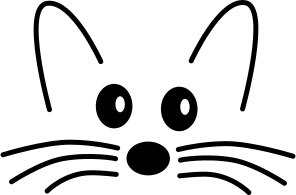
\includegraphics[width=1.4em]{squeak-logo}}}
\iftoshelse{
	\usepackage{marginnote}
		\renewcommand*{\marginfont}{\footnotesize}
	\newcommand{\vartriangleout}{\ifthenelse{\isodd{\thepage}}{\vartriangleright}{\vartriangleleft}}
	\newcommand{\dothisicon}{\fcolorbox{blue!65}{white}{\highlight{$\vartriangleout$}}}
	\newcommand{\dothis}[1]{%
		\noindent\par\noindent
		{\reversemarginpar
			\marginnote{\fcolorbox{blue!65}{white}{\highlight{$\vartriangleout$}}}}
		%\MarginLabel{do this}
		\noindent\emph{#1}
		\nopagebreak}
}{
	\newcommand{\dothisicon}{\raisebox{-.5ex}{
\includegraphics[height=1.2em]{pharo}}}
	\newcommand{\dothis}[1]{%
		\medskip
		\noindent\dothisicon
		\ifx#1\empty\else\quad\emph{#1}\fi
		\par\smallskip\nopagebreak}
}
%===> NEW VERSION <===
% NB: To use this in an individual chapter, you must set:
%\graphicspath{{figures/} {../figures/}}
% at the head of the chapter.  Don't forget the final /
%=============================================================
%:Reader hints (hint)
%
% Indicates a non-obvious consequence
\newcommand{\hint}[1]{\vspace{1ex}\noindent\fbox{\textsc{Hint}} \emph{#1}}
%=================================================================
% graphics for Morphic handles
\newcommand{\grabHandle}{\raisebox{-0.2ex}{
\includegraphics[width=1em]{blackHandle}}}
\newcommand{\moveHandle}{\raisebox{-0.2ex}{
\includegraphics[width=1em]{moveHandle}}}
\newcommand{\debugHandle}{\raisebox{-0.2ex}{
\includegraphics[width=1em]{debugHandle}}}
%=============================================================
%:Highlighting Important stuff (doublebox)
%
% From Seaside book ...
\newsavebox{\SavedText}
\newlength{\InnerBoxRule}\setlength{\InnerBoxRule}{.75\fboxrule}
\newlength{\OuterBoxRule}\setlength{\OuterBoxRule}{1.5\fboxrule}
\newlength{\BoxSeparation}\setlength{\BoxSeparation}{1.5\fboxrule}
\addtolength{\BoxSeparation}{.5pt}
\newlength{\SaveBoxSep}\setlength{\SaveBoxSep}{2\fboxsep}
%
\newenvironment{doublebox}{\begin{lrbox}{\SavedText}
    \begin{minipage}{.75\textwidth}}
    {\end{minipage}\end{lrbox}\begin{center}
    \setlength{\fboxsep}{\BoxSeparation}\setlength{\fboxrule}{\OuterBoxRule}
    \fbox{\setlength{\fboxsep}{\SaveBoxSep}\setlength{\fboxrule}{\InnerBoxRule}%
      \fbox{\usebox{\SavedText}}}
  \end{center}}
% Use this:
\newcommand{\important}[1]{\begin{doublebox}#1\end{doublebox}}
%=============================================================
%:Section depth
\setcounter{secnumdepth}{2}
%% for this to happen start the file with
%\ifx\wholebook\relax\else
%\input{../common.tex}
%\begin{document}
%\fi
% and terminate by
% \ifx\wholebook\relax\else\end{document}\fi

\DeclareGraphicsExtensions{.pdf, .jpg, .png}
%=============================================================
%:PDF setup
\hypersetup{
%   a4paper,
%   pdfstartview=FitV,
%   colorlinks,
%   linkcolor=darkblue,
%   citecolor=darkblue,
   pdftitle={Pharo by Example},
   pdfauthor={Andrew P. Black, St\'ephane Ducasse,	Oscar Nierstrasz,
Damien Pollet},
   pdfkeywords={Smalltalk, Squeak, Object-Oriented Programming, OOP},
   pdfsubject={Computer Science}
}
%=============================================================
%:Page layout and appearance
%
% \renewcommand{\headrulewidth}{0pt}
\renewcommand{\chaptermark}[1]{\markboth{#1}{}}
\renewcommand{\sectionmark}[1]{\markright{\thesection\ #1}}
\renewpagestyle{plain}[\small\itshape]{%
	\setheadrule{0pt}%
	\sethead[][][]{}{}{}%
	\setfoot[][][]{}{}{}}
\renewpagestyle{headings}[\small\itshape]{%
	\setheadrule{0pt}%
	\setmarks{chapter}{section}%
	\sethead[\thepage][][\chaptertitle]{\sectiontitle}{}{\thepage}%
	\setfoot[][][]{}{}{}}
%=============================================================
%:Title section setup and TOC numbering depth
\setcounter{secnumdepth}{1}
\setcounter{tocdepth}{1}
\titleformat{\part}[display]{\centering}{\huge\partname\ \thepart}{1em}{\Huge\textbf}[]
\titleformat{\chapter}[display]{}{\huge\chaptertitlename\ \thechapter}{1em}{\Huge\raggedright\textbf}[]
\titlecontents{part}[3pc]{%
		\pagebreak[2]\addvspace{1em plus.4em minus.2em}%
		\leavevmode\large\bfseries}
	{\contentslabel{3pc}}{\hspace*{-3pc}}
	{}[\nopagebreak]
\titlecontents{chapter}[3pc]{%
		\pagebreak[0]\addvspace{1em plus.2em minus.2em}%
		\leavevmode\bfseries}
	{\contentslabel{3pc}}{}
	{\hfill\contentspage}[\nopagebreak]
\dottedcontents{section}[3pc]{}{3pc}{1pc}
\dottedcontents{subsection}[3pc]{}{0pc}{1pc}
% \dottedcontents{subsection}[4.5em]{}{0pt}{1pc}
% Make \cleardoublepage insert really blank pages http://www.tex.ac.uk/cgi-bin/texfaq2html?label=reallyblank
\let\origdoublepage\cleardoublepage
\newcommand{\clearemptydoublepage}{%
  \clearpage
  {\pagestyle{empty}\origdoublepage}}
\let\cleardoublepage\clearemptydoublepage % see http://www.tex.ac.uk/cgi-bin/texfaq2html?label=patch
%=============================================================
%:FAQ macros (for FAQ chapter)
\newtheorem{faq}{FAQ}
\newcommand{\answer}{\paragraph{Answer}\ }
%=============================================================
%:Listings package configuration
% \newcommand{\caret}{\makebox{\raisebox{0.4ex}{\footnotesize{$\wedge$}}}}
\newcommand{\caret}{\^\,}
\newcommand{\escape}{{\sf \textbackslash}}
\definecolor{source}{gray}{0.95}
\usepackage{listings}
\lstdefinelanguage{Smalltalk}{
%  morekeywords={self,super,true,false,nil,thisContext}, % This is overkill
  morestring=[d]',
  morecomment=[s]{"}{"},
  alsoletter={\#:},
  escapechar={!},
  literate=
    {BANG}{!}1
    {CARET}{\^}1
    {UNDERSCORE}{\_}1
    {\\st}{Smalltalk}9 % convenience -- in case \st occurs in code
    % {'}{{\textquotesingle}}1 % replaced by upquote=true in \lstset
    %{_}{{$\leftarrow$}}1
    {>>>}{{\sep}}1
    %{^}{{$\uparrow$}}1
    {~}{{$\sim$}}1
    {-}{{\texttt{-}}}1 %{\textminus}}1 %{-}{\hspace{-0.13em}}{-}}1  % the goal is to make - the same width as +
    % {+}{\sf+}1 %{\raisebox{0.08ex}{+}}}1      % and to raise + off the baseline to match -
    {-->}{{\quad$\longrightarrow$\quad}}3
    {~->}{{\quad$\leadsto$\quad}}3
	, % Don't forget the comma at the end!
  tabsize=4
}[keywords,comments,strings]

\lstset{language=Smalltalk,
	basicstyle=\sffamily,
	keywordstyle=\color{black}\bfseries,
	% stringstyle=\ttfamily, % Ugly! do we really want this? -- on
	mathescape=true,
	showstringspaces=false,
	keepspaces=true,
	breaklines=true,
	breakautoindent=true,
	backgroundcolor=\color{source},
	lineskip={-1pt}, % Ugly hack
	upquote=true, % straight quote; requires textcomp package
	columns=fullflexible} % no fixed width fonts
% In-line code (literal)
% Normally use this for all in-line code:

\newcommand{\ct}{\lstinline[mathescape=false,backgroundcolor=\color{white},basicstyle={\sffamily\upshape}]}
\newcommand{\cts}[1]{{\sffamily{\upshape{#1}}\xspace}}
% apb 2007.8.28 added the \upshape declaration to avoid getting italicized code in \dothis{ } sections.
% In-line code (latex enabled)
% Use this only in special situations where \ct does not work
% (within section headings ...):
\newcommand{\lct}[1]{{\textsf{\textup{#1}}}}
% Use these for system categories and protocols:
\newcommand{\scat}[1]{\emph{\textsf{#1}}\xspace}
\newcommand{\pkg}[1]{\emph{\textsf{#1}}\xspace}
\newcommand{\prot}[1]{\emph{\textsf{#1}}\xspace}
% Code environments
% NB: the arg is for tests
% Only code and example environments may be tests
\lstnewenvironment{code}[1]{%
	\lstset{%
		% frame=lines,
		frame=single,
		framerule=0pt,
		mathescape=false
	}
}{}
\def\ignoredollar#1{}
%=============================================================
%:Code environments (method, script ...)
% NB: the third arg is for tests
% Only code and example environments may be tests
\lstnewenvironment{example}[3][defaultlabel]{%
	\renewcommand{\lstlistingname}{Example}%
	\lstset{
		% frame=lines,
		frame=single,
		framerule=0pt,
		mathescape=false,
		caption={\emph{#2}},
		label={eg:#1}
	}
}{}
\lstnewenvironment{script}[2][defaultlabel]{%
\renewcommand{\lstlistingname}{Script}%
	\lstset{
		% frame=lines,
		frame=single,
		framerule=0pt,
		mathescape=false,
		name={Script},
		caption={\emph{#2}},
		label={scr:#1}
	}
}{}
\lstnewenvironment{method}[2][defaultlabel]{%
	\renewcommand{\lstlistingname}{Method}%
	\lstset{
		% frame=lines,
		frame=single,
		framerule=0pt,
		mathescape=false,
		name={Method},
		caption={\emph{#2}},
		label={mth:#1}
	}
}{}
\lstnewenvironment{methods}[2][defaultlabel]{% just for multiple methods at once
	\renewcommand{\lstlistingname}{Methods}%
	\lstset{
		% frame=lines,
		frame=single,
		framerule=0pt,
		mathescape=false,
		name={Method},
		caption={\emph{#2}},
		label={mth:#1}
	}
}{}
\lstnewenvironment{numMethod}[2][defaultlabel]{%
	\renewcommand{\lstlistingname}{Method}%
	\lstset{
		numbers=left,
		numberstyle={\tiny\sffamily},
		% frame=lines,
		frame=single,
		framerule=0pt,
		mathescape=false,
		name={Method},
		caption={\emph{#2}},
		label={mth:#1}
	}
}{}
\lstnewenvironment{classdef}[2][defaultlabel]{%
	\renewcommand{\lstlistingname}{Class}%
	\lstset{
		% frame=lines,
		frame=single,
		framerule=0pt,
		mathescape=false,
		name={Class},
		caption={\emph{#2}},
		label={cls:#1}
	}
}{}
%=============================================================
%:Reserving space
% Usually need one more line than the actual lines of code
\newcommand{\needlines}[1]{\Needspace{#1\baselineskip}}
%=============================================================
%:Indexing macros
% Macros ending with "ind" generate text as well as an index entry
% Macros ending with "index" *only* generate an index entry
\newcommand{\ind}[1]{\index{#1}#1\xspace} % plain text
\newcommand{\subind}[2]{\index{#1!#2}#2\xspace} % show #2, subindex under #1
\newcommand{\emphind}[1]{\index{#1}\emph{#1}\xspace} % emph #1
\newcommand{\emphsubind}[2]{\index{#1!#2}\emph{#2}\xspace} % show emph #2, subindex inder #1
\newcommand{\scatind}[1]{\index{#1@\textsf{#1} (category)}\scat{#1}} % category
\newcommand{\pkgind}[1]{\index{#1@\textsf{#1} (package)}\pkg{#1}} % package
\newcommand{\protind}[1]{\index{#1@\textsf{#1} (protocol)}\prot{#1}} % protocol
\newcommand{\clsind}[1]{\index{#1@\textsf{#1} (class)}\ct{#1}\xspace}
% \newcommand{\clsind}[1]{\index{#1!\#@(class)}\ct{#1}\xspace} % class
\newcommand{\clsindplural}[1]{\index{#1!\#@(class)}\ct{#1}s\xspace} % class
\newcommand{\cvind}[1]{\index{#1@\textsf{#1} (class variable)}\ct{#1}\xspace} % class var
\newcommand{\glbind}[1]{\index{#1@\textsf{#1} (global)}\ct{#1}\xspace} % global
\newcommand{\patind}[1]{\index{#1@#1 (pattern)}\ct{#1}\xspace} % pattern
\newcommand{\pvind}[1]{\index{#1@\textsf{#1} (pseudo variable)}\ct{#1}\xspace} % pseudo var
\newcommand{\clsmthind}[2]{\index{#1!#2@\ct{#2}}\ct{#1>>>#2}\xspace} % class + method name
\newcommand{\mthind}[2]{\index{#1!#2@\ct{#2}}\ct{#2}\xspace} % show method name only
\newcommand{\lmthind}[2]{\index{#1!#2@\ct{#2}}\lct{#2}\xspace} % show method name only
\newcommand{\cmind}[2]{\index{#1!#2@\ct{#2}}\ct{#1>>>#2}\xspace} % show class>>method
\newcommand{\lcmind}[2]{\index{#1!#2@\ct{#2}}\lct{#1>>>#2}\xspace} % show class>>method
\newcommand{\toolsflapind}{\index{Tools flap}\toolsflap} % index tools flap
% The following only generate an index entry:
% \newcommand{\clsindex}[1]{\index{#1@\textsf{#1} (class)}}
\newcommand{\clsindex}[1]{\index{#1!\#@(class)}} % class
\newcommand{\mthindex}[2]{\index{#1!#2@\ct{#2}}} % method
\newcommand{\cmindex}[2]{\index{#1!#2@\ct{#2}}} % class>>method
\newcommand{\cvindex}[1]{\index{#1@\textsf{#1} (class variable)}} % class var
\newcommand{\glbindex}[1]{\index{#1@\textsf{#1} (global)}}% global
\newcommand{\pvindex}[1]{\index{#1@\textsf{#1} (pseudo variable)}}% pseudo var
\newcommand{\seeindex}[2]{\index{#1|see{#2}}} % #1, see #2
\newcommand{\scatindex}[1]{\index{#1@\textsf{#1} (category)}} % category
\newcommand{\pkgindex}[1]{\index{#1@\textsf{#1} (package)}} % package
\newcommand{\protindex}[1]{\index{#1@\textsf{#1} (protocol)}} % protocol
% How can we have the main entry page numbers in bold yet not break the hyperlink?
\newcommand{\boldidx}[1]{{\bf #1}} % breaks hyperlink
%\newcommand{\indmain}[1]{\index{#1|boldidx}#1\xspace} % plain text, main entry
%\newcommand{\emphsubindmain}[2]{\index{#1!#2|boldidx}\emph{#2}\xspace} % subindex, main entry
%\newcommand{\subindmain}[2]{\index{#1!#2|boldidx}#2\xspace} % subindex, main entry
%\newcommand{\clsindmain}[1]{\index{#1@\textsf{#1} (class)|boldidx}\ct{#1}\xspace}
%\newcommand{\clsindmain}[1]{\index{#1!\#@(class)|boldidx}\ct{#1}\xspace} % class main
%\newcommand{\indexmain}[1]{\index{#1|boldidx}} % main index entry only
\newcommand{\indmain}[1]{\index{#1}#1\xspace} % The main index entry for this item
\newcommand{\emphsubindmain}[2]{\index{#1!#2}\emph{#2}\xspace} % subindex, main entry
\newcommand{\subindmain}[2]{\index{#1!#2}#2\xspace} % subindex, main entry
%\newcommand{\clsindmain}[1]{\index{#1@\textsf{#1} (class)}\ct{#1}\xspace}
\newcommand{\clsindmain}[1]{\index{#1!\#@(class)}\ct{#1}\xspace} % class main
\newcommand{\clsindexmain}[1]{\index{#1!\#@(class)}} % class main index only
\newcommand{\indexmain}[1]{\index{#1}}
%=============================================================
%:Code macros
% some constants
\newcommand{\codesize}{\small}
\newcommand{\codefont}{\sffamily}
%\newcommand{\cat}[1]{\textit{In category #1}}%%To remove later
\newlength{\scriptindent}
\setlength{\scriptindent}{.3cm}
%% Method presentation constants
\newlength{\methodindent}
\newlength{\methodwordlength}
\newlength{\aftermethod}
\setlength{\methodindent}{0.2cm}
\settowidth{\methodwordlength}{\ M\'ethode\ }
%=============================================================
%:Smalltalk macros
%\newcommand{\sep}{{$\gg$}}
\newcommand{\sep}{\mbox{>>}}
\newcommand{\self}{\lct{self}\xspace}
\newcommand{\super}{\lct{super}\xspace}
\newcommand{\nil}{\lct{nil}\xspace}
%=============================================================
% be less conservative about float placement
% these commands are from http://www.tex.ac.uk/cgi-bin/texfaq2html?label=floats
\renewcommand{\topfraction}{.9}
\renewcommand{\bottomfraction}{.9}
\renewcommand{\textfraction}{.1}
\renewcommand{\floatpagefraction}{.85}
\renewcommand{\dbltopfraction}{.66}
\renewcommand{\dblfloatpagefraction}{.85}
\setcounter{topnumber}{9}
\setcounter{bottomnumber}{9}
\setcounter{totalnumber}{20}
\setcounter{dbltopnumber}{9}
%=============================================================
% Give information from each chapter's author
\newcommand{\contact}[2]{\textbf{#1} \textsf{(#2)}}

\newcommand{\chapterauthor}[1]{\emph{with the participation of:\\#1}\\}
\newcommand{\chapterwritten}[1]{\emph{written by:\\#1}\\}

\newcommand{\authornoury}{\contact{Noury Bouraqadi}{Noury.Bouraqadi@mines-douai.fr}}
\newcommand{\authorluc}{\contact{Luc Fabresse}{Luc.Fabresse@mines-douai.fr}}
\newcommand{\authordamienc}{\contact{Damien Cassou}{damien.cassou@gmail.com}}
\newcommand{\authoroscar}{\contact{Oscar Nierstrasz}{oscar.nierstrasz@acm.org}}
\newcommand{\authorsteph}{\contact{St\'ephane Ducasse}{stephane.ducasse@inria.fr}}
\newcommand{\authoralex}{\contact{Alexandre Bergel}{alexandre@bergel.eu}}
\newcommand{\authorolivier}{\contact{Olivier Auverlot}{olivier.auverlot@inria.fr}}
\newcommand{\authornicolas}{\contact{Nicolas Cellier}{nicolas.cellier.aka.nice@gmail.com}}
\newcommand{\authormarcus}{\contact{Marcus Denker}{marcus.denker@inria.fr}}
\newcommand{\authoralain}{\contact{Alain Plantec}{alain.plantec@univ-brest.fr}}
\newcommand{\authordale}{\contact{Dale Henrichs}{dale.henrichs@gemstone.com}}
\newcommand{\authormariano}{\contact{Mariano Martinez Peck}{marianopeck@gmail.com}}
\newcommand{\authorsven}{\contact{Sven Van Caekenberghe}{sven@beta9.be}}
\newcommand{\authorlukas}{\contact{Lukas Renggli}{renggli@gmail.com}}
\newcommand{\authorjankurs}{\contact{Jan Kurs}{kurs@iam.unibe.ch}}
\newcommand{\authorguillaume}{\contact{Guillaume Larcheveque}{guillaume.larcheveque@gmail.com}}
\newcommand{\authorguillep}{\contact{Guillermo Polito}{guillermopolito@gmail.com}}
\newcommand{\authorclement}{\contact{Cl\'ement Bera}{bera.clement@gmail.com}}
\newcommand{\authormax}{\contact{Max Leske}{maxleske@gmail.com}}
\newcommand{\authorvanessa}{\contact{Vanessa Pe\~{n}a-Araya}{van.c.pena@gmail.com}}
\newcommand{\authorcamillo}{\contact{Camillo Bruni}{camillobruni@gmail.com}}

%=============================================================
% apb doesn't like paragraphs to run in to each other without a break
\parskip 1ex
%=============================================================
%:Stuff to check, merge or deprecate
%\setlength{\marginparsep}{2mm}
%\renewcommand{\baselinestretch}{1.1}
%=============================================================
\usepackage{tikz}

%\begin{document}
%\fi
% and terminate by
% \ifx\wholebook\relax\else\end{document}\fi

\DeclareGraphicsExtensions{.pdf, .jpg, .png}
%=============================================================
%:PDF setup
\hypersetup{
%   a4paper,
%   pdfstartview=FitV,
%   colorlinks,
%   linkcolor=darkblue,
%   citecolor=darkblue,
   pdftitle={Pharo by Example},
   pdfauthor={Andrew P. Black, St\'ephane Ducasse,	Oscar Nierstrasz,
Damien Pollet},
   pdfkeywords={Smalltalk, Squeak, Object-Oriented Programming, OOP},
   pdfsubject={Computer Science}
}
%=============================================================
%:Page layout and appearance
%
% \renewcommand{\headrulewidth}{0pt}
\renewcommand{\chaptermark}[1]{\markboth{#1}{}}
\renewcommand{\sectionmark}[1]{\markright{\thesection\ #1}}
\renewpagestyle{plain}[\small\itshape]{%
	\setheadrule{0pt}%
	\sethead[][][]{}{}{}%
	\setfoot[][][]{}{}{}}
\renewpagestyle{headings}[\small\itshape]{%
	\setheadrule{0pt}%
	\setmarks{chapter}{section}%
	\sethead[\thepage][][\chaptertitle]{\sectiontitle}{}{\thepage}%
	\setfoot[][][]{}{}{}}
%=============================================================
%:Title section setup and TOC numbering depth
\setcounter{secnumdepth}{1}
\setcounter{tocdepth}{1}
\titleformat{\part}[display]{\centering}{\huge\partname\ \thepart}{1em}{\Huge\textbf}[]
\titleformat{\chapter}[display]{}{\huge\chaptertitlename\ \thechapter}{1em}{\Huge\raggedright\textbf}[]
\titlecontents{part}[3pc]{%
		\pagebreak[2]\addvspace{1em plus.4em minus.2em}%
		\leavevmode\large\bfseries}
	{\contentslabel{3pc}}{\hspace*{-3pc}}
	{}[\nopagebreak]
\titlecontents{chapter}[3pc]{%
		\pagebreak[0]\addvspace{1em plus.2em minus.2em}%
		\leavevmode\bfseries}
	{\contentslabel{3pc}}{}
	{\hfill\contentspage}[\nopagebreak]
\dottedcontents{section}[3pc]{}{3pc}{1pc}
\dottedcontents{subsection}[3pc]{}{0pc}{1pc}
% \dottedcontents{subsection}[4.5em]{}{0pt}{1pc}
% Make \cleardoublepage insert really blank pages http://www.tex.ac.uk/cgi-bin/texfaq2html?label=reallyblank
\let\origdoublepage\cleardoublepage
\newcommand{\clearemptydoublepage}{%
  \clearpage
  {\pagestyle{empty}\origdoublepage}}
\let\cleardoublepage\clearemptydoublepage % see http://www.tex.ac.uk/cgi-bin/texfaq2html?label=patch
%=============================================================
%:FAQ macros (for FAQ chapter)
\newtheorem{faq}{FAQ}
\newcommand{\answer}{\paragraph{Answer}\ }
%=============================================================
%:Listings package configuration
% \newcommand{\caret}{\makebox{\raisebox{0.4ex}{\footnotesize{$\wedge$}}}}
\newcommand{\caret}{\^\,}
\newcommand{\escape}{{\sf \textbackslash}}
\definecolor{source}{gray}{0.95}
\usepackage{listings}
\lstdefinelanguage{Smalltalk}{
%  morekeywords={self,super,true,false,nil,thisContext}, % This is overkill
  morestring=[d]',
  morecomment=[s]{"}{"},
  alsoletter={\#:},
  escapechar={!},
  literate=
    {BANG}{!}1
    {CARET}{\^}1
    {UNDERSCORE}{\_}1
    {\\st}{Smalltalk}9 % convenience -- in case \st occurs in code
    % {'}{{\textquotesingle}}1 % replaced by upquote=true in \lstset
    %{_}{{$\leftarrow$}}1
    {>>>}{{\sep}}1
    %{^}{{$\uparrow$}}1
    {~}{{$\sim$}}1
    {-}{{\texttt{-}}}1 %{\textminus}}1 %{-}{\hspace{-0.13em}}{-}}1  % the goal is to make - the same width as +
    % {+}{\sf+}1 %{\raisebox{0.08ex}{+}}}1      % and to raise + off the baseline to match -
    {-->}{{\quad$\longrightarrow$\quad}}3
    {~->}{{\quad$\leadsto$\quad}}3
	, % Don't forget the comma at the end!
  tabsize=4
}[keywords,comments,strings]

\lstset{language=Smalltalk,
	basicstyle=\sffamily,
	keywordstyle=\color{black}\bfseries,
	% stringstyle=\ttfamily, % Ugly! do we really want this? -- on
	mathescape=true,
	showstringspaces=false,
	keepspaces=true,
	breaklines=true,
	breakautoindent=true,
	backgroundcolor=\color{source},
	lineskip={-1pt}, % Ugly hack
	upquote=true, % straight quote; requires textcomp package
	columns=fullflexible} % no fixed width fonts
% In-line code (literal)
% Normally use this for all in-line code:

\newcommand{\ct}{\lstinline[mathescape=false,backgroundcolor=\color{white},basicstyle={\sffamily\upshape}]}
\newcommand{\cts}[1]{{\sffamily{\upshape{#1}}\xspace}}
% apb 2007.8.28 added the \upshape declaration to avoid getting italicized code in \dothis{ } sections.
% In-line code (latex enabled)
% Use this only in special situations where \ct does not work
% (within section headings ...):
\newcommand{\lct}[1]{{\textsf{\textup{#1}}}}
% Use these for system categories and protocols:
\newcommand{\scat}[1]{\emph{\textsf{#1}}\xspace}
\newcommand{\pkg}[1]{\emph{\textsf{#1}}\xspace}
\newcommand{\prot}[1]{\emph{\textsf{#1}}\xspace}
% Code environments
% NB: the arg is for tests
% Only code and example environments may be tests
\lstnewenvironment{code}[1]{%
	\lstset{%
		% frame=lines,
		frame=single,
		framerule=0pt,
		mathescape=false
	}
}{}
\def\ignoredollar#1{}
%=============================================================
%:Code environments (method, script ...)
% NB: the third arg is for tests
% Only code and example environments may be tests
\lstnewenvironment{example}[3][defaultlabel]{%
	\renewcommand{\lstlistingname}{Example}%
	\lstset{
		% frame=lines,
		frame=single,
		framerule=0pt,
		mathescape=false,
		caption={\emph{#2}},
		label={eg:#1}
	}
}{}
\lstnewenvironment{script}[2][defaultlabel]{%
\renewcommand{\lstlistingname}{Script}%
	\lstset{
		% frame=lines,
		frame=single,
		framerule=0pt,
		mathescape=false,
		name={Script},
		caption={\emph{#2}},
		label={scr:#1}
	}
}{}
\lstnewenvironment{method}[2][defaultlabel]{%
	\renewcommand{\lstlistingname}{Method}%
	\lstset{
		% frame=lines,
		frame=single,
		framerule=0pt,
		mathescape=false,
		name={Method},
		caption={\emph{#2}},
		label={mth:#1}
	}
}{}
\lstnewenvironment{methods}[2][defaultlabel]{% just for multiple methods at once
	\renewcommand{\lstlistingname}{Methods}%
	\lstset{
		% frame=lines,
		frame=single,
		framerule=0pt,
		mathescape=false,
		name={Method},
		caption={\emph{#2}},
		label={mth:#1}
	}
}{}
\lstnewenvironment{numMethod}[2][defaultlabel]{%
	\renewcommand{\lstlistingname}{Method}%
	\lstset{
		numbers=left,
		numberstyle={\tiny\sffamily},
		% frame=lines,
		frame=single,
		framerule=0pt,
		mathescape=false,
		name={Method},
		caption={\emph{#2}},
		label={mth:#1}
	}
}{}
\lstnewenvironment{classdef}[2][defaultlabel]{%
	\renewcommand{\lstlistingname}{Class}%
	\lstset{
		% frame=lines,
		frame=single,
		framerule=0pt,
		mathescape=false,
		name={Class},
		caption={\emph{#2}},
		label={cls:#1}
	}
}{}
%=============================================================
%:Reserving space
% Usually need one more line than the actual lines of code
\newcommand{\needlines}[1]{\Needspace{#1\baselineskip}}
%=============================================================
%:Indexing macros
% Macros ending with "ind" generate text as well as an index entry
% Macros ending with "index" *only* generate an index entry
\newcommand{\ind}[1]{\index{#1}#1\xspace} % plain text
\newcommand{\subind}[2]{\index{#1!#2}#2\xspace} % show #2, subindex under #1
\newcommand{\emphind}[1]{\index{#1}\emph{#1}\xspace} % emph #1
\newcommand{\emphsubind}[2]{\index{#1!#2}\emph{#2}\xspace} % show emph #2, subindex inder #1
\newcommand{\scatind}[1]{\index{#1@\textsf{#1} (category)}\scat{#1}} % category
\newcommand{\pkgind}[1]{\index{#1@\textsf{#1} (package)}\pkg{#1}} % package
\newcommand{\protind}[1]{\index{#1@\textsf{#1} (protocol)}\prot{#1}} % protocol
\newcommand{\clsind}[1]{\index{#1@\textsf{#1} (class)}\ct{#1}\xspace}
% \newcommand{\clsind}[1]{\index{#1!\#@(class)}\ct{#1}\xspace} % class
\newcommand{\clsindplural}[1]{\index{#1!\#@(class)}\ct{#1}s\xspace} % class
\newcommand{\cvind}[1]{\index{#1@\textsf{#1} (class variable)}\ct{#1}\xspace} % class var
\newcommand{\glbind}[1]{\index{#1@\textsf{#1} (global)}\ct{#1}\xspace} % global
\newcommand{\patind}[1]{\index{#1@#1 (pattern)}\ct{#1}\xspace} % pattern
\newcommand{\pvind}[1]{\index{#1@\textsf{#1} (pseudo variable)}\ct{#1}\xspace} % pseudo var
\newcommand{\clsmthind}[2]{\index{#1!#2@\ct{#2}}\ct{#1>>>#2}\xspace} % class + method name
\newcommand{\mthind}[2]{\index{#1!#2@\ct{#2}}\ct{#2}\xspace} % show method name only
\newcommand{\lmthind}[2]{\index{#1!#2@\ct{#2}}\lct{#2}\xspace} % show method name only
\newcommand{\cmind}[2]{\index{#1!#2@\ct{#2}}\ct{#1>>>#2}\xspace} % show class>>method
\newcommand{\lcmind}[2]{\index{#1!#2@\ct{#2}}\lct{#1>>>#2}\xspace} % show class>>method
\newcommand{\toolsflapind}{\index{Tools flap}\toolsflap} % index tools flap
% The following only generate an index entry:
% \newcommand{\clsindex}[1]{\index{#1@\textsf{#1} (class)}}
\newcommand{\clsindex}[1]{\index{#1!\#@(class)}} % class
\newcommand{\mthindex}[2]{\index{#1!#2@\ct{#2}}} % method
\newcommand{\cmindex}[2]{\index{#1!#2@\ct{#2}}} % class>>method
\newcommand{\cvindex}[1]{\index{#1@\textsf{#1} (class variable)}} % class var
\newcommand{\glbindex}[1]{\index{#1@\textsf{#1} (global)}}% global
\newcommand{\pvindex}[1]{\index{#1@\textsf{#1} (pseudo variable)}}% pseudo var
\newcommand{\seeindex}[2]{\index{#1|see{#2}}} % #1, see #2
\newcommand{\scatindex}[1]{\index{#1@\textsf{#1} (category)}} % category
\newcommand{\pkgindex}[1]{\index{#1@\textsf{#1} (package)}} % package
\newcommand{\protindex}[1]{\index{#1@\textsf{#1} (protocol)}} % protocol
% How can we have the main entry page numbers in bold yet not break the hyperlink?
\newcommand{\boldidx}[1]{{\bf #1}} % breaks hyperlink
%\newcommand{\indmain}[1]{\index{#1|boldidx}#1\xspace} % plain text, main entry
%\newcommand{\emphsubindmain}[2]{\index{#1!#2|boldidx}\emph{#2}\xspace} % subindex, main entry
%\newcommand{\subindmain}[2]{\index{#1!#2|boldidx}#2\xspace} % subindex, main entry
%\newcommand{\clsindmain}[1]{\index{#1@\textsf{#1} (class)|boldidx}\ct{#1}\xspace}
%\newcommand{\clsindmain}[1]{\index{#1!\#@(class)|boldidx}\ct{#1}\xspace} % class main
%\newcommand{\indexmain}[1]{\index{#1|boldidx}} % main index entry only
\newcommand{\indmain}[1]{\index{#1}#1\xspace} % The main index entry for this item
\newcommand{\emphsubindmain}[2]{\index{#1!#2}\emph{#2}\xspace} % subindex, main entry
\newcommand{\subindmain}[2]{\index{#1!#2}#2\xspace} % subindex, main entry
%\newcommand{\clsindmain}[1]{\index{#1@\textsf{#1} (class)}\ct{#1}\xspace}
\newcommand{\clsindmain}[1]{\index{#1!\#@(class)}\ct{#1}\xspace} % class main
\newcommand{\clsindexmain}[1]{\index{#1!\#@(class)}} % class main index only
\newcommand{\indexmain}[1]{\index{#1}}
%=============================================================
%:Code macros
% some constants
\newcommand{\codesize}{\small}
\newcommand{\codefont}{\sffamily}
%\newcommand{\cat}[1]{\textit{In category #1}}%%To remove later
\newlength{\scriptindent}
\setlength{\scriptindent}{.3cm}
%% Method presentation constants
\newlength{\methodindent}
\newlength{\methodwordlength}
\newlength{\aftermethod}
\setlength{\methodindent}{0.2cm}
\settowidth{\methodwordlength}{\ M\'ethode\ }
%=============================================================
%:Smalltalk macros
%\newcommand{\sep}{{$\gg$}}
\newcommand{\sep}{\mbox{>>}}
\newcommand{\self}{\lct{self}\xspace}
\newcommand{\super}{\lct{super}\xspace}
\newcommand{\nil}{\lct{nil}\xspace}
%=============================================================
% be less conservative about float placement
% these commands are from http://www.tex.ac.uk/cgi-bin/texfaq2html?label=floats
\renewcommand{\topfraction}{.9}
\renewcommand{\bottomfraction}{.9}
\renewcommand{\textfraction}{.1}
\renewcommand{\floatpagefraction}{.85}
\renewcommand{\dbltopfraction}{.66}
\renewcommand{\dblfloatpagefraction}{.85}
\setcounter{topnumber}{9}
\setcounter{bottomnumber}{9}
\setcounter{totalnumber}{20}
\setcounter{dbltopnumber}{9}
%=============================================================
% Give information from each chapter's author
\newcommand{\contact}[2]{\textbf{#1} \textsf{(#2)}}

\newcommand{\chapterauthor}[1]{\emph{with the participation of:\\#1}\\}
\newcommand{\chapterwritten}[1]{\emph{written by:\\#1}\\}

\newcommand{\authornoury}{\contact{Noury Bouraqadi}{Noury.Bouraqadi@mines-douai.fr}}
\newcommand{\authorluc}{\contact{Luc Fabresse}{Luc.Fabresse@mines-douai.fr}}
\newcommand{\authordamienc}{\contact{Damien Cassou}{damien.cassou@gmail.com}}
\newcommand{\authoroscar}{\contact{Oscar Nierstrasz}{oscar.nierstrasz@acm.org}}
\newcommand{\authorsteph}{\contact{St\'ephane Ducasse}{stephane.ducasse@inria.fr}}
\newcommand{\authoralex}{\contact{Alexandre Bergel}{alexandre@bergel.eu}}
\newcommand{\authorolivier}{\contact{Olivier Auverlot}{olivier.auverlot@inria.fr}}
\newcommand{\authornicolas}{\contact{Nicolas Cellier}{nicolas.cellier.aka.nice@gmail.com}}
\newcommand{\authormarcus}{\contact{Marcus Denker}{marcus.denker@inria.fr}}
\newcommand{\authoralain}{\contact{Alain Plantec}{alain.plantec@univ-brest.fr}}
\newcommand{\authordale}{\contact{Dale Henrichs}{dale.henrichs@gemstone.com}}
\newcommand{\authormariano}{\contact{Mariano Martinez Peck}{marianopeck@gmail.com}}
\newcommand{\authorsven}{\contact{Sven Van Caekenberghe}{sven@beta9.be}}
\newcommand{\authorlukas}{\contact{Lukas Renggli}{renggli@gmail.com}}
\newcommand{\authorjankurs}{\contact{Jan Kurs}{kurs@iam.unibe.ch}}
\newcommand{\authorguillaume}{\contact{Guillaume Larcheveque}{guillaume.larcheveque@gmail.com}}
\newcommand{\authorguillep}{\contact{Guillermo Polito}{guillermopolito@gmail.com}}
\newcommand{\authorclement}{\contact{Cl\'ement Bera}{bera.clement@gmail.com}}
\newcommand{\authormax}{\contact{Max Leske}{maxleske@gmail.com}}
\newcommand{\authorvanessa}{\contact{Vanessa Pe\~{n}a-Araya}{van.c.pena@gmail.com}}
\newcommand{\authorcamillo}{\contact{Camillo Bruni}{camillobruni@gmail.com}}

%=============================================================
% apb doesn't like paragraphs to run in to each other without a break
\parskip 1ex
%=============================================================
%:Stuff to check, merge or deprecate
%\setlength{\marginparsep}{2mm}
%\renewcommand{\baselinestretch}{1.1}
%=============================================================
\usepackage{tikz}

%\begin{document}
%\fi
% and terminate by
% \ifx\wholebook\relax\else\end{document}\fi

\DeclareGraphicsExtensions{.pdf, .jpg, .png}
%=============================================================
%:PDF setup
\hypersetup{
%   a4paper,
%   pdfstartview=FitV,
%   colorlinks,
%   linkcolor=darkblue,
%   citecolor=darkblue,
   pdftitle={Pharo by Example},
   pdfauthor={Andrew P. Black, St\'ephane Ducasse,	Oscar Nierstrasz,
Damien Pollet},
   pdfkeywords={Smalltalk, Squeak, Object-Oriented Programming, OOP},
   pdfsubject={Computer Science}
}
%=============================================================
%:Page layout and appearance
%
% \renewcommand{\headrulewidth}{0pt}
\renewcommand{\chaptermark}[1]{\markboth{#1}{}}
\renewcommand{\sectionmark}[1]{\markright{\thesection\ #1}}
\renewpagestyle{plain}[\small\itshape]{%
	\setheadrule{0pt}%
	\sethead[][][]{}{}{}%
	\setfoot[][][]{}{}{}}
\renewpagestyle{headings}[\small\itshape]{%
	\setheadrule{0pt}%
	\setmarks{chapter}{section}%
	\sethead[\thepage][][\chaptertitle]{\sectiontitle}{}{\thepage}%
	\setfoot[][][]{}{}{}}
%=============================================================
%:Title section setup and TOC numbering depth
\setcounter{secnumdepth}{1}
\setcounter{tocdepth}{1}
\titleformat{\part}[display]{\centering}{\huge\partname\ \thepart}{1em}{\Huge\textbf}[]
\titleformat{\chapter}[display]{}{\huge\chaptertitlename\ \thechapter}{1em}{\Huge\raggedright\textbf}[]
\titlecontents{part}[3pc]{%
		\pagebreak[2]\addvspace{1em plus.4em minus.2em}%
		\leavevmode\large\bfseries}
	{\contentslabel{3pc}}{\hspace*{-3pc}}
	{}[\nopagebreak]
\titlecontents{chapter}[3pc]{%
		\pagebreak[0]\addvspace{1em plus.2em minus.2em}%
		\leavevmode\bfseries}
	{\contentslabel{3pc}}{}
	{\hfill\contentspage}[\nopagebreak]
\dottedcontents{section}[3pc]{}{3pc}{1pc}
\dottedcontents{subsection}[3pc]{}{0pc}{1pc}
% \dottedcontents{subsection}[4.5em]{}{0pt}{1pc}
% Make \cleardoublepage insert really blank pages http://www.tex.ac.uk/cgi-bin/texfaq2html?label=reallyblank
\let\origdoublepage\cleardoublepage
\newcommand{\clearemptydoublepage}{%
  \clearpage
  {\pagestyle{empty}\origdoublepage}}
\let\cleardoublepage\clearemptydoublepage % see http://www.tex.ac.uk/cgi-bin/texfaq2html?label=patch
%=============================================================
%:FAQ macros (for FAQ chapter)
\newtheorem{faq}{FAQ}
\newcommand{\answer}{\paragraph{Answer}\ }
%=============================================================
%:Listings package configuration
% \newcommand{\caret}{\makebox{\raisebox{0.4ex}{\footnotesize{$\wedge$}}}}
\newcommand{\caret}{\^\,}
\newcommand{\escape}{{\sf \textbackslash}}
\definecolor{source}{gray}{0.95}
\usepackage{listings}
\lstdefinelanguage{Smalltalk}{
%  morekeywords={self,super,true,false,nil,thisContext}, % This is overkill
  morestring=[d]',
  morecomment=[s]{"}{"},
  alsoletter={\#:},
  escapechar={!},
  literate=
    {BANG}{!}1
    {CARET}{\^}1
    {UNDERSCORE}{\_}1
    {\\st}{Smalltalk}9 % convenience -- in case \st occurs in code
    % {'}{{\textquotesingle}}1 % replaced by upquote=true in \lstset
    %{_}{{$\leftarrow$}}1
    {>>>}{{\sep}}1
    %{^}{{$\uparrow$}}1
    {~}{{$\sim$}}1
    {-}{{\texttt{-}}}1 %{\textminus}}1 %{-}{\hspace{-0.13em}}{-}}1  % the goal is to make - the same width as +
    % {+}{\sf+}1 %{\raisebox{0.08ex}{+}}}1      % and to raise + off the baseline to match -
    {-->}{{\quad$\longrightarrow$\quad}}3
    {~->}{{\quad$\leadsto$\quad}}3
	, % Don't forget the comma at the end!
  tabsize=4
}[keywords,comments,strings]

\lstset{language=Smalltalk,
	basicstyle=\sffamily,
	keywordstyle=\color{black}\bfseries,
	% stringstyle=\ttfamily, % Ugly! do we really want this? -- on
	mathescape=true,
	showstringspaces=false,
	keepspaces=true,
	breaklines=true,
	breakautoindent=true,
	backgroundcolor=\color{source},
	lineskip={-1pt}, % Ugly hack
	upquote=true, % straight quote; requires textcomp package
	columns=fullflexible} % no fixed width fonts
% In-line code (literal)
% Normally use this for all in-line code:

\newcommand{\ct}{\lstinline[mathescape=false,backgroundcolor=\color{white},basicstyle={\sffamily\upshape}]}
\newcommand{\cts}[1]{{\sffamily{\upshape{#1}}\xspace}}
% apb 2007.8.28 added the \upshape declaration to avoid getting italicized code in \dothis{ } sections.
% In-line code (latex enabled)
% Use this only in special situations where \ct does not work
% (within section headings ...):
\newcommand{\lct}[1]{{\textsf{\textup{#1}}}}
% Use these for system categories and protocols:
\newcommand{\scat}[1]{\emph{\textsf{#1}}\xspace}
\newcommand{\pkg}[1]{\emph{\textsf{#1}}\xspace}
\newcommand{\prot}[1]{\emph{\textsf{#1}}\xspace}
% Code environments
% NB: the arg is for tests
% Only code and example environments may be tests
\lstnewenvironment{code}[1]{%
	\lstset{%
		% frame=lines,
		frame=single,
		framerule=0pt,
		mathescape=false
	}
}{}
\def\ignoredollar#1{}
%=============================================================
%:Code environments (method, script ...)
% NB: the third arg is for tests
% Only code and example environments may be tests
\lstnewenvironment{example}[3][defaultlabel]{%
	\renewcommand{\lstlistingname}{Example}%
	\lstset{
		% frame=lines,
		frame=single,
		framerule=0pt,
		mathescape=false,
		caption={\emph{#2}},
		label={eg:#1}
	}
}{}
\lstnewenvironment{script}[2][defaultlabel]{%
\renewcommand{\lstlistingname}{Script}%
	\lstset{
		% frame=lines,
		frame=single,
		framerule=0pt,
		mathescape=false,
		name={Script},
		caption={\emph{#2}},
		label={scr:#1}
	}
}{}
\lstnewenvironment{method}[2][defaultlabel]{%
	\renewcommand{\lstlistingname}{Method}%
	\lstset{
		% frame=lines,
		frame=single,
		framerule=0pt,
		mathescape=false,
		name={Method},
		caption={\emph{#2}},
		label={mth:#1}
	}
}{}
\lstnewenvironment{methods}[2][defaultlabel]{% just for multiple methods at once
	\renewcommand{\lstlistingname}{Methods}%
	\lstset{
		% frame=lines,
		frame=single,
		framerule=0pt,
		mathescape=false,
		name={Method},
		caption={\emph{#2}},
		label={mth:#1}
	}
}{}
\lstnewenvironment{numMethod}[2][defaultlabel]{%
	\renewcommand{\lstlistingname}{Method}%
	\lstset{
		numbers=left,
		numberstyle={\tiny\sffamily},
		% frame=lines,
		frame=single,
		framerule=0pt,
		mathescape=false,
		name={Method},
		caption={\emph{#2}},
		label={mth:#1}
	}
}{}
\lstnewenvironment{classdef}[2][defaultlabel]{%
	\renewcommand{\lstlistingname}{Class}%
	\lstset{
		% frame=lines,
		frame=single,
		framerule=0pt,
		mathescape=false,
		name={Class},
		caption={\emph{#2}},
		label={cls:#1}
	}
}{}
%=============================================================
%:Reserving space
% Usually need one more line than the actual lines of code
\newcommand{\needlines}[1]{\Needspace{#1\baselineskip}}
%=============================================================
%:Indexing macros
% Macros ending with "ind" generate text as well as an index entry
% Macros ending with "index" *only* generate an index entry
\newcommand{\ind}[1]{\index{#1}#1\xspace} % plain text
\newcommand{\subind}[2]{\index{#1!#2}#2\xspace} % show #2, subindex under #1
\newcommand{\emphind}[1]{\index{#1}\emph{#1}\xspace} % emph #1
\newcommand{\emphsubind}[2]{\index{#1!#2}\emph{#2}\xspace} % show emph #2, subindex inder #1
\newcommand{\scatind}[1]{\index{#1@\textsf{#1} (category)}\scat{#1}} % category
\newcommand{\pkgind}[1]{\index{#1@\textsf{#1} (package)}\pkg{#1}} % package
\newcommand{\protind}[1]{\index{#1@\textsf{#1} (protocol)}\prot{#1}} % protocol
\newcommand{\clsind}[1]{\index{#1@\textsf{#1} (class)}\ct{#1}\xspace}
% \newcommand{\clsind}[1]{\index{#1!\#@(class)}\ct{#1}\xspace} % class
\newcommand{\clsindplural}[1]{\index{#1!\#@(class)}\ct{#1}s\xspace} % class
\newcommand{\cvind}[1]{\index{#1@\textsf{#1} (class variable)}\ct{#1}\xspace} % class var
\newcommand{\glbind}[1]{\index{#1@\textsf{#1} (global)}\ct{#1}\xspace} % global
\newcommand{\patind}[1]{\index{#1@#1 (pattern)}\ct{#1}\xspace} % pattern
\newcommand{\pvind}[1]{\index{#1@\textsf{#1} (pseudo variable)}\ct{#1}\xspace} % pseudo var
\newcommand{\clsmthind}[2]{\index{#1!#2@\ct{#2}}\ct{#1>>>#2}\xspace} % class + method name
\newcommand{\mthind}[2]{\index{#1!#2@\ct{#2}}\ct{#2}\xspace} % show method name only
\newcommand{\lmthind}[2]{\index{#1!#2@\ct{#2}}\lct{#2}\xspace} % show method name only
\newcommand{\cmind}[2]{\index{#1!#2@\ct{#2}}\ct{#1>>>#2}\xspace} % show class>>method
\newcommand{\lcmind}[2]{\index{#1!#2@\ct{#2}}\lct{#1>>>#2}\xspace} % show class>>method
\newcommand{\toolsflapind}{\index{Tools flap}\toolsflap} % index tools flap
% The following only generate an index entry:
% \newcommand{\clsindex}[1]{\index{#1@\textsf{#1} (class)}}
\newcommand{\clsindex}[1]{\index{#1!\#@(class)}} % class
\newcommand{\mthindex}[2]{\index{#1!#2@\ct{#2}}} % method
\newcommand{\cmindex}[2]{\index{#1!#2@\ct{#2}}} % class>>method
\newcommand{\cvindex}[1]{\index{#1@\textsf{#1} (class variable)}} % class var
\newcommand{\glbindex}[1]{\index{#1@\textsf{#1} (global)}}% global
\newcommand{\pvindex}[1]{\index{#1@\textsf{#1} (pseudo variable)}}% pseudo var
\newcommand{\seeindex}[2]{\index{#1|see{#2}}} % #1, see #2
\newcommand{\scatindex}[1]{\index{#1@\textsf{#1} (category)}} % category
\newcommand{\pkgindex}[1]{\index{#1@\textsf{#1} (package)}} % package
\newcommand{\protindex}[1]{\index{#1@\textsf{#1} (protocol)}} % protocol
% How can we have the main entry page numbers in bold yet not break the hyperlink?
\newcommand{\boldidx}[1]{{\bf #1}} % breaks hyperlink
%\newcommand{\indmain}[1]{\index{#1|boldidx}#1\xspace} % plain text, main entry
%\newcommand{\emphsubindmain}[2]{\index{#1!#2|boldidx}\emph{#2}\xspace} % subindex, main entry
%\newcommand{\subindmain}[2]{\index{#1!#2|boldidx}#2\xspace} % subindex, main entry
%\newcommand{\clsindmain}[1]{\index{#1@\textsf{#1} (class)|boldidx}\ct{#1}\xspace}
%\newcommand{\clsindmain}[1]{\index{#1!\#@(class)|boldidx}\ct{#1}\xspace} % class main
%\newcommand{\indexmain}[1]{\index{#1|boldidx}} % main index entry only
\newcommand{\indmain}[1]{\index{#1}#1\xspace} % The main index entry for this item
\newcommand{\emphsubindmain}[2]{\index{#1!#2}\emph{#2}\xspace} % subindex, main entry
\newcommand{\subindmain}[2]{\index{#1!#2}#2\xspace} % subindex, main entry
%\newcommand{\clsindmain}[1]{\index{#1@\textsf{#1} (class)}\ct{#1}\xspace}
\newcommand{\clsindmain}[1]{\index{#1!\#@(class)}\ct{#1}\xspace} % class main
\newcommand{\clsindexmain}[1]{\index{#1!\#@(class)}} % class main index only
\newcommand{\indexmain}[1]{\index{#1}}
%=============================================================
%:Code macros
% some constants
\newcommand{\codesize}{\small}
\newcommand{\codefont}{\sffamily}
%\newcommand{\cat}[1]{\textit{In category #1}}%%To remove later
\newlength{\scriptindent}
\setlength{\scriptindent}{.3cm}
%% Method presentation constants
\newlength{\methodindent}
\newlength{\methodwordlength}
\newlength{\aftermethod}
\setlength{\methodindent}{0.2cm}
\settowidth{\methodwordlength}{\ M\'ethode\ }
%=============================================================
%:Smalltalk macros
%\newcommand{\sep}{{$\gg$}}
\newcommand{\sep}{\mbox{>>}}
\newcommand{\self}{\lct{self}\xspace}
\newcommand{\super}{\lct{super}\xspace}
\newcommand{\nil}{\lct{nil}\xspace}
%=============================================================
% be less conservative about float placement
% these commands are from http://www.tex.ac.uk/cgi-bin/texfaq2html?label=floats
\renewcommand{\topfraction}{.9}
\renewcommand{\bottomfraction}{.9}
\renewcommand{\textfraction}{.1}
\renewcommand{\floatpagefraction}{.85}
\renewcommand{\dbltopfraction}{.66}
\renewcommand{\dblfloatpagefraction}{.85}
\setcounter{topnumber}{9}
\setcounter{bottomnumber}{9}
\setcounter{totalnumber}{20}
\setcounter{dbltopnumber}{9}
%=============================================================
% Give information from each chapter's author
\newcommand{\contact}[2]{\textbf{#1} \textsf{(#2)}}

\newcommand{\chapterauthor}[1]{\emph{with the participation of:\\#1}\\}
\newcommand{\chapterwritten}[1]{\emph{written by:\\#1}\\}

\newcommand{\authornoury}{\contact{Noury Bouraqadi}{Noury.Bouraqadi@mines-douai.fr}}
\newcommand{\authorluc}{\contact{Luc Fabresse}{Luc.Fabresse@mines-douai.fr}}
\newcommand{\authordamienc}{\contact{Damien Cassou}{damien.cassou@gmail.com}}
\newcommand{\authoroscar}{\contact{Oscar Nierstrasz}{oscar.nierstrasz@acm.org}}
\newcommand{\authorsteph}{\contact{St\'ephane Ducasse}{stephane.ducasse@inria.fr}}
\newcommand{\authoralex}{\contact{Alexandre Bergel}{alexandre@bergel.eu}}
\newcommand{\authorolivier}{\contact{Olivier Auverlot}{olivier.auverlot@inria.fr}}
\newcommand{\authornicolas}{\contact{Nicolas Cellier}{nicolas.cellier.aka.nice@gmail.com}}
\newcommand{\authormarcus}{\contact{Marcus Denker}{marcus.denker@inria.fr}}
\newcommand{\authoralain}{\contact{Alain Plantec}{alain.plantec@univ-brest.fr}}
\newcommand{\authordale}{\contact{Dale Henrichs}{dale.henrichs@gemstone.com}}
\newcommand{\authormariano}{\contact{Mariano Martinez Peck}{marianopeck@gmail.com}}
\newcommand{\authorsven}{\contact{Sven Van Caekenberghe}{sven@beta9.be}}
\newcommand{\authorlukas}{\contact{Lukas Renggli}{renggli@gmail.com}}
\newcommand{\authorjankurs}{\contact{Jan Kurs}{kurs@iam.unibe.ch}}
\newcommand{\authorguillaume}{\contact{Guillaume Larcheveque}{guillaume.larcheveque@gmail.com}}
\newcommand{\authorguillep}{\contact{Guillermo Polito}{guillermopolito@gmail.com}}
\newcommand{\authorclement}{\contact{Cl\'ement Bera}{bera.clement@gmail.com}}
\newcommand{\authormax}{\contact{Max Leske}{maxleske@gmail.com}}
\newcommand{\authorvanessa}{\contact{Vanessa Pe\~{n}a-Araya}{van.c.pena@gmail.com}}
\newcommand{\authorcamillo}{\contact{Camillo Bruni}{camillobruni@gmail.com}}

%=============================================================
% apb doesn't like paragraphs to run in to each other without a break
\parskip 1ex
%=============================================================
%:Stuff to check, merge or deprecate
%\setlength{\marginparsep}{2mm}
%\renewcommand{\baselinestretch}{1.1}
%=============================================================
\usepackage{tikz}

	\pagestyle{headings}
	\setboolean{lulu}{true}
% --------------------------------------------
% A4:
%	\documentclass[a4paper,11pt,twoside]{book}
%	% $Author$
% $Date$
% $Revision$

% HISTORY:
% 2006-10-31 - Oscar code macros
% ...

%=============================================================
% NB: documentclass must be set in main document.
% Allows book to be generated in multiple formats.
%=============================================================
%:Packages
\usepackage[T1]{fontenc}  %%%%%% really important to get the code directly in the text!
\usepackage{lmodern}
%\usepackage[scaled=0.85]{bookmanx} % needs another scale factor if used with \renewcommand{\sfdefault}{cmbr}
\usepackage{palatino}
\usepackage[scaled=0.85]{helvet}
\usepackage[protrusion,expansion=false]{microtype}
\usepackage{graphicx}
\usepackage{theorem}
\usepackage[english]{babel}
% ON: pdfsync breaks the use of p{width} for tabular columns!
\ifdefined\usepdfsync\usepackage{pdfsync}\fi % Requires texlive 2007
%=============================================================
%:More packages
%Stef should check which ones are used!
%\usepackage{picinpar}
%\usepackage{layout}
%\usepackage{color}
%\usepackage{enum}
%\usepackage{a4wide}
% \usepackage{fancyhdr}
\usepackage{ifthen}
\usepackage{float}
\usepackage{longtable}
\usepackage{makeidx}
\usepackage[nottoc]{tocbibind}
\usepackage{multicol}
\usepackage{booktabs}	% book-style tables
\usepackage{topcapt}	% enables \topcaption
\usepackage{multirow}
\usepackage{tabularx}
%\usepackage[bottom]{footmisc}
\usepackage{xspace}
\usepackage{alltt}
\usepackage{amssymb,textcomp}
\usepackage[usenames,dvipsnames]{color}
%\usepackage{colortbl}
\usepackage[hang]{subfigure}\makeatletter\def\p@subfigure{\thefigure\,}\makeatother
\usepackage{rotating}
\usepackage{enumitem}	% apb: allows more control over tags in enumerations
\usepackage{verbatim}     % for comment environment
\usepackage{varioref}	% for page references that work
\labelformat{footnote}{\thechapter--#1} % to distinguish citations from jurabib
\usepackage{needspace}
\usepackage{isodateo} % enable \isodate
\usepackage[newparttoc,pagestyles]{titlesec}
\usepackage{titletoc}
\usepackage{wrapfig}

\usepackage[
	super,
	citefull=first,
	authorformat={allreversed,and},
	titleformat={commasep,italic}
]{jurabib} % citations as footnotes
\usepackage[
	colorlinks=true,
	linkcolor=black,
	urlcolor=black,
	citecolor=black
]{hyperref}   % should come last
%=============================================================
%:PDF version
\pdfminorversion=3 % Set PDF to 1.3 for Lulu
%=============================================================
%:URL style
\makeatletter
\def\url@leostyle{%
  \@ifundefined{selectfont}{\def\UrlFont{\sf}}{\def\UrlFont{\sffamily}}}
\makeatother
% Now actually use the newly defined style.
\urlstyle{leo}
%=============================================================
%:Booleans
\newboolean{lulu}
\setboolean{lulu}{false}
\newcommand{\ifluluelse}[2]{\ifthenelse{\boolean{lulu}}{#1}{#2}}
%=============================================================
%:Names
\newcommand{\SUnit}{SUnit\xspace}
\newcommand{\sunit}{SUnit\xspace}
\newcommand{\xUnit}{$x$Unit\xspace}
\newcommand{\JUnit}{JUnit\xspace}
\newcommand{\st}{Smalltalk\xspace}
\newcommand{\pharo}{Pharo\xspace} % Use this, not \Pharo
%\newcommand{\sqmap}{SqueakMap\xspace}
\newcommand{\squeak}{Squeak\xspace} % use this, not \Squeak or \sq
\newcommand{\sqsrc}{SqueakSource\xspace}
\newcommand{\sbe}{\url{http://SqueakByExample.org}\xspace}
\newcommand{\pharoweb}{\url{http://pharo-project.org}\xspace}
\newcommand{\pbe}{\url{http://PharoByExample.org}\xspace}
\newcommand{\sba}{\url{http://SquareBracketAssociates.org}\xspace}
\newcommand{\bam}{\lct{Bounc\-ing\-Atoms\-Morph}\xspace}
%=============================================================
%:Markup macros for proof-reading
\usepackage[normalem]{ulem} % for \sout
\usepackage{xcolor}
\newcommand{\ra}{$\rightarrow$}
\newcommand{\ugh}[1]{\textcolor{red}{\uwave{#1}}} % please rephrase
\newcommand{\ins}[1]{\textcolor{blue}{\uline{#1}}} % please insert
\newcommand{\del}[1]{\textcolor{red}{\sout{#1}}} % please delete
\newcommand{\chg}[2]{\textcolor{red}{\sout{#1}}{\ra}\textcolor{blue}{\uline{#2}}} % please change
%=============================================================
%:Editorial comment macros
%\newcommand{\nnbb}[2]{
%    % \fbox{\bfseries\sffamily\scriptsize#1}
%    \fcolorbox{gray}{yellow}{\bfseries\sffamily\scriptsize#1}
%    {\sf\small$\blacktriangleright$\textit{#2}$\blacktriangleleft$}
%   }
\newcommand{\yellowbox}[1]{\fcolorbox{gray}{yellow}{\bfseries\sffamily\scriptsize#1}}
\newcommand{\triangles}[1]{{\sf\small$\blacktriangleright$\textit{#1}$\blacktriangleleft$}}
\newcommand{\nnbb}[2]{\yellowbox{#1} \triangles{#2}}
\newcommand{\fix}{\yellowbox{FIX!}}
\newcommand{\here}{\yellowbox{CONTINUE HERE!}}
% editor macros
\newcommand{\apl}[1]{\nnbb{Alain}{#1}} % Alain
\newcommand{\ab}[1]{\nnbb{Andrew}{#1}} % Black
\newcommand{\sd}[1]{\nnbb{St\'{e}f}{#1}} % Ducasse
\newcommand{\gl}[1]{\nnbb{Guillaume}{#1}} % Ducasse
\newcommand{\cd}[1]{\nnbb{Christophe}{#1}} % Ducasse
\newcommand{\sig}[1]{\nnbb{Igor}{#1}} % Igor
\newcommand{\dc}[1]{\nnbb{DamienC}{#1}} % Ducasse
\newcommand{\md}[1]{\nnbb{Marcus}{#1}} % Denker
\newcommand{\on}[1]{\nnbb{Oscar}{#1}} % Nierstrasz
\newcommand{\damien}[1]{\nnbb{Damien}{#1}} % Pollet
\newcommand{\lr}[1]{\nnbb{Lukas}{#1}} % Renggli
\newcommand{\orla}[1]{\nnbb{Orla}{#1}} % Greevy
\newcommand{\alex}[1]{\nnbb{Alex}{#1}} % Bergel
\newcommand{\alx}[1]{\nnbb{Alex}{#1}} % Bergel
\newcommand{\dr}[1]{\nnbb{David}{#1}} % Roethlisberger
\newcommand{\ja}[1]{\nnbb{Jannik}{#1}} % Laval
\newcommand{\cb}[1]{\nnbb{Camillo}{#1}} % Bruni
\newcommand{\jr}[1]{\nnbb{Jorge}{#1}} % Ressia
\newcommand{\jb}[1]{\nnbb{JB}{#1}} % JB
\newcommand{\jp}[1]{\nnbb{Javier}{#1}} % Pimas
\newcommand{\fp}[1]{\nnbb{Fabrizio}{#1}} % Perin
\newcommand{\michael}[1]{\nnbb{Michael}{#1}} % Davies
\newcommand{\ew}[1]{\nnbb{Erwann}{#1}} % Wernli
\newcommand{\mb}[1]{\nnbb{Martial}{#1}} % Boniou
\newcommand{\hw}[1]{\nnbb{Hernan}{#1}} % Wilkinson
\newcommand{\ben}[1]{\nnbb{Benjamin}{#1}} % Benjamin Van Ryseghem
\newcommand{\hjo}[1]{\nnbb{HwaJong}{#1}} % HwaJong Oh aka daliot
\newcommand{\ml}[1]{\nnbb{Max}{#1}} % Max Leske
\newcommand{\mmp}[1]{\nnbb{Mariano}{#1}} % Mariano Martinez Peck
\newcommand{\luc}[1]{\nnbb{Luc}{#1}} % Luc Fabresse
\newcommand{\dkl}[1]{\nnbb{Daniel}{#1}} % Daniel Lyons
\newcommand{\vu}[1]{\nnbb{Veronica}{#1}} % Veronica Uquillas Gomez
\newcommand{\martin}[1]{\nnbb{Martin}{#1}} % Martin Dias
\newcommand{\vp}[1]{\nnbb{Vanessa}{#1}} % Vanessa Pena
\newcommand{\gp}[1]{\nnbb{Guille}{#1}} % Guillermo Polito

%=============================================================
%:Abbreviation macros
\newcommand{\ie}{\emph{i.e.},\xspace}
\newcommand{\eg}{\emph{e.g.},\xspace}
\newcommand{\etc}{etc.\xspace}
%=============================================================
%:Cross reference macros
\newcommand{\charef}[1]{Chapter~\ref{cha:#1}\xspace}
\newcommand{\secref}[1]{Section~\ref{sec:#1}\xspace}
\newcommand{\figref}[1]{Figure~\ref{fig:#1}\xspace}
\newcommand{\Figref}[1]{Figure~\ref{fig:#1}\xspace}
\newcommand{\appref}[1]{Appendix~\ref{app:#1}\xspace}
\newcommand{\tabref}[1]{Table~\ref{tab:#1}\xspace}
\newcommand{\faqref}[1]{FAQ~\ref{faq:#1}, p.~\pageref{faq:#1}\xspace}
% APB: I removed trailing \xspace commands from these macros because
% \xspace mostly doesn't work.  If you want a space after your
% references, type one!
% ON: xspace has always worked just fine for me!  Please leave them in.
%
\newcommand{\ruleref}[1]{\ref{rule:#1}\xspace}
%
\newcommand{\egref}[1]{example~\ref{eg:#1}\xspace}
\newcommand{\Egref}[1]{Example~\ref{eg:#1}\xspace}
%
\newcommand{\scrref}[1]{script~\ref{scr:#1}\xspace}
\newcommand{\Scrref}[1]{Script~\ref{scr:#1}\xspace}
\newcommand{\tscrref}[1]{the script~\ref{scr:#1}\xspace}
\newcommand{\Tscrref}[1]{The script~\ref{scr:#1}\xspace}
%
\newcommand{\mthref}[1]{method~\ref{mth:#1}\xspace}
\newcommand{\mthsref}[1]{methods~\ref{mth:#1}\xspace}
\newcommand{\Mthref}[1]{Method~\ref{mth:#1}\xspace}
\newcommand{\tmthref}[1]{the method~\ref{mth:#1}\xspace}
\newcommand{\Tmthref}[1]{The method~\ref{mth:#1}\xspace}
%
\newcommand{\clsref}[1]{class~\ref{cls:#1}\xspace}
\newcommand{\tclsref}[1]{the class~\ref{cls:#1}\xspace}
\newcommand{\Tclsref}[1]{The class~\ref{cls:#1}\xspace}

\newcommand{\chalabel}[1]{\label{cha:#1}}
\newcommand{\seclabel}[1]{\label{sec:#1}}
\newcommand{\figlabel}[1]{\label{fig:#1}}
\newcommand{\tablabel}[1]{\label{tab:#1}}
\newcommand{\rulelabel}[1]{\label{rule:#1}}
\newcommand{\eglabel}[1]{\label{eg:#1}}
\newcommand{\scrlabel}[1]{\label{scr:#1}}
\newcommand{\mthlabel}[1]{\label{mth:#1}}
\newcommand{\clslabel}[1]{\label{cls:#1}}
\newcommand{\faqlabel}[1]{\label{faq:#1}}
%=============================================================
%:Menu item macro
% for menu items, so we can change our minds on how to print them! (apb)
\definecolor{lightgray}{gray}{0.89}
\newcommand{\menu}[1]{{%
	\setlength{\fboxsep}{0pt}%
	\colorbox{lightgray}{{{\upshape\sffamily\strut \,#1\,}}}}}
\newcommand{\link}[1]{{%
	\fontfamily{lmr}\selectfont
 	\upshape{\sffamily \underline{#1}}}}
% For submenu items:
\newcommand{\go}{\,$\triangleright$\,}
% \newcommand{\go}{\,$\blacktriangleright$\,}
% For keyboard shortcuts:
%\newcommand{\short}[1]{\mbox{$\langle${\sc CMD}$\rangle$-#1}\xspace}
\newcommand{\short}[1]{\mbox{{\sc cmd}\hspace{0.08em}--\hspace{0.09em}#1}\xspace}
% For buttons:
\newcommand{\button}[1]{{%
	\setlength{\fboxsep}{0pt}%
	\fbox{{\upshape\sffamily\strut \,#1\,}}}}
% NB: The button macro does not work within captions -- incompatible with xcolor package :-(
\newcommand{\toolsflap}{\textit{Tools} flap\xspace}
%=============================================================
%:Mouse clicks
\newcommand{\click}{click\xspace} % RED
\newcommand{\actclick}{action-click\xspace} % YELLOW
\newcommand{\metaclick}{meta-click\xspace} % BLUE
\newcommand{\Click}{Click\xspace} % RED
\newcommand{\Actclick}{Action-click\xspace} % YELLOW
\newcommand{\Metaclick}{Meta-click\xspace} % BLUE
%=============================================================
%:ToSh macros
\newboolean{tosh}
\setboolean{tosh}{false}
\newcommand{\iftoshelse}[2]{\ifthenelse{\boolean{tosh}}{#1}{#2}}
%=============================================================
%:ToSh colors
%\newcommand{\highlightcolor}{\color{blue!65}}
%\newcommand{\boxcolor}{\color{gray!25}}
\newcommand{\highlight}[1]{\textcolor{blue!65}{#1}}
%\newcommand{\codecolor}{\color{blue!65}}
%%\setlength{\fboxrule}{2pt}
%\newcommand{\asPict}[1]{%
%	{\Large\highlight{#1}}}
%=============================================================
%:Reader cues (do this)
%
% Indicate something the reader should try out.
% \newcommand{\dothisicon}{\raisebox{-.5ex}{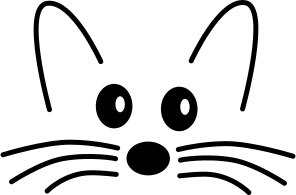
\includegraphics[width=1.4em]{squeak-logo}}}
\iftoshelse{
	\usepackage{marginnote}
		\renewcommand*{\marginfont}{\footnotesize}
	\newcommand{\vartriangleout}{\ifthenelse{\isodd{\thepage}}{\vartriangleright}{\vartriangleleft}}
	\newcommand{\dothisicon}{\fcolorbox{blue!65}{white}{\highlight{$\vartriangleout$}}}
	\newcommand{\dothis}[1]{%
		\noindent\par\noindent
		{\reversemarginpar
			\marginnote{\fcolorbox{blue!65}{white}{\highlight{$\vartriangleout$}}}}
		%\MarginLabel{do this}
		\noindent\emph{#1}
		\nopagebreak}
}{
	\newcommand{\dothisicon}{\raisebox{-.5ex}{
\includegraphics[height=1.2em]{pharo}}}
	\newcommand{\dothis}[1]{%
		\medskip
		\noindent\dothisicon
		\ifx#1\empty\else\quad\emph{#1}\fi
		\par\smallskip\nopagebreak}
}
%===> NEW VERSION <===
% NB: To use this in an individual chapter, you must set:
%\graphicspath{{figures/} {../figures/}}
% at the head of the chapter.  Don't forget the final /
%=============================================================
%:Reader hints (hint)
%
% Indicates a non-obvious consequence
\newcommand{\hint}[1]{\vspace{1ex}\noindent\fbox{\textsc{Hint}} \emph{#1}}
%=================================================================
% graphics for Morphic handles
\newcommand{\grabHandle}{\raisebox{-0.2ex}{
\includegraphics[width=1em]{blackHandle}}}
\newcommand{\moveHandle}{\raisebox{-0.2ex}{
\includegraphics[width=1em]{moveHandle}}}
\newcommand{\debugHandle}{\raisebox{-0.2ex}{
\includegraphics[width=1em]{debugHandle}}}
%=============================================================
%:Highlighting Important stuff (doublebox)
%
% From Seaside book ...
\newsavebox{\SavedText}
\newlength{\InnerBoxRule}\setlength{\InnerBoxRule}{.75\fboxrule}
\newlength{\OuterBoxRule}\setlength{\OuterBoxRule}{1.5\fboxrule}
\newlength{\BoxSeparation}\setlength{\BoxSeparation}{1.5\fboxrule}
\addtolength{\BoxSeparation}{.5pt}
\newlength{\SaveBoxSep}\setlength{\SaveBoxSep}{2\fboxsep}
%
\newenvironment{doublebox}{\begin{lrbox}{\SavedText}
    \begin{minipage}{.75\textwidth}}
    {\end{minipage}\end{lrbox}\begin{center}
    \setlength{\fboxsep}{\BoxSeparation}\setlength{\fboxrule}{\OuterBoxRule}
    \fbox{\setlength{\fboxsep}{\SaveBoxSep}\setlength{\fboxrule}{\InnerBoxRule}%
      \fbox{\usebox{\SavedText}}}
  \end{center}}
% Use this:
\newcommand{\important}[1]{\begin{doublebox}#1\end{doublebox}}
%=============================================================
%:Section depth
\setcounter{secnumdepth}{2}
%% for this to happen start the file with
%\ifx\wholebook\relax\else
%% $Author$
% $Date$
% $Revision$

% HISTORY:
% 2006-10-31 - Oscar code macros
% ...

%=============================================================
% NB: documentclass must be set in main document.
% Allows book to be generated in multiple formats.
%=============================================================
%:Packages
\usepackage[T1]{fontenc}  %%%%%% really important to get the code directly in the text!
\usepackage{lmodern}
%\usepackage[scaled=0.85]{bookmanx} % needs another scale factor if used with \renewcommand{\sfdefault}{cmbr}
\usepackage{palatino}
\usepackage[scaled=0.85]{helvet}
\usepackage[protrusion,expansion=false]{microtype}
\usepackage{graphicx}
\usepackage{theorem}
\usepackage[english]{babel}
% ON: pdfsync breaks the use of p{width} for tabular columns!
\ifdefined\usepdfsync\usepackage{pdfsync}\fi % Requires texlive 2007
%=============================================================
%:More packages
%Stef should check which ones are used!
%\usepackage{picinpar}
%\usepackage{layout}
%\usepackage{color}
%\usepackage{enum}
%\usepackage{a4wide}
% \usepackage{fancyhdr}
\usepackage{ifthen}
\usepackage{float}
\usepackage{longtable}
\usepackage{makeidx}
\usepackage[nottoc]{tocbibind}
\usepackage{multicol}
\usepackage{booktabs}	% book-style tables
\usepackage{topcapt}	% enables \topcaption
\usepackage{multirow}
\usepackage{tabularx}
%\usepackage[bottom]{footmisc}
\usepackage{xspace}
\usepackage{alltt}
\usepackage{amssymb,textcomp}
\usepackage[usenames,dvipsnames]{color}
%\usepackage{colortbl}
\usepackage[hang]{subfigure}\makeatletter\def\p@subfigure{\thefigure\,}\makeatother
\usepackage{rotating}
\usepackage{enumitem}	% apb: allows more control over tags in enumerations
\usepackage{verbatim}     % for comment environment
\usepackage{varioref}	% for page references that work
\labelformat{footnote}{\thechapter--#1} % to distinguish citations from jurabib
\usepackage{needspace}
\usepackage{isodateo} % enable \isodate
\usepackage[newparttoc,pagestyles]{titlesec}
\usepackage{titletoc}
\usepackage{wrapfig}

\usepackage[
	super,
	citefull=first,
	authorformat={allreversed,and},
	titleformat={commasep,italic}
]{jurabib} % citations as footnotes
\usepackage[
	colorlinks=true,
	linkcolor=black,
	urlcolor=black,
	citecolor=black
]{hyperref}   % should come last
%=============================================================
%:PDF version
\pdfminorversion=3 % Set PDF to 1.3 for Lulu
%=============================================================
%:URL style
\makeatletter
\def\url@leostyle{%
  \@ifundefined{selectfont}{\def\UrlFont{\sf}}{\def\UrlFont{\sffamily}}}
\makeatother
% Now actually use the newly defined style.
\urlstyle{leo}
%=============================================================
%:Booleans
\newboolean{lulu}
\setboolean{lulu}{false}
\newcommand{\ifluluelse}[2]{\ifthenelse{\boolean{lulu}}{#1}{#2}}
%=============================================================
%:Names
\newcommand{\SUnit}{SUnit\xspace}
\newcommand{\sunit}{SUnit\xspace}
\newcommand{\xUnit}{$x$Unit\xspace}
\newcommand{\JUnit}{JUnit\xspace}
\newcommand{\st}{Smalltalk\xspace}
\newcommand{\pharo}{Pharo\xspace} % Use this, not \Pharo
%\newcommand{\sqmap}{SqueakMap\xspace}
\newcommand{\squeak}{Squeak\xspace} % use this, not \Squeak or \sq
\newcommand{\sqsrc}{SqueakSource\xspace}
\newcommand{\sbe}{\url{http://SqueakByExample.org}\xspace}
\newcommand{\pharoweb}{\url{http://pharo-project.org}\xspace}
\newcommand{\pbe}{\url{http://PharoByExample.org}\xspace}
\newcommand{\sba}{\url{http://SquareBracketAssociates.org}\xspace}
\newcommand{\bam}{\lct{Bounc\-ing\-Atoms\-Morph}\xspace}
%=============================================================
%:Markup macros for proof-reading
\usepackage[normalem]{ulem} % for \sout
\usepackage{xcolor}
\newcommand{\ra}{$\rightarrow$}
\newcommand{\ugh}[1]{\textcolor{red}{\uwave{#1}}} % please rephrase
\newcommand{\ins}[1]{\textcolor{blue}{\uline{#1}}} % please insert
\newcommand{\del}[1]{\textcolor{red}{\sout{#1}}} % please delete
\newcommand{\chg}[2]{\textcolor{red}{\sout{#1}}{\ra}\textcolor{blue}{\uline{#2}}} % please change
%=============================================================
%:Editorial comment macros
%\newcommand{\nnbb}[2]{
%    % \fbox{\bfseries\sffamily\scriptsize#1}
%    \fcolorbox{gray}{yellow}{\bfseries\sffamily\scriptsize#1}
%    {\sf\small$\blacktriangleright$\textit{#2}$\blacktriangleleft$}
%   }
\newcommand{\yellowbox}[1]{\fcolorbox{gray}{yellow}{\bfseries\sffamily\scriptsize#1}}
\newcommand{\triangles}[1]{{\sf\small$\blacktriangleright$\textit{#1}$\blacktriangleleft$}}
\newcommand{\nnbb}[2]{\yellowbox{#1} \triangles{#2}}
\newcommand{\fix}{\yellowbox{FIX!}}
\newcommand{\here}{\yellowbox{CONTINUE HERE!}}
% editor macros
\newcommand{\apl}[1]{\nnbb{Alain}{#1}} % Alain
\newcommand{\ab}[1]{\nnbb{Andrew}{#1}} % Black
\newcommand{\sd}[1]{\nnbb{St\'{e}f}{#1}} % Ducasse
\newcommand{\gl}[1]{\nnbb{Guillaume}{#1}} % Ducasse
\newcommand{\cd}[1]{\nnbb{Christophe}{#1}} % Ducasse
\newcommand{\sig}[1]{\nnbb{Igor}{#1}} % Igor
\newcommand{\dc}[1]{\nnbb{DamienC}{#1}} % Ducasse
\newcommand{\md}[1]{\nnbb{Marcus}{#1}} % Denker
\newcommand{\on}[1]{\nnbb{Oscar}{#1}} % Nierstrasz
\newcommand{\damien}[1]{\nnbb{Damien}{#1}} % Pollet
\newcommand{\lr}[1]{\nnbb{Lukas}{#1}} % Renggli
\newcommand{\orla}[1]{\nnbb{Orla}{#1}} % Greevy
\newcommand{\alex}[1]{\nnbb{Alex}{#1}} % Bergel
\newcommand{\alx}[1]{\nnbb{Alex}{#1}} % Bergel
\newcommand{\dr}[1]{\nnbb{David}{#1}} % Roethlisberger
\newcommand{\ja}[1]{\nnbb{Jannik}{#1}} % Laval
\newcommand{\cb}[1]{\nnbb{Camillo}{#1}} % Bruni
\newcommand{\jr}[1]{\nnbb{Jorge}{#1}} % Ressia
\newcommand{\jb}[1]{\nnbb{JB}{#1}} % JB
\newcommand{\jp}[1]{\nnbb{Javier}{#1}} % Pimas
\newcommand{\fp}[1]{\nnbb{Fabrizio}{#1}} % Perin
\newcommand{\michael}[1]{\nnbb{Michael}{#1}} % Davies
\newcommand{\ew}[1]{\nnbb{Erwann}{#1}} % Wernli
\newcommand{\mb}[1]{\nnbb{Martial}{#1}} % Boniou
\newcommand{\hw}[1]{\nnbb{Hernan}{#1}} % Wilkinson
\newcommand{\ben}[1]{\nnbb{Benjamin}{#1}} % Benjamin Van Ryseghem
\newcommand{\hjo}[1]{\nnbb{HwaJong}{#1}} % HwaJong Oh aka daliot
\newcommand{\ml}[1]{\nnbb{Max}{#1}} % Max Leske
\newcommand{\mmp}[1]{\nnbb{Mariano}{#1}} % Mariano Martinez Peck
\newcommand{\luc}[1]{\nnbb{Luc}{#1}} % Luc Fabresse
\newcommand{\dkl}[1]{\nnbb{Daniel}{#1}} % Daniel Lyons
\newcommand{\vu}[1]{\nnbb{Veronica}{#1}} % Veronica Uquillas Gomez
\newcommand{\martin}[1]{\nnbb{Martin}{#1}} % Martin Dias
\newcommand{\vp}[1]{\nnbb{Vanessa}{#1}} % Vanessa Pena
\newcommand{\gp}[1]{\nnbb{Guille}{#1}} % Guillermo Polito

%=============================================================
%:Abbreviation macros
\newcommand{\ie}{\emph{i.e.},\xspace}
\newcommand{\eg}{\emph{e.g.},\xspace}
\newcommand{\etc}{etc.\xspace}
%=============================================================
%:Cross reference macros
\newcommand{\charef}[1]{Chapter~\ref{cha:#1}\xspace}
\newcommand{\secref}[1]{Section~\ref{sec:#1}\xspace}
\newcommand{\figref}[1]{Figure~\ref{fig:#1}\xspace}
\newcommand{\Figref}[1]{Figure~\ref{fig:#1}\xspace}
\newcommand{\appref}[1]{Appendix~\ref{app:#1}\xspace}
\newcommand{\tabref}[1]{Table~\ref{tab:#1}\xspace}
\newcommand{\faqref}[1]{FAQ~\ref{faq:#1}, p.~\pageref{faq:#1}\xspace}
% APB: I removed trailing \xspace commands from these macros because
% \xspace mostly doesn't work.  If you want a space after your
% references, type one!
% ON: xspace has always worked just fine for me!  Please leave them in.
%
\newcommand{\ruleref}[1]{\ref{rule:#1}\xspace}
%
\newcommand{\egref}[1]{example~\ref{eg:#1}\xspace}
\newcommand{\Egref}[1]{Example~\ref{eg:#1}\xspace}
%
\newcommand{\scrref}[1]{script~\ref{scr:#1}\xspace}
\newcommand{\Scrref}[1]{Script~\ref{scr:#1}\xspace}
\newcommand{\tscrref}[1]{the script~\ref{scr:#1}\xspace}
\newcommand{\Tscrref}[1]{The script~\ref{scr:#1}\xspace}
%
\newcommand{\mthref}[1]{method~\ref{mth:#1}\xspace}
\newcommand{\mthsref}[1]{methods~\ref{mth:#1}\xspace}
\newcommand{\Mthref}[1]{Method~\ref{mth:#1}\xspace}
\newcommand{\tmthref}[1]{the method~\ref{mth:#1}\xspace}
\newcommand{\Tmthref}[1]{The method~\ref{mth:#1}\xspace}
%
\newcommand{\clsref}[1]{class~\ref{cls:#1}\xspace}
\newcommand{\tclsref}[1]{the class~\ref{cls:#1}\xspace}
\newcommand{\Tclsref}[1]{The class~\ref{cls:#1}\xspace}

\newcommand{\chalabel}[1]{\label{cha:#1}}
\newcommand{\seclabel}[1]{\label{sec:#1}}
\newcommand{\figlabel}[1]{\label{fig:#1}}
\newcommand{\tablabel}[1]{\label{tab:#1}}
\newcommand{\rulelabel}[1]{\label{rule:#1}}
\newcommand{\eglabel}[1]{\label{eg:#1}}
\newcommand{\scrlabel}[1]{\label{scr:#1}}
\newcommand{\mthlabel}[1]{\label{mth:#1}}
\newcommand{\clslabel}[1]{\label{cls:#1}}
\newcommand{\faqlabel}[1]{\label{faq:#1}}
%=============================================================
%:Menu item macro
% for menu items, so we can change our minds on how to print them! (apb)
\definecolor{lightgray}{gray}{0.89}
\newcommand{\menu}[1]{{%
	\setlength{\fboxsep}{0pt}%
	\colorbox{lightgray}{{{\upshape\sffamily\strut \,#1\,}}}}}
\newcommand{\link}[1]{{%
	\fontfamily{lmr}\selectfont
 	\upshape{\sffamily \underline{#1}}}}
% For submenu items:
\newcommand{\go}{\,$\triangleright$\,}
% \newcommand{\go}{\,$\blacktriangleright$\,}
% For keyboard shortcuts:
%\newcommand{\short}[1]{\mbox{$\langle${\sc CMD}$\rangle$-#1}\xspace}
\newcommand{\short}[1]{\mbox{{\sc cmd}\hspace{0.08em}--\hspace{0.09em}#1}\xspace}
% For buttons:
\newcommand{\button}[1]{{%
	\setlength{\fboxsep}{0pt}%
	\fbox{{\upshape\sffamily\strut \,#1\,}}}}
% NB: The button macro does not work within captions -- incompatible with xcolor package :-(
\newcommand{\toolsflap}{\textit{Tools} flap\xspace}
%=============================================================
%:Mouse clicks
\newcommand{\click}{click\xspace} % RED
\newcommand{\actclick}{action-click\xspace} % YELLOW
\newcommand{\metaclick}{meta-click\xspace} % BLUE
\newcommand{\Click}{Click\xspace} % RED
\newcommand{\Actclick}{Action-click\xspace} % YELLOW
\newcommand{\Metaclick}{Meta-click\xspace} % BLUE
%=============================================================
%:ToSh macros
\newboolean{tosh}
\setboolean{tosh}{false}
\newcommand{\iftoshelse}[2]{\ifthenelse{\boolean{tosh}}{#1}{#2}}
%=============================================================
%:ToSh colors
%\newcommand{\highlightcolor}{\color{blue!65}}
%\newcommand{\boxcolor}{\color{gray!25}}
\newcommand{\highlight}[1]{\textcolor{blue!65}{#1}}
%\newcommand{\codecolor}{\color{blue!65}}
%%\setlength{\fboxrule}{2pt}
%\newcommand{\asPict}[1]{%
%	{\Large\highlight{#1}}}
%=============================================================
%:Reader cues (do this)
%
% Indicate something the reader should try out.
% \newcommand{\dothisicon}{\raisebox{-.5ex}{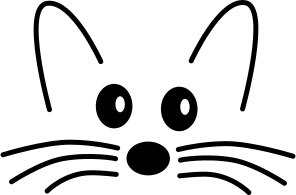
\includegraphics[width=1.4em]{squeak-logo}}}
\iftoshelse{
	\usepackage{marginnote}
		\renewcommand*{\marginfont}{\footnotesize}
	\newcommand{\vartriangleout}{\ifthenelse{\isodd{\thepage}}{\vartriangleright}{\vartriangleleft}}
	\newcommand{\dothisicon}{\fcolorbox{blue!65}{white}{\highlight{$\vartriangleout$}}}
	\newcommand{\dothis}[1]{%
		\noindent\par\noindent
		{\reversemarginpar
			\marginnote{\fcolorbox{blue!65}{white}{\highlight{$\vartriangleout$}}}}
		%\MarginLabel{do this}
		\noindent\emph{#1}
		\nopagebreak}
}{
	\newcommand{\dothisicon}{\raisebox{-.5ex}{
\includegraphics[height=1.2em]{pharo}}}
	\newcommand{\dothis}[1]{%
		\medskip
		\noindent\dothisicon
		\ifx#1\empty\else\quad\emph{#1}\fi
		\par\smallskip\nopagebreak}
}
%===> NEW VERSION <===
% NB: To use this in an individual chapter, you must set:
%\graphicspath{{figures/} {../figures/}}
% at the head of the chapter.  Don't forget the final /
%=============================================================
%:Reader hints (hint)
%
% Indicates a non-obvious consequence
\newcommand{\hint}[1]{\vspace{1ex}\noindent\fbox{\textsc{Hint}} \emph{#1}}
%=================================================================
% graphics for Morphic handles
\newcommand{\grabHandle}{\raisebox{-0.2ex}{
\includegraphics[width=1em]{blackHandle}}}
\newcommand{\moveHandle}{\raisebox{-0.2ex}{
\includegraphics[width=1em]{moveHandle}}}
\newcommand{\debugHandle}{\raisebox{-0.2ex}{
\includegraphics[width=1em]{debugHandle}}}
%=============================================================
%:Highlighting Important stuff (doublebox)
%
% From Seaside book ...
\newsavebox{\SavedText}
\newlength{\InnerBoxRule}\setlength{\InnerBoxRule}{.75\fboxrule}
\newlength{\OuterBoxRule}\setlength{\OuterBoxRule}{1.5\fboxrule}
\newlength{\BoxSeparation}\setlength{\BoxSeparation}{1.5\fboxrule}
\addtolength{\BoxSeparation}{.5pt}
\newlength{\SaveBoxSep}\setlength{\SaveBoxSep}{2\fboxsep}
%
\newenvironment{doublebox}{\begin{lrbox}{\SavedText}
    \begin{minipage}{.75\textwidth}}
    {\end{minipage}\end{lrbox}\begin{center}
    \setlength{\fboxsep}{\BoxSeparation}\setlength{\fboxrule}{\OuterBoxRule}
    \fbox{\setlength{\fboxsep}{\SaveBoxSep}\setlength{\fboxrule}{\InnerBoxRule}%
      \fbox{\usebox{\SavedText}}}
  \end{center}}
% Use this:
\newcommand{\important}[1]{\begin{doublebox}#1\end{doublebox}}
%=============================================================
%:Section depth
\setcounter{secnumdepth}{2}
%% for this to happen start the file with
%\ifx\wholebook\relax\else
%% $Author$
% $Date$
% $Revision$

% HISTORY:
% 2006-10-31 - Oscar code macros
% ...

%=============================================================
% NB: documentclass must be set in main document.
% Allows book to be generated in multiple formats.
%=============================================================
%:Packages
\usepackage[T1]{fontenc}  %%%%%% really important to get the code directly in the text!
\usepackage{lmodern}
%\usepackage[scaled=0.85]{bookmanx} % needs another scale factor if used with \renewcommand{\sfdefault}{cmbr}
\usepackage{palatino}
\usepackage[scaled=0.85]{helvet}
\usepackage[protrusion,expansion=false]{microtype}
\usepackage{graphicx}
\usepackage{theorem}
\usepackage[english]{babel}
% ON: pdfsync breaks the use of p{width} for tabular columns!
\ifdefined\usepdfsync\usepackage{pdfsync}\fi % Requires texlive 2007
%=============================================================
%:More packages
%Stef should check which ones are used!
%\usepackage{picinpar}
%\usepackage{layout}
%\usepackage{color}
%\usepackage{enum}
%\usepackage{a4wide}
% \usepackage{fancyhdr}
\usepackage{ifthen}
\usepackage{float}
\usepackage{longtable}
\usepackage{makeidx}
\usepackage[nottoc]{tocbibind}
\usepackage{multicol}
\usepackage{booktabs}	% book-style tables
\usepackage{topcapt}	% enables \topcaption
\usepackage{multirow}
\usepackage{tabularx}
%\usepackage[bottom]{footmisc}
\usepackage{xspace}
\usepackage{alltt}
\usepackage{amssymb,textcomp}
\usepackage[usenames,dvipsnames]{color}
%\usepackage{colortbl}
\usepackage[hang]{subfigure}\makeatletter\def\p@subfigure{\thefigure\,}\makeatother
\usepackage{rotating}
\usepackage{enumitem}	% apb: allows more control over tags in enumerations
\usepackage{verbatim}     % for comment environment
\usepackage{varioref}	% for page references that work
\labelformat{footnote}{\thechapter--#1} % to distinguish citations from jurabib
\usepackage{needspace}
\usepackage{isodateo} % enable \isodate
\usepackage[newparttoc,pagestyles]{titlesec}
\usepackage{titletoc}
\usepackage{wrapfig}

\usepackage[
	super,
	citefull=first,
	authorformat={allreversed,and},
	titleformat={commasep,italic}
]{jurabib} % citations as footnotes
\usepackage[
	colorlinks=true,
	linkcolor=black,
	urlcolor=black,
	citecolor=black
]{hyperref}   % should come last
%=============================================================
%:PDF version
\pdfminorversion=3 % Set PDF to 1.3 for Lulu
%=============================================================
%:URL style
\makeatletter
\def\url@leostyle{%
  \@ifundefined{selectfont}{\def\UrlFont{\sf}}{\def\UrlFont{\sffamily}}}
\makeatother
% Now actually use the newly defined style.
\urlstyle{leo}
%=============================================================
%:Booleans
\newboolean{lulu}
\setboolean{lulu}{false}
\newcommand{\ifluluelse}[2]{\ifthenelse{\boolean{lulu}}{#1}{#2}}
%=============================================================
%:Names
\newcommand{\SUnit}{SUnit\xspace}
\newcommand{\sunit}{SUnit\xspace}
\newcommand{\xUnit}{$x$Unit\xspace}
\newcommand{\JUnit}{JUnit\xspace}
\newcommand{\st}{Smalltalk\xspace}
\newcommand{\pharo}{Pharo\xspace} % Use this, not \Pharo
%\newcommand{\sqmap}{SqueakMap\xspace}
\newcommand{\squeak}{Squeak\xspace} % use this, not \Squeak or \sq
\newcommand{\sqsrc}{SqueakSource\xspace}
\newcommand{\sbe}{\url{http://SqueakByExample.org}\xspace}
\newcommand{\pharoweb}{\url{http://pharo-project.org}\xspace}
\newcommand{\pbe}{\url{http://PharoByExample.org}\xspace}
\newcommand{\sba}{\url{http://SquareBracketAssociates.org}\xspace}
\newcommand{\bam}{\lct{Bounc\-ing\-Atoms\-Morph}\xspace}
%=============================================================
%:Markup macros for proof-reading
\usepackage[normalem]{ulem} % for \sout
\usepackage{xcolor}
\newcommand{\ra}{$\rightarrow$}
\newcommand{\ugh}[1]{\textcolor{red}{\uwave{#1}}} % please rephrase
\newcommand{\ins}[1]{\textcolor{blue}{\uline{#1}}} % please insert
\newcommand{\del}[1]{\textcolor{red}{\sout{#1}}} % please delete
\newcommand{\chg}[2]{\textcolor{red}{\sout{#1}}{\ra}\textcolor{blue}{\uline{#2}}} % please change
%=============================================================
%:Editorial comment macros
%\newcommand{\nnbb}[2]{
%    % \fbox{\bfseries\sffamily\scriptsize#1}
%    \fcolorbox{gray}{yellow}{\bfseries\sffamily\scriptsize#1}
%    {\sf\small$\blacktriangleright$\textit{#2}$\blacktriangleleft$}
%   }
\newcommand{\yellowbox}[1]{\fcolorbox{gray}{yellow}{\bfseries\sffamily\scriptsize#1}}
\newcommand{\triangles}[1]{{\sf\small$\blacktriangleright$\textit{#1}$\blacktriangleleft$}}
\newcommand{\nnbb}[2]{\yellowbox{#1} \triangles{#2}}
\newcommand{\fix}{\yellowbox{FIX!}}
\newcommand{\here}{\yellowbox{CONTINUE HERE!}}
% editor macros
\newcommand{\apl}[1]{\nnbb{Alain}{#1}} % Alain
\newcommand{\ab}[1]{\nnbb{Andrew}{#1}} % Black
\newcommand{\sd}[1]{\nnbb{St\'{e}f}{#1}} % Ducasse
\newcommand{\gl}[1]{\nnbb{Guillaume}{#1}} % Ducasse
\newcommand{\cd}[1]{\nnbb{Christophe}{#1}} % Ducasse
\newcommand{\sig}[1]{\nnbb{Igor}{#1}} % Igor
\newcommand{\dc}[1]{\nnbb{DamienC}{#1}} % Ducasse
\newcommand{\md}[1]{\nnbb{Marcus}{#1}} % Denker
\newcommand{\on}[1]{\nnbb{Oscar}{#1}} % Nierstrasz
\newcommand{\damien}[1]{\nnbb{Damien}{#1}} % Pollet
\newcommand{\lr}[1]{\nnbb{Lukas}{#1}} % Renggli
\newcommand{\orla}[1]{\nnbb{Orla}{#1}} % Greevy
\newcommand{\alex}[1]{\nnbb{Alex}{#1}} % Bergel
\newcommand{\alx}[1]{\nnbb{Alex}{#1}} % Bergel
\newcommand{\dr}[1]{\nnbb{David}{#1}} % Roethlisberger
\newcommand{\ja}[1]{\nnbb{Jannik}{#1}} % Laval
\newcommand{\cb}[1]{\nnbb{Camillo}{#1}} % Bruni
\newcommand{\jr}[1]{\nnbb{Jorge}{#1}} % Ressia
\newcommand{\jb}[1]{\nnbb{JB}{#1}} % JB
\newcommand{\jp}[1]{\nnbb{Javier}{#1}} % Pimas
\newcommand{\fp}[1]{\nnbb{Fabrizio}{#1}} % Perin
\newcommand{\michael}[1]{\nnbb{Michael}{#1}} % Davies
\newcommand{\ew}[1]{\nnbb{Erwann}{#1}} % Wernli
\newcommand{\mb}[1]{\nnbb{Martial}{#1}} % Boniou
\newcommand{\hw}[1]{\nnbb{Hernan}{#1}} % Wilkinson
\newcommand{\ben}[1]{\nnbb{Benjamin}{#1}} % Benjamin Van Ryseghem
\newcommand{\hjo}[1]{\nnbb{HwaJong}{#1}} % HwaJong Oh aka daliot
\newcommand{\ml}[1]{\nnbb{Max}{#1}} % Max Leske
\newcommand{\mmp}[1]{\nnbb{Mariano}{#1}} % Mariano Martinez Peck
\newcommand{\luc}[1]{\nnbb{Luc}{#1}} % Luc Fabresse
\newcommand{\dkl}[1]{\nnbb{Daniel}{#1}} % Daniel Lyons
\newcommand{\vu}[1]{\nnbb{Veronica}{#1}} % Veronica Uquillas Gomez
\newcommand{\martin}[1]{\nnbb{Martin}{#1}} % Martin Dias
\newcommand{\vp}[1]{\nnbb{Vanessa}{#1}} % Vanessa Pena
\newcommand{\gp}[1]{\nnbb{Guille}{#1}} % Guillermo Polito

%=============================================================
%:Abbreviation macros
\newcommand{\ie}{\emph{i.e.},\xspace}
\newcommand{\eg}{\emph{e.g.},\xspace}
\newcommand{\etc}{etc.\xspace}
%=============================================================
%:Cross reference macros
\newcommand{\charef}[1]{Chapter~\ref{cha:#1}\xspace}
\newcommand{\secref}[1]{Section~\ref{sec:#1}\xspace}
\newcommand{\figref}[1]{Figure~\ref{fig:#1}\xspace}
\newcommand{\Figref}[1]{Figure~\ref{fig:#1}\xspace}
\newcommand{\appref}[1]{Appendix~\ref{app:#1}\xspace}
\newcommand{\tabref}[1]{Table~\ref{tab:#1}\xspace}
\newcommand{\faqref}[1]{FAQ~\ref{faq:#1}, p.~\pageref{faq:#1}\xspace}
% APB: I removed trailing \xspace commands from these macros because
% \xspace mostly doesn't work.  If you want a space after your
% references, type one!
% ON: xspace has always worked just fine for me!  Please leave them in.
%
\newcommand{\ruleref}[1]{\ref{rule:#1}\xspace}
%
\newcommand{\egref}[1]{example~\ref{eg:#1}\xspace}
\newcommand{\Egref}[1]{Example~\ref{eg:#1}\xspace}
%
\newcommand{\scrref}[1]{script~\ref{scr:#1}\xspace}
\newcommand{\Scrref}[1]{Script~\ref{scr:#1}\xspace}
\newcommand{\tscrref}[1]{the script~\ref{scr:#1}\xspace}
\newcommand{\Tscrref}[1]{The script~\ref{scr:#1}\xspace}
%
\newcommand{\mthref}[1]{method~\ref{mth:#1}\xspace}
\newcommand{\mthsref}[1]{methods~\ref{mth:#1}\xspace}
\newcommand{\Mthref}[1]{Method~\ref{mth:#1}\xspace}
\newcommand{\tmthref}[1]{the method~\ref{mth:#1}\xspace}
\newcommand{\Tmthref}[1]{The method~\ref{mth:#1}\xspace}
%
\newcommand{\clsref}[1]{class~\ref{cls:#1}\xspace}
\newcommand{\tclsref}[1]{the class~\ref{cls:#1}\xspace}
\newcommand{\Tclsref}[1]{The class~\ref{cls:#1}\xspace}

\newcommand{\chalabel}[1]{\label{cha:#1}}
\newcommand{\seclabel}[1]{\label{sec:#1}}
\newcommand{\figlabel}[1]{\label{fig:#1}}
\newcommand{\tablabel}[1]{\label{tab:#1}}
\newcommand{\rulelabel}[1]{\label{rule:#1}}
\newcommand{\eglabel}[1]{\label{eg:#1}}
\newcommand{\scrlabel}[1]{\label{scr:#1}}
\newcommand{\mthlabel}[1]{\label{mth:#1}}
\newcommand{\clslabel}[1]{\label{cls:#1}}
\newcommand{\faqlabel}[1]{\label{faq:#1}}
%=============================================================
%:Menu item macro
% for menu items, so we can change our minds on how to print them! (apb)
\definecolor{lightgray}{gray}{0.89}
\newcommand{\menu}[1]{{%
	\setlength{\fboxsep}{0pt}%
	\colorbox{lightgray}{{{\upshape\sffamily\strut \,#1\,}}}}}
\newcommand{\link}[1]{{%
	\fontfamily{lmr}\selectfont
 	\upshape{\sffamily \underline{#1}}}}
% For submenu items:
\newcommand{\go}{\,$\triangleright$\,}
% \newcommand{\go}{\,$\blacktriangleright$\,}
% For keyboard shortcuts:
%\newcommand{\short}[1]{\mbox{$\langle${\sc CMD}$\rangle$-#1}\xspace}
\newcommand{\short}[1]{\mbox{{\sc cmd}\hspace{0.08em}--\hspace{0.09em}#1}\xspace}
% For buttons:
\newcommand{\button}[1]{{%
	\setlength{\fboxsep}{0pt}%
	\fbox{{\upshape\sffamily\strut \,#1\,}}}}
% NB: The button macro does not work within captions -- incompatible with xcolor package :-(
\newcommand{\toolsflap}{\textit{Tools} flap\xspace}
%=============================================================
%:Mouse clicks
\newcommand{\click}{click\xspace} % RED
\newcommand{\actclick}{action-click\xspace} % YELLOW
\newcommand{\metaclick}{meta-click\xspace} % BLUE
\newcommand{\Click}{Click\xspace} % RED
\newcommand{\Actclick}{Action-click\xspace} % YELLOW
\newcommand{\Metaclick}{Meta-click\xspace} % BLUE
%=============================================================
%:ToSh macros
\newboolean{tosh}
\setboolean{tosh}{false}
\newcommand{\iftoshelse}[2]{\ifthenelse{\boolean{tosh}}{#1}{#2}}
%=============================================================
%:ToSh colors
%\newcommand{\highlightcolor}{\color{blue!65}}
%\newcommand{\boxcolor}{\color{gray!25}}
\newcommand{\highlight}[1]{\textcolor{blue!65}{#1}}
%\newcommand{\codecolor}{\color{blue!65}}
%%\setlength{\fboxrule}{2pt}
%\newcommand{\asPict}[1]{%
%	{\Large\highlight{#1}}}
%=============================================================
%:Reader cues (do this)
%
% Indicate something the reader should try out.
% \newcommand{\dothisicon}{\raisebox{-.5ex}{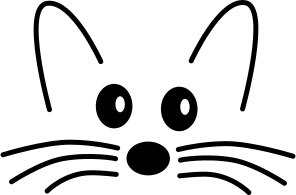
\includegraphics[width=1.4em]{squeak-logo}}}
\iftoshelse{
	\usepackage{marginnote}
		\renewcommand*{\marginfont}{\footnotesize}
	\newcommand{\vartriangleout}{\ifthenelse{\isodd{\thepage}}{\vartriangleright}{\vartriangleleft}}
	\newcommand{\dothisicon}{\fcolorbox{blue!65}{white}{\highlight{$\vartriangleout$}}}
	\newcommand{\dothis}[1]{%
		\noindent\par\noindent
		{\reversemarginpar
			\marginnote{\fcolorbox{blue!65}{white}{\highlight{$\vartriangleout$}}}}
		%\MarginLabel{do this}
		\noindent\emph{#1}
		\nopagebreak}
}{
	\newcommand{\dothisicon}{\raisebox{-.5ex}{
\includegraphics[height=1.2em]{pharo}}}
	\newcommand{\dothis}[1]{%
		\medskip
		\noindent\dothisicon
		\ifx#1\empty\else\quad\emph{#1}\fi
		\par\smallskip\nopagebreak}
}
%===> NEW VERSION <===
% NB: To use this in an individual chapter, you must set:
%\graphicspath{{figures/} {../figures/}}
% at the head of the chapter.  Don't forget the final /
%=============================================================
%:Reader hints (hint)
%
% Indicates a non-obvious consequence
\newcommand{\hint}[1]{\vspace{1ex}\noindent\fbox{\textsc{Hint}} \emph{#1}}
%=================================================================
% graphics for Morphic handles
\newcommand{\grabHandle}{\raisebox{-0.2ex}{
\includegraphics[width=1em]{blackHandle}}}
\newcommand{\moveHandle}{\raisebox{-0.2ex}{
\includegraphics[width=1em]{moveHandle}}}
\newcommand{\debugHandle}{\raisebox{-0.2ex}{
\includegraphics[width=1em]{debugHandle}}}
%=============================================================
%:Highlighting Important stuff (doublebox)
%
% From Seaside book ...
\newsavebox{\SavedText}
\newlength{\InnerBoxRule}\setlength{\InnerBoxRule}{.75\fboxrule}
\newlength{\OuterBoxRule}\setlength{\OuterBoxRule}{1.5\fboxrule}
\newlength{\BoxSeparation}\setlength{\BoxSeparation}{1.5\fboxrule}
\addtolength{\BoxSeparation}{.5pt}
\newlength{\SaveBoxSep}\setlength{\SaveBoxSep}{2\fboxsep}
%
\newenvironment{doublebox}{\begin{lrbox}{\SavedText}
    \begin{minipage}{.75\textwidth}}
    {\end{minipage}\end{lrbox}\begin{center}
    \setlength{\fboxsep}{\BoxSeparation}\setlength{\fboxrule}{\OuterBoxRule}
    \fbox{\setlength{\fboxsep}{\SaveBoxSep}\setlength{\fboxrule}{\InnerBoxRule}%
      \fbox{\usebox{\SavedText}}}
  \end{center}}
% Use this:
\newcommand{\important}[1]{\begin{doublebox}#1\end{doublebox}}
%=============================================================
%:Section depth
\setcounter{secnumdepth}{2}
%% for this to happen start the file with
%\ifx\wholebook\relax\else
%\input{../common.tex}
%\begin{document}
%\fi
% and terminate by
% \ifx\wholebook\relax\else\end{document}\fi

\DeclareGraphicsExtensions{.pdf, .jpg, .png}
%=============================================================
%:PDF setup
\hypersetup{
%   a4paper,
%   pdfstartview=FitV,
%   colorlinks,
%   linkcolor=darkblue,
%   citecolor=darkblue,
   pdftitle={Pharo by Example},
   pdfauthor={Andrew P. Black, St\'ephane Ducasse,	Oscar Nierstrasz,
Damien Pollet},
   pdfkeywords={Smalltalk, Squeak, Object-Oriented Programming, OOP},
   pdfsubject={Computer Science}
}
%=============================================================
%:Page layout and appearance
%
% \renewcommand{\headrulewidth}{0pt}
\renewcommand{\chaptermark}[1]{\markboth{#1}{}}
\renewcommand{\sectionmark}[1]{\markright{\thesection\ #1}}
\renewpagestyle{plain}[\small\itshape]{%
	\setheadrule{0pt}%
	\sethead[][][]{}{}{}%
	\setfoot[][][]{}{}{}}
\renewpagestyle{headings}[\small\itshape]{%
	\setheadrule{0pt}%
	\setmarks{chapter}{section}%
	\sethead[\thepage][][\chaptertitle]{\sectiontitle}{}{\thepage}%
	\setfoot[][][]{}{}{}}
%=============================================================
%:Title section setup and TOC numbering depth
\setcounter{secnumdepth}{1}
\setcounter{tocdepth}{1}
\titleformat{\part}[display]{\centering}{\huge\partname\ \thepart}{1em}{\Huge\textbf}[]
\titleformat{\chapter}[display]{}{\huge\chaptertitlename\ \thechapter}{1em}{\Huge\raggedright\textbf}[]
\titlecontents{part}[3pc]{%
		\pagebreak[2]\addvspace{1em plus.4em minus.2em}%
		\leavevmode\large\bfseries}
	{\contentslabel{3pc}}{\hspace*{-3pc}}
	{}[\nopagebreak]
\titlecontents{chapter}[3pc]{%
		\pagebreak[0]\addvspace{1em plus.2em minus.2em}%
		\leavevmode\bfseries}
	{\contentslabel{3pc}}{}
	{\hfill\contentspage}[\nopagebreak]
\dottedcontents{section}[3pc]{}{3pc}{1pc}
\dottedcontents{subsection}[3pc]{}{0pc}{1pc}
% \dottedcontents{subsection}[4.5em]{}{0pt}{1pc}
% Make \cleardoublepage insert really blank pages http://www.tex.ac.uk/cgi-bin/texfaq2html?label=reallyblank
\let\origdoublepage\cleardoublepage
\newcommand{\clearemptydoublepage}{%
  \clearpage
  {\pagestyle{empty}\origdoublepage}}
\let\cleardoublepage\clearemptydoublepage % see http://www.tex.ac.uk/cgi-bin/texfaq2html?label=patch
%=============================================================
%:FAQ macros (for FAQ chapter)
\newtheorem{faq}{FAQ}
\newcommand{\answer}{\paragraph{Answer}\ }
%=============================================================
%:Listings package configuration
% \newcommand{\caret}{\makebox{\raisebox{0.4ex}{\footnotesize{$\wedge$}}}}
\newcommand{\caret}{\^\,}
\newcommand{\escape}{{\sf \textbackslash}}
\definecolor{source}{gray}{0.95}
\usepackage{listings}
\lstdefinelanguage{Smalltalk}{
%  morekeywords={self,super,true,false,nil,thisContext}, % This is overkill
  morestring=[d]',
  morecomment=[s]{"}{"},
  alsoletter={\#:},
  escapechar={!},
  literate=
    {BANG}{!}1
    {CARET}{\^}1
    {UNDERSCORE}{\_}1
    {\\st}{Smalltalk}9 % convenience -- in case \st occurs in code
    % {'}{{\textquotesingle}}1 % replaced by upquote=true in \lstset
    %{_}{{$\leftarrow$}}1
    {>>>}{{\sep}}1
    %{^}{{$\uparrow$}}1
    {~}{{$\sim$}}1
    {-}{{\texttt{-}}}1 %{\textminus}}1 %{-}{\hspace{-0.13em}}{-}}1  % the goal is to make - the same width as +
    % {+}{\sf+}1 %{\raisebox{0.08ex}{+}}}1      % and to raise + off the baseline to match -
    {-->}{{\quad$\longrightarrow$\quad}}3
    {~->}{{\quad$\leadsto$\quad}}3
	, % Don't forget the comma at the end!
  tabsize=4
}[keywords,comments,strings]

\lstset{language=Smalltalk,
	basicstyle=\sffamily,
	keywordstyle=\color{black}\bfseries,
	% stringstyle=\ttfamily, % Ugly! do we really want this? -- on
	mathescape=true,
	showstringspaces=false,
	keepspaces=true,
	breaklines=true,
	breakautoindent=true,
	backgroundcolor=\color{source},
	lineskip={-1pt}, % Ugly hack
	upquote=true, % straight quote; requires textcomp package
	columns=fullflexible} % no fixed width fonts
% In-line code (literal)
% Normally use this for all in-line code:

\newcommand{\ct}{\lstinline[mathescape=false,backgroundcolor=\color{white},basicstyle={\sffamily\upshape}]}
\newcommand{\cts}[1]{{\sffamily{\upshape{#1}}\xspace}}
% apb 2007.8.28 added the \upshape declaration to avoid getting italicized code in \dothis{ } sections.
% In-line code (latex enabled)
% Use this only in special situations where \ct does not work
% (within section headings ...):
\newcommand{\lct}[1]{{\textsf{\textup{#1}}}}
% Use these for system categories and protocols:
\newcommand{\scat}[1]{\emph{\textsf{#1}}\xspace}
\newcommand{\pkg}[1]{\emph{\textsf{#1}}\xspace}
\newcommand{\prot}[1]{\emph{\textsf{#1}}\xspace}
% Code environments
% NB: the arg is for tests
% Only code and example environments may be tests
\lstnewenvironment{code}[1]{%
	\lstset{%
		% frame=lines,
		frame=single,
		framerule=0pt,
		mathescape=false
	}
}{}
\def\ignoredollar#1{}
%=============================================================
%:Code environments (method, script ...)
% NB: the third arg is for tests
% Only code and example environments may be tests
\lstnewenvironment{example}[3][defaultlabel]{%
	\renewcommand{\lstlistingname}{Example}%
	\lstset{
		% frame=lines,
		frame=single,
		framerule=0pt,
		mathescape=false,
		caption={\emph{#2}},
		label={eg:#1}
	}
}{}
\lstnewenvironment{script}[2][defaultlabel]{%
\renewcommand{\lstlistingname}{Script}%
	\lstset{
		% frame=lines,
		frame=single,
		framerule=0pt,
		mathescape=false,
		name={Script},
		caption={\emph{#2}},
		label={scr:#1}
	}
}{}
\lstnewenvironment{method}[2][defaultlabel]{%
	\renewcommand{\lstlistingname}{Method}%
	\lstset{
		% frame=lines,
		frame=single,
		framerule=0pt,
		mathescape=false,
		name={Method},
		caption={\emph{#2}},
		label={mth:#1}
	}
}{}
\lstnewenvironment{methods}[2][defaultlabel]{% just for multiple methods at once
	\renewcommand{\lstlistingname}{Methods}%
	\lstset{
		% frame=lines,
		frame=single,
		framerule=0pt,
		mathescape=false,
		name={Method},
		caption={\emph{#2}},
		label={mth:#1}
	}
}{}
\lstnewenvironment{numMethod}[2][defaultlabel]{%
	\renewcommand{\lstlistingname}{Method}%
	\lstset{
		numbers=left,
		numberstyle={\tiny\sffamily},
		% frame=lines,
		frame=single,
		framerule=0pt,
		mathescape=false,
		name={Method},
		caption={\emph{#2}},
		label={mth:#1}
	}
}{}
\lstnewenvironment{classdef}[2][defaultlabel]{%
	\renewcommand{\lstlistingname}{Class}%
	\lstset{
		% frame=lines,
		frame=single,
		framerule=0pt,
		mathescape=false,
		name={Class},
		caption={\emph{#2}},
		label={cls:#1}
	}
}{}
%=============================================================
%:Reserving space
% Usually need one more line than the actual lines of code
\newcommand{\needlines}[1]{\Needspace{#1\baselineskip}}
%=============================================================
%:Indexing macros
% Macros ending with "ind" generate text as well as an index entry
% Macros ending with "index" *only* generate an index entry
\newcommand{\ind}[1]{\index{#1}#1\xspace} % plain text
\newcommand{\subind}[2]{\index{#1!#2}#2\xspace} % show #2, subindex under #1
\newcommand{\emphind}[1]{\index{#1}\emph{#1}\xspace} % emph #1
\newcommand{\emphsubind}[2]{\index{#1!#2}\emph{#2}\xspace} % show emph #2, subindex inder #1
\newcommand{\scatind}[1]{\index{#1@\textsf{#1} (category)}\scat{#1}} % category
\newcommand{\pkgind}[1]{\index{#1@\textsf{#1} (package)}\pkg{#1}} % package
\newcommand{\protind}[1]{\index{#1@\textsf{#1} (protocol)}\prot{#1}} % protocol
\newcommand{\clsind}[1]{\index{#1@\textsf{#1} (class)}\ct{#1}\xspace}
% \newcommand{\clsind}[1]{\index{#1!\#@(class)}\ct{#1}\xspace} % class
\newcommand{\clsindplural}[1]{\index{#1!\#@(class)}\ct{#1}s\xspace} % class
\newcommand{\cvind}[1]{\index{#1@\textsf{#1} (class variable)}\ct{#1}\xspace} % class var
\newcommand{\glbind}[1]{\index{#1@\textsf{#1} (global)}\ct{#1}\xspace} % global
\newcommand{\patind}[1]{\index{#1@#1 (pattern)}\ct{#1}\xspace} % pattern
\newcommand{\pvind}[1]{\index{#1@\textsf{#1} (pseudo variable)}\ct{#1}\xspace} % pseudo var
\newcommand{\clsmthind}[2]{\index{#1!#2@\ct{#2}}\ct{#1>>>#2}\xspace} % class + method name
\newcommand{\mthind}[2]{\index{#1!#2@\ct{#2}}\ct{#2}\xspace} % show method name only
\newcommand{\lmthind}[2]{\index{#1!#2@\ct{#2}}\lct{#2}\xspace} % show method name only
\newcommand{\cmind}[2]{\index{#1!#2@\ct{#2}}\ct{#1>>>#2}\xspace} % show class>>method
\newcommand{\lcmind}[2]{\index{#1!#2@\ct{#2}}\lct{#1>>>#2}\xspace} % show class>>method
\newcommand{\toolsflapind}{\index{Tools flap}\toolsflap} % index tools flap
% The following only generate an index entry:
% \newcommand{\clsindex}[1]{\index{#1@\textsf{#1} (class)}}
\newcommand{\clsindex}[1]{\index{#1!\#@(class)}} % class
\newcommand{\mthindex}[2]{\index{#1!#2@\ct{#2}}} % method
\newcommand{\cmindex}[2]{\index{#1!#2@\ct{#2}}} % class>>method
\newcommand{\cvindex}[1]{\index{#1@\textsf{#1} (class variable)}} % class var
\newcommand{\glbindex}[1]{\index{#1@\textsf{#1} (global)}}% global
\newcommand{\pvindex}[1]{\index{#1@\textsf{#1} (pseudo variable)}}% pseudo var
\newcommand{\seeindex}[2]{\index{#1|see{#2}}} % #1, see #2
\newcommand{\scatindex}[1]{\index{#1@\textsf{#1} (category)}} % category
\newcommand{\pkgindex}[1]{\index{#1@\textsf{#1} (package)}} % package
\newcommand{\protindex}[1]{\index{#1@\textsf{#1} (protocol)}} % protocol
% How can we have the main entry page numbers in bold yet not break the hyperlink?
\newcommand{\boldidx}[1]{{\bf #1}} % breaks hyperlink
%\newcommand{\indmain}[1]{\index{#1|boldidx}#1\xspace} % plain text, main entry
%\newcommand{\emphsubindmain}[2]{\index{#1!#2|boldidx}\emph{#2}\xspace} % subindex, main entry
%\newcommand{\subindmain}[2]{\index{#1!#2|boldidx}#2\xspace} % subindex, main entry
%\newcommand{\clsindmain}[1]{\index{#1@\textsf{#1} (class)|boldidx}\ct{#1}\xspace}
%\newcommand{\clsindmain}[1]{\index{#1!\#@(class)|boldidx}\ct{#1}\xspace} % class main
%\newcommand{\indexmain}[1]{\index{#1|boldidx}} % main index entry only
\newcommand{\indmain}[1]{\index{#1}#1\xspace} % The main index entry for this item
\newcommand{\emphsubindmain}[2]{\index{#1!#2}\emph{#2}\xspace} % subindex, main entry
\newcommand{\subindmain}[2]{\index{#1!#2}#2\xspace} % subindex, main entry
%\newcommand{\clsindmain}[1]{\index{#1@\textsf{#1} (class)}\ct{#1}\xspace}
\newcommand{\clsindmain}[1]{\index{#1!\#@(class)}\ct{#1}\xspace} % class main
\newcommand{\clsindexmain}[1]{\index{#1!\#@(class)}} % class main index only
\newcommand{\indexmain}[1]{\index{#1}}
%=============================================================
%:Code macros
% some constants
\newcommand{\codesize}{\small}
\newcommand{\codefont}{\sffamily}
%\newcommand{\cat}[1]{\textit{In category #1}}%%To remove later
\newlength{\scriptindent}
\setlength{\scriptindent}{.3cm}
%% Method presentation constants
\newlength{\methodindent}
\newlength{\methodwordlength}
\newlength{\aftermethod}
\setlength{\methodindent}{0.2cm}
\settowidth{\methodwordlength}{\ M\'ethode\ }
%=============================================================
%:Smalltalk macros
%\newcommand{\sep}{{$\gg$}}
\newcommand{\sep}{\mbox{>>}}
\newcommand{\self}{\lct{self}\xspace}
\newcommand{\super}{\lct{super}\xspace}
\newcommand{\nil}{\lct{nil}\xspace}
%=============================================================
% be less conservative about float placement
% these commands are from http://www.tex.ac.uk/cgi-bin/texfaq2html?label=floats
\renewcommand{\topfraction}{.9}
\renewcommand{\bottomfraction}{.9}
\renewcommand{\textfraction}{.1}
\renewcommand{\floatpagefraction}{.85}
\renewcommand{\dbltopfraction}{.66}
\renewcommand{\dblfloatpagefraction}{.85}
\setcounter{topnumber}{9}
\setcounter{bottomnumber}{9}
\setcounter{totalnumber}{20}
\setcounter{dbltopnumber}{9}
%=============================================================
% Give information from each chapter's author
\newcommand{\contact}[2]{\textbf{#1} \textsf{(#2)}}

\newcommand{\chapterauthor}[1]{\emph{with the participation of:\\#1}\\}
\newcommand{\chapterwritten}[1]{\emph{written by:\\#1}\\}

\newcommand{\authornoury}{\contact{Noury Bouraqadi}{Noury.Bouraqadi@mines-douai.fr}}
\newcommand{\authorluc}{\contact{Luc Fabresse}{Luc.Fabresse@mines-douai.fr}}
\newcommand{\authordamienc}{\contact{Damien Cassou}{damien.cassou@gmail.com}}
\newcommand{\authoroscar}{\contact{Oscar Nierstrasz}{oscar.nierstrasz@acm.org}}
\newcommand{\authorsteph}{\contact{St\'ephane Ducasse}{stephane.ducasse@inria.fr}}
\newcommand{\authoralex}{\contact{Alexandre Bergel}{alexandre@bergel.eu}}
\newcommand{\authorolivier}{\contact{Olivier Auverlot}{olivier.auverlot@inria.fr}}
\newcommand{\authornicolas}{\contact{Nicolas Cellier}{nicolas.cellier.aka.nice@gmail.com}}
\newcommand{\authormarcus}{\contact{Marcus Denker}{marcus.denker@inria.fr}}
\newcommand{\authoralain}{\contact{Alain Plantec}{alain.plantec@univ-brest.fr}}
\newcommand{\authordale}{\contact{Dale Henrichs}{dale.henrichs@gemstone.com}}
\newcommand{\authormariano}{\contact{Mariano Martinez Peck}{marianopeck@gmail.com}}
\newcommand{\authorsven}{\contact{Sven Van Caekenberghe}{sven@beta9.be}}
\newcommand{\authorlukas}{\contact{Lukas Renggli}{renggli@gmail.com}}
\newcommand{\authorjankurs}{\contact{Jan Kurs}{kurs@iam.unibe.ch}}
\newcommand{\authorguillaume}{\contact{Guillaume Larcheveque}{guillaume.larcheveque@gmail.com}}
\newcommand{\authorguillep}{\contact{Guillermo Polito}{guillermopolito@gmail.com}}
\newcommand{\authorclement}{\contact{Cl\'ement Bera}{bera.clement@gmail.com}}
\newcommand{\authormax}{\contact{Max Leske}{maxleske@gmail.com}}
\newcommand{\authorvanessa}{\contact{Vanessa Pe\~{n}a-Araya}{van.c.pena@gmail.com}}
\newcommand{\authorcamillo}{\contact{Camillo Bruni}{camillobruni@gmail.com}}

%=============================================================
% apb doesn't like paragraphs to run in to each other without a break
\parskip 1ex
%=============================================================
%:Stuff to check, merge or deprecate
%\setlength{\marginparsep}{2mm}
%\renewcommand{\baselinestretch}{1.1}
%=============================================================
\usepackage{tikz}

%\begin{document}
%\fi
% and terminate by
% \ifx\wholebook\relax\else\end{document}\fi

\DeclareGraphicsExtensions{.pdf, .jpg, .png}
%=============================================================
%:PDF setup
\hypersetup{
%   a4paper,
%   pdfstartview=FitV,
%   colorlinks,
%   linkcolor=darkblue,
%   citecolor=darkblue,
   pdftitle={Pharo by Example},
   pdfauthor={Andrew P. Black, St\'ephane Ducasse,	Oscar Nierstrasz,
Damien Pollet},
   pdfkeywords={Smalltalk, Squeak, Object-Oriented Programming, OOP},
   pdfsubject={Computer Science}
}
%=============================================================
%:Page layout and appearance
%
% \renewcommand{\headrulewidth}{0pt}
\renewcommand{\chaptermark}[1]{\markboth{#1}{}}
\renewcommand{\sectionmark}[1]{\markright{\thesection\ #1}}
\renewpagestyle{plain}[\small\itshape]{%
	\setheadrule{0pt}%
	\sethead[][][]{}{}{}%
	\setfoot[][][]{}{}{}}
\renewpagestyle{headings}[\small\itshape]{%
	\setheadrule{0pt}%
	\setmarks{chapter}{section}%
	\sethead[\thepage][][\chaptertitle]{\sectiontitle}{}{\thepage}%
	\setfoot[][][]{}{}{}}
%=============================================================
%:Title section setup and TOC numbering depth
\setcounter{secnumdepth}{1}
\setcounter{tocdepth}{1}
\titleformat{\part}[display]{\centering}{\huge\partname\ \thepart}{1em}{\Huge\textbf}[]
\titleformat{\chapter}[display]{}{\huge\chaptertitlename\ \thechapter}{1em}{\Huge\raggedright\textbf}[]
\titlecontents{part}[3pc]{%
		\pagebreak[2]\addvspace{1em plus.4em minus.2em}%
		\leavevmode\large\bfseries}
	{\contentslabel{3pc}}{\hspace*{-3pc}}
	{}[\nopagebreak]
\titlecontents{chapter}[3pc]{%
		\pagebreak[0]\addvspace{1em plus.2em minus.2em}%
		\leavevmode\bfseries}
	{\contentslabel{3pc}}{}
	{\hfill\contentspage}[\nopagebreak]
\dottedcontents{section}[3pc]{}{3pc}{1pc}
\dottedcontents{subsection}[3pc]{}{0pc}{1pc}
% \dottedcontents{subsection}[4.5em]{}{0pt}{1pc}
% Make \cleardoublepage insert really blank pages http://www.tex.ac.uk/cgi-bin/texfaq2html?label=reallyblank
\let\origdoublepage\cleardoublepage
\newcommand{\clearemptydoublepage}{%
  \clearpage
  {\pagestyle{empty}\origdoublepage}}
\let\cleardoublepage\clearemptydoublepage % see http://www.tex.ac.uk/cgi-bin/texfaq2html?label=patch
%=============================================================
%:FAQ macros (for FAQ chapter)
\newtheorem{faq}{FAQ}
\newcommand{\answer}{\paragraph{Answer}\ }
%=============================================================
%:Listings package configuration
% \newcommand{\caret}{\makebox{\raisebox{0.4ex}{\footnotesize{$\wedge$}}}}
\newcommand{\caret}{\^\,}
\newcommand{\escape}{{\sf \textbackslash}}
\definecolor{source}{gray}{0.95}
\usepackage{listings}
\lstdefinelanguage{Smalltalk}{
%  morekeywords={self,super,true,false,nil,thisContext}, % This is overkill
  morestring=[d]',
  morecomment=[s]{"}{"},
  alsoletter={\#:},
  escapechar={!},
  literate=
    {BANG}{!}1
    {CARET}{\^}1
    {UNDERSCORE}{\_}1
    {\\st}{Smalltalk}9 % convenience -- in case \st occurs in code
    % {'}{{\textquotesingle}}1 % replaced by upquote=true in \lstset
    %{_}{{$\leftarrow$}}1
    {>>>}{{\sep}}1
    %{^}{{$\uparrow$}}1
    {~}{{$\sim$}}1
    {-}{{\texttt{-}}}1 %{\textminus}}1 %{-}{\hspace{-0.13em}}{-}}1  % the goal is to make - the same width as +
    % {+}{\sf+}1 %{\raisebox{0.08ex}{+}}}1      % and to raise + off the baseline to match -
    {-->}{{\quad$\longrightarrow$\quad}}3
    {~->}{{\quad$\leadsto$\quad}}3
	, % Don't forget the comma at the end!
  tabsize=4
}[keywords,comments,strings]

\lstset{language=Smalltalk,
	basicstyle=\sffamily,
	keywordstyle=\color{black}\bfseries,
	% stringstyle=\ttfamily, % Ugly! do we really want this? -- on
	mathescape=true,
	showstringspaces=false,
	keepspaces=true,
	breaklines=true,
	breakautoindent=true,
	backgroundcolor=\color{source},
	lineskip={-1pt}, % Ugly hack
	upquote=true, % straight quote; requires textcomp package
	columns=fullflexible} % no fixed width fonts
% In-line code (literal)
% Normally use this for all in-line code:

\newcommand{\ct}{\lstinline[mathescape=false,backgroundcolor=\color{white},basicstyle={\sffamily\upshape}]}
\newcommand{\cts}[1]{{\sffamily{\upshape{#1}}\xspace}}
% apb 2007.8.28 added the \upshape declaration to avoid getting italicized code in \dothis{ } sections.
% In-line code (latex enabled)
% Use this only in special situations where \ct does not work
% (within section headings ...):
\newcommand{\lct}[1]{{\textsf{\textup{#1}}}}
% Use these for system categories and protocols:
\newcommand{\scat}[1]{\emph{\textsf{#1}}\xspace}
\newcommand{\pkg}[1]{\emph{\textsf{#1}}\xspace}
\newcommand{\prot}[1]{\emph{\textsf{#1}}\xspace}
% Code environments
% NB: the arg is for tests
% Only code and example environments may be tests
\lstnewenvironment{code}[1]{%
	\lstset{%
		% frame=lines,
		frame=single,
		framerule=0pt,
		mathescape=false
	}
}{}
\def\ignoredollar#1{}
%=============================================================
%:Code environments (method, script ...)
% NB: the third arg is for tests
% Only code and example environments may be tests
\lstnewenvironment{example}[3][defaultlabel]{%
	\renewcommand{\lstlistingname}{Example}%
	\lstset{
		% frame=lines,
		frame=single,
		framerule=0pt,
		mathescape=false,
		caption={\emph{#2}},
		label={eg:#1}
	}
}{}
\lstnewenvironment{script}[2][defaultlabel]{%
\renewcommand{\lstlistingname}{Script}%
	\lstset{
		% frame=lines,
		frame=single,
		framerule=0pt,
		mathescape=false,
		name={Script},
		caption={\emph{#2}},
		label={scr:#1}
	}
}{}
\lstnewenvironment{method}[2][defaultlabel]{%
	\renewcommand{\lstlistingname}{Method}%
	\lstset{
		% frame=lines,
		frame=single,
		framerule=0pt,
		mathescape=false,
		name={Method},
		caption={\emph{#2}},
		label={mth:#1}
	}
}{}
\lstnewenvironment{methods}[2][defaultlabel]{% just for multiple methods at once
	\renewcommand{\lstlistingname}{Methods}%
	\lstset{
		% frame=lines,
		frame=single,
		framerule=0pt,
		mathescape=false,
		name={Method},
		caption={\emph{#2}},
		label={mth:#1}
	}
}{}
\lstnewenvironment{numMethod}[2][defaultlabel]{%
	\renewcommand{\lstlistingname}{Method}%
	\lstset{
		numbers=left,
		numberstyle={\tiny\sffamily},
		% frame=lines,
		frame=single,
		framerule=0pt,
		mathescape=false,
		name={Method},
		caption={\emph{#2}},
		label={mth:#1}
	}
}{}
\lstnewenvironment{classdef}[2][defaultlabel]{%
	\renewcommand{\lstlistingname}{Class}%
	\lstset{
		% frame=lines,
		frame=single,
		framerule=0pt,
		mathescape=false,
		name={Class},
		caption={\emph{#2}},
		label={cls:#1}
	}
}{}
%=============================================================
%:Reserving space
% Usually need one more line than the actual lines of code
\newcommand{\needlines}[1]{\Needspace{#1\baselineskip}}
%=============================================================
%:Indexing macros
% Macros ending with "ind" generate text as well as an index entry
% Macros ending with "index" *only* generate an index entry
\newcommand{\ind}[1]{\index{#1}#1\xspace} % plain text
\newcommand{\subind}[2]{\index{#1!#2}#2\xspace} % show #2, subindex under #1
\newcommand{\emphind}[1]{\index{#1}\emph{#1}\xspace} % emph #1
\newcommand{\emphsubind}[2]{\index{#1!#2}\emph{#2}\xspace} % show emph #2, subindex inder #1
\newcommand{\scatind}[1]{\index{#1@\textsf{#1} (category)}\scat{#1}} % category
\newcommand{\pkgind}[1]{\index{#1@\textsf{#1} (package)}\pkg{#1}} % package
\newcommand{\protind}[1]{\index{#1@\textsf{#1} (protocol)}\prot{#1}} % protocol
\newcommand{\clsind}[1]{\index{#1@\textsf{#1} (class)}\ct{#1}\xspace}
% \newcommand{\clsind}[1]{\index{#1!\#@(class)}\ct{#1}\xspace} % class
\newcommand{\clsindplural}[1]{\index{#1!\#@(class)}\ct{#1}s\xspace} % class
\newcommand{\cvind}[1]{\index{#1@\textsf{#1} (class variable)}\ct{#1}\xspace} % class var
\newcommand{\glbind}[1]{\index{#1@\textsf{#1} (global)}\ct{#1}\xspace} % global
\newcommand{\patind}[1]{\index{#1@#1 (pattern)}\ct{#1}\xspace} % pattern
\newcommand{\pvind}[1]{\index{#1@\textsf{#1} (pseudo variable)}\ct{#1}\xspace} % pseudo var
\newcommand{\clsmthind}[2]{\index{#1!#2@\ct{#2}}\ct{#1>>>#2}\xspace} % class + method name
\newcommand{\mthind}[2]{\index{#1!#2@\ct{#2}}\ct{#2}\xspace} % show method name only
\newcommand{\lmthind}[2]{\index{#1!#2@\ct{#2}}\lct{#2}\xspace} % show method name only
\newcommand{\cmind}[2]{\index{#1!#2@\ct{#2}}\ct{#1>>>#2}\xspace} % show class>>method
\newcommand{\lcmind}[2]{\index{#1!#2@\ct{#2}}\lct{#1>>>#2}\xspace} % show class>>method
\newcommand{\toolsflapind}{\index{Tools flap}\toolsflap} % index tools flap
% The following only generate an index entry:
% \newcommand{\clsindex}[1]{\index{#1@\textsf{#1} (class)}}
\newcommand{\clsindex}[1]{\index{#1!\#@(class)}} % class
\newcommand{\mthindex}[2]{\index{#1!#2@\ct{#2}}} % method
\newcommand{\cmindex}[2]{\index{#1!#2@\ct{#2}}} % class>>method
\newcommand{\cvindex}[1]{\index{#1@\textsf{#1} (class variable)}} % class var
\newcommand{\glbindex}[1]{\index{#1@\textsf{#1} (global)}}% global
\newcommand{\pvindex}[1]{\index{#1@\textsf{#1} (pseudo variable)}}% pseudo var
\newcommand{\seeindex}[2]{\index{#1|see{#2}}} % #1, see #2
\newcommand{\scatindex}[1]{\index{#1@\textsf{#1} (category)}} % category
\newcommand{\pkgindex}[1]{\index{#1@\textsf{#1} (package)}} % package
\newcommand{\protindex}[1]{\index{#1@\textsf{#1} (protocol)}} % protocol
% How can we have the main entry page numbers in bold yet not break the hyperlink?
\newcommand{\boldidx}[1]{{\bf #1}} % breaks hyperlink
%\newcommand{\indmain}[1]{\index{#1|boldidx}#1\xspace} % plain text, main entry
%\newcommand{\emphsubindmain}[2]{\index{#1!#2|boldidx}\emph{#2}\xspace} % subindex, main entry
%\newcommand{\subindmain}[2]{\index{#1!#2|boldidx}#2\xspace} % subindex, main entry
%\newcommand{\clsindmain}[1]{\index{#1@\textsf{#1} (class)|boldidx}\ct{#1}\xspace}
%\newcommand{\clsindmain}[1]{\index{#1!\#@(class)|boldidx}\ct{#1}\xspace} % class main
%\newcommand{\indexmain}[1]{\index{#1|boldidx}} % main index entry only
\newcommand{\indmain}[1]{\index{#1}#1\xspace} % The main index entry for this item
\newcommand{\emphsubindmain}[2]{\index{#1!#2}\emph{#2}\xspace} % subindex, main entry
\newcommand{\subindmain}[2]{\index{#1!#2}#2\xspace} % subindex, main entry
%\newcommand{\clsindmain}[1]{\index{#1@\textsf{#1} (class)}\ct{#1}\xspace}
\newcommand{\clsindmain}[1]{\index{#1!\#@(class)}\ct{#1}\xspace} % class main
\newcommand{\clsindexmain}[1]{\index{#1!\#@(class)}} % class main index only
\newcommand{\indexmain}[1]{\index{#1}}
%=============================================================
%:Code macros
% some constants
\newcommand{\codesize}{\small}
\newcommand{\codefont}{\sffamily}
%\newcommand{\cat}[1]{\textit{In category #1}}%%To remove later
\newlength{\scriptindent}
\setlength{\scriptindent}{.3cm}
%% Method presentation constants
\newlength{\methodindent}
\newlength{\methodwordlength}
\newlength{\aftermethod}
\setlength{\methodindent}{0.2cm}
\settowidth{\methodwordlength}{\ M\'ethode\ }
%=============================================================
%:Smalltalk macros
%\newcommand{\sep}{{$\gg$}}
\newcommand{\sep}{\mbox{>>}}
\newcommand{\self}{\lct{self}\xspace}
\newcommand{\super}{\lct{super}\xspace}
\newcommand{\nil}{\lct{nil}\xspace}
%=============================================================
% be less conservative about float placement
% these commands are from http://www.tex.ac.uk/cgi-bin/texfaq2html?label=floats
\renewcommand{\topfraction}{.9}
\renewcommand{\bottomfraction}{.9}
\renewcommand{\textfraction}{.1}
\renewcommand{\floatpagefraction}{.85}
\renewcommand{\dbltopfraction}{.66}
\renewcommand{\dblfloatpagefraction}{.85}
\setcounter{topnumber}{9}
\setcounter{bottomnumber}{9}
\setcounter{totalnumber}{20}
\setcounter{dbltopnumber}{9}
%=============================================================
% Give information from each chapter's author
\newcommand{\contact}[2]{\textbf{#1} \textsf{(#2)}}

\newcommand{\chapterauthor}[1]{\emph{with the participation of:\\#1}\\}
\newcommand{\chapterwritten}[1]{\emph{written by:\\#1}\\}

\newcommand{\authornoury}{\contact{Noury Bouraqadi}{Noury.Bouraqadi@mines-douai.fr}}
\newcommand{\authorluc}{\contact{Luc Fabresse}{Luc.Fabresse@mines-douai.fr}}
\newcommand{\authordamienc}{\contact{Damien Cassou}{damien.cassou@gmail.com}}
\newcommand{\authoroscar}{\contact{Oscar Nierstrasz}{oscar.nierstrasz@acm.org}}
\newcommand{\authorsteph}{\contact{St\'ephane Ducasse}{stephane.ducasse@inria.fr}}
\newcommand{\authoralex}{\contact{Alexandre Bergel}{alexandre@bergel.eu}}
\newcommand{\authorolivier}{\contact{Olivier Auverlot}{olivier.auverlot@inria.fr}}
\newcommand{\authornicolas}{\contact{Nicolas Cellier}{nicolas.cellier.aka.nice@gmail.com}}
\newcommand{\authormarcus}{\contact{Marcus Denker}{marcus.denker@inria.fr}}
\newcommand{\authoralain}{\contact{Alain Plantec}{alain.plantec@univ-brest.fr}}
\newcommand{\authordale}{\contact{Dale Henrichs}{dale.henrichs@gemstone.com}}
\newcommand{\authormariano}{\contact{Mariano Martinez Peck}{marianopeck@gmail.com}}
\newcommand{\authorsven}{\contact{Sven Van Caekenberghe}{sven@beta9.be}}
\newcommand{\authorlukas}{\contact{Lukas Renggli}{renggli@gmail.com}}
\newcommand{\authorjankurs}{\contact{Jan Kurs}{kurs@iam.unibe.ch}}
\newcommand{\authorguillaume}{\contact{Guillaume Larcheveque}{guillaume.larcheveque@gmail.com}}
\newcommand{\authorguillep}{\contact{Guillermo Polito}{guillermopolito@gmail.com}}
\newcommand{\authorclement}{\contact{Cl\'ement Bera}{bera.clement@gmail.com}}
\newcommand{\authormax}{\contact{Max Leske}{maxleske@gmail.com}}
\newcommand{\authorvanessa}{\contact{Vanessa Pe\~{n}a-Araya}{van.c.pena@gmail.com}}
\newcommand{\authorcamillo}{\contact{Camillo Bruni}{camillobruni@gmail.com}}

%=============================================================
% apb doesn't like paragraphs to run in to each other without a break
\parskip 1ex
%=============================================================
%:Stuff to check, merge or deprecate
%\setlength{\marginparsep}{2mm}
%\renewcommand{\baselinestretch}{1.1}
%=============================================================
\usepackage{tikz}

%\begin{document}
%\fi
% and terminate by
% \ifx\wholebook\relax\else\end{document}\fi

\DeclareGraphicsExtensions{.pdf, .jpg, .png}
%=============================================================
%:PDF setup
\hypersetup{
%   a4paper,
%   pdfstartview=FitV,
%   colorlinks,
%   linkcolor=darkblue,
%   citecolor=darkblue,
   pdftitle={Pharo by Example},
   pdfauthor={Andrew P. Black, St\'ephane Ducasse,	Oscar Nierstrasz,
Damien Pollet},
   pdfkeywords={Smalltalk, Squeak, Object-Oriented Programming, OOP},
   pdfsubject={Computer Science}
}
%=============================================================
%:Page layout and appearance
%
% \renewcommand{\headrulewidth}{0pt}
\renewcommand{\chaptermark}[1]{\markboth{#1}{}}
\renewcommand{\sectionmark}[1]{\markright{\thesection\ #1}}
\renewpagestyle{plain}[\small\itshape]{%
	\setheadrule{0pt}%
	\sethead[][][]{}{}{}%
	\setfoot[][][]{}{}{}}
\renewpagestyle{headings}[\small\itshape]{%
	\setheadrule{0pt}%
	\setmarks{chapter}{section}%
	\sethead[\thepage][][\chaptertitle]{\sectiontitle}{}{\thepage}%
	\setfoot[][][]{}{}{}}
%=============================================================
%:Title section setup and TOC numbering depth
\setcounter{secnumdepth}{1}
\setcounter{tocdepth}{1}
\titleformat{\part}[display]{\centering}{\huge\partname\ \thepart}{1em}{\Huge\textbf}[]
\titleformat{\chapter}[display]{}{\huge\chaptertitlename\ \thechapter}{1em}{\Huge\raggedright\textbf}[]
\titlecontents{part}[3pc]{%
		\pagebreak[2]\addvspace{1em plus.4em minus.2em}%
		\leavevmode\large\bfseries}
	{\contentslabel{3pc}}{\hspace*{-3pc}}
	{}[\nopagebreak]
\titlecontents{chapter}[3pc]{%
		\pagebreak[0]\addvspace{1em plus.2em minus.2em}%
		\leavevmode\bfseries}
	{\contentslabel{3pc}}{}
	{\hfill\contentspage}[\nopagebreak]
\dottedcontents{section}[3pc]{}{3pc}{1pc}
\dottedcontents{subsection}[3pc]{}{0pc}{1pc}
% \dottedcontents{subsection}[4.5em]{}{0pt}{1pc}
% Make \cleardoublepage insert really blank pages http://www.tex.ac.uk/cgi-bin/texfaq2html?label=reallyblank
\let\origdoublepage\cleardoublepage
\newcommand{\clearemptydoublepage}{%
  \clearpage
  {\pagestyle{empty}\origdoublepage}}
\let\cleardoublepage\clearemptydoublepage % see http://www.tex.ac.uk/cgi-bin/texfaq2html?label=patch
%=============================================================
%:FAQ macros (for FAQ chapter)
\newtheorem{faq}{FAQ}
\newcommand{\answer}{\paragraph{Answer}\ }
%=============================================================
%:Listings package configuration
% \newcommand{\caret}{\makebox{\raisebox{0.4ex}{\footnotesize{$\wedge$}}}}
\newcommand{\caret}{\^\,}
\newcommand{\escape}{{\sf \textbackslash}}
\definecolor{source}{gray}{0.95}
\usepackage{listings}
\lstdefinelanguage{Smalltalk}{
%  morekeywords={self,super,true,false,nil,thisContext}, % This is overkill
  morestring=[d]',
  morecomment=[s]{"}{"},
  alsoletter={\#:},
  escapechar={!},
  literate=
    {BANG}{!}1
    {CARET}{\^}1
    {UNDERSCORE}{\_}1
    {\\st}{Smalltalk}9 % convenience -- in case \st occurs in code
    % {'}{{\textquotesingle}}1 % replaced by upquote=true in \lstset
    %{_}{{$\leftarrow$}}1
    {>>>}{{\sep}}1
    %{^}{{$\uparrow$}}1
    {~}{{$\sim$}}1
    {-}{{\texttt{-}}}1 %{\textminus}}1 %{-}{\hspace{-0.13em}}{-}}1  % the goal is to make - the same width as +
    % {+}{\sf+}1 %{\raisebox{0.08ex}{+}}}1      % and to raise + off the baseline to match -
    {-->}{{\quad$\longrightarrow$\quad}}3
    {~->}{{\quad$\leadsto$\quad}}3
	, % Don't forget the comma at the end!
  tabsize=4
}[keywords,comments,strings]

\lstset{language=Smalltalk,
	basicstyle=\sffamily,
	keywordstyle=\color{black}\bfseries,
	% stringstyle=\ttfamily, % Ugly! do we really want this? -- on
	mathescape=true,
	showstringspaces=false,
	keepspaces=true,
	breaklines=true,
	breakautoindent=true,
	backgroundcolor=\color{source},
	lineskip={-1pt}, % Ugly hack
	upquote=true, % straight quote; requires textcomp package
	columns=fullflexible} % no fixed width fonts
% In-line code (literal)
% Normally use this for all in-line code:

\newcommand{\ct}{\lstinline[mathescape=false,backgroundcolor=\color{white},basicstyle={\sffamily\upshape}]}
\newcommand{\cts}[1]{{\sffamily{\upshape{#1}}\xspace}}
% apb 2007.8.28 added the \upshape declaration to avoid getting italicized code in \dothis{ } sections.
% In-line code (latex enabled)
% Use this only in special situations where \ct does not work
% (within section headings ...):
\newcommand{\lct}[1]{{\textsf{\textup{#1}}}}
% Use these for system categories and protocols:
\newcommand{\scat}[1]{\emph{\textsf{#1}}\xspace}
\newcommand{\pkg}[1]{\emph{\textsf{#1}}\xspace}
\newcommand{\prot}[1]{\emph{\textsf{#1}}\xspace}
% Code environments
% NB: the arg is for tests
% Only code and example environments may be tests
\lstnewenvironment{code}[1]{%
	\lstset{%
		% frame=lines,
		frame=single,
		framerule=0pt,
		mathescape=false
	}
}{}
\def\ignoredollar#1{}
%=============================================================
%:Code environments (method, script ...)
% NB: the third arg is for tests
% Only code and example environments may be tests
\lstnewenvironment{example}[3][defaultlabel]{%
	\renewcommand{\lstlistingname}{Example}%
	\lstset{
		% frame=lines,
		frame=single,
		framerule=0pt,
		mathescape=false,
		caption={\emph{#2}},
		label={eg:#1}
	}
}{}
\lstnewenvironment{script}[2][defaultlabel]{%
\renewcommand{\lstlistingname}{Script}%
	\lstset{
		% frame=lines,
		frame=single,
		framerule=0pt,
		mathescape=false,
		name={Script},
		caption={\emph{#2}},
		label={scr:#1}
	}
}{}
\lstnewenvironment{method}[2][defaultlabel]{%
	\renewcommand{\lstlistingname}{Method}%
	\lstset{
		% frame=lines,
		frame=single,
		framerule=0pt,
		mathescape=false,
		name={Method},
		caption={\emph{#2}},
		label={mth:#1}
	}
}{}
\lstnewenvironment{methods}[2][defaultlabel]{% just for multiple methods at once
	\renewcommand{\lstlistingname}{Methods}%
	\lstset{
		% frame=lines,
		frame=single,
		framerule=0pt,
		mathescape=false,
		name={Method},
		caption={\emph{#2}},
		label={mth:#1}
	}
}{}
\lstnewenvironment{numMethod}[2][defaultlabel]{%
	\renewcommand{\lstlistingname}{Method}%
	\lstset{
		numbers=left,
		numberstyle={\tiny\sffamily},
		% frame=lines,
		frame=single,
		framerule=0pt,
		mathescape=false,
		name={Method},
		caption={\emph{#2}},
		label={mth:#1}
	}
}{}
\lstnewenvironment{classdef}[2][defaultlabel]{%
	\renewcommand{\lstlistingname}{Class}%
	\lstset{
		% frame=lines,
		frame=single,
		framerule=0pt,
		mathescape=false,
		name={Class},
		caption={\emph{#2}},
		label={cls:#1}
	}
}{}
%=============================================================
%:Reserving space
% Usually need one more line than the actual lines of code
\newcommand{\needlines}[1]{\Needspace{#1\baselineskip}}
%=============================================================
%:Indexing macros
% Macros ending with "ind" generate text as well as an index entry
% Macros ending with "index" *only* generate an index entry
\newcommand{\ind}[1]{\index{#1}#1\xspace} % plain text
\newcommand{\subind}[2]{\index{#1!#2}#2\xspace} % show #2, subindex under #1
\newcommand{\emphind}[1]{\index{#1}\emph{#1}\xspace} % emph #1
\newcommand{\emphsubind}[2]{\index{#1!#2}\emph{#2}\xspace} % show emph #2, subindex inder #1
\newcommand{\scatind}[1]{\index{#1@\textsf{#1} (category)}\scat{#1}} % category
\newcommand{\pkgind}[1]{\index{#1@\textsf{#1} (package)}\pkg{#1}} % package
\newcommand{\protind}[1]{\index{#1@\textsf{#1} (protocol)}\prot{#1}} % protocol
\newcommand{\clsind}[1]{\index{#1@\textsf{#1} (class)}\ct{#1}\xspace}
% \newcommand{\clsind}[1]{\index{#1!\#@(class)}\ct{#1}\xspace} % class
\newcommand{\clsindplural}[1]{\index{#1!\#@(class)}\ct{#1}s\xspace} % class
\newcommand{\cvind}[1]{\index{#1@\textsf{#1} (class variable)}\ct{#1}\xspace} % class var
\newcommand{\glbind}[1]{\index{#1@\textsf{#1} (global)}\ct{#1}\xspace} % global
\newcommand{\patind}[1]{\index{#1@#1 (pattern)}\ct{#1}\xspace} % pattern
\newcommand{\pvind}[1]{\index{#1@\textsf{#1} (pseudo variable)}\ct{#1}\xspace} % pseudo var
\newcommand{\clsmthind}[2]{\index{#1!#2@\ct{#2}}\ct{#1>>>#2}\xspace} % class + method name
\newcommand{\mthind}[2]{\index{#1!#2@\ct{#2}}\ct{#2}\xspace} % show method name only
\newcommand{\lmthind}[2]{\index{#1!#2@\ct{#2}}\lct{#2}\xspace} % show method name only
\newcommand{\cmind}[2]{\index{#1!#2@\ct{#2}}\ct{#1>>>#2}\xspace} % show class>>method
\newcommand{\lcmind}[2]{\index{#1!#2@\ct{#2}}\lct{#1>>>#2}\xspace} % show class>>method
\newcommand{\toolsflapind}{\index{Tools flap}\toolsflap} % index tools flap
% The following only generate an index entry:
% \newcommand{\clsindex}[1]{\index{#1@\textsf{#1} (class)}}
\newcommand{\clsindex}[1]{\index{#1!\#@(class)}} % class
\newcommand{\mthindex}[2]{\index{#1!#2@\ct{#2}}} % method
\newcommand{\cmindex}[2]{\index{#1!#2@\ct{#2}}} % class>>method
\newcommand{\cvindex}[1]{\index{#1@\textsf{#1} (class variable)}} % class var
\newcommand{\glbindex}[1]{\index{#1@\textsf{#1} (global)}}% global
\newcommand{\pvindex}[1]{\index{#1@\textsf{#1} (pseudo variable)}}% pseudo var
\newcommand{\seeindex}[2]{\index{#1|see{#2}}} % #1, see #2
\newcommand{\scatindex}[1]{\index{#1@\textsf{#1} (category)}} % category
\newcommand{\pkgindex}[1]{\index{#1@\textsf{#1} (package)}} % package
\newcommand{\protindex}[1]{\index{#1@\textsf{#1} (protocol)}} % protocol
% How can we have the main entry page numbers in bold yet not break the hyperlink?
\newcommand{\boldidx}[1]{{\bf #1}} % breaks hyperlink
%\newcommand{\indmain}[1]{\index{#1|boldidx}#1\xspace} % plain text, main entry
%\newcommand{\emphsubindmain}[2]{\index{#1!#2|boldidx}\emph{#2}\xspace} % subindex, main entry
%\newcommand{\subindmain}[2]{\index{#1!#2|boldidx}#2\xspace} % subindex, main entry
%\newcommand{\clsindmain}[1]{\index{#1@\textsf{#1} (class)|boldidx}\ct{#1}\xspace}
%\newcommand{\clsindmain}[1]{\index{#1!\#@(class)|boldidx}\ct{#1}\xspace} % class main
%\newcommand{\indexmain}[1]{\index{#1|boldidx}} % main index entry only
\newcommand{\indmain}[1]{\index{#1}#1\xspace} % The main index entry for this item
\newcommand{\emphsubindmain}[2]{\index{#1!#2}\emph{#2}\xspace} % subindex, main entry
\newcommand{\subindmain}[2]{\index{#1!#2}#2\xspace} % subindex, main entry
%\newcommand{\clsindmain}[1]{\index{#1@\textsf{#1} (class)}\ct{#1}\xspace}
\newcommand{\clsindmain}[1]{\index{#1!\#@(class)}\ct{#1}\xspace} % class main
\newcommand{\clsindexmain}[1]{\index{#1!\#@(class)}} % class main index only
\newcommand{\indexmain}[1]{\index{#1}}
%=============================================================
%:Code macros
% some constants
\newcommand{\codesize}{\small}
\newcommand{\codefont}{\sffamily}
%\newcommand{\cat}[1]{\textit{In category #1}}%%To remove later
\newlength{\scriptindent}
\setlength{\scriptindent}{.3cm}
%% Method presentation constants
\newlength{\methodindent}
\newlength{\methodwordlength}
\newlength{\aftermethod}
\setlength{\methodindent}{0.2cm}
\settowidth{\methodwordlength}{\ M\'ethode\ }
%=============================================================
%:Smalltalk macros
%\newcommand{\sep}{{$\gg$}}
\newcommand{\sep}{\mbox{>>}}
\newcommand{\self}{\lct{self}\xspace}
\newcommand{\super}{\lct{super}\xspace}
\newcommand{\nil}{\lct{nil}\xspace}
%=============================================================
% be less conservative about float placement
% these commands are from http://www.tex.ac.uk/cgi-bin/texfaq2html?label=floats
\renewcommand{\topfraction}{.9}
\renewcommand{\bottomfraction}{.9}
\renewcommand{\textfraction}{.1}
\renewcommand{\floatpagefraction}{.85}
\renewcommand{\dbltopfraction}{.66}
\renewcommand{\dblfloatpagefraction}{.85}
\setcounter{topnumber}{9}
\setcounter{bottomnumber}{9}
\setcounter{totalnumber}{20}
\setcounter{dbltopnumber}{9}
%=============================================================
% Give information from each chapter's author
\newcommand{\contact}[2]{\textbf{#1} \textsf{(#2)}}

\newcommand{\chapterauthor}[1]{\emph{with the participation of:\\#1}\\}
\newcommand{\chapterwritten}[1]{\emph{written by:\\#1}\\}

\newcommand{\authornoury}{\contact{Noury Bouraqadi}{Noury.Bouraqadi@mines-douai.fr}}
\newcommand{\authorluc}{\contact{Luc Fabresse}{Luc.Fabresse@mines-douai.fr}}
\newcommand{\authordamienc}{\contact{Damien Cassou}{damien.cassou@gmail.com}}
\newcommand{\authoroscar}{\contact{Oscar Nierstrasz}{oscar.nierstrasz@acm.org}}
\newcommand{\authorsteph}{\contact{St\'ephane Ducasse}{stephane.ducasse@inria.fr}}
\newcommand{\authoralex}{\contact{Alexandre Bergel}{alexandre@bergel.eu}}
\newcommand{\authorolivier}{\contact{Olivier Auverlot}{olivier.auverlot@inria.fr}}
\newcommand{\authornicolas}{\contact{Nicolas Cellier}{nicolas.cellier.aka.nice@gmail.com}}
\newcommand{\authormarcus}{\contact{Marcus Denker}{marcus.denker@inria.fr}}
\newcommand{\authoralain}{\contact{Alain Plantec}{alain.plantec@univ-brest.fr}}
\newcommand{\authordale}{\contact{Dale Henrichs}{dale.henrichs@gemstone.com}}
\newcommand{\authormariano}{\contact{Mariano Martinez Peck}{marianopeck@gmail.com}}
\newcommand{\authorsven}{\contact{Sven Van Caekenberghe}{sven@beta9.be}}
\newcommand{\authorlukas}{\contact{Lukas Renggli}{renggli@gmail.com}}
\newcommand{\authorjankurs}{\contact{Jan Kurs}{kurs@iam.unibe.ch}}
\newcommand{\authorguillaume}{\contact{Guillaume Larcheveque}{guillaume.larcheveque@gmail.com}}
\newcommand{\authorguillep}{\contact{Guillermo Polito}{guillermopolito@gmail.com}}
\newcommand{\authorclement}{\contact{Cl\'ement Bera}{bera.clement@gmail.com}}
\newcommand{\authormax}{\contact{Max Leske}{maxleske@gmail.com}}
\newcommand{\authorvanessa}{\contact{Vanessa Pe\~{n}a-Araya}{van.c.pena@gmail.com}}
\newcommand{\authorcamillo}{\contact{Camillo Bruni}{camillobruni@gmail.com}}

%=============================================================
% apb doesn't like paragraphs to run in to each other without a break
\parskip 1ex
%=============================================================
%:Stuff to check, merge or deprecate
%\setlength{\marginparsep}{2mm}
%\renewcommand{\baselinestretch}{1.1}
%=============================================================
\usepackage{tikz}

%	\usepackage{a4wide}
% --------------------------------------------
    \graphicspath{{figures/} {../figures/}}
	\begin{document}
	% \renewcommand{\nnbb}[2]{} % Disable editorial comments
	\sloppy
\fi
%=================================================================

%=================================================================


%\chapter{Validation et Transformations de code automatique en Pharo}
\chapter{SmallLint: static analysis in Pharo}

\newcommand{\todo}[0]{ToDo}
\newcommand{\todos}[0]{ToDos}
\newcommand{\ccb}[0]{Code Critic Browser}

Being able to check that the code of your application follows certain rules is important to control its quality. Pharo offers SmallLint a tool originally developed by John Brant and Don Roberts to identify several families of problems that code may exhibit. SmallLint defines a list of static analyses grouped by topics and that you can run automatically on your code. In Pharo we go a step further. Package meta-data supports lets the developer tag the violation reported by SmallLint. This way false positives or irrelevant rules do not systematically pollute the rule evaluation. In this chapter we will go step by step on a project and present the features of the \ccb.



\ja{I cannot compile the latex because of the use of \#. what does it mean ? Is it a special character or could we remove them ?}

\section{Ensuring Quality}

%Agile, Tests, Checking
%Adapted from the paper the Smells in JOT 2012
Good design practices are fundamental requisites to address software inherent properties (e.g., complexity, conformity, changeability). But smells are often introduced unintentionally by developers during early software development or software maintenance.

For example, a software designer may adopt well-known established practices during initial design; however, such design may indicate certain structural deficiencies or smells that have arose during the process. 
Also, software developers who are tasked with software maintenance (e.g., develop new features or fix bugs) may introduce smells into the code.  It is important in both cases to address the smells as to reduce the technical debt and maintain a high structural quality of the software.
Awareness of smells enable designers to make well-informed design decisions and developers to avoid introducing smells in the software. 

As defined by Martin Fowler, smells are certain structures in the code that suggest (sometimes they scream for) the possibility of refactoring.
Basically, three types of smells can be found in source code at different levels: architectural, design and implementation. \ja{remote the following sentence or explain each term. For a non expert, it is not clear what is behind each concept.}The architectural level includes smells such as "god package" and "cyclical dependency between packages". The design (or micro-architectural) level includes smells such as "cyclic hierarchy" and "large abstraction". Finally, the implementation level includes smells such as "improper name length" and "variables having constant value". Smalllint aims the detection of smells at design and implementation level, so this chapter is limited \ja{why limited ? it is a negative word. Maybe say: SmallInt has infinite possibilities that cannot be explained in this chapter, so we explain the main mechanisms by detailing such types of smell} to such types of smells.

%This section can be automatically exported from the comments in #longDescription in each Smalllint rule:
%Gofer new
%    squeaksource: 'PharoTaskForces';
%   package: 'Manifest-Core';
%    package: 'Manifest-Support';
%    load.
%SimpleLatexDoc exportLatexDocForRules


\section{Existing SmallLint Rules}\label{existingRules}
SmallLint is a tool that analyses Pharo code and identifies bugs, design problems and other mismatches to recommanded idioms. 

\ja{this section is really hard to read because it is a list of items that does not explain why I want to use them. Ideas to improve the section: for each subsection add a sentence explaining the title (Example: what is Style, or Potential bugs ?). I think also that this section should be just before "defining your own rules". Like that you have: introduction, then the use of the tools and the reader can play with rules, and the real things about implemented rules and how to implement new ones.}

\section{Existing SmallLint Rules}
\subsection{Refactoring-Critics-TransformationRules}
\textbf{Move variable assignment outside of single statement ifTrue:ifFalse: blocks} (RBAssignmentInIfTrueRule class): Moving assignements outside blocks leads to shorter and more efficient code.
For example:
test 
	ifTrue: [var := 1]
	ifFlase: [var:= 2]
is equivalent to:
var :=  test 
	ifTrue: [1]
	ifFlase: [2]

\textbf{at:ifAbsent: -> at:ifAbsentPut:} (RBAtIfAbsentRule class):  Replaces at:ifAbsent: by at:ifAbsentPut:

\textbf{"a >= b and: [a <= c]" -> "a between: b and: c"} (RBBetweenAndRule class):  Replaces "a >= b and: [a <= c]" by "a between: b and: c"

\textbf{#detect:ifNone: -> anySatisfy:} (RBDetectIfNoneRule class): Replaces detect:ifNone: by anySatisfy:

\textbf{= nil -> isNil AND ~= nil -> notNil} (RBEqualNilRule class): Replaces = nil and == nil by isNil, ~= nil and ~~ nil by notNil, 

\textbf{Eliminate unnecessary not's} (RBNotEliminationRule class): Eliminate unnecessary not's.
For example test not ifTrue:[] is equivalent to test ifFalse:[]

\subsection{Refactoring-Critics-ParseTreeRules}
\textbf{Assignment has no effect} (RBAssignmentWithoutEffectRule class): This smell arises when a statement such as x := x is found. This statement has not effect, it can be removed.

\textbf{Debugging code left in methods} (RBCodeCruftLeftInMethodsRule class): This smell arises when a breakpoints, logging statements, etc is found in a method. This debugging code should not be left in production code.

\textbf{Check for same statements at end of ifTrue:ifFalse: blocks} (RBEndTrueFalseRule class): Checks for ifTrue:ifFalse: blocks that have the same code at the beginning or end. While you might not originally write such code, as it is modified, it is easier to create such code. Instead of having the same code in two places, you should move it outside the blocks.
For example, 
test 
	ifTrue:[self foo. self bar] 
	ifFalse: [self foo. self baz]
 is equivalent to: 
self foo.  
test 
	ifTrue:[self bar] 
	ifFalse: [self baz]

\textbf{Block immediately evaluated} (RBExtraBlockRule class): Check for blocks that are immediately evaluated. Since the block is immediately evaluated, there is no need for the statements to be in a block.
For example, [:x | 1 + x] value: 4 is equivalent to 1 + 4

\textbf{Possible missing "; yourself"} (RBMissingYourselfRule class): When using cascaded messages, it is often important to finish the cascade with a yourself message. Why? for several reasons. 
	
	First the messages in the cascade may not return the last receiver but the argument as in the well known case of adding elements in a collection.
	
	| col  | 
	col := (OrderedCollection new: 2) add: 1; add: 2.
	
	In this example, col will be assigned to 2 instead of an orderedCollection because add: returns its argument and not the receiver. 
	
	The correct way to do it is using yourself (since yourself returns the receiver).
	| col  | 
	col := (OrderedCollection new: 2) add: 1; add: 2 ; yourself.
	
	
	Second case. Using yourself you can block the influence of redefined method. 
	Imagine the following example: a method creating an instance, initializing it and returning it.
	
	Box class $>>$ new
		| inst | 
		inst := self new.
		inst initialize. 
		^ inst
		
	What this code ensures is that the instance is returned. Using ^ inst initialize would have 
	return the same (but with the risk that if initialize did not return the receiver the new method would not return the right instance)
	
	The previous code can be expressed as follow:
	
	Box class $>>$ new
		^ self new initialize ; yourself 
		
	Here yourself play the same role as the ^ inst above. 
	
	

\textbf{String concatenation instead of streams} (RBStringConcatenationRule class): Check for string concatenation inside some iteration message. Since string concatenation is O(n^2), it is better to use streaming since it is O(n) - assuming that n is large enough. As a general principal avoid , since the receiver is copied. Therefore chaining , messages will lead to multiple useless copies of the receiver. 

Instead of writing
	| string | 
	string := String new.
	\#(1 2 3) do: [ :each |
		string := string, each asString].
	^ string

Write, it is much more efficient.

	String streamContents: [:s | 
		\#(1 2 3)  do: [:each | s nextPutAll: each asString]]

\subsection{Refactoring-Critics-TransformationRules}
\textbf{Move variable assignment outside of single statement ifTrue:ifFalse: blocks} (RBAssignmentInIfTrueRule class): Moving assignements outside blocks leads to shorter and more efficient code.
For example:
test 
	ifTrue: [var := 1]
	ifFlase: [var:= 2]
is equivalent to:
var :=  test 
	ifTrue: [1]
	ifFlase: [2]

\textbf{at:ifAbsent: -> at:ifAbsentPut:} (RBAtIfAbsentRule class):  Replaces at:ifAbsent: by at:ifAbsentPut:

\textbf{"a >= b and: [a <= c]" -> "a between: b and: c"} (RBBetweenAndRule class):  Replaces "a >= b and: [a <= c]" by "a between: b and: c"

\textbf{#detect:ifNone: -> anySatisfy:} (RBDetectIfNoneRule class): Replaces detect:ifNone: by anySatisfy:

\textbf{= nil -> isNil AND ~= nil -> notNil} (RBEqualNilRule class): Replaces = nil and == nil by isNil, ~= nil and ~~ nil by notNil, 

\textbf{Eliminate unnecessary not's} (RBNotEliminationRule class): Eliminate unnecessary not's.
For example test not ifTrue:[] is equivalent to test ifFalse:[]

\subsection{Refactoring-Critics-BlockRules}
\textbf{Sends "questionable" message} (RBBadMessageRule class): This smell arises when methods send messages that perform low level things. You might want to limit the number of such messages in your application. Messages such as \#isKindOf: can signify a lack of polymorphism. You can see which methods are "questionable" by editing the RBBadMessageRule$>>$badSelectors method. Some examples are: \#respondsTo: \#isMemberOf: \#performMethod: and \#performMethod:arguments:

\textbf{Redundant class name in selector} (RBClassNameInSelectorRule class): This smell arises when the class name is found in a selector. This is redundant since to call the you must already refer to the class name. For example, \#openHierarchyBrowserFrom: is a redundant name for HierarchyBrowser.

\textbf{Class not referenced} (RBClassNotReferencedRule class): This smell arises when a class is not referenced either directly or indirectly by a symbol. If a class is not referenced, it can be removed.

\textbf{Class variable capitalization} (RBClassVariableCapitalizationRule class): This smell arises when class or pool variable names do not start with an uppercase letter, which is a standart style in Smalltalk

\textbf{Defines = but not hash} (RBDefinesEqualNotHashRule class): This smell arises when a class defines \#= also and not \#hash. If \#hash is not defined then the instances of the class might not be able to be used in sets since equal element must have the same hash.

\textbf{Methods equivalently defined in superclass} (RBEquivalentSuperclassMethodsRule class): This smell arises when a method is equivalent to its superclass method. The methods are equivalent when they have the same abstract syntax tree, except for variables names. Such method does not add anything to the computation and can be removed since the superclass method have the same behaviour. Furthermore, the methods \#new and \#initialize are ignored once they are often overridden for compatilbity with other platforms. The ignored methods can be edited in RBEquivalentSuperclassMethodsRule$>>$ignoredSelectors

\textbf{Excessive number of arguments} (RBExcessiveArgumentsRule class): This smell arises when a method contains a long number of argument (five or more), which can indicate that a new object should be created to wrap the numerous parameters. The defined number of arguments can be edited in RBExcessiveArgumentsRule$>>$argumentsCount.

\textbf{Excessive inheritance depth} (RBExcessiveInheritanceRule class): This smell arises when a deep inheritance is found (depth of ten or more), which is usually a sign of a design flaw. It should be broken down and reduced to something manageable. The defined inheritance depth can be edited in RBExcessiveInheritanceRule$>>$inheritanceDepth.

\textbf{Excessive number of methods} (RBExcessiveMethodsRule class): This smell arises when a large class is found (with 40 or more methods). Large classes are indications that it has too much responsibility. Try to break it down, and reduce the size to something manageable. The defined number of methods can be edit in RBExcessiveMethodsRule$>>$methodsCount.

\textbf{Excessive number of variables} (RBExcessiveVariablesRule class): This smell arises when a class has too many instance variables (10 or more). Such classes could be redesigned to have fewer fields, possibly through some nested object grouping. The defined number of instance variables can be edited in RBExcessiveVariablesRule$>>$variablesCount.

\textbf{Methods implemented but not sent} (RBImplementedNotSentRule class): This smell arises when a method is implemented but never sent. If a method is not sent, it can be removed. This rule pays attention not to identify as unsent methods, methods with pragmas and test methods since they are likely to be sent through reflection.
	Now if your code is used and extended by others better use a deprecation mechanism. To define a deprecate method follow the pattern: 
	
	foo
		self deprecated: 'Use bar instead '. 
		^ self bar
		 

\textbf{Inconsistent method classification} (RBInconsistentMethodClassificationRule class): This smell arises when a method protocol is not equivalent to the one defined in the superclass of such method class. All methods should be put into a protocol (method category) that is equivalent to the one of the superclass, which is a standart style in Smalltalk. Furthermore, methods which are extended in the superclass are ignored, since they may have different protocol name. Pay attention when you apply automatic recategorisation because it may move method in antoher package if the method is defined in the superclass as an extension.

\textbf{Instance variables defined in all subclasses} (RBInstVarInSubclassesRule class): This smell arises when instance variables are defined in all subclasses. Many times you might want to pull the instance variable up into the class so that all the subclasses do not have to define it. In addition have a look at the initialize method in each of the subclasses because if the instance variable is really the same, it will be initialized similarly in different places.

\textbf{Instance variable capitalization} (RBInstanceVariableCapitalizationRule class): This smell arises when instance variable names (in instance and class side) do not start with an lowercase letter, which is a standart style in Smalltalk.

\textbf{Method just sends super message} (RBJustSendsSuperRule class): This smell arises when a method just forwards the message to its superclass. This often happens due to code changes or when you simply forget that you wanted to extend the behavior of a superclass method. These methods can be removed.

\textbf{Literal array contains a #true, #false, or #nil but the source doesn't.} (RBLiteralArrayContainsSuspiciousTrueFalseOrNilRule class): Some times ago, arrays were not allowed to contain true false and nil objects. They only contain their symbol representation: evaluating \#(true false nil) returns \#(\#true \#false \#nil). 
	Nowadays, \#(true false nil) is equivalent to {true . false . nil }, i.e., it returns an array with the objects true, false, and nil. 
	This smells checks methods having \#(\#true \#false \#nil) in their literal frame since it can be the source of potential bugs. 
	 

\textbf{Long methods} (RBLongMethodsRule class): This smell arises when a long method is found (with 10 or more statements). Note that, it counts statements, not lines. Long methods should often be split into several smaller ones. When you start to have empty line to separate groups of methods, this is an indication that you should probably define a new method. 
	Do not forget that methods are unit of extensions in an object-oriented language. It means that each time you define a method a subclass may override and extend it while taking advantage and reusing the calling context of your method. This is the basis for Hook and Template Design Pattern and central to good object-oriented design. So keep your methods short. 
	Use the extract method refactoring, it even checks whether the method you are extracting already exists in the class. 
	
	The defined number of statements can be edited in RBLongMethodsRule$>>$longMethodSize.

\textbf{Method defined in all subclasses, but not in superclass} (RBMissingSubclassResponsibilityRule class): This smell arises when a class defines a method in all subclasses, but not in itself as an abstract method. Such methods should most likely be defined as subclassResponsibility methods. Furthermore, this check helps to find similar code that might be occurring in all the subclasses that should be pulled up into the superclass.

\textbf{No class comment} (RBNoClassCommentRule class): This smell arises when a class has no comment. Classes should have comments to explain their purpose, collaborations with other classes, and optionally provide examples of use.

\textbf{Instance variables not read AND written} (RBOnlyReadOrWrittenVariableRule class): This smell arises when an instance variable is not both read and written. If an instance variable is only read, the reads can be replaced by nil, since it could not have been assigned a value. If the variable is only written, then it does not need to store the result since it is never used. This check does not work for the data model classes since they use the \#instVarAt:put: messages to set instance variables.

\textbf{Overrides a "special" message} (RBOverridesSpecialMessageRule class): Checks that a class does not override a message that is essential to the base system. For example, if you override the \#class method from object, you are likely to crash your image.
In the class the messages we should not override are: ==, ~~, class, basicAt:, basicAt:put:, basicSize, identityHash.
In the class side the messages we should not override are: basicNew, basicNew, class, comment, name.

\textbf{Refers to class name instead of "self class"} (RBRefersToClassRule class): This smell arises when a class has its class name directly in the source instead of "self class". The self class variant allows you to create subclasses without needing to redefine that method.

\textbf{Returns a boolean and non boolean} (RBReturnsBooleanAndOtherRule class): This smell arises when a method return a boolean value (true or false) and return some other value such as (nil or self). If the method is suppose to return a boolean, then this signifies that there is one path through the method that might return a non-boolean. If the method doesn't need to return a boolean, it should be probably rewriten to return some non-boolean value since other programmers reading the method might assume that it returns a boolean.

\textbf{Messages sent but not implemented} (RBSentNotImplementedRule class): This smell arises when a message is sent by a method,  but no class in the system implements such a message. This method sent will certainly cause a doesNotUnderstand: message when they are executed.  Further this rule checks if messages sent to self or super exist in the hierarchy, since these can be statically typed.

\textbf{Subclass responsibility not defined} (RBSubclassResponsibilityNotDefinedRule class): This rule checks if all subclassResponsibility methods are defined in all leaf classes. if such a method is not overridden, a subclassResponsibility message can be occur when this method is called

\textbf{Sends super new initialize} (RBSuperSendsNewRule class):  This rule checks for method that wrongly initialize an object twice. Contrary to other Smalltalk implementations Pharo automatically calls \#initiailize on object creation.
For example, a warning is raised when the statment self new initialize is found in a method.

\textbf{Temporary variable capitalization} (RBTemporaryVariableCapitalizationRule class): This smell arises when a temporary or argument variable do not start with a lowercase letter, which is a standart style in Smalltalk.

\subsection{Refactoring-Critics-TransformationRules}
\textbf{Move variable assignment outside of single statement ifTrue:ifFalse: blocks} (RBAssignmentInIfTrueRule class): Moving assignements outside blocks leads to shorter and more efficient code.
For example:
test 
	ifTrue: [var := 1]
	ifFlase: [var:= 2]
is equivalent to:
var :=  test 
	ifTrue: [1]
	ifFlase: [2]

\textbf{at:ifAbsent: -> at:ifAbsentPut:} (RBAtIfAbsentRule class):  Replaces at:ifAbsent: by at:ifAbsentPut:

\textbf{"a >= b and: [a <= c]" -> "a between: b and: c"} (RBBetweenAndRule class):  Replaces "a >= b and: [a <= c]" by "a between: b and: c"

\textbf{#detect:ifNone: -> anySatisfy:} (RBDetectIfNoneRule class): Replaces detect:ifNone: by anySatisfy:

\textbf{= nil -> isNil AND ~= nil -> notNil} (RBEqualNilRule class): Replaces = nil and == nil by isNil, ~= nil and ~~ nil by notNil, 

\textbf{Eliminate unnecessary not's} (RBNotEliminationRule class): Eliminate unnecessary not's.
For example test not ifTrue:[] is equivalent to test ifFalse:[]

\subsection{Refactoring-Critics-BlockRules}
\textbf{Sends "questionable" message} (RBBadMessageRule class): This smell arises when methods send messages that perform low level things. You might want to limit the number of such messages in your application. Messages such as \#isKindOf: can signify a lack of polymorphism. You can see which methods are "questionable" by editing the RBBadMessageRule$>>$badSelectors method. Some examples are: \#respondsTo: \#isMemberOf: \#performMethod: and \#performMethod:arguments:

\textbf{Redundant class name in selector} (RBClassNameInSelectorRule class): This smell arises when the class name is found in a selector. This is redundant since to call the you must already refer to the class name. For example, \#openHierarchyBrowserFrom: is a redundant name for HierarchyBrowser.

\textbf{Class not referenced} (RBClassNotReferencedRule class): This smell arises when a class is not referenced either directly or indirectly by a symbol. If a class is not referenced, it can be removed.

\textbf{Class variable capitalization} (RBClassVariableCapitalizationRule class): This smell arises when class or pool variable names do not start with an uppercase letter, which is a standart style in Smalltalk

\textbf{Defines = but not hash} (RBDefinesEqualNotHashRule class): This smell arises when a class defines \#= also and not \#hash. If \#hash is not defined then the instances of the class might not be able to be used in sets since equal element must have the same hash.

\textbf{Methods equivalently defined in superclass} (RBEquivalentSuperclassMethodsRule class): This smell arises when a method is equivalent to its superclass method. The methods are equivalent when they have the same abstract syntax tree, except for variables names. Such method does not add anything to the computation and can be removed since the superclass method have the same behaviour. Furthermore, the methods \#new and \#initialize are ignored once they are often overridden for compatilbity with other platforms. The ignored methods can be edited in RBEquivalentSuperclassMethodsRule$>>$ignoredSelectors

\textbf{Excessive number of arguments} (RBExcessiveArgumentsRule class): This smell arises when a method contains a long number of argument (five or more), which can indicate that a new object should be created to wrap the numerous parameters. The defined number of arguments can be edited in RBExcessiveArgumentsRule$>>$argumentsCount.

\textbf{Excessive inheritance depth} (RBExcessiveInheritanceRule class): This smell arises when a deep inheritance is found (depth of ten or more), which is usually a sign of a design flaw. It should be broken down and reduced to something manageable. The defined inheritance depth can be edited in RBExcessiveInheritanceRule$>>$inheritanceDepth.

\textbf{Excessive number of methods} (RBExcessiveMethodsRule class): This smell arises when a large class is found (with 40 or more methods). Large classes are indications that it has too much responsibility. Try to break it down, and reduce the size to something manageable. The defined number of methods can be edit in RBExcessiveMethodsRule$>>$methodsCount.

\textbf{Excessive number of variables} (RBExcessiveVariablesRule class): This smell arises when a class has too many instance variables (10 or more). Such classes could be redesigned to have fewer fields, possibly through some nested object grouping. The defined number of instance variables can be edited in RBExcessiveVariablesRule$>>$variablesCount.

\textbf{Methods implemented but not sent} (RBImplementedNotSentRule class): This smell arises when a method is implemented but never sent. If a method is not sent, it can be removed. This rule pays attention not to identify as unsent methods, methods with pragmas and test methods since they are likely to be sent through reflection.
	Now if your code is used and extended by others better use a deprecation mechanism. To define a deprecate method follow the pattern: 
	
	foo
		self deprecated: 'Use bar instead '. 
		^ self bar
		 

\textbf{Inconsistent method classification} (RBInconsistentMethodClassificationRule class): This smell arises when a method protocol is not equivalent to the one defined in the superclass of such method class. All methods should be put into a protocol (method category) that is equivalent to the one of the superclass, which is a standart style in Smalltalk. Furthermore, methods which are extended in the superclass are ignored, since they may have different protocol name. Pay attention when you apply automatic recategorisation because it may move method in antoher package if the method is defined in the superclass as an extension.

\textbf{Instance variables defined in all subclasses} (RBInstVarInSubclassesRule class): This smell arises when instance variables are defined in all subclasses. Many times you might want to pull the instance variable up into the class so that all the subclasses do not have to define it. In addition have a look at the initialize method in each of the subclasses because if the instance variable is really the same, it will be initialized similarly in different places.

\textbf{Instance variable capitalization} (RBInstanceVariableCapitalizationRule class): This smell arises when instance variable names (in instance and class side) do not start with an lowercase letter, which is a standart style in Smalltalk.

\textbf{Method just sends super message} (RBJustSendsSuperRule class): This smell arises when a method just forwards the message to its superclass. This often happens due to code changes or when you simply forget that you wanted to extend the behavior of a superclass method. These methods can be removed.

\textbf{Literal array contains a #true, #false, or #nil but the source doesn't.} (RBLiteralArrayContainsSuspiciousTrueFalseOrNilRule class): Some times ago, arrays were not allowed to contain true false and nil objects. They only contain their symbol representation: evaluating \#(true false nil) returns \#(\#true \#false \#nil). 
	Nowadays, \#(true false nil) is equivalent to {true . false . nil }, i.e., it returns an array with the objects true, false, and nil. 
	This smells checks methods having \#(\#true \#false \#nil) in their literal frame since it can be the source of potential bugs. 
	 

\textbf{Long methods} (RBLongMethodsRule class): This smell arises when a long method is found (with 10 or more statements). Note that, it counts statements, not lines. Long methods should often be split into several smaller ones. When you start to have empty line to separate groups of methods, this is an indication that you should probably define a new method. 
	Do not forget that methods are unit of extensions in an object-oriented language. It means that each time you define a method a subclass may override and extend it while taking advantage and reusing the calling context of your method. This is the basis for Hook and Template Design Pattern and central to good object-oriented design. So keep your methods short. 
	Use the extract method refactoring, it even checks whether the method you are extracting already exists in the class. 
	
	The defined number of statements can be edited in RBLongMethodsRule$>>$longMethodSize.

\textbf{Method defined in all subclasses, but not in superclass} (RBMissingSubclassResponsibilityRule class): This smell arises when a class defines a method in all subclasses, but not in itself as an abstract method. Such methods should most likely be defined as subclassResponsibility methods. Furthermore, this check helps to find similar code that might be occurring in all the subclasses that should be pulled up into the superclass.

\textbf{No class comment} (RBNoClassCommentRule class): This smell arises when a class has no comment. Classes should have comments to explain their purpose, collaborations with other classes, and optionally provide examples of use.

\textbf{Instance variables not read AND written} (RBOnlyReadOrWrittenVariableRule class): This smell arises when an instance variable is not both read and written. If an instance variable is only read, the reads can be replaced by nil, since it could not have been assigned a value. If the variable is only written, then it does not need to store the result since it is never used. This check does not work for the data model classes since they use the \#instVarAt:put: messages to set instance variables.

\textbf{Overrides a "special" message} (RBOverridesSpecialMessageRule class): Checks that a class does not override a message that is essential to the base system. For example, if you override the \#class method from object, you are likely to crash your image.
In the class the messages we should not override are: ==, ~~, class, basicAt:, basicAt:put:, basicSize, identityHash.
In the class side the messages we should not override are: basicNew, basicNew, class, comment, name.

\textbf{Refers to class name instead of "self class"} (RBRefersToClassRule class): This smell arises when a class has its class name directly in the source instead of "self class". The self class variant allows you to create subclasses without needing to redefine that method.

\textbf{Returns a boolean and non boolean} (RBReturnsBooleanAndOtherRule class): This smell arises when a method return a boolean value (true or false) and return some other value such as (nil or self). If the method is suppose to return a boolean, then this signifies that there is one path through the method that might return a non-boolean. If the method doesn't need to return a boolean, it should be probably rewriten to return some non-boolean value since other programmers reading the method might assume that it returns a boolean.

\textbf{Messages sent but not implemented} (RBSentNotImplementedRule class): This smell arises when a message is sent by a method,  but no class in the system implements such a message. This method sent will certainly cause a doesNotUnderstand: message when they are executed.  Further this rule checks if messages sent to self or super exist in the hierarchy, since these can be statically typed.

\textbf{Subclass responsibility not defined} (RBSubclassResponsibilityNotDefinedRule class): This rule checks if all subclassResponsibility methods are defined in all leaf classes. if such a method is not overridden, a subclassResponsibility message can be occur when this method is called

\textbf{Sends super new initialize} (RBSuperSendsNewRule class):  This rule checks for method that wrongly initialize an object twice. Contrary to other Smalltalk implementations Pharo automatically calls \#initiailize on object creation.
For example, a warning is raised when the statment self new initialize is found in a method.

\textbf{Temporary variable capitalization} (RBTemporaryVariableCapitalizationRule class): This smell arises when a temporary or argument variable do not start with a lowercase letter, which is a standart style in Smalltalk.

\subsection{Refactoring-Critics-BlockRules}
\textbf{Sends "questionable" message} (RBBadMessageRule class): This smell arises when methods send messages that perform low level things. You might want to limit the number of such messages in your application. Messages such as \#isKindOf: can signify a lack of polymorphism. You can see which methods are "questionable" by editing the RBBadMessageRule$>>$badSelectors method. Some examples are: \#respondsTo: \#isMemberOf: \#performMethod: and \#performMethod:arguments:

\textbf{Redundant class name in selector} (RBClassNameInSelectorRule class): This smell arises when the class name is found in a selector. This is redundant since to call the you must already refer to the class name. For example, \#openHierarchyBrowserFrom: is a redundant name for HierarchyBrowser.

\textbf{Class not referenced} (RBClassNotReferencedRule class): This smell arises when a class is not referenced either directly or indirectly by a symbol. If a class is not referenced, it can be removed.

\textbf{Class variable capitalization} (RBClassVariableCapitalizationRule class): This smell arises when class or pool variable names do not start with an uppercase letter, which is a standart style in Smalltalk

\textbf{Defines = but not hash} (RBDefinesEqualNotHashRule class): This smell arises when a class defines \#= also and not \#hash. If \#hash is not defined then the instances of the class might not be able to be used in sets since equal element must have the same hash.

\textbf{Methods equivalently defined in superclass} (RBEquivalentSuperclassMethodsRule class): This smell arises when a method is equivalent to its superclass method. The methods are equivalent when they have the same abstract syntax tree, except for variables names. Such method does not add anything to the computation and can be removed since the superclass method have the same behaviour. Furthermore, the methods \#new and \#initialize are ignored once they are often overridden for compatilbity with other platforms. The ignored methods can be edited in RBEquivalentSuperclassMethodsRule$>>$ignoredSelectors

\textbf{Excessive number of arguments} (RBExcessiveArgumentsRule class): This smell arises when a method contains a long number of argument (five or more), which can indicate that a new object should be created to wrap the numerous parameters. The defined number of arguments can be edited in RBExcessiveArgumentsRule$>>$argumentsCount.

\textbf{Excessive inheritance depth} (RBExcessiveInheritanceRule class): This smell arises when a deep inheritance is found (depth of ten or more), which is usually a sign of a design flaw. It should be broken down and reduced to something manageable. The defined inheritance depth can be edited in RBExcessiveInheritanceRule$>>$inheritanceDepth.

\textbf{Excessive number of methods} (RBExcessiveMethodsRule class): This smell arises when a large class is found (with 40 or more methods). Large classes are indications that it has too much responsibility. Try to break it down, and reduce the size to something manageable. The defined number of methods can be edit in RBExcessiveMethodsRule$>>$methodsCount.

\textbf{Excessive number of variables} (RBExcessiveVariablesRule class): This smell arises when a class has too many instance variables (10 or more). Such classes could be redesigned to have fewer fields, possibly through some nested object grouping. The defined number of instance variables can be edited in RBExcessiveVariablesRule$>>$variablesCount.

\textbf{Methods implemented but not sent} (RBImplementedNotSentRule class): This smell arises when a method is implemented but never sent. If a method is not sent, it can be removed. This rule pays attention not to identify as unsent methods, methods with pragmas and test methods since they are likely to be sent through reflection.
	Now if your code is used and extended by others better use a deprecation mechanism. To define a deprecate method follow the pattern: 
	
	foo
		self deprecated: 'Use bar instead '. 
		^ self bar
		 

\textbf{Inconsistent method classification} (RBInconsistentMethodClassificationRule class): This smell arises when a method protocol is not equivalent to the one defined in the superclass of such method class. All methods should be put into a protocol (method category) that is equivalent to the one of the superclass, which is a standart style in Smalltalk. Furthermore, methods which are extended in the superclass are ignored, since they may have different protocol name. Pay attention when you apply automatic recategorisation because it may move method in antoher package if the method is defined in the superclass as an extension.

\textbf{Instance variables defined in all subclasses} (RBInstVarInSubclassesRule class): This smell arises when instance variables are defined in all subclasses. Many times you might want to pull the instance variable up into the class so that all the subclasses do not have to define it. In addition have a look at the initialize method in each of the subclasses because if the instance variable is really the same, it will be initialized similarly in different places.

\textbf{Instance variable capitalization} (RBInstanceVariableCapitalizationRule class): This smell arises when instance variable names (in instance and class side) do not start with an lowercase letter, which is a standart style in Smalltalk.

\textbf{Method just sends super message} (RBJustSendsSuperRule class): This smell arises when a method just forwards the message to its superclass. This often happens due to code changes or when you simply forget that you wanted to extend the behavior of a superclass method. These methods can be removed.

\textbf{Literal array contains a #true, #false, or #nil but the source doesn't.} (RBLiteralArrayContainsSuspiciousTrueFalseOrNilRule class): Some times ago, arrays were not allowed to contain true false and nil objects. They only contain their symbol representation: evaluating \#(true false nil) returns \#(\#true \#false \#nil). 
	Nowadays, \#(true false nil) is equivalent to {true . false . nil }, i.e., it returns an array with the objects true, false, and nil. 
	This smells checks methods having \#(\#true \#false \#nil) in their literal frame since it can be the source of potential bugs. 
	 

\textbf{Long methods} (RBLongMethodsRule class): This smell arises when a long method is found (with 10 or more statements). Note that, it counts statements, not lines. Long methods should often be split into several smaller ones. When you start to have empty line to separate groups of methods, this is an indication that you should probably define a new method. 
	Do not forget that methods are unit of extensions in an object-oriented language. It means that each time you define a method a subclass may override and extend it while taking advantage and reusing the calling context of your method. This is the basis for Hook and Template Design Pattern and central to good object-oriented design. So keep your methods short. 
	Use the extract method refactoring, it even checks whether the method you are extracting already exists in the class. 
	
	The defined number of statements can be edited in RBLongMethodsRule$>>$longMethodSize.

\textbf{Method defined in all subclasses, but not in superclass} (RBMissingSubclassResponsibilityRule class): This smell arises when a class defines a method in all subclasses, but not in itself as an abstract method. Such methods should most likely be defined as subclassResponsibility methods. Furthermore, this check helps to find similar code that might be occurring in all the subclasses that should be pulled up into the superclass.

\textbf{No class comment} (RBNoClassCommentRule class): This smell arises when a class has no comment. Classes should have comments to explain their purpose, collaborations with other classes, and optionally provide examples of use.

\textbf{Instance variables not read AND written} (RBOnlyReadOrWrittenVariableRule class): This smell arises when an instance variable is not both read and written. If an instance variable is only read, the reads can be replaced by nil, since it could not have been assigned a value. If the variable is only written, then it does not need to store the result since it is never used. This check does not work for the data model classes since they use the \#instVarAt:put: messages to set instance variables.

\textbf{Overrides a "special" message} (RBOverridesSpecialMessageRule class): Checks that a class does not override a message that is essential to the base system. For example, if you override the \#class method from object, you are likely to crash your image.
In the class the messages we should not override are: ==, ~~, class, basicAt:, basicAt:put:, basicSize, identityHash.
In the class side the messages we should not override are: basicNew, basicNew, class, comment, name.

\textbf{Refers to class name instead of "self class"} (RBRefersToClassRule class): This smell arises when a class has its class name directly in the source instead of "self class". The self class variant allows you to create subclasses without needing to redefine that method.

\textbf{Returns a boolean and non boolean} (RBReturnsBooleanAndOtherRule class): This smell arises when a method return a boolean value (true or false) and return some other value such as (nil or self). If the method is suppose to return a boolean, then this signifies that there is one path through the method that might return a non-boolean. If the method doesn't need to return a boolean, it should be probably rewriten to return some non-boolean value since other programmers reading the method might assume that it returns a boolean.

\textbf{Messages sent but not implemented} (RBSentNotImplementedRule class): This smell arises when a message is sent by a method,  but no class in the system implements such a message. This method sent will certainly cause a doesNotUnderstand: message when they are executed.  Further this rule checks if messages sent to self or super exist in the hierarchy, since these can be statically typed.

\textbf{Subclass responsibility not defined} (RBSubclassResponsibilityNotDefinedRule class): This rule checks if all subclassResponsibility methods are defined in all leaf classes. if such a method is not overridden, a subclassResponsibility message can be occur when this method is called

\textbf{Sends super new initialize} (RBSuperSendsNewRule class):  This rule checks for method that wrongly initialize an object twice. Contrary to other Smalltalk implementations Pharo automatically calls \#initiailize on object creation.
For example, a warning is raised when the statment self new initialize is found in a method.

\textbf{Temporary variable capitalization} (RBTemporaryVariableCapitalizationRule class): This smell arises when a temporary or argument variable do not start with a lowercase letter, which is a standart style in Smalltalk.

\subsection{Refactoring-Critics-BlockRules}
\textbf{Sends "questionable" message} (RBBadMessageRule class): This smell arises when methods send messages that perform low level things. You might want to limit the number of such messages in your application. Messages such as \#isKindOf: can signify a lack of polymorphism. You can see which methods are "questionable" by editing the RBBadMessageRule$>>$badSelectors method. Some examples are: \#respondsTo: \#isMemberOf: \#performMethod: and \#performMethod:arguments:

\textbf{Redundant class name in selector} (RBClassNameInSelectorRule class): This smell arises when the class name is found in a selector. This is redundant since to call the you must already refer to the class name. For example, \#openHierarchyBrowserFrom: is a redundant name for HierarchyBrowser.

\textbf{Class not referenced} (RBClassNotReferencedRule class): This smell arises when a class is not referenced either directly or indirectly by a symbol. If a class is not referenced, it can be removed.

\textbf{Class variable capitalization} (RBClassVariableCapitalizationRule class): This smell arises when class or pool variable names do not start with an uppercase letter, which is a standart style in Smalltalk

\textbf{Defines = but not hash} (RBDefinesEqualNotHashRule class): This smell arises when a class defines \#= also and not \#hash. If \#hash is not defined then the instances of the class might not be able to be used in sets since equal element must have the same hash.

\textbf{Methods equivalently defined in superclass} (RBEquivalentSuperclassMethodsRule class): This smell arises when a method is equivalent to its superclass method. The methods are equivalent when they have the same abstract syntax tree, except for variables names. Such method does not add anything to the computation and can be removed since the superclass method have the same behaviour. Furthermore, the methods \#new and \#initialize are ignored once they are often overridden for compatilbity with other platforms. The ignored methods can be edited in RBEquivalentSuperclassMethodsRule$>>$ignoredSelectors

\textbf{Excessive number of arguments} (RBExcessiveArgumentsRule class): This smell arises when a method contains a long number of argument (five or more), which can indicate that a new object should be created to wrap the numerous parameters. The defined number of arguments can be edited in RBExcessiveArgumentsRule$>>$argumentsCount.

\textbf{Excessive inheritance depth} (RBExcessiveInheritanceRule class): This smell arises when a deep inheritance is found (depth of ten or more), which is usually a sign of a design flaw. It should be broken down and reduced to something manageable. The defined inheritance depth can be edited in RBExcessiveInheritanceRule$>>$inheritanceDepth.

\textbf{Excessive number of methods} (RBExcessiveMethodsRule class): This smell arises when a large class is found (with 40 or more methods). Large classes are indications that it has too much responsibility. Try to break it down, and reduce the size to something manageable. The defined number of methods can be edit in RBExcessiveMethodsRule$>>$methodsCount.

\textbf{Excessive number of variables} (RBExcessiveVariablesRule class): This smell arises when a class has too many instance variables (10 or more). Such classes could be redesigned to have fewer fields, possibly through some nested object grouping. The defined number of instance variables can be edited in RBExcessiveVariablesRule$>>$variablesCount.

\textbf{Methods implemented but not sent} (RBImplementedNotSentRule class): This smell arises when a method is implemented but never sent. If a method is not sent, it can be removed. This rule pays attention not to identify as unsent methods, methods with pragmas and test methods since they are likely to be sent through reflection.
	Now if your code is used and extended by others better use a deprecation mechanism. To define a deprecate method follow the pattern: 
	
	foo
		self deprecated: 'Use bar instead '. 
		^ self bar
		 

\textbf{Inconsistent method classification} (RBInconsistentMethodClassificationRule class): This smell arises when a method protocol is not equivalent to the one defined in the superclass of such method class. All methods should be put into a protocol (method category) that is equivalent to the one of the superclass, which is a standart style in Smalltalk. Furthermore, methods which are extended in the superclass are ignored, since they may have different protocol name. Pay attention when you apply automatic recategorisation because it may move method in antoher package if the method is defined in the superclass as an extension.

\textbf{Instance variables defined in all subclasses} (RBInstVarInSubclassesRule class): This smell arises when instance variables are defined in all subclasses. Many times you might want to pull the instance variable up into the class so that all the subclasses do not have to define it. In addition have a look at the initialize method in each of the subclasses because if the instance variable is really the same, it will be initialized similarly in different places.

\textbf{Instance variable capitalization} (RBInstanceVariableCapitalizationRule class): This smell arises when instance variable names (in instance and class side) do not start with an lowercase letter, which is a standart style in Smalltalk.

\textbf{Method just sends super message} (RBJustSendsSuperRule class): This smell arises when a method just forwards the message to its superclass. This often happens due to code changes or when you simply forget that you wanted to extend the behavior of a superclass method. These methods can be removed.

\textbf{Literal array contains a #true, #false, or #nil but the source doesn't.} (RBLiteralArrayContainsSuspiciousTrueFalseOrNilRule class): Some times ago, arrays were not allowed to contain true false and nil objects. They only contain their symbol representation: evaluating \#(true false nil) returns \#(\#true \#false \#nil). 
	Nowadays, \#(true false nil) is equivalent to {true . false . nil }, i.e., it returns an array with the objects true, false, and nil. 
	This smells checks methods having \#(\#true \#false \#nil) in their literal frame since it can be the source of potential bugs. 
	 

\textbf{Long methods} (RBLongMethodsRule class): This smell arises when a long method is found (with 10 or more statements). Note that, it counts statements, not lines. Long methods should often be split into several smaller ones. When you start to have empty line to separate groups of methods, this is an indication that you should probably define a new method. 
	Do not forget that methods are unit of extensions in an object-oriented language. It means that each time you define a method a subclass may override and extend it while taking advantage and reusing the calling context of your method. This is the basis for Hook and Template Design Pattern and central to good object-oriented design. So keep your methods short. 
	Use the extract method refactoring, it even checks whether the method you are extracting already exists in the class. 
	
	The defined number of statements can be edited in RBLongMethodsRule$>>$longMethodSize.

\textbf{Method defined in all subclasses, but not in superclass} (RBMissingSubclassResponsibilityRule class): This smell arises when a class defines a method in all subclasses, but not in itself as an abstract method. Such methods should most likely be defined as subclassResponsibility methods. Furthermore, this check helps to find similar code that might be occurring in all the subclasses that should be pulled up into the superclass.

\textbf{No class comment} (RBNoClassCommentRule class): This smell arises when a class has no comment. Classes should have comments to explain their purpose, collaborations with other classes, and optionally provide examples of use.

\textbf{Instance variables not read AND written} (RBOnlyReadOrWrittenVariableRule class): This smell arises when an instance variable is not both read and written. If an instance variable is only read, the reads can be replaced by nil, since it could not have been assigned a value. If the variable is only written, then it does not need to store the result since it is never used. This check does not work for the data model classes since they use the \#instVarAt:put: messages to set instance variables.

\textbf{Overrides a "special" message} (RBOverridesSpecialMessageRule class): Checks that a class does not override a message that is essential to the base system. For example, if you override the \#class method from object, you are likely to crash your image.
In the class the messages we should not override are: ==, ~~, class, basicAt:, basicAt:put:, basicSize, identityHash.
In the class side the messages we should not override are: basicNew, basicNew, class, comment, name.

\textbf{Refers to class name instead of "self class"} (RBRefersToClassRule class): This smell arises when a class has its class name directly in the source instead of "self class". The self class variant allows you to create subclasses without needing to redefine that method.

\textbf{Returns a boolean and non boolean} (RBReturnsBooleanAndOtherRule class): This smell arises when a method return a boolean value (true or false) and return some other value such as (nil or self). If the method is suppose to return a boolean, then this signifies that there is one path through the method that might return a non-boolean. If the method doesn't need to return a boolean, it should be probably rewriten to return some non-boolean value since other programmers reading the method might assume that it returns a boolean.

\textbf{Messages sent but not implemented} (RBSentNotImplementedRule class): This smell arises when a message is sent by a method,  but no class in the system implements such a message. This method sent will certainly cause a doesNotUnderstand: message when they are executed.  Further this rule checks if messages sent to self or super exist in the hierarchy, since these can be statically typed.

\textbf{Subclass responsibility not defined} (RBSubclassResponsibilityNotDefinedRule class): This rule checks if all subclassResponsibility methods are defined in all leaf classes. if such a method is not overridden, a subclassResponsibility message can be occur when this method is called

\textbf{Sends super new initialize} (RBSuperSendsNewRule class):  This rule checks for method that wrongly initialize an object twice. Contrary to other Smalltalk implementations Pharo automatically calls \#initiailize on object creation.
For example, a warning is raised when the statment self new initialize is found in a method.

\textbf{Temporary variable capitalization} (RBTemporaryVariableCapitalizationRule class): This smell arises when a temporary or argument variable do not start with a lowercase letter, which is a standart style in Smalltalk.

\subsection{Refactoring-Critics-ParseTreeRules}
\textbf{Assignment has no effect} (RBAssignmentWithoutEffectRule class): This smell arises when a statement such as x := x is found. This statement has not effect, it can be removed.

\textbf{Debugging code left in methods} (RBCodeCruftLeftInMethodsRule class): This smell arises when a breakpoints, logging statements, etc is found in a method. This debugging code should not be left in production code.

\textbf{Check for same statements at end of ifTrue:ifFalse: blocks} (RBEndTrueFalseRule class): Checks for ifTrue:ifFalse: blocks that have the same code at the beginning or end. While you might not originally write such code, as it is modified, it is easier to create such code. Instead of having the same code in two places, you should move it outside the blocks.
For example, 
test 
	ifTrue:[self foo. self bar] 
	ifFalse: [self foo. self baz]
 is equivalent to: 
self foo.  
test 
	ifTrue:[self bar] 
	ifFalse: [self baz]

\textbf{Block immediately evaluated} (RBExtraBlockRule class): Check for blocks that are immediately evaluated. Since the block is immediately evaluated, there is no need for the statements to be in a block.
For example, [:x | 1 + x] value: 4 is equivalent to 1 + 4

\textbf{Possible missing "; yourself"} (RBMissingYourselfRule class): When using cascaded messages, it is often important to finish the cascade with a yourself message. Why? for several reasons. 
	
	First the messages in the cascade may not return the last receiver but the argument as in the well known case of adding elements in a collection.
	
	| col  | 
	col := (OrderedCollection new: 2) add: 1; add: 2.
	
	In this example, col will be assigned to 2 instead of an orderedCollection because add: returns its argument and not the receiver. 
	
	The correct way to do it is using yourself (since yourself returns the receiver).
	| col  | 
	col := (OrderedCollection new: 2) add: 1; add: 2 ; yourself.
	
	
	Second case. Using yourself you can block the influence of redefined method. 
	Imagine the following example: a method creating an instance, initializing it and returning it.
	
	Box class $>>$ new
		| inst | 
		inst := self new.
		inst initialize. 
		^ inst
		
	What this code ensures is that the instance is returned. Using ^ inst initialize would have 
	return the same (but with the risk that if initialize did not return the receiver the new method would not return the right instance)
	
	The previous code can be expressed as follow:
	
	Box class $>>$ new
		^ self new initialize ; yourself 
		
	Here yourself play the same role as the ^ inst above. 
	
	

\textbf{String concatenation instead of streams} (RBStringConcatenationRule class): Check for string concatenation inside some iteration message. Since string concatenation is O(n^2), it is better to use streaming since it is O(n) - assuming that n is large enough. As a general principal avoid , since the receiver is copied. Therefore chaining , messages will lead to multiple useless copies of the receiver. 

Instead of writing
	| string | 
	string := String new.
	\#(1 2 3) do: [ :each |
		string := string, each asString].
	^ string

Write, it is much more efficient.

	String streamContents: [:s | 
		\#(1 2 3)  do: [:each | s nextPutAll: each asString]]

\subsection{Refactoring-Critics-BlockRules}
\textbf{Sends "questionable" message} (RBBadMessageRule class): This smell arises when methods send messages that perform low level things. You might want to limit the number of such messages in your application. Messages such as \#isKindOf: can signify a lack of polymorphism. You can see which methods are "questionable" by editing the RBBadMessageRule$>>$badSelectors method. Some examples are: \#respondsTo: \#isMemberOf: \#performMethod: and \#performMethod:arguments:

\textbf{Redundant class name in selector} (RBClassNameInSelectorRule class): This smell arises when the class name is found in a selector. This is redundant since to call the you must already refer to the class name. For example, \#openHierarchyBrowserFrom: is a redundant name for HierarchyBrowser.

\textbf{Class not referenced} (RBClassNotReferencedRule class): This smell arises when a class is not referenced either directly or indirectly by a symbol. If a class is not referenced, it can be removed.

\textbf{Class variable capitalization} (RBClassVariableCapitalizationRule class): This smell arises when class or pool variable names do not start with an uppercase letter, which is a standart style in Smalltalk

\textbf{Defines = but not hash} (RBDefinesEqualNotHashRule class): This smell arises when a class defines \#= also and not \#hash. If \#hash is not defined then the instances of the class might not be able to be used in sets since equal element must have the same hash.

\textbf{Methods equivalently defined in superclass} (RBEquivalentSuperclassMethodsRule class): This smell arises when a method is equivalent to its superclass method. The methods are equivalent when they have the same abstract syntax tree, except for variables names. Such method does not add anything to the computation and can be removed since the superclass method have the same behaviour. Furthermore, the methods \#new and \#initialize are ignored once they are often overridden for compatilbity with other platforms. The ignored methods can be edited in RBEquivalentSuperclassMethodsRule$>>$ignoredSelectors

\textbf{Excessive number of arguments} (RBExcessiveArgumentsRule class): This smell arises when a method contains a long number of argument (five or more), which can indicate that a new object should be created to wrap the numerous parameters. The defined number of arguments can be edited in RBExcessiveArgumentsRule$>>$argumentsCount.

\textbf{Excessive inheritance depth} (RBExcessiveInheritanceRule class): This smell arises when a deep inheritance is found (depth of ten or more), which is usually a sign of a design flaw. It should be broken down and reduced to something manageable. The defined inheritance depth can be edited in RBExcessiveInheritanceRule$>>$inheritanceDepth.

\textbf{Excessive number of methods} (RBExcessiveMethodsRule class): This smell arises when a large class is found (with 40 or more methods). Large classes are indications that it has too much responsibility. Try to break it down, and reduce the size to something manageable. The defined number of methods can be edit in RBExcessiveMethodsRule$>>$methodsCount.

\textbf{Excessive number of variables} (RBExcessiveVariablesRule class): This smell arises when a class has too many instance variables (10 or more). Such classes could be redesigned to have fewer fields, possibly through some nested object grouping. The defined number of instance variables can be edited in RBExcessiveVariablesRule$>>$variablesCount.

\textbf{Methods implemented but not sent} (RBImplementedNotSentRule class): This smell arises when a method is implemented but never sent. If a method is not sent, it can be removed. This rule pays attention not to identify as unsent methods, methods with pragmas and test methods since they are likely to be sent through reflection.
	Now if your code is used and extended by others better use a deprecation mechanism. To define a deprecate method follow the pattern: 
	
	foo
		self deprecated: 'Use bar instead '. 
		^ self bar
		 

\textbf{Inconsistent method classification} (RBInconsistentMethodClassificationRule class): This smell arises when a method protocol is not equivalent to the one defined in the superclass of such method class. All methods should be put into a protocol (method category) that is equivalent to the one of the superclass, which is a standart style in Smalltalk. Furthermore, methods which are extended in the superclass are ignored, since they may have different protocol name. Pay attention when you apply automatic recategorisation because it may move method in antoher package if the method is defined in the superclass as an extension.

\textbf{Instance variables defined in all subclasses} (RBInstVarInSubclassesRule class): This smell arises when instance variables are defined in all subclasses. Many times you might want to pull the instance variable up into the class so that all the subclasses do not have to define it. In addition have a look at the initialize method in each of the subclasses because if the instance variable is really the same, it will be initialized similarly in different places.

\textbf{Instance variable capitalization} (RBInstanceVariableCapitalizationRule class): This smell arises when instance variable names (in instance and class side) do not start with an lowercase letter, which is a standart style in Smalltalk.

\textbf{Method just sends super message} (RBJustSendsSuperRule class): This smell arises when a method just forwards the message to its superclass. This often happens due to code changes or when you simply forget that you wanted to extend the behavior of a superclass method. These methods can be removed.

\textbf{Literal array contains a #true, #false, or #nil but the source doesn't.} (RBLiteralArrayContainsSuspiciousTrueFalseOrNilRule class): Some times ago, arrays were not allowed to contain true false and nil objects. They only contain their symbol representation: evaluating \#(true false nil) returns \#(\#true \#false \#nil). 
	Nowadays, \#(true false nil) is equivalent to {true . false . nil }, i.e., it returns an array with the objects true, false, and nil. 
	This smells checks methods having \#(\#true \#false \#nil) in their literal frame since it can be the source of potential bugs. 
	 

\textbf{Long methods} (RBLongMethodsRule class): This smell arises when a long method is found (with 10 or more statements). Note that, it counts statements, not lines. Long methods should often be split into several smaller ones. When you start to have empty line to separate groups of methods, this is an indication that you should probably define a new method. 
	Do not forget that methods are unit of extensions in an object-oriented language. It means that each time you define a method a subclass may override and extend it while taking advantage and reusing the calling context of your method. This is the basis for Hook and Template Design Pattern and central to good object-oriented design. So keep your methods short. 
	Use the extract method refactoring, it even checks whether the method you are extracting already exists in the class. 
	
	The defined number of statements can be edited in RBLongMethodsRule$>>$longMethodSize.

\textbf{Method defined in all subclasses, but not in superclass} (RBMissingSubclassResponsibilityRule class): This smell arises when a class defines a method in all subclasses, but not in itself as an abstract method. Such methods should most likely be defined as subclassResponsibility methods. Furthermore, this check helps to find similar code that might be occurring in all the subclasses that should be pulled up into the superclass.

\textbf{No class comment} (RBNoClassCommentRule class): This smell arises when a class has no comment. Classes should have comments to explain their purpose, collaborations with other classes, and optionally provide examples of use.

\textbf{Instance variables not read AND written} (RBOnlyReadOrWrittenVariableRule class): This smell arises when an instance variable is not both read and written. If an instance variable is only read, the reads can be replaced by nil, since it could not have been assigned a value. If the variable is only written, then it does not need to store the result since it is never used. This check does not work for the data model classes since they use the \#instVarAt:put: messages to set instance variables.

\textbf{Overrides a "special" message} (RBOverridesSpecialMessageRule class): Checks that a class does not override a message that is essential to the base system. For example, if you override the \#class method from object, you are likely to crash your image.
In the class the messages we should not override are: ==, ~~, class, basicAt:, basicAt:put:, basicSize, identityHash.
In the class side the messages we should not override are: basicNew, basicNew, class, comment, name.

\textbf{Refers to class name instead of "self class"} (RBRefersToClassRule class): This smell arises when a class has its class name directly in the source instead of "self class". The self class variant allows you to create subclasses without needing to redefine that method.

\textbf{Returns a boolean and non boolean} (RBReturnsBooleanAndOtherRule class): This smell arises when a method return a boolean value (true or false) and return some other value such as (nil or self). If the method is suppose to return a boolean, then this signifies that there is one path through the method that might return a non-boolean. If the method doesn't need to return a boolean, it should be probably rewriten to return some non-boolean value since other programmers reading the method might assume that it returns a boolean.

\textbf{Messages sent but not implemented} (RBSentNotImplementedRule class): This smell arises when a message is sent by a method,  but no class in the system implements such a message. This method sent will certainly cause a doesNotUnderstand: message when they are executed.  Further this rule checks if messages sent to self or super exist in the hierarchy, since these can be statically typed.

\textbf{Subclass responsibility not defined} (RBSubclassResponsibilityNotDefinedRule class): This rule checks if all subclassResponsibility methods are defined in all leaf classes. if such a method is not overridden, a subclassResponsibility message can be occur when this method is called

\textbf{Sends super new initialize} (RBSuperSendsNewRule class):  This rule checks for method that wrongly initialize an object twice. Contrary to other Smalltalk implementations Pharo automatically calls \#initiailize on object creation.
For example, a warning is raised when the statment self new initialize is found in a method.

\textbf{Temporary variable capitalization} (RBTemporaryVariableCapitalizationRule class): This smell arises when a temporary or argument variable do not start with a lowercase letter, which is a standart style in Smalltalk.

\subsection{Refactoring-Critics-TransformationRules}
\textbf{Move variable assignment outside of single statement ifTrue:ifFalse: blocks} (RBAssignmentInIfTrueRule class): Moving assignements outside blocks leads to shorter and more efficient code.
For example:
test 
	ifTrue: [var := 1]
	ifFlase: [var:= 2]
is equivalent to:
var :=  test 
	ifTrue: [1]
	ifFlase: [2]

\textbf{at:ifAbsent: -> at:ifAbsentPut:} (RBAtIfAbsentRule class):  Replaces at:ifAbsent: by at:ifAbsentPut:

\textbf{"a >= b and: [a <= c]" -> "a between: b and: c"} (RBBetweenAndRule class):  Replaces "a >= b and: [a <= c]" by "a between: b and: c"

\textbf{#detect:ifNone: -> anySatisfy:} (RBDetectIfNoneRule class): Replaces detect:ifNone: by anySatisfy:

\textbf{= nil -> isNil AND ~= nil -> notNil} (RBEqualNilRule class): Replaces = nil and == nil by isNil, ~= nil and ~~ nil by notNil, 

\textbf{Eliminate unnecessary not's} (RBNotEliminationRule class): Eliminate unnecessary not's.
For example test not ifTrue:[] is equivalent to test ifFalse:[]

\subsection{Refactoring-Critics-ParseTreeRules}
\textbf{Assignment has no effect} (RBAssignmentWithoutEffectRule class): This smell arises when a statement such as x := x is found. This statement has not effect, it can be removed.

\textbf{Debugging code left in methods} (RBCodeCruftLeftInMethodsRule class): This smell arises when a breakpoints, logging statements, etc is found in a method. This debugging code should not be left in production code.

\textbf{Check for same statements at end of ifTrue:ifFalse: blocks} (RBEndTrueFalseRule class): Checks for ifTrue:ifFalse: blocks that have the same code at the beginning or end. While you might not originally write such code, as it is modified, it is easier to create such code. Instead of having the same code in two places, you should move it outside the blocks.
For example, 
test 
	ifTrue:[self foo. self bar] 
	ifFalse: [self foo. self baz]
 is equivalent to: 
self foo.  
test 
	ifTrue:[self bar] 
	ifFalse: [self baz]

\textbf{Block immediately evaluated} (RBExtraBlockRule class): Check for blocks that are immediately evaluated. Since the block is immediately evaluated, there is no need for the statements to be in a block.
For example, [:x | 1 + x] value: 4 is equivalent to 1 + 4

\textbf{Possible missing "; yourself"} (RBMissingYourselfRule class): When using cascaded messages, it is often important to finish the cascade with a yourself message. Why? for several reasons. 
	
	First the messages in the cascade may not return the last receiver but the argument as in the well known case of adding elements in a collection.
	
	| col  | 
	col := (OrderedCollection new: 2) add: 1; add: 2.
	
	In this example, col will be assigned to 2 instead of an orderedCollection because add: returns its argument and not the receiver. 
	
	The correct way to do it is using yourself (since yourself returns the receiver).
	| col  | 
	col := (OrderedCollection new: 2) add: 1; add: 2 ; yourself.
	
	
	Second case. Using yourself you can block the influence of redefined method. 
	Imagine the following example: a method creating an instance, initializing it and returning it.
	
	Box class $>>$ new
		| inst | 
		inst := self new.
		inst initialize. 
		^ inst
		
	What this code ensures is that the instance is returned. Using ^ inst initialize would have 
	return the same (but with the risk that if initialize did not return the receiver the new method would not return the right instance)
	
	The previous code can be expressed as follow:
	
	Box class $>>$ new
		^ self new initialize ; yourself 
		
	Here yourself play the same role as the ^ inst above. 
	
	

\textbf{String concatenation instead of streams} (RBStringConcatenationRule class): Check for string concatenation inside some iteration message. Since string concatenation is O(n^2), it is better to use streaming since it is O(n) - assuming that n is large enough. As a general principal avoid , since the receiver is copied. Therefore chaining , messages will lead to multiple useless copies of the receiver. 

Instead of writing
	| string | 
	string := String new.
	\#(1 2 3) do: [ :each |
		string := string, each asString].
	^ string

Write, it is much more efficient.

	String streamContents: [:s | 
		\#(1 2 3)  do: [:each | s nextPutAll: each asString]]

\subsection{Refactoring-Critics-TransformationRules}
\textbf{Move variable assignment outside of single statement ifTrue:ifFalse: blocks} (RBAssignmentInIfTrueRule class): Moving assignements outside blocks leads to shorter and more efficient code.
For example:
test 
	ifTrue: [var := 1]
	ifFlase: [var:= 2]
is equivalent to:
var :=  test 
	ifTrue: [1]
	ifFlase: [2]

\textbf{at:ifAbsent: -> at:ifAbsentPut:} (RBAtIfAbsentRule class):  Replaces at:ifAbsent: by at:ifAbsentPut:

\textbf{"a >= b and: [a <= c]" -> "a between: b and: c"} (RBBetweenAndRule class):  Replaces "a >= b and: [a <= c]" by "a between: b and: c"

\textbf{#detect:ifNone: -> anySatisfy:} (RBDetectIfNoneRule class): Replaces detect:ifNone: by anySatisfy:

\textbf{= nil -> isNil AND ~= nil -> notNil} (RBEqualNilRule class): Replaces = nil and == nil by isNil, ~= nil and ~~ nil by notNil, 

\textbf{Eliminate unnecessary not's} (RBNotEliminationRule class): Eliminate unnecessary not's.
For example test not ifTrue:[] is equivalent to test ifFalse:[]

\subsection{Refactoring-Critics-BlockRules}
\textbf{Sends "questionable" message} (RBBadMessageRule class): This smell arises when methods send messages that perform low level things. You might want to limit the number of such messages in your application. Messages such as \#isKindOf: can signify a lack of polymorphism. You can see which methods are "questionable" by editing the RBBadMessageRule$>>$badSelectors method. Some examples are: \#respondsTo: \#isMemberOf: \#performMethod: and \#performMethod:arguments:

\textbf{Redundant class name in selector} (RBClassNameInSelectorRule class): This smell arises when the class name is found in a selector. This is redundant since to call the you must already refer to the class name. For example, \#openHierarchyBrowserFrom: is a redundant name for HierarchyBrowser.

\textbf{Class not referenced} (RBClassNotReferencedRule class): This smell arises when a class is not referenced either directly or indirectly by a symbol. If a class is not referenced, it can be removed.

\textbf{Class variable capitalization} (RBClassVariableCapitalizationRule class): This smell arises when class or pool variable names do not start with an uppercase letter, which is a standart style in Smalltalk

\textbf{Defines = but not hash} (RBDefinesEqualNotHashRule class): This smell arises when a class defines \#= also and not \#hash. If \#hash is not defined then the instances of the class might not be able to be used in sets since equal element must have the same hash.

\textbf{Methods equivalently defined in superclass} (RBEquivalentSuperclassMethodsRule class): This smell arises when a method is equivalent to its superclass method. The methods are equivalent when they have the same abstract syntax tree, except for variables names. Such method does not add anything to the computation and can be removed since the superclass method have the same behaviour. Furthermore, the methods \#new and \#initialize are ignored once they are often overridden for compatilbity with other platforms. The ignored methods can be edited in RBEquivalentSuperclassMethodsRule$>>$ignoredSelectors

\textbf{Excessive number of arguments} (RBExcessiveArgumentsRule class): This smell arises when a method contains a long number of argument (five or more), which can indicate that a new object should be created to wrap the numerous parameters. The defined number of arguments can be edited in RBExcessiveArgumentsRule$>>$argumentsCount.

\textbf{Excessive inheritance depth} (RBExcessiveInheritanceRule class): This smell arises when a deep inheritance is found (depth of ten or more), which is usually a sign of a design flaw. It should be broken down and reduced to something manageable. The defined inheritance depth can be edited in RBExcessiveInheritanceRule$>>$inheritanceDepth.

\textbf{Excessive number of methods} (RBExcessiveMethodsRule class): This smell arises when a large class is found (with 40 or more methods). Large classes are indications that it has too much responsibility. Try to break it down, and reduce the size to something manageable. The defined number of methods can be edit in RBExcessiveMethodsRule$>>$methodsCount.

\textbf{Excessive number of variables} (RBExcessiveVariablesRule class): This smell arises when a class has too many instance variables (10 or more). Such classes could be redesigned to have fewer fields, possibly through some nested object grouping. The defined number of instance variables can be edited in RBExcessiveVariablesRule$>>$variablesCount.

\textbf{Methods implemented but not sent} (RBImplementedNotSentRule class): This smell arises when a method is implemented but never sent. If a method is not sent, it can be removed. This rule pays attention not to identify as unsent methods, methods with pragmas and test methods since they are likely to be sent through reflection.
	Now if your code is used and extended by others better use a deprecation mechanism. To define a deprecate method follow the pattern: 
	
	foo
		self deprecated: 'Use bar instead '. 
		^ self bar
		 

\textbf{Inconsistent method classification} (RBInconsistentMethodClassificationRule class): This smell arises when a method protocol is not equivalent to the one defined in the superclass of such method class. All methods should be put into a protocol (method category) that is equivalent to the one of the superclass, which is a standart style in Smalltalk. Furthermore, methods which are extended in the superclass are ignored, since they may have different protocol name. Pay attention when you apply automatic recategorisation because it may move method in antoher package if the method is defined in the superclass as an extension.

\textbf{Instance variables defined in all subclasses} (RBInstVarInSubclassesRule class): This smell arises when instance variables are defined in all subclasses. Many times you might want to pull the instance variable up into the class so that all the subclasses do not have to define it. In addition have a look at the initialize method in each of the subclasses because if the instance variable is really the same, it will be initialized similarly in different places.

\textbf{Instance variable capitalization} (RBInstanceVariableCapitalizationRule class): This smell arises when instance variable names (in instance and class side) do not start with an lowercase letter, which is a standart style in Smalltalk.

\textbf{Method just sends super message} (RBJustSendsSuperRule class): This smell arises when a method just forwards the message to its superclass. This often happens due to code changes or when you simply forget that you wanted to extend the behavior of a superclass method. These methods can be removed.

\textbf{Literal array contains a #true, #false, or #nil but the source doesn't.} (RBLiteralArrayContainsSuspiciousTrueFalseOrNilRule class): Some times ago, arrays were not allowed to contain true false and nil objects. They only contain their symbol representation: evaluating \#(true false nil) returns \#(\#true \#false \#nil). 
	Nowadays, \#(true false nil) is equivalent to {true . false . nil }, i.e., it returns an array with the objects true, false, and nil. 
	This smells checks methods having \#(\#true \#false \#nil) in their literal frame since it can be the source of potential bugs. 
	 

\textbf{Long methods} (RBLongMethodsRule class): This smell arises when a long method is found (with 10 or more statements). Note that, it counts statements, not lines. Long methods should often be split into several smaller ones. When you start to have empty line to separate groups of methods, this is an indication that you should probably define a new method. 
	Do not forget that methods are unit of extensions in an object-oriented language. It means that each time you define a method a subclass may override and extend it while taking advantage and reusing the calling context of your method. This is the basis for Hook and Template Design Pattern and central to good object-oriented design. So keep your methods short. 
	Use the extract method refactoring, it even checks whether the method you are extracting already exists in the class. 
	
	The defined number of statements can be edited in RBLongMethodsRule$>>$longMethodSize.

\textbf{Method defined in all subclasses, but not in superclass} (RBMissingSubclassResponsibilityRule class): This smell arises when a class defines a method in all subclasses, but not in itself as an abstract method. Such methods should most likely be defined as subclassResponsibility methods. Furthermore, this check helps to find similar code that might be occurring in all the subclasses that should be pulled up into the superclass.

\textbf{No class comment} (RBNoClassCommentRule class): This smell arises when a class has no comment. Classes should have comments to explain their purpose, collaborations with other classes, and optionally provide examples of use.

\textbf{Instance variables not read AND written} (RBOnlyReadOrWrittenVariableRule class): This smell arises when an instance variable is not both read and written. If an instance variable is only read, the reads can be replaced by nil, since it could not have been assigned a value. If the variable is only written, then it does not need to store the result since it is never used. This check does not work for the data model classes since they use the \#instVarAt:put: messages to set instance variables.

\textbf{Overrides a "special" message} (RBOverridesSpecialMessageRule class): Checks that a class does not override a message that is essential to the base system. For example, if you override the \#class method from object, you are likely to crash your image.
In the class the messages we should not override are: ==, ~~, class, basicAt:, basicAt:put:, basicSize, identityHash.
In the class side the messages we should not override are: basicNew, basicNew, class, comment, name.

\textbf{Refers to class name instead of "self class"} (RBRefersToClassRule class): This smell arises when a class has its class name directly in the source instead of "self class". The self class variant allows you to create subclasses without needing to redefine that method.

\textbf{Returns a boolean and non boolean} (RBReturnsBooleanAndOtherRule class): This smell arises when a method return a boolean value (true or false) and return some other value such as (nil or self). If the method is suppose to return a boolean, then this signifies that there is one path through the method that might return a non-boolean. If the method doesn't need to return a boolean, it should be probably rewriten to return some non-boolean value since other programmers reading the method might assume that it returns a boolean.

\textbf{Messages sent but not implemented} (RBSentNotImplementedRule class): This smell arises when a message is sent by a method,  but no class in the system implements such a message. This method sent will certainly cause a doesNotUnderstand: message when they are executed.  Further this rule checks if messages sent to self or super exist in the hierarchy, since these can be statically typed.

\textbf{Subclass responsibility not defined} (RBSubclassResponsibilityNotDefinedRule class): This rule checks if all subclassResponsibility methods are defined in all leaf classes. if such a method is not overridden, a subclassResponsibility message can be occur when this method is called

\textbf{Sends super new initialize} (RBSuperSendsNewRule class):  This rule checks for method that wrongly initialize an object twice. Contrary to other Smalltalk implementations Pharo automatically calls \#initiailize on object creation.
For example, a warning is raised when the statment self new initialize is found in a method.

\textbf{Temporary variable capitalization} (RBTemporaryVariableCapitalizationRule class): This smell arises when a temporary or argument variable do not start with a lowercase letter, which is a standart style in Smalltalk.

\subsection{Refactoring-Critics-BlockRules}
\textbf{Sends "questionable" message} (RBBadMessageRule class): This smell arises when methods send messages that perform low level things. You might want to limit the number of such messages in your application. Messages such as \#isKindOf: can signify a lack of polymorphism. You can see which methods are "questionable" by editing the RBBadMessageRule$>>$badSelectors method. Some examples are: \#respondsTo: \#isMemberOf: \#performMethod: and \#performMethod:arguments:

\textbf{Redundant class name in selector} (RBClassNameInSelectorRule class): This smell arises when the class name is found in a selector. This is redundant since to call the you must already refer to the class name. For example, \#openHierarchyBrowserFrom: is a redundant name for HierarchyBrowser.

\textbf{Class not referenced} (RBClassNotReferencedRule class): This smell arises when a class is not referenced either directly or indirectly by a symbol. If a class is not referenced, it can be removed.

\textbf{Class variable capitalization} (RBClassVariableCapitalizationRule class): This smell arises when class or pool variable names do not start with an uppercase letter, which is a standart style in Smalltalk

\textbf{Defines = but not hash} (RBDefinesEqualNotHashRule class): This smell arises when a class defines \#= also and not \#hash. If \#hash is not defined then the instances of the class might not be able to be used in sets since equal element must have the same hash.

\textbf{Methods equivalently defined in superclass} (RBEquivalentSuperclassMethodsRule class): This smell arises when a method is equivalent to its superclass method. The methods are equivalent when they have the same abstract syntax tree, except for variables names. Such method does not add anything to the computation and can be removed since the superclass method have the same behaviour. Furthermore, the methods \#new and \#initialize are ignored once they are often overridden for compatilbity with other platforms. The ignored methods can be edited in RBEquivalentSuperclassMethodsRule$>>$ignoredSelectors

\textbf{Excessive number of arguments} (RBExcessiveArgumentsRule class): This smell arises when a method contains a long number of argument (five or more), which can indicate that a new object should be created to wrap the numerous parameters. The defined number of arguments can be edited in RBExcessiveArgumentsRule$>>$argumentsCount.

\textbf{Excessive inheritance depth} (RBExcessiveInheritanceRule class): This smell arises when a deep inheritance is found (depth of ten or more), which is usually a sign of a design flaw. It should be broken down and reduced to something manageable. The defined inheritance depth can be edited in RBExcessiveInheritanceRule$>>$inheritanceDepth.

\textbf{Excessive number of methods} (RBExcessiveMethodsRule class): This smell arises when a large class is found (with 40 or more methods). Large classes are indications that it has too much responsibility. Try to break it down, and reduce the size to something manageable. The defined number of methods can be edit in RBExcessiveMethodsRule$>>$methodsCount.

\textbf{Excessive number of variables} (RBExcessiveVariablesRule class): This smell arises when a class has too many instance variables (10 or more). Such classes could be redesigned to have fewer fields, possibly through some nested object grouping. The defined number of instance variables can be edited in RBExcessiveVariablesRule$>>$variablesCount.

\textbf{Methods implemented but not sent} (RBImplementedNotSentRule class): This smell arises when a method is implemented but never sent. If a method is not sent, it can be removed. This rule pays attention not to identify as unsent methods, methods with pragmas and test methods since they are likely to be sent through reflection.
	Now if your code is used and extended by others better use a deprecation mechanism. To define a deprecate method follow the pattern: 
	
	foo
		self deprecated: 'Use bar instead '. 
		^ self bar
		 

\textbf{Inconsistent method classification} (RBInconsistentMethodClassificationRule class): This smell arises when a method protocol is not equivalent to the one defined in the superclass of such method class. All methods should be put into a protocol (method category) that is equivalent to the one of the superclass, which is a standart style in Smalltalk. Furthermore, methods which are extended in the superclass are ignored, since they may have different protocol name. Pay attention when you apply automatic recategorisation because it may move method in antoher package if the method is defined in the superclass as an extension.

\textbf{Instance variables defined in all subclasses} (RBInstVarInSubclassesRule class): This smell arises when instance variables are defined in all subclasses. Many times you might want to pull the instance variable up into the class so that all the subclasses do not have to define it. In addition have a look at the initialize method in each of the subclasses because if the instance variable is really the same, it will be initialized similarly in different places.

\textbf{Instance variable capitalization} (RBInstanceVariableCapitalizationRule class): This smell arises when instance variable names (in instance and class side) do not start with an lowercase letter, which is a standart style in Smalltalk.

\textbf{Method just sends super message} (RBJustSendsSuperRule class): This smell arises when a method just forwards the message to its superclass. This often happens due to code changes or when you simply forget that you wanted to extend the behavior of a superclass method. These methods can be removed.

\textbf{Literal array contains a #true, #false, or #nil but the source doesn't.} (RBLiteralArrayContainsSuspiciousTrueFalseOrNilRule class): Some times ago, arrays were not allowed to contain true false and nil objects. They only contain their symbol representation: evaluating \#(true false nil) returns \#(\#true \#false \#nil). 
	Nowadays, \#(true false nil) is equivalent to {true . false . nil }, i.e., it returns an array with the objects true, false, and nil. 
	This smells checks methods having \#(\#true \#false \#nil) in their literal frame since it can be the source of potential bugs. 
	 

\textbf{Long methods} (RBLongMethodsRule class): This smell arises when a long method is found (with 10 or more statements). Note that, it counts statements, not lines. Long methods should often be split into several smaller ones. When you start to have empty line to separate groups of methods, this is an indication that you should probably define a new method. 
	Do not forget that methods are unit of extensions in an object-oriented language. It means that each time you define a method a subclass may override and extend it while taking advantage and reusing the calling context of your method. This is the basis for Hook and Template Design Pattern and central to good object-oriented design. So keep your methods short. 
	Use the extract method refactoring, it even checks whether the method you are extracting already exists in the class. 
	
	The defined number of statements can be edited in RBLongMethodsRule$>>$longMethodSize.

\textbf{Method defined in all subclasses, but not in superclass} (RBMissingSubclassResponsibilityRule class): This smell arises when a class defines a method in all subclasses, but not in itself as an abstract method. Such methods should most likely be defined as subclassResponsibility methods. Furthermore, this check helps to find similar code that might be occurring in all the subclasses that should be pulled up into the superclass.

\textbf{No class comment} (RBNoClassCommentRule class): This smell arises when a class has no comment. Classes should have comments to explain their purpose, collaborations with other classes, and optionally provide examples of use.

\textbf{Instance variables not read AND written} (RBOnlyReadOrWrittenVariableRule class): This smell arises when an instance variable is not both read and written. If an instance variable is only read, the reads can be replaced by nil, since it could not have been assigned a value. If the variable is only written, then it does not need to store the result since it is never used. This check does not work for the data model classes since they use the \#instVarAt:put: messages to set instance variables.

\textbf{Overrides a "special" message} (RBOverridesSpecialMessageRule class): Checks that a class does not override a message that is essential to the base system. For example, if you override the \#class method from object, you are likely to crash your image.
In the class the messages we should not override are: ==, ~~, class, basicAt:, basicAt:put:, basicSize, identityHash.
In the class side the messages we should not override are: basicNew, basicNew, class, comment, name.

\textbf{Refers to class name instead of "self class"} (RBRefersToClassRule class): This smell arises when a class has its class name directly in the source instead of "self class". The self class variant allows you to create subclasses without needing to redefine that method.

\textbf{Returns a boolean and non boolean} (RBReturnsBooleanAndOtherRule class): This smell arises when a method return a boolean value (true or false) and return some other value such as (nil or self). If the method is suppose to return a boolean, then this signifies that there is one path through the method that might return a non-boolean. If the method doesn't need to return a boolean, it should be probably rewriten to return some non-boolean value since other programmers reading the method might assume that it returns a boolean.

\textbf{Messages sent but not implemented} (RBSentNotImplementedRule class): This smell arises when a message is sent by a method,  but no class in the system implements such a message. This method sent will certainly cause a doesNotUnderstand: message when they are executed.  Further this rule checks if messages sent to self or super exist in the hierarchy, since these can be statically typed.

\textbf{Subclass responsibility not defined} (RBSubclassResponsibilityNotDefinedRule class): This rule checks if all subclassResponsibility methods are defined in all leaf classes. if such a method is not overridden, a subclassResponsibility message can be occur when this method is called

\textbf{Sends super new initialize} (RBSuperSendsNewRule class):  This rule checks for method that wrongly initialize an object twice. Contrary to other Smalltalk implementations Pharo automatically calls \#initiailize on object creation.
For example, a warning is raised when the statment self new initialize is found in a method.

\textbf{Temporary variable capitalization} (RBTemporaryVariableCapitalizationRule class): This smell arises when a temporary or argument variable do not start with a lowercase letter, which is a standart style in Smalltalk.

\subsection{Refactoring-Critics-BlockRules}
\textbf{Sends "questionable" message} (RBBadMessageRule class): This smell arises when methods send messages that perform low level things. You might want to limit the number of such messages in your application. Messages such as \#isKindOf: can signify a lack of polymorphism. You can see which methods are "questionable" by editing the RBBadMessageRule$>>$badSelectors method. Some examples are: \#respondsTo: \#isMemberOf: \#performMethod: and \#performMethod:arguments:

\textbf{Redundant class name in selector} (RBClassNameInSelectorRule class): This smell arises when the class name is found in a selector. This is redundant since to call the you must already refer to the class name. For example, \#openHierarchyBrowserFrom: is a redundant name for HierarchyBrowser.

\textbf{Class not referenced} (RBClassNotReferencedRule class): This smell arises when a class is not referenced either directly or indirectly by a symbol. If a class is not referenced, it can be removed.

\textbf{Class variable capitalization} (RBClassVariableCapitalizationRule class): This smell arises when class or pool variable names do not start with an uppercase letter, which is a standart style in Smalltalk

\textbf{Defines = but not hash} (RBDefinesEqualNotHashRule class): This smell arises when a class defines \#= also and not \#hash. If \#hash is not defined then the instances of the class might not be able to be used in sets since equal element must have the same hash.

\textbf{Methods equivalently defined in superclass} (RBEquivalentSuperclassMethodsRule class): This smell arises when a method is equivalent to its superclass method. The methods are equivalent when they have the same abstract syntax tree, except for variables names. Such method does not add anything to the computation and can be removed since the superclass method have the same behaviour. Furthermore, the methods \#new and \#initialize are ignored once they are often overridden for compatilbity with other platforms. The ignored methods can be edited in RBEquivalentSuperclassMethodsRule$>>$ignoredSelectors

\textbf{Excessive number of arguments} (RBExcessiveArgumentsRule class): This smell arises when a method contains a long number of argument (five or more), which can indicate that a new object should be created to wrap the numerous parameters. The defined number of arguments can be edited in RBExcessiveArgumentsRule$>>$argumentsCount.

\textbf{Excessive inheritance depth} (RBExcessiveInheritanceRule class): This smell arises when a deep inheritance is found (depth of ten or more), which is usually a sign of a design flaw. It should be broken down and reduced to something manageable. The defined inheritance depth can be edited in RBExcessiveInheritanceRule$>>$inheritanceDepth.

\textbf{Excessive number of methods} (RBExcessiveMethodsRule class): This smell arises when a large class is found (with 40 or more methods). Large classes are indications that it has too much responsibility. Try to break it down, and reduce the size to something manageable. The defined number of methods can be edit in RBExcessiveMethodsRule$>>$methodsCount.

\textbf{Excessive number of variables} (RBExcessiveVariablesRule class): This smell arises when a class has too many instance variables (10 or more). Such classes could be redesigned to have fewer fields, possibly through some nested object grouping. The defined number of instance variables can be edited in RBExcessiveVariablesRule$>>$variablesCount.

\textbf{Methods implemented but not sent} (RBImplementedNotSentRule class): This smell arises when a method is implemented but never sent. If a method is not sent, it can be removed. This rule pays attention not to identify as unsent methods, methods with pragmas and test methods since they are likely to be sent through reflection.
	Now if your code is used and extended by others better use a deprecation mechanism. To define a deprecate method follow the pattern: 
	
	foo
		self deprecated: 'Use bar instead '. 
		^ self bar
		 

\textbf{Inconsistent method classification} (RBInconsistentMethodClassificationRule class): This smell arises when a method protocol is not equivalent to the one defined in the superclass of such method class. All methods should be put into a protocol (method category) that is equivalent to the one of the superclass, which is a standart style in Smalltalk. Furthermore, methods which are extended in the superclass are ignored, since they may have different protocol name. Pay attention when you apply automatic recategorisation because it may move method in antoher package if the method is defined in the superclass as an extension.

\textbf{Instance variables defined in all subclasses} (RBInstVarInSubclassesRule class): This smell arises when instance variables are defined in all subclasses. Many times you might want to pull the instance variable up into the class so that all the subclasses do not have to define it. In addition have a look at the initialize method in each of the subclasses because if the instance variable is really the same, it will be initialized similarly in different places.

\textbf{Instance variable capitalization} (RBInstanceVariableCapitalizationRule class): This smell arises when instance variable names (in instance and class side) do not start with an lowercase letter, which is a standart style in Smalltalk.

\textbf{Method just sends super message} (RBJustSendsSuperRule class): This smell arises when a method just forwards the message to its superclass. This often happens due to code changes or when you simply forget that you wanted to extend the behavior of a superclass method. These methods can be removed.

\textbf{Literal array contains a #true, #false, or #nil but the source doesn't.} (RBLiteralArrayContainsSuspiciousTrueFalseOrNilRule class): Some times ago, arrays were not allowed to contain true false and nil objects. They only contain their symbol representation: evaluating \#(true false nil) returns \#(\#true \#false \#nil). 
	Nowadays, \#(true false nil) is equivalent to {true . false . nil }, i.e., it returns an array with the objects true, false, and nil. 
	This smells checks methods having \#(\#true \#false \#nil) in their literal frame since it can be the source of potential bugs. 
	 

\textbf{Long methods} (RBLongMethodsRule class): This smell arises when a long method is found (with 10 or more statements). Note that, it counts statements, not lines. Long methods should often be split into several smaller ones. When you start to have empty line to separate groups of methods, this is an indication that you should probably define a new method. 
	Do not forget that methods are unit of extensions in an object-oriented language. It means that each time you define a method a subclass may override and extend it while taking advantage and reusing the calling context of your method. This is the basis for Hook and Template Design Pattern and central to good object-oriented design. So keep your methods short. 
	Use the extract method refactoring, it even checks whether the method you are extracting already exists in the class. 
	
	The defined number of statements can be edited in RBLongMethodsRule$>>$longMethodSize.

\textbf{Method defined in all subclasses, but not in superclass} (RBMissingSubclassResponsibilityRule class): This smell arises when a class defines a method in all subclasses, but not in itself as an abstract method. Such methods should most likely be defined as subclassResponsibility methods. Furthermore, this check helps to find similar code that might be occurring in all the subclasses that should be pulled up into the superclass.

\textbf{No class comment} (RBNoClassCommentRule class): This smell arises when a class has no comment. Classes should have comments to explain their purpose, collaborations with other classes, and optionally provide examples of use.

\textbf{Instance variables not read AND written} (RBOnlyReadOrWrittenVariableRule class): This smell arises when an instance variable is not both read and written. If an instance variable is only read, the reads can be replaced by nil, since it could not have been assigned a value. If the variable is only written, then it does not need to store the result since it is never used. This check does not work for the data model classes since they use the \#instVarAt:put: messages to set instance variables.

\textbf{Overrides a "special" message} (RBOverridesSpecialMessageRule class): Checks that a class does not override a message that is essential to the base system. For example, if you override the \#class method from object, you are likely to crash your image.
In the class the messages we should not override are: ==, ~~, class, basicAt:, basicAt:put:, basicSize, identityHash.
In the class side the messages we should not override are: basicNew, basicNew, class, comment, name.

\textbf{Refers to class name instead of "self class"} (RBRefersToClassRule class): This smell arises when a class has its class name directly in the source instead of "self class". The self class variant allows you to create subclasses without needing to redefine that method.

\textbf{Returns a boolean and non boolean} (RBReturnsBooleanAndOtherRule class): This smell arises when a method return a boolean value (true or false) and return some other value such as (nil or self). If the method is suppose to return a boolean, then this signifies that there is one path through the method that might return a non-boolean. If the method doesn't need to return a boolean, it should be probably rewriten to return some non-boolean value since other programmers reading the method might assume that it returns a boolean.

\textbf{Messages sent but not implemented} (RBSentNotImplementedRule class): This smell arises when a message is sent by a method,  but no class in the system implements such a message. This method sent will certainly cause a doesNotUnderstand: message when they are executed.  Further this rule checks if messages sent to self or super exist in the hierarchy, since these can be statically typed.

\textbf{Subclass responsibility not defined} (RBSubclassResponsibilityNotDefinedRule class): This rule checks if all subclassResponsibility methods are defined in all leaf classes. if such a method is not overridden, a subclassResponsibility message can be occur when this method is called

\textbf{Sends super new initialize} (RBSuperSendsNewRule class):  This rule checks for method that wrongly initialize an object twice. Contrary to other Smalltalk implementations Pharo automatically calls \#initiailize on object creation.
For example, a warning is raised when the statment self new initialize is found in a method.

\textbf{Temporary variable capitalization} (RBTemporaryVariableCapitalizationRule class): This smell arises when a temporary or argument variable do not start with a lowercase letter, which is a standart style in Smalltalk.

\subsection{Refactoring-Critics-BlockRules}
\textbf{Sends "questionable" message} (RBBadMessageRule class): This smell arises when methods send messages that perform low level things. You might want to limit the number of such messages in your application. Messages such as \#isKindOf: can signify a lack of polymorphism. You can see which methods are "questionable" by editing the RBBadMessageRule$>>$badSelectors method. Some examples are: \#respondsTo: \#isMemberOf: \#performMethod: and \#performMethod:arguments:

\textbf{Redundant class name in selector} (RBClassNameInSelectorRule class): This smell arises when the class name is found in a selector. This is redundant since to call the you must already refer to the class name. For example, \#openHierarchyBrowserFrom: is a redundant name for HierarchyBrowser.

\textbf{Class not referenced} (RBClassNotReferencedRule class): This smell arises when a class is not referenced either directly or indirectly by a symbol. If a class is not referenced, it can be removed.

\textbf{Class variable capitalization} (RBClassVariableCapitalizationRule class): This smell arises when class or pool variable names do not start with an uppercase letter, which is a standart style in Smalltalk

\textbf{Defines = but not hash} (RBDefinesEqualNotHashRule class): This smell arises when a class defines \#= also and not \#hash. If \#hash is not defined then the instances of the class might not be able to be used in sets since equal element must have the same hash.

\textbf{Methods equivalently defined in superclass} (RBEquivalentSuperclassMethodsRule class): This smell arises when a method is equivalent to its superclass method. The methods are equivalent when they have the same abstract syntax tree, except for variables names. Such method does not add anything to the computation and can be removed since the superclass method have the same behaviour. Furthermore, the methods \#new and \#initialize are ignored once they are often overridden for compatilbity with other platforms. The ignored methods can be edited in RBEquivalentSuperclassMethodsRule$>>$ignoredSelectors

\textbf{Excessive number of arguments} (RBExcessiveArgumentsRule class): This smell arises when a method contains a long number of argument (five or more), which can indicate that a new object should be created to wrap the numerous parameters. The defined number of arguments can be edited in RBExcessiveArgumentsRule$>>$argumentsCount.

\textbf{Excessive inheritance depth} (RBExcessiveInheritanceRule class): This smell arises when a deep inheritance is found (depth of ten or more), which is usually a sign of a design flaw. It should be broken down and reduced to something manageable. The defined inheritance depth can be edited in RBExcessiveInheritanceRule$>>$inheritanceDepth.

\textbf{Excessive number of methods} (RBExcessiveMethodsRule class): This smell arises when a large class is found (with 40 or more methods). Large classes are indications that it has too much responsibility. Try to break it down, and reduce the size to something manageable. The defined number of methods can be edit in RBExcessiveMethodsRule$>>$methodsCount.

\textbf{Excessive number of variables} (RBExcessiveVariablesRule class): This smell arises when a class has too many instance variables (10 or more). Such classes could be redesigned to have fewer fields, possibly through some nested object grouping. The defined number of instance variables can be edited in RBExcessiveVariablesRule$>>$variablesCount.

\textbf{Methods implemented but not sent} (RBImplementedNotSentRule class): This smell arises when a method is implemented but never sent. If a method is not sent, it can be removed. This rule pays attention not to identify as unsent methods, methods with pragmas and test methods since they are likely to be sent through reflection.
	Now if your code is used and extended by others better use a deprecation mechanism. To define a deprecate method follow the pattern: 
	
	foo
		self deprecated: 'Use bar instead '. 
		^ self bar
		 

\textbf{Inconsistent method classification} (RBInconsistentMethodClassificationRule class): This smell arises when a method protocol is not equivalent to the one defined in the superclass of such method class. All methods should be put into a protocol (method category) that is equivalent to the one of the superclass, which is a standart style in Smalltalk. Furthermore, methods which are extended in the superclass are ignored, since they may have different protocol name. Pay attention when you apply automatic recategorisation because it may move method in antoher package if the method is defined in the superclass as an extension.

\textbf{Instance variables defined in all subclasses} (RBInstVarInSubclassesRule class): This smell arises when instance variables are defined in all subclasses. Many times you might want to pull the instance variable up into the class so that all the subclasses do not have to define it. In addition have a look at the initialize method in each of the subclasses because if the instance variable is really the same, it will be initialized similarly in different places.

\textbf{Instance variable capitalization} (RBInstanceVariableCapitalizationRule class): This smell arises when instance variable names (in instance and class side) do not start with an lowercase letter, which is a standart style in Smalltalk.

\textbf{Method just sends super message} (RBJustSendsSuperRule class): This smell arises when a method just forwards the message to its superclass. This often happens due to code changes or when you simply forget that you wanted to extend the behavior of a superclass method. These methods can be removed.

\textbf{Literal array contains a #true, #false, or #nil but the source doesn't.} (RBLiteralArrayContainsSuspiciousTrueFalseOrNilRule class): Some times ago, arrays were not allowed to contain true false and nil objects. They only contain their symbol representation: evaluating \#(true false nil) returns \#(\#true \#false \#nil). 
	Nowadays, \#(true false nil) is equivalent to {true . false . nil }, i.e., it returns an array with the objects true, false, and nil. 
	This smells checks methods having \#(\#true \#false \#nil) in their literal frame since it can be the source of potential bugs. 
	 

\textbf{Long methods} (RBLongMethodsRule class): This smell arises when a long method is found (with 10 or more statements). Note that, it counts statements, not lines. Long methods should often be split into several smaller ones. When you start to have empty line to separate groups of methods, this is an indication that you should probably define a new method. 
	Do not forget that methods are unit of extensions in an object-oriented language. It means that each time you define a method a subclass may override and extend it while taking advantage and reusing the calling context of your method. This is the basis for Hook and Template Design Pattern and central to good object-oriented design. So keep your methods short. 
	Use the extract method refactoring, it even checks whether the method you are extracting already exists in the class. 
	
	The defined number of statements can be edited in RBLongMethodsRule$>>$longMethodSize.

\textbf{Method defined in all subclasses, but not in superclass} (RBMissingSubclassResponsibilityRule class): This smell arises when a class defines a method in all subclasses, but not in itself as an abstract method. Such methods should most likely be defined as subclassResponsibility methods. Furthermore, this check helps to find similar code that might be occurring in all the subclasses that should be pulled up into the superclass.

\textbf{No class comment} (RBNoClassCommentRule class): This smell arises when a class has no comment. Classes should have comments to explain their purpose, collaborations with other classes, and optionally provide examples of use.

\textbf{Instance variables not read AND written} (RBOnlyReadOrWrittenVariableRule class): This smell arises when an instance variable is not both read and written. If an instance variable is only read, the reads can be replaced by nil, since it could not have been assigned a value. If the variable is only written, then it does not need to store the result since it is never used. This check does not work for the data model classes since they use the \#instVarAt:put: messages to set instance variables.

\textbf{Overrides a "special" message} (RBOverridesSpecialMessageRule class): Checks that a class does not override a message that is essential to the base system. For example, if you override the \#class method from object, you are likely to crash your image.
In the class the messages we should not override are: ==, ~~, class, basicAt:, basicAt:put:, basicSize, identityHash.
In the class side the messages we should not override are: basicNew, basicNew, class, comment, name.

\textbf{Refers to class name instead of "self class"} (RBRefersToClassRule class): This smell arises when a class has its class name directly in the source instead of "self class". The self class variant allows you to create subclasses without needing to redefine that method.

\textbf{Returns a boolean and non boolean} (RBReturnsBooleanAndOtherRule class): This smell arises when a method return a boolean value (true or false) and return some other value such as (nil or self). If the method is suppose to return a boolean, then this signifies that there is one path through the method that might return a non-boolean. If the method doesn't need to return a boolean, it should be probably rewriten to return some non-boolean value since other programmers reading the method might assume that it returns a boolean.

\textbf{Messages sent but not implemented} (RBSentNotImplementedRule class): This smell arises when a message is sent by a method,  but no class in the system implements such a message. This method sent will certainly cause a doesNotUnderstand: message when they are executed.  Further this rule checks if messages sent to self or super exist in the hierarchy, since these can be statically typed.

\textbf{Subclass responsibility not defined} (RBSubclassResponsibilityNotDefinedRule class): This rule checks if all subclassResponsibility methods are defined in all leaf classes. if such a method is not overridden, a subclassResponsibility message can be occur when this method is called

\textbf{Sends super new initialize} (RBSuperSendsNewRule class):  This rule checks for method that wrongly initialize an object twice. Contrary to other Smalltalk implementations Pharo automatically calls \#initiailize on object creation.
For example, a warning is raised when the statment self new initialize is found in a method.

\textbf{Temporary variable capitalization} (RBTemporaryVariableCapitalizationRule class): This smell arises when a temporary or argument variable do not start with a lowercase letter, which is a standart style in Smalltalk.

\subsection{Refactoring-Critics-BlockRules}
\textbf{Sends "questionable" message} (RBBadMessageRule class): This smell arises when methods send messages that perform low level things. You might want to limit the number of such messages in your application. Messages such as \#isKindOf: can signify a lack of polymorphism. You can see which methods are "questionable" by editing the RBBadMessageRule$>>$badSelectors method. Some examples are: \#respondsTo: \#isMemberOf: \#performMethod: and \#performMethod:arguments:

\textbf{Redundant class name in selector} (RBClassNameInSelectorRule class): This smell arises when the class name is found in a selector. This is redundant since to call the you must already refer to the class name. For example, \#openHierarchyBrowserFrom: is a redundant name for HierarchyBrowser.

\textbf{Class not referenced} (RBClassNotReferencedRule class): This smell arises when a class is not referenced either directly or indirectly by a symbol. If a class is not referenced, it can be removed.

\textbf{Class variable capitalization} (RBClassVariableCapitalizationRule class): This smell arises when class or pool variable names do not start with an uppercase letter, which is a standart style in Smalltalk

\textbf{Defines = but not hash} (RBDefinesEqualNotHashRule class): This smell arises when a class defines \#= also and not \#hash. If \#hash is not defined then the instances of the class might not be able to be used in sets since equal element must have the same hash.

\textbf{Methods equivalently defined in superclass} (RBEquivalentSuperclassMethodsRule class): This smell arises when a method is equivalent to its superclass method. The methods are equivalent when they have the same abstract syntax tree, except for variables names. Such method does not add anything to the computation and can be removed since the superclass method have the same behaviour. Furthermore, the methods \#new and \#initialize are ignored once they are often overridden for compatilbity with other platforms. The ignored methods can be edited in RBEquivalentSuperclassMethodsRule$>>$ignoredSelectors

\textbf{Excessive number of arguments} (RBExcessiveArgumentsRule class): This smell arises when a method contains a long number of argument (five or more), which can indicate that a new object should be created to wrap the numerous parameters. The defined number of arguments can be edited in RBExcessiveArgumentsRule$>>$argumentsCount.

\textbf{Excessive inheritance depth} (RBExcessiveInheritanceRule class): This smell arises when a deep inheritance is found (depth of ten or more), which is usually a sign of a design flaw. It should be broken down and reduced to something manageable. The defined inheritance depth can be edited in RBExcessiveInheritanceRule$>>$inheritanceDepth.

\textbf{Excessive number of methods} (RBExcessiveMethodsRule class): This smell arises when a large class is found (with 40 or more methods). Large classes are indications that it has too much responsibility. Try to break it down, and reduce the size to something manageable. The defined number of methods can be edit in RBExcessiveMethodsRule$>>$methodsCount.

\textbf{Excessive number of variables} (RBExcessiveVariablesRule class): This smell arises when a class has too many instance variables (10 or more). Such classes could be redesigned to have fewer fields, possibly through some nested object grouping. The defined number of instance variables can be edited in RBExcessiveVariablesRule$>>$variablesCount.

\textbf{Methods implemented but not sent} (RBImplementedNotSentRule class): This smell arises when a method is implemented but never sent. If a method is not sent, it can be removed. This rule pays attention not to identify as unsent methods, methods with pragmas and test methods since they are likely to be sent through reflection.
	Now if your code is used and extended by others better use a deprecation mechanism. To define a deprecate method follow the pattern: 
	
	foo
		self deprecated: 'Use bar instead '. 
		^ self bar
		 

\textbf{Inconsistent method classification} (RBInconsistentMethodClassificationRule class): This smell arises when a method protocol is not equivalent to the one defined in the superclass of such method class. All methods should be put into a protocol (method category) that is equivalent to the one of the superclass, which is a standart style in Smalltalk. Furthermore, methods which are extended in the superclass are ignored, since they may have different protocol name. Pay attention when you apply automatic recategorisation because it may move method in antoher package if the method is defined in the superclass as an extension.

\textbf{Instance variables defined in all subclasses} (RBInstVarInSubclassesRule class): This smell arises when instance variables are defined in all subclasses. Many times you might want to pull the instance variable up into the class so that all the subclasses do not have to define it. In addition have a look at the initialize method in each of the subclasses because if the instance variable is really the same, it will be initialized similarly in different places.

\textbf{Instance variable capitalization} (RBInstanceVariableCapitalizationRule class): This smell arises when instance variable names (in instance and class side) do not start with an lowercase letter, which is a standart style in Smalltalk.

\textbf{Method just sends super message} (RBJustSendsSuperRule class): This smell arises when a method just forwards the message to its superclass. This often happens due to code changes or when you simply forget that you wanted to extend the behavior of a superclass method. These methods can be removed.

\textbf{Literal array contains a #true, #false, or #nil but the source doesn't.} (RBLiteralArrayContainsSuspiciousTrueFalseOrNilRule class): Some times ago, arrays were not allowed to contain true false and nil objects. They only contain their symbol representation: evaluating \#(true false nil) returns \#(\#true \#false \#nil). 
	Nowadays, \#(true false nil) is equivalent to {true . false . nil }, i.e., it returns an array with the objects true, false, and nil. 
	This smells checks methods having \#(\#true \#false \#nil) in their literal frame since it can be the source of potential bugs. 
	 

\textbf{Long methods} (RBLongMethodsRule class): This smell arises when a long method is found (with 10 or more statements). Note that, it counts statements, not lines. Long methods should often be split into several smaller ones. When you start to have empty line to separate groups of methods, this is an indication that you should probably define a new method. 
	Do not forget that methods are unit of extensions in an object-oriented language. It means that each time you define a method a subclass may override and extend it while taking advantage and reusing the calling context of your method. This is the basis for Hook and Template Design Pattern and central to good object-oriented design. So keep your methods short. 
	Use the extract method refactoring, it even checks whether the method you are extracting already exists in the class. 
	
	The defined number of statements can be edited in RBLongMethodsRule$>>$longMethodSize.

\textbf{Method defined in all subclasses, but not in superclass} (RBMissingSubclassResponsibilityRule class): This smell arises when a class defines a method in all subclasses, but not in itself as an abstract method. Such methods should most likely be defined as subclassResponsibility methods. Furthermore, this check helps to find similar code that might be occurring in all the subclasses that should be pulled up into the superclass.

\textbf{No class comment} (RBNoClassCommentRule class): This smell arises when a class has no comment. Classes should have comments to explain their purpose, collaborations with other classes, and optionally provide examples of use.

\textbf{Instance variables not read AND written} (RBOnlyReadOrWrittenVariableRule class): This smell arises when an instance variable is not both read and written. If an instance variable is only read, the reads can be replaced by nil, since it could not have been assigned a value. If the variable is only written, then it does not need to store the result since it is never used. This check does not work for the data model classes since they use the \#instVarAt:put: messages to set instance variables.

\textbf{Overrides a "special" message} (RBOverridesSpecialMessageRule class): Checks that a class does not override a message that is essential to the base system. For example, if you override the \#class method from object, you are likely to crash your image.
In the class the messages we should not override are: ==, ~~, class, basicAt:, basicAt:put:, basicSize, identityHash.
In the class side the messages we should not override are: basicNew, basicNew, class, comment, name.

\textbf{Refers to class name instead of "self class"} (RBRefersToClassRule class): This smell arises when a class has its class name directly in the source instead of "self class". The self class variant allows you to create subclasses without needing to redefine that method.

\textbf{Returns a boolean and non boolean} (RBReturnsBooleanAndOtherRule class): This smell arises when a method return a boolean value (true or false) and return some other value such as (nil or self). If the method is suppose to return a boolean, then this signifies that there is one path through the method that might return a non-boolean. If the method doesn't need to return a boolean, it should be probably rewriten to return some non-boolean value since other programmers reading the method might assume that it returns a boolean.

\textbf{Messages sent but not implemented} (RBSentNotImplementedRule class): This smell arises when a message is sent by a method,  but no class in the system implements such a message. This method sent will certainly cause a doesNotUnderstand: message when they are executed.  Further this rule checks if messages sent to self or super exist in the hierarchy, since these can be statically typed.

\textbf{Subclass responsibility not defined} (RBSubclassResponsibilityNotDefinedRule class): This rule checks if all subclassResponsibility methods are defined in all leaf classes. if such a method is not overridden, a subclassResponsibility message can be occur when this method is called

\textbf{Sends super new initialize} (RBSuperSendsNewRule class):  This rule checks for method that wrongly initialize an object twice. Contrary to other Smalltalk implementations Pharo automatically calls \#initiailize on object creation.
For example, a warning is raised when the statment self new initialize is found in a method.

\textbf{Temporary variable capitalization} (RBTemporaryVariableCapitalizationRule class): This smell arises when a temporary or argument variable do not start with a lowercase letter, which is a standart style in Smalltalk.

\subsection{Refactoring-Critics-ParseTreeRules}
\textbf{Assignment has no effect} (RBAssignmentWithoutEffectRule class): This smell arises when a statement such as x := x is found. This statement has not effect, it can be removed.

\textbf{Debugging code left in methods} (RBCodeCruftLeftInMethodsRule class): This smell arises when a breakpoints, logging statements, etc is found in a method. This debugging code should not be left in production code.

\textbf{Check for same statements at end of ifTrue:ifFalse: blocks} (RBEndTrueFalseRule class): Checks for ifTrue:ifFalse: blocks that have the same code at the beginning or end. While you might not originally write such code, as it is modified, it is easier to create such code. Instead of having the same code in two places, you should move it outside the blocks.
For example, 
test 
	ifTrue:[self foo. self bar] 
	ifFalse: [self foo. self baz]
 is equivalent to: 
self foo.  
test 
	ifTrue:[self bar] 
	ifFalse: [self baz]

\textbf{Block immediately evaluated} (RBExtraBlockRule class): Check for blocks that are immediately evaluated. Since the block is immediately evaluated, there is no need for the statements to be in a block.
For example, [:x | 1 + x] value: 4 is equivalent to 1 + 4

\textbf{Possible missing "; yourself"} (RBMissingYourselfRule class): When using cascaded messages, it is often important to finish the cascade with a yourself message. Why? for several reasons. 
	
	First the messages in the cascade may not return the last receiver but the argument as in the well known case of adding elements in a collection.
	
	| col  | 
	col := (OrderedCollection new: 2) add: 1; add: 2.
	
	In this example, col will be assigned to 2 instead of an orderedCollection because add: returns its argument and not the receiver. 
	
	The correct way to do it is using yourself (since yourself returns the receiver).
	| col  | 
	col := (OrderedCollection new: 2) add: 1; add: 2 ; yourself.
	
	
	Second case. Using yourself you can block the influence of redefined method. 
	Imagine the following example: a method creating an instance, initializing it and returning it.
	
	Box class $>>$ new
		| inst | 
		inst := self new.
		inst initialize. 
		^ inst
		
	What this code ensures is that the instance is returned. Using ^ inst initialize would have 
	return the same (but with the risk that if initialize did not return the receiver the new method would not return the right instance)
	
	The previous code can be expressed as follow:
	
	Box class $>>$ new
		^ self new initialize ; yourself 
		
	Here yourself play the same role as the ^ inst above. 
	
	

\textbf{String concatenation instead of streams} (RBStringConcatenationRule class): Check for string concatenation inside some iteration message. Since string concatenation is O(n^2), it is better to use streaming since it is O(n) - assuming that n is large enough. As a general principal avoid , since the receiver is copied. Therefore chaining , messages will lead to multiple useless copies of the receiver. 

Instead of writing
	| string | 
	string := String new.
	\#(1 2 3) do: [ :each |
		string := string, each asString].
	^ string

Write, it is much more efficient.

	String streamContents: [:s | 
		\#(1 2 3)  do: [:each | s nextPutAll: each asString]]

\subsection{Refactoring-Critics-BlockRules}
\textbf{Sends "questionable" message} (RBBadMessageRule class): This smell arises when methods send messages that perform low level things. You might want to limit the number of such messages in your application. Messages such as \#isKindOf: can signify a lack of polymorphism. You can see which methods are "questionable" by editing the RBBadMessageRule$>>$badSelectors method. Some examples are: \#respondsTo: \#isMemberOf: \#performMethod: and \#performMethod:arguments:

\textbf{Redundant class name in selector} (RBClassNameInSelectorRule class): This smell arises when the class name is found in a selector. This is redundant since to call the you must already refer to the class name. For example, \#openHierarchyBrowserFrom: is a redundant name for HierarchyBrowser.

\textbf{Class not referenced} (RBClassNotReferencedRule class): This smell arises when a class is not referenced either directly or indirectly by a symbol. If a class is not referenced, it can be removed.

\textbf{Class variable capitalization} (RBClassVariableCapitalizationRule class): This smell arises when class or pool variable names do not start with an uppercase letter, which is a standart style in Smalltalk

\textbf{Defines = but not hash} (RBDefinesEqualNotHashRule class): This smell arises when a class defines \#= also and not \#hash. If \#hash is not defined then the instances of the class might not be able to be used in sets since equal element must have the same hash.

\textbf{Methods equivalently defined in superclass} (RBEquivalentSuperclassMethodsRule class): This smell arises when a method is equivalent to its superclass method. The methods are equivalent when they have the same abstract syntax tree, except for variables names. Such method does not add anything to the computation and can be removed since the superclass method have the same behaviour. Furthermore, the methods \#new and \#initialize are ignored once they are often overridden for compatilbity with other platforms. The ignored methods can be edited in RBEquivalentSuperclassMethodsRule$>>$ignoredSelectors

\textbf{Excessive number of arguments} (RBExcessiveArgumentsRule class): This smell arises when a method contains a long number of argument (five or more), which can indicate that a new object should be created to wrap the numerous parameters. The defined number of arguments can be edited in RBExcessiveArgumentsRule$>>$argumentsCount.

\textbf{Excessive inheritance depth} (RBExcessiveInheritanceRule class): This smell arises when a deep inheritance is found (depth of ten or more), which is usually a sign of a design flaw. It should be broken down and reduced to something manageable. The defined inheritance depth can be edited in RBExcessiveInheritanceRule$>>$inheritanceDepth.

\textbf{Excessive number of methods} (RBExcessiveMethodsRule class): This smell arises when a large class is found (with 40 or more methods). Large classes are indications that it has too much responsibility. Try to break it down, and reduce the size to something manageable. The defined number of methods can be edit in RBExcessiveMethodsRule$>>$methodsCount.

\textbf{Excessive number of variables} (RBExcessiveVariablesRule class): This smell arises when a class has too many instance variables (10 or more). Such classes could be redesigned to have fewer fields, possibly through some nested object grouping. The defined number of instance variables can be edited in RBExcessiveVariablesRule$>>$variablesCount.

\textbf{Methods implemented but not sent} (RBImplementedNotSentRule class): This smell arises when a method is implemented but never sent. If a method is not sent, it can be removed. This rule pays attention not to identify as unsent methods, methods with pragmas and test methods since they are likely to be sent through reflection.
	Now if your code is used and extended by others better use a deprecation mechanism. To define a deprecate method follow the pattern: 
	
	foo
		self deprecated: 'Use bar instead '. 
		^ self bar
		 

\textbf{Inconsistent method classification} (RBInconsistentMethodClassificationRule class): This smell arises when a method protocol is not equivalent to the one defined in the superclass of such method class. All methods should be put into a protocol (method category) that is equivalent to the one of the superclass, which is a standart style in Smalltalk. Furthermore, methods which are extended in the superclass are ignored, since they may have different protocol name. Pay attention when you apply automatic recategorisation because it may move method in antoher package if the method is defined in the superclass as an extension.

\textbf{Instance variables defined in all subclasses} (RBInstVarInSubclassesRule class): This smell arises when instance variables are defined in all subclasses. Many times you might want to pull the instance variable up into the class so that all the subclasses do not have to define it. In addition have a look at the initialize method in each of the subclasses because if the instance variable is really the same, it will be initialized similarly in different places.

\textbf{Instance variable capitalization} (RBInstanceVariableCapitalizationRule class): This smell arises when instance variable names (in instance and class side) do not start with an lowercase letter, which is a standart style in Smalltalk.

\textbf{Method just sends super message} (RBJustSendsSuperRule class): This smell arises when a method just forwards the message to its superclass. This often happens due to code changes or when you simply forget that you wanted to extend the behavior of a superclass method. These methods can be removed.

\textbf{Literal array contains a #true, #false, or #nil but the source doesn't.} (RBLiteralArrayContainsSuspiciousTrueFalseOrNilRule class): Some times ago, arrays were not allowed to contain true false and nil objects. They only contain their symbol representation: evaluating \#(true false nil) returns \#(\#true \#false \#nil). 
	Nowadays, \#(true false nil) is equivalent to {true . false . nil }, i.e., it returns an array with the objects true, false, and nil. 
	This smells checks methods having \#(\#true \#false \#nil) in their literal frame since it can be the source of potential bugs. 
	 

\textbf{Long methods} (RBLongMethodsRule class): This smell arises when a long method is found (with 10 or more statements). Note that, it counts statements, not lines. Long methods should often be split into several smaller ones. When you start to have empty line to separate groups of methods, this is an indication that you should probably define a new method. 
	Do not forget that methods are unit of extensions in an object-oriented language. It means that each time you define a method a subclass may override and extend it while taking advantage and reusing the calling context of your method. This is the basis for Hook and Template Design Pattern and central to good object-oriented design. So keep your methods short. 
	Use the extract method refactoring, it even checks whether the method you are extracting already exists in the class. 
	
	The defined number of statements can be edited in RBLongMethodsRule$>>$longMethodSize.

\textbf{Method defined in all subclasses, but not in superclass} (RBMissingSubclassResponsibilityRule class): This smell arises when a class defines a method in all subclasses, but not in itself as an abstract method. Such methods should most likely be defined as subclassResponsibility methods. Furthermore, this check helps to find similar code that might be occurring in all the subclasses that should be pulled up into the superclass.

\textbf{No class comment} (RBNoClassCommentRule class): This smell arises when a class has no comment. Classes should have comments to explain their purpose, collaborations with other classes, and optionally provide examples of use.

\textbf{Instance variables not read AND written} (RBOnlyReadOrWrittenVariableRule class): This smell arises when an instance variable is not both read and written. If an instance variable is only read, the reads can be replaced by nil, since it could not have been assigned a value. If the variable is only written, then it does not need to store the result since it is never used. This check does not work for the data model classes since they use the \#instVarAt:put: messages to set instance variables.

\textbf{Overrides a "special" message} (RBOverridesSpecialMessageRule class): Checks that a class does not override a message that is essential to the base system. For example, if you override the \#class method from object, you are likely to crash your image.
In the class the messages we should not override are: ==, ~~, class, basicAt:, basicAt:put:, basicSize, identityHash.
In the class side the messages we should not override are: basicNew, basicNew, class, comment, name.

\textbf{Refers to class name instead of "self class"} (RBRefersToClassRule class): This smell arises when a class has its class name directly in the source instead of "self class". The self class variant allows you to create subclasses without needing to redefine that method.

\textbf{Returns a boolean and non boolean} (RBReturnsBooleanAndOtherRule class): This smell arises when a method return a boolean value (true or false) and return some other value such as (nil or self). If the method is suppose to return a boolean, then this signifies that there is one path through the method that might return a non-boolean. If the method doesn't need to return a boolean, it should be probably rewriten to return some non-boolean value since other programmers reading the method might assume that it returns a boolean.

\textbf{Messages sent but not implemented} (RBSentNotImplementedRule class): This smell arises when a message is sent by a method,  but no class in the system implements such a message. This method sent will certainly cause a doesNotUnderstand: message when they are executed.  Further this rule checks if messages sent to self or super exist in the hierarchy, since these can be statically typed.

\textbf{Subclass responsibility not defined} (RBSubclassResponsibilityNotDefinedRule class): This rule checks if all subclassResponsibility methods are defined in all leaf classes. if such a method is not overridden, a subclassResponsibility message can be occur when this method is called

\textbf{Sends super new initialize} (RBSuperSendsNewRule class):  This rule checks for method that wrongly initialize an object twice. Contrary to other Smalltalk implementations Pharo automatically calls \#initiailize on object creation.
For example, a warning is raised when the statment self new initialize is found in a method.

\textbf{Temporary variable capitalization} (RBTemporaryVariableCapitalizationRule class): This smell arises when a temporary or argument variable do not start with a lowercase letter, which is a standart style in Smalltalk.

\subsection{Refactoring-Critics-BlockRules}
\textbf{Sends "questionable" message} (RBBadMessageRule class): This smell arises when methods send messages that perform low level things. You might want to limit the number of such messages in your application. Messages such as \#isKindOf: can signify a lack of polymorphism. You can see which methods are "questionable" by editing the RBBadMessageRule$>>$badSelectors method. Some examples are: \#respondsTo: \#isMemberOf: \#performMethod: and \#performMethod:arguments:

\textbf{Redundant class name in selector} (RBClassNameInSelectorRule class): This smell arises when the class name is found in a selector. This is redundant since to call the you must already refer to the class name. For example, \#openHierarchyBrowserFrom: is a redundant name for HierarchyBrowser.

\textbf{Class not referenced} (RBClassNotReferencedRule class): This smell arises when a class is not referenced either directly or indirectly by a symbol. If a class is not referenced, it can be removed.

\textbf{Class variable capitalization} (RBClassVariableCapitalizationRule class): This smell arises when class or pool variable names do not start with an uppercase letter, which is a standart style in Smalltalk

\textbf{Defines = but not hash} (RBDefinesEqualNotHashRule class): This smell arises when a class defines \#= also and not \#hash. If \#hash is not defined then the instances of the class might not be able to be used in sets since equal element must have the same hash.

\textbf{Methods equivalently defined in superclass} (RBEquivalentSuperclassMethodsRule class): This smell arises when a method is equivalent to its superclass method. The methods are equivalent when they have the same abstract syntax tree, except for variables names. Such method does not add anything to the computation and can be removed since the superclass method have the same behaviour. Furthermore, the methods \#new and \#initialize are ignored once they are often overridden for compatilbity with other platforms. The ignored methods can be edited in RBEquivalentSuperclassMethodsRule$>>$ignoredSelectors

\textbf{Excessive number of arguments} (RBExcessiveArgumentsRule class): This smell arises when a method contains a long number of argument (five or more), which can indicate that a new object should be created to wrap the numerous parameters. The defined number of arguments can be edited in RBExcessiveArgumentsRule$>>$argumentsCount.

\textbf{Excessive inheritance depth} (RBExcessiveInheritanceRule class): This smell arises when a deep inheritance is found (depth of ten or more), which is usually a sign of a design flaw. It should be broken down and reduced to something manageable. The defined inheritance depth can be edited in RBExcessiveInheritanceRule$>>$inheritanceDepth.

\textbf{Excessive number of methods} (RBExcessiveMethodsRule class): This smell arises when a large class is found (with 40 or more methods). Large classes are indications that it has too much responsibility. Try to break it down, and reduce the size to something manageable. The defined number of methods can be edit in RBExcessiveMethodsRule$>>$methodsCount.

\textbf{Excessive number of variables} (RBExcessiveVariablesRule class): This smell arises when a class has too many instance variables (10 or more). Such classes could be redesigned to have fewer fields, possibly through some nested object grouping. The defined number of instance variables can be edited in RBExcessiveVariablesRule$>>$variablesCount.

\textbf{Methods implemented but not sent} (RBImplementedNotSentRule class): This smell arises when a method is implemented but never sent. If a method is not sent, it can be removed. This rule pays attention not to identify as unsent methods, methods with pragmas and test methods since they are likely to be sent through reflection.
	Now if your code is used and extended by others better use a deprecation mechanism. To define a deprecate method follow the pattern: 
	
	foo
		self deprecated: 'Use bar instead '. 
		^ self bar
		 

\textbf{Inconsistent method classification} (RBInconsistentMethodClassificationRule class): This smell arises when a method protocol is not equivalent to the one defined in the superclass of such method class. All methods should be put into a protocol (method category) that is equivalent to the one of the superclass, which is a standart style in Smalltalk. Furthermore, methods which are extended in the superclass are ignored, since they may have different protocol name. Pay attention when you apply automatic recategorisation because it may move method in antoher package if the method is defined in the superclass as an extension.

\textbf{Instance variables defined in all subclasses} (RBInstVarInSubclassesRule class): This smell arises when instance variables are defined in all subclasses. Many times you might want to pull the instance variable up into the class so that all the subclasses do not have to define it. In addition have a look at the initialize method in each of the subclasses because if the instance variable is really the same, it will be initialized similarly in different places.

\textbf{Instance variable capitalization} (RBInstanceVariableCapitalizationRule class): This smell arises when instance variable names (in instance and class side) do not start with an lowercase letter, which is a standart style in Smalltalk.

\textbf{Method just sends super message} (RBJustSendsSuperRule class): This smell arises when a method just forwards the message to its superclass. This often happens due to code changes or when you simply forget that you wanted to extend the behavior of a superclass method. These methods can be removed.

\textbf{Literal array contains a #true, #false, or #nil but the source doesn't.} (RBLiteralArrayContainsSuspiciousTrueFalseOrNilRule class): Some times ago, arrays were not allowed to contain true false and nil objects. They only contain their symbol representation: evaluating \#(true false nil) returns \#(\#true \#false \#nil). 
	Nowadays, \#(true false nil) is equivalent to {true . false . nil }, i.e., it returns an array with the objects true, false, and nil. 
	This smells checks methods having \#(\#true \#false \#nil) in their literal frame since it can be the source of potential bugs. 
	 

\textbf{Long methods} (RBLongMethodsRule class): This smell arises when a long method is found (with 10 or more statements). Note that, it counts statements, not lines. Long methods should often be split into several smaller ones. When you start to have empty line to separate groups of methods, this is an indication that you should probably define a new method. 
	Do not forget that methods are unit of extensions in an object-oriented language. It means that each time you define a method a subclass may override and extend it while taking advantage and reusing the calling context of your method. This is the basis for Hook and Template Design Pattern and central to good object-oriented design. So keep your methods short. 
	Use the extract method refactoring, it even checks whether the method you are extracting already exists in the class. 
	
	The defined number of statements can be edited in RBLongMethodsRule$>>$longMethodSize.

\textbf{Method defined in all subclasses, but not in superclass} (RBMissingSubclassResponsibilityRule class): This smell arises when a class defines a method in all subclasses, but not in itself as an abstract method. Such methods should most likely be defined as subclassResponsibility methods. Furthermore, this check helps to find similar code that might be occurring in all the subclasses that should be pulled up into the superclass.

\textbf{No class comment} (RBNoClassCommentRule class): This smell arises when a class has no comment. Classes should have comments to explain their purpose, collaborations with other classes, and optionally provide examples of use.

\textbf{Instance variables not read AND written} (RBOnlyReadOrWrittenVariableRule class): This smell arises when an instance variable is not both read and written. If an instance variable is only read, the reads can be replaced by nil, since it could not have been assigned a value. If the variable is only written, then it does not need to store the result since it is never used. This check does not work for the data model classes since they use the \#instVarAt:put: messages to set instance variables.

\textbf{Overrides a "special" message} (RBOverridesSpecialMessageRule class): Checks that a class does not override a message that is essential to the base system. For example, if you override the \#class method from object, you are likely to crash your image.
In the class the messages we should not override are: ==, ~~, class, basicAt:, basicAt:put:, basicSize, identityHash.
In the class side the messages we should not override are: basicNew, basicNew, class, comment, name.

\textbf{Refers to class name instead of "self class"} (RBRefersToClassRule class): This smell arises when a class has its class name directly in the source instead of "self class". The self class variant allows you to create subclasses without needing to redefine that method.

\textbf{Returns a boolean and non boolean} (RBReturnsBooleanAndOtherRule class): This smell arises when a method return a boolean value (true or false) and return some other value such as (nil or self). If the method is suppose to return a boolean, then this signifies that there is one path through the method that might return a non-boolean. If the method doesn't need to return a boolean, it should be probably rewriten to return some non-boolean value since other programmers reading the method might assume that it returns a boolean.

\textbf{Messages sent but not implemented} (RBSentNotImplementedRule class): This smell arises when a message is sent by a method,  but no class in the system implements such a message. This method sent will certainly cause a doesNotUnderstand: message when they are executed.  Further this rule checks if messages sent to self or super exist in the hierarchy, since these can be statically typed.

\textbf{Subclass responsibility not defined} (RBSubclassResponsibilityNotDefinedRule class): This rule checks if all subclassResponsibility methods are defined in all leaf classes. if such a method is not overridden, a subclassResponsibility message can be occur when this method is called

\textbf{Sends super new initialize} (RBSuperSendsNewRule class):  This rule checks for method that wrongly initialize an object twice. Contrary to other Smalltalk implementations Pharo automatically calls \#initiailize on object creation.
For example, a warning is raised when the statment self new initialize is found in a method.

\textbf{Temporary variable capitalization} (RBTemporaryVariableCapitalizationRule class): This smell arises when a temporary or argument variable do not start with a lowercase letter, which is a standart style in Smalltalk.

\subsection{Refactoring-Critics-BlockRules}
\textbf{Sends "questionable" message} (RBBadMessageRule class): This smell arises when methods send messages that perform low level things. You might want to limit the number of such messages in your application. Messages such as \#isKindOf: can signify a lack of polymorphism. You can see which methods are "questionable" by editing the RBBadMessageRule$>>$badSelectors method. Some examples are: \#respondsTo: \#isMemberOf: \#performMethod: and \#performMethod:arguments:

\textbf{Redundant class name in selector} (RBClassNameInSelectorRule class): This smell arises when the class name is found in a selector. This is redundant since to call the you must already refer to the class name. For example, \#openHierarchyBrowserFrom: is a redundant name for HierarchyBrowser.

\textbf{Class not referenced} (RBClassNotReferencedRule class): This smell arises when a class is not referenced either directly or indirectly by a symbol. If a class is not referenced, it can be removed.

\textbf{Class variable capitalization} (RBClassVariableCapitalizationRule class): This smell arises when class or pool variable names do not start with an uppercase letter, which is a standart style in Smalltalk

\textbf{Defines = but not hash} (RBDefinesEqualNotHashRule class): This smell arises when a class defines \#= also and not \#hash. If \#hash is not defined then the instances of the class might not be able to be used in sets since equal element must have the same hash.

\textbf{Methods equivalently defined in superclass} (RBEquivalentSuperclassMethodsRule class): This smell arises when a method is equivalent to its superclass method. The methods are equivalent when they have the same abstract syntax tree, except for variables names. Such method does not add anything to the computation and can be removed since the superclass method have the same behaviour. Furthermore, the methods \#new and \#initialize are ignored once they are often overridden for compatilbity with other platforms. The ignored methods can be edited in RBEquivalentSuperclassMethodsRule$>>$ignoredSelectors

\textbf{Excessive number of arguments} (RBExcessiveArgumentsRule class): This smell arises when a method contains a long number of argument (five or more), which can indicate that a new object should be created to wrap the numerous parameters. The defined number of arguments can be edited in RBExcessiveArgumentsRule$>>$argumentsCount.

\textbf{Excessive inheritance depth} (RBExcessiveInheritanceRule class): This smell arises when a deep inheritance is found (depth of ten or more), which is usually a sign of a design flaw. It should be broken down and reduced to something manageable. The defined inheritance depth can be edited in RBExcessiveInheritanceRule$>>$inheritanceDepth.

\textbf{Excessive number of methods} (RBExcessiveMethodsRule class): This smell arises when a large class is found (with 40 or more methods). Large classes are indications that it has too much responsibility. Try to break it down, and reduce the size to something manageable. The defined number of methods can be edit in RBExcessiveMethodsRule$>>$methodsCount.

\textbf{Excessive number of variables} (RBExcessiveVariablesRule class): This smell arises when a class has too many instance variables (10 or more). Such classes could be redesigned to have fewer fields, possibly through some nested object grouping. The defined number of instance variables can be edited in RBExcessiveVariablesRule$>>$variablesCount.

\textbf{Methods implemented but not sent} (RBImplementedNotSentRule class): This smell arises when a method is implemented but never sent. If a method is not sent, it can be removed. This rule pays attention not to identify as unsent methods, methods with pragmas and test methods since they are likely to be sent through reflection.
	Now if your code is used and extended by others better use a deprecation mechanism. To define a deprecate method follow the pattern: 
	
	foo
		self deprecated: 'Use bar instead '. 
		^ self bar
		 

\textbf{Inconsistent method classification} (RBInconsistentMethodClassificationRule class): This smell arises when a method protocol is not equivalent to the one defined in the superclass of such method class. All methods should be put into a protocol (method category) that is equivalent to the one of the superclass, which is a standart style in Smalltalk. Furthermore, methods which are extended in the superclass are ignored, since they may have different protocol name. Pay attention when you apply automatic recategorisation because it may move method in antoher package if the method is defined in the superclass as an extension.

\textbf{Instance variables defined in all subclasses} (RBInstVarInSubclassesRule class): This smell arises when instance variables are defined in all subclasses. Many times you might want to pull the instance variable up into the class so that all the subclasses do not have to define it. In addition have a look at the initialize method in each of the subclasses because if the instance variable is really the same, it will be initialized similarly in different places.

\textbf{Instance variable capitalization} (RBInstanceVariableCapitalizationRule class): This smell arises when instance variable names (in instance and class side) do not start with an lowercase letter, which is a standart style in Smalltalk.

\textbf{Method just sends super message} (RBJustSendsSuperRule class): This smell arises when a method just forwards the message to its superclass. This often happens due to code changes or when you simply forget that you wanted to extend the behavior of a superclass method. These methods can be removed.

\textbf{Literal array contains a #true, #false, or #nil but the source doesn't.} (RBLiteralArrayContainsSuspiciousTrueFalseOrNilRule class): Some times ago, arrays were not allowed to contain true false and nil objects. They only contain their symbol representation: evaluating \#(true false nil) returns \#(\#true \#false \#nil). 
	Nowadays, \#(true false nil) is equivalent to {true . false . nil }, i.e., it returns an array with the objects true, false, and nil. 
	This smells checks methods having \#(\#true \#false \#nil) in their literal frame since it can be the source of potential bugs. 
	 

\textbf{Long methods} (RBLongMethodsRule class): This smell arises when a long method is found (with 10 or more statements). Note that, it counts statements, not lines. Long methods should often be split into several smaller ones. When you start to have empty line to separate groups of methods, this is an indication that you should probably define a new method. 
	Do not forget that methods are unit of extensions in an object-oriented language. It means that each time you define a method a subclass may override and extend it while taking advantage and reusing the calling context of your method. This is the basis for Hook and Template Design Pattern and central to good object-oriented design. So keep your methods short. 
	Use the extract method refactoring, it even checks whether the method you are extracting already exists in the class. 
	
	The defined number of statements can be edited in RBLongMethodsRule$>>$longMethodSize.

\textbf{Method defined in all subclasses, but not in superclass} (RBMissingSubclassResponsibilityRule class): This smell arises when a class defines a method in all subclasses, but not in itself as an abstract method. Such methods should most likely be defined as subclassResponsibility methods. Furthermore, this check helps to find similar code that might be occurring in all the subclasses that should be pulled up into the superclass.

\textbf{No class comment} (RBNoClassCommentRule class): This smell arises when a class has no comment. Classes should have comments to explain their purpose, collaborations with other classes, and optionally provide examples of use.

\textbf{Instance variables not read AND written} (RBOnlyReadOrWrittenVariableRule class): This smell arises when an instance variable is not both read and written. If an instance variable is only read, the reads can be replaced by nil, since it could not have been assigned a value. If the variable is only written, then it does not need to store the result since it is never used. This check does not work for the data model classes since they use the \#instVarAt:put: messages to set instance variables.

\textbf{Overrides a "special" message} (RBOverridesSpecialMessageRule class): Checks that a class does not override a message that is essential to the base system. For example, if you override the \#class method from object, you are likely to crash your image.
In the class the messages we should not override are: ==, ~~, class, basicAt:, basicAt:put:, basicSize, identityHash.
In the class side the messages we should not override are: basicNew, basicNew, class, comment, name.

\textbf{Refers to class name instead of "self class"} (RBRefersToClassRule class): This smell arises when a class has its class name directly in the source instead of "self class". The self class variant allows you to create subclasses without needing to redefine that method.

\textbf{Returns a boolean and non boolean} (RBReturnsBooleanAndOtherRule class): This smell arises when a method return a boolean value (true or false) and return some other value such as (nil or self). If the method is suppose to return a boolean, then this signifies that there is one path through the method that might return a non-boolean. If the method doesn't need to return a boolean, it should be probably rewriten to return some non-boolean value since other programmers reading the method might assume that it returns a boolean.

\textbf{Messages sent but not implemented} (RBSentNotImplementedRule class): This smell arises when a message is sent by a method,  but no class in the system implements such a message. This method sent will certainly cause a doesNotUnderstand: message when they are executed.  Further this rule checks if messages sent to self or super exist in the hierarchy, since these can be statically typed.

\textbf{Subclass responsibility not defined} (RBSubclassResponsibilityNotDefinedRule class): This rule checks if all subclassResponsibility methods are defined in all leaf classes. if such a method is not overridden, a subclassResponsibility message can be occur when this method is called

\textbf{Sends super new initialize} (RBSuperSendsNewRule class):  This rule checks for method that wrongly initialize an object twice. Contrary to other Smalltalk implementations Pharo automatically calls \#initiailize on object creation.
For example, a warning is raised when the statment self new initialize is found in a method.

\textbf{Temporary variable capitalization} (RBTemporaryVariableCapitalizationRule class): This smell arises when a temporary or argument variable do not start with a lowercase letter, which is a standart style in Smalltalk.

\subsection{Refactoring-Critics-BlockRules}
\textbf{Sends "questionable" message} (RBBadMessageRule class): This smell arises when methods send messages that perform low level things. You might want to limit the number of such messages in your application. Messages such as \#isKindOf: can signify a lack of polymorphism. You can see which methods are "questionable" by editing the RBBadMessageRule$>>$badSelectors method. Some examples are: \#respondsTo: \#isMemberOf: \#performMethod: and \#performMethod:arguments:

\textbf{Redundant class name in selector} (RBClassNameInSelectorRule class): This smell arises when the class name is found in a selector. This is redundant since to call the you must already refer to the class name. For example, \#openHierarchyBrowserFrom: is a redundant name for HierarchyBrowser.

\textbf{Class not referenced} (RBClassNotReferencedRule class): This smell arises when a class is not referenced either directly or indirectly by a symbol. If a class is not referenced, it can be removed.

\textbf{Class variable capitalization} (RBClassVariableCapitalizationRule class): This smell arises when class or pool variable names do not start with an uppercase letter, which is a standart style in Smalltalk

\textbf{Defines = but not hash} (RBDefinesEqualNotHashRule class): This smell arises when a class defines \#= also and not \#hash. If \#hash is not defined then the instances of the class might not be able to be used in sets since equal element must have the same hash.

\textbf{Methods equivalently defined in superclass} (RBEquivalentSuperclassMethodsRule class): This smell arises when a method is equivalent to its superclass method. The methods are equivalent when they have the same abstract syntax tree, except for variables names. Such method does not add anything to the computation and can be removed since the superclass method have the same behaviour. Furthermore, the methods \#new and \#initialize are ignored once they are often overridden for compatilbity with other platforms. The ignored methods can be edited in RBEquivalentSuperclassMethodsRule$>>$ignoredSelectors

\textbf{Excessive number of arguments} (RBExcessiveArgumentsRule class): This smell arises when a method contains a long number of argument (five or more), which can indicate that a new object should be created to wrap the numerous parameters. The defined number of arguments can be edited in RBExcessiveArgumentsRule$>>$argumentsCount.

\textbf{Excessive inheritance depth} (RBExcessiveInheritanceRule class): This smell arises when a deep inheritance is found (depth of ten or more), which is usually a sign of a design flaw. It should be broken down and reduced to something manageable. The defined inheritance depth can be edited in RBExcessiveInheritanceRule$>>$inheritanceDepth.

\textbf{Excessive number of methods} (RBExcessiveMethodsRule class): This smell arises when a large class is found (with 40 or more methods). Large classes are indications that it has too much responsibility. Try to break it down, and reduce the size to something manageable. The defined number of methods can be edit in RBExcessiveMethodsRule$>>$methodsCount.

\textbf{Excessive number of variables} (RBExcessiveVariablesRule class): This smell arises when a class has too many instance variables (10 or more). Such classes could be redesigned to have fewer fields, possibly through some nested object grouping. The defined number of instance variables can be edited in RBExcessiveVariablesRule$>>$variablesCount.

\textbf{Methods implemented but not sent} (RBImplementedNotSentRule class): This smell arises when a method is implemented but never sent. If a method is not sent, it can be removed. This rule pays attention not to identify as unsent methods, methods with pragmas and test methods since they are likely to be sent through reflection.
	Now if your code is used and extended by others better use a deprecation mechanism. To define a deprecate method follow the pattern: 
	
	foo
		self deprecated: 'Use bar instead '. 
		^ self bar
		 

\textbf{Inconsistent method classification} (RBInconsistentMethodClassificationRule class): This smell arises when a method protocol is not equivalent to the one defined in the superclass of such method class. All methods should be put into a protocol (method category) that is equivalent to the one of the superclass, which is a standart style in Smalltalk. Furthermore, methods which are extended in the superclass are ignored, since they may have different protocol name. Pay attention when you apply automatic recategorisation because it may move method in antoher package if the method is defined in the superclass as an extension.

\textbf{Instance variables defined in all subclasses} (RBInstVarInSubclassesRule class): This smell arises when instance variables are defined in all subclasses. Many times you might want to pull the instance variable up into the class so that all the subclasses do not have to define it. In addition have a look at the initialize method in each of the subclasses because if the instance variable is really the same, it will be initialized similarly in different places.

\textbf{Instance variable capitalization} (RBInstanceVariableCapitalizationRule class): This smell arises when instance variable names (in instance and class side) do not start with an lowercase letter, which is a standart style in Smalltalk.

\textbf{Method just sends super message} (RBJustSendsSuperRule class): This smell arises when a method just forwards the message to its superclass. This often happens due to code changes or when you simply forget that you wanted to extend the behavior of a superclass method. These methods can be removed.

\textbf{Literal array contains a #true, #false, or #nil but the source doesn't.} (RBLiteralArrayContainsSuspiciousTrueFalseOrNilRule class): Some times ago, arrays were not allowed to contain true false and nil objects. They only contain their symbol representation: evaluating \#(true false nil) returns \#(\#true \#false \#nil). 
	Nowadays, \#(true false nil) is equivalent to {true . false . nil }, i.e., it returns an array with the objects true, false, and nil. 
	This smells checks methods having \#(\#true \#false \#nil) in their literal frame since it can be the source of potential bugs. 
	 

\textbf{Long methods} (RBLongMethodsRule class): This smell arises when a long method is found (with 10 or more statements). Note that, it counts statements, not lines. Long methods should often be split into several smaller ones. When you start to have empty line to separate groups of methods, this is an indication that you should probably define a new method. 
	Do not forget that methods are unit of extensions in an object-oriented language. It means that each time you define a method a subclass may override and extend it while taking advantage and reusing the calling context of your method. This is the basis for Hook and Template Design Pattern and central to good object-oriented design. So keep your methods short. 
	Use the extract method refactoring, it even checks whether the method you are extracting already exists in the class. 
	
	The defined number of statements can be edited in RBLongMethodsRule$>>$longMethodSize.

\textbf{Method defined in all subclasses, but not in superclass} (RBMissingSubclassResponsibilityRule class): This smell arises when a class defines a method in all subclasses, but not in itself as an abstract method. Such methods should most likely be defined as subclassResponsibility methods. Furthermore, this check helps to find similar code that might be occurring in all the subclasses that should be pulled up into the superclass.

\textbf{No class comment} (RBNoClassCommentRule class): This smell arises when a class has no comment. Classes should have comments to explain their purpose, collaborations with other classes, and optionally provide examples of use.

\textbf{Instance variables not read AND written} (RBOnlyReadOrWrittenVariableRule class): This smell arises when an instance variable is not both read and written. If an instance variable is only read, the reads can be replaced by nil, since it could not have been assigned a value. If the variable is only written, then it does not need to store the result since it is never used. This check does not work for the data model classes since they use the \#instVarAt:put: messages to set instance variables.

\textbf{Overrides a "special" message} (RBOverridesSpecialMessageRule class): Checks that a class does not override a message that is essential to the base system. For example, if you override the \#class method from object, you are likely to crash your image.
In the class the messages we should not override are: ==, ~~, class, basicAt:, basicAt:put:, basicSize, identityHash.
In the class side the messages we should not override are: basicNew, basicNew, class, comment, name.

\textbf{Refers to class name instead of "self class"} (RBRefersToClassRule class): This smell arises when a class has its class name directly in the source instead of "self class". The self class variant allows you to create subclasses without needing to redefine that method.

\textbf{Returns a boolean and non boolean} (RBReturnsBooleanAndOtherRule class): This smell arises when a method return a boolean value (true or false) and return some other value such as (nil or self). If the method is suppose to return a boolean, then this signifies that there is one path through the method that might return a non-boolean. If the method doesn't need to return a boolean, it should be probably rewriten to return some non-boolean value since other programmers reading the method might assume that it returns a boolean.

\textbf{Messages sent but not implemented} (RBSentNotImplementedRule class): This smell arises when a message is sent by a method,  but no class in the system implements such a message. This method sent will certainly cause a doesNotUnderstand: message when they are executed.  Further this rule checks if messages sent to self or super exist in the hierarchy, since these can be statically typed.

\textbf{Subclass responsibility not defined} (RBSubclassResponsibilityNotDefinedRule class): This rule checks if all subclassResponsibility methods are defined in all leaf classes. if such a method is not overridden, a subclassResponsibility message can be occur when this method is called

\textbf{Sends super new initialize} (RBSuperSendsNewRule class):  This rule checks for method that wrongly initialize an object twice. Contrary to other Smalltalk implementations Pharo automatically calls \#initiailize on object creation.
For example, a warning is raised when the statment self new initialize is found in a method.

\textbf{Temporary variable capitalization} (RBTemporaryVariableCapitalizationRule class): This smell arises when a temporary or argument variable do not start with a lowercase letter, which is a standart style in Smalltalk.

\subsection{Refactoring-Critics-BlockRules}
\textbf{Sends "questionable" message} (RBBadMessageRule class): This smell arises when methods send messages that perform low level things. You might want to limit the number of such messages in your application. Messages such as \#isKindOf: can signify a lack of polymorphism. You can see which methods are "questionable" by editing the RBBadMessageRule$>>$badSelectors method. Some examples are: \#respondsTo: \#isMemberOf: \#performMethod: and \#performMethod:arguments:

\textbf{Redundant class name in selector} (RBClassNameInSelectorRule class): This smell arises when the class name is found in a selector. This is redundant since to call the you must already refer to the class name. For example, \#openHierarchyBrowserFrom: is a redundant name for HierarchyBrowser.

\textbf{Class not referenced} (RBClassNotReferencedRule class): This smell arises when a class is not referenced either directly or indirectly by a symbol. If a class is not referenced, it can be removed.

\textbf{Class variable capitalization} (RBClassVariableCapitalizationRule class): This smell arises when class or pool variable names do not start with an uppercase letter, which is a standart style in Smalltalk

\textbf{Defines = but not hash} (RBDefinesEqualNotHashRule class): This smell arises when a class defines \#= also and not \#hash. If \#hash is not defined then the instances of the class might not be able to be used in sets since equal element must have the same hash.

\textbf{Methods equivalently defined in superclass} (RBEquivalentSuperclassMethodsRule class): This smell arises when a method is equivalent to its superclass method. The methods are equivalent when they have the same abstract syntax tree, except for variables names. Such method does not add anything to the computation and can be removed since the superclass method have the same behaviour. Furthermore, the methods \#new and \#initialize are ignored once they are often overridden for compatilbity with other platforms. The ignored methods can be edited in RBEquivalentSuperclassMethodsRule$>>$ignoredSelectors

\textbf{Excessive number of arguments} (RBExcessiveArgumentsRule class): This smell arises when a method contains a long number of argument (five or more), which can indicate that a new object should be created to wrap the numerous parameters. The defined number of arguments can be edited in RBExcessiveArgumentsRule$>>$argumentsCount.

\textbf{Excessive inheritance depth} (RBExcessiveInheritanceRule class): This smell arises when a deep inheritance is found (depth of ten or more), which is usually a sign of a design flaw. It should be broken down and reduced to something manageable. The defined inheritance depth can be edited in RBExcessiveInheritanceRule$>>$inheritanceDepth.

\textbf{Excessive number of methods} (RBExcessiveMethodsRule class): This smell arises when a large class is found (with 40 or more methods). Large classes are indications that it has too much responsibility. Try to break it down, and reduce the size to something manageable. The defined number of methods can be edit in RBExcessiveMethodsRule$>>$methodsCount.

\textbf{Excessive number of variables} (RBExcessiveVariablesRule class): This smell arises when a class has too many instance variables (10 or more). Such classes could be redesigned to have fewer fields, possibly through some nested object grouping. The defined number of instance variables can be edited in RBExcessiveVariablesRule$>>$variablesCount.

\textbf{Methods implemented but not sent} (RBImplementedNotSentRule class): This smell arises when a method is implemented but never sent. If a method is not sent, it can be removed. This rule pays attention not to identify as unsent methods, methods with pragmas and test methods since they are likely to be sent through reflection.
	Now if your code is used and extended by others better use a deprecation mechanism. To define a deprecate method follow the pattern: 
	
	foo
		self deprecated: 'Use bar instead '. 
		^ self bar
		 

\textbf{Inconsistent method classification} (RBInconsistentMethodClassificationRule class): This smell arises when a method protocol is not equivalent to the one defined in the superclass of such method class. All methods should be put into a protocol (method category) that is equivalent to the one of the superclass, which is a standart style in Smalltalk. Furthermore, methods which are extended in the superclass are ignored, since they may have different protocol name. Pay attention when you apply automatic recategorisation because it may move method in antoher package if the method is defined in the superclass as an extension.

\textbf{Instance variables defined in all subclasses} (RBInstVarInSubclassesRule class): This smell arises when instance variables are defined in all subclasses. Many times you might want to pull the instance variable up into the class so that all the subclasses do not have to define it. In addition have a look at the initialize method in each of the subclasses because if the instance variable is really the same, it will be initialized similarly in different places.

\textbf{Instance variable capitalization} (RBInstanceVariableCapitalizationRule class): This smell arises when instance variable names (in instance and class side) do not start with an lowercase letter, which is a standart style in Smalltalk.

\textbf{Method just sends super message} (RBJustSendsSuperRule class): This smell arises when a method just forwards the message to its superclass. This often happens due to code changes or when you simply forget that you wanted to extend the behavior of a superclass method. These methods can be removed.

\textbf{Literal array contains a #true, #false, or #nil but the source doesn't.} (RBLiteralArrayContainsSuspiciousTrueFalseOrNilRule class): Some times ago, arrays were not allowed to contain true false and nil objects. They only contain their symbol representation: evaluating \#(true false nil) returns \#(\#true \#false \#nil). 
	Nowadays, \#(true false nil) is equivalent to {true . false . nil }, i.e., it returns an array with the objects true, false, and nil. 
	This smells checks methods having \#(\#true \#false \#nil) in their literal frame since it can be the source of potential bugs. 
	 

\textbf{Long methods} (RBLongMethodsRule class): This smell arises when a long method is found (with 10 or more statements). Note that, it counts statements, not lines. Long methods should often be split into several smaller ones. When you start to have empty line to separate groups of methods, this is an indication that you should probably define a new method. 
	Do not forget that methods are unit of extensions in an object-oriented language. It means that each time you define a method a subclass may override and extend it while taking advantage and reusing the calling context of your method. This is the basis for Hook and Template Design Pattern and central to good object-oriented design. So keep your methods short. 
	Use the extract method refactoring, it even checks whether the method you are extracting already exists in the class. 
	
	The defined number of statements can be edited in RBLongMethodsRule$>>$longMethodSize.

\textbf{Method defined in all subclasses, but not in superclass} (RBMissingSubclassResponsibilityRule class): This smell arises when a class defines a method in all subclasses, but not in itself as an abstract method. Such methods should most likely be defined as subclassResponsibility methods. Furthermore, this check helps to find similar code that might be occurring in all the subclasses that should be pulled up into the superclass.

\textbf{No class comment} (RBNoClassCommentRule class): This smell arises when a class has no comment. Classes should have comments to explain their purpose, collaborations with other classes, and optionally provide examples of use.

\textbf{Instance variables not read AND written} (RBOnlyReadOrWrittenVariableRule class): This smell arises when an instance variable is not both read and written. If an instance variable is only read, the reads can be replaced by nil, since it could not have been assigned a value. If the variable is only written, then it does not need to store the result since it is never used. This check does not work for the data model classes since they use the \#instVarAt:put: messages to set instance variables.

\textbf{Overrides a "special" message} (RBOverridesSpecialMessageRule class): Checks that a class does not override a message that is essential to the base system. For example, if you override the \#class method from object, you are likely to crash your image.
In the class the messages we should not override are: ==, ~~, class, basicAt:, basicAt:put:, basicSize, identityHash.
In the class side the messages we should not override are: basicNew, basicNew, class, comment, name.

\textbf{Refers to class name instead of "self class"} (RBRefersToClassRule class): This smell arises when a class has its class name directly in the source instead of "self class". The self class variant allows you to create subclasses without needing to redefine that method.

\textbf{Returns a boolean and non boolean} (RBReturnsBooleanAndOtherRule class): This smell arises when a method return a boolean value (true or false) and return some other value such as (nil or self). If the method is suppose to return a boolean, then this signifies that there is one path through the method that might return a non-boolean. If the method doesn't need to return a boolean, it should be probably rewriten to return some non-boolean value since other programmers reading the method might assume that it returns a boolean.

\textbf{Messages sent but not implemented} (RBSentNotImplementedRule class): This smell arises when a message is sent by a method,  but no class in the system implements such a message. This method sent will certainly cause a doesNotUnderstand: message when they are executed.  Further this rule checks if messages sent to self or super exist in the hierarchy, since these can be statically typed.

\textbf{Subclass responsibility not defined} (RBSubclassResponsibilityNotDefinedRule class): This rule checks if all subclassResponsibility methods are defined in all leaf classes. if such a method is not overridden, a subclassResponsibility message can be occur when this method is called

\textbf{Sends super new initialize} (RBSuperSendsNewRule class):  This rule checks for method that wrongly initialize an object twice. Contrary to other Smalltalk implementations Pharo automatically calls \#initiailize on object creation.
For example, a warning is raised when the statment self new initialize is found in a method.

\textbf{Temporary variable capitalization} (RBTemporaryVariableCapitalizationRule class): This smell arises when a temporary or argument variable do not start with a lowercase letter, which is a standart style in Smalltalk.

\subsection{Refactoring-Critics-BlockRules}
\textbf{Sends "questionable" message} (RBBadMessageRule class): This smell arises when methods send messages that perform low level things. You might want to limit the number of such messages in your application. Messages such as \#isKindOf: can signify a lack of polymorphism. You can see which methods are "questionable" by editing the RBBadMessageRule$>>$badSelectors method. Some examples are: \#respondsTo: \#isMemberOf: \#performMethod: and \#performMethod:arguments:

\textbf{Redundant class name in selector} (RBClassNameInSelectorRule class): This smell arises when the class name is found in a selector. This is redundant since to call the you must already refer to the class name. For example, \#openHierarchyBrowserFrom: is a redundant name for HierarchyBrowser.

\textbf{Class not referenced} (RBClassNotReferencedRule class): This smell arises when a class is not referenced either directly or indirectly by a symbol. If a class is not referenced, it can be removed.

\textbf{Class variable capitalization} (RBClassVariableCapitalizationRule class): This smell arises when class or pool variable names do not start with an uppercase letter, which is a standart style in Smalltalk

\textbf{Defines = but not hash} (RBDefinesEqualNotHashRule class): This smell arises when a class defines \#= also and not \#hash. If \#hash is not defined then the instances of the class might not be able to be used in sets since equal element must have the same hash.

\textbf{Methods equivalently defined in superclass} (RBEquivalentSuperclassMethodsRule class): This smell arises when a method is equivalent to its superclass method. The methods are equivalent when they have the same abstract syntax tree, except for variables names. Such method does not add anything to the computation and can be removed since the superclass method have the same behaviour. Furthermore, the methods \#new and \#initialize are ignored once they are often overridden for compatilbity with other platforms. The ignored methods can be edited in RBEquivalentSuperclassMethodsRule$>>$ignoredSelectors

\textbf{Excessive number of arguments} (RBExcessiveArgumentsRule class): This smell arises when a method contains a long number of argument (five or more), which can indicate that a new object should be created to wrap the numerous parameters. The defined number of arguments can be edited in RBExcessiveArgumentsRule$>>$argumentsCount.

\textbf{Excessive inheritance depth} (RBExcessiveInheritanceRule class): This smell arises when a deep inheritance is found (depth of ten or more), which is usually a sign of a design flaw. It should be broken down and reduced to something manageable. The defined inheritance depth can be edited in RBExcessiveInheritanceRule$>>$inheritanceDepth.

\textbf{Excessive number of methods} (RBExcessiveMethodsRule class): This smell arises when a large class is found (with 40 or more methods). Large classes are indications that it has too much responsibility. Try to break it down, and reduce the size to something manageable. The defined number of methods can be edit in RBExcessiveMethodsRule$>>$methodsCount.

\textbf{Excessive number of variables} (RBExcessiveVariablesRule class): This smell arises when a class has too many instance variables (10 or more). Such classes could be redesigned to have fewer fields, possibly through some nested object grouping. The defined number of instance variables can be edited in RBExcessiveVariablesRule$>>$variablesCount.

\textbf{Methods implemented but not sent} (RBImplementedNotSentRule class): This smell arises when a method is implemented but never sent. If a method is not sent, it can be removed. This rule pays attention not to identify as unsent methods, methods with pragmas and test methods since they are likely to be sent through reflection.
	Now if your code is used and extended by others better use a deprecation mechanism. To define a deprecate method follow the pattern: 
	
	foo
		self deprecated: 'Use bar instead '. 
		^ self bar
		 

\textbf{Inconsistent method classification} (RBInconsistentMethodClassificationRule class): This smell arises when a method protocol is not equivalent to the one defined in the superclass of such method class. All methods should be put into a protocol (method category) that is equivalent to the one of the superclass, which is a standart style in Smalltalk. Furthermore, methods which are extended in the superclass are ignored, since they may have different protocol name. Pay attention when you apply automatic recategorisation because it may move method in antoher package if the method is defined in the superclass as an extension.

\textbf{Instance variables defined in all subclasses} (RBInstVarInSubclassesRule class): This smell arises when instance variables are defined in all subclasses. Many times you might want to pull the instance variable up into the class so that all the subclasses do not have to define it. In addition have a look at the initialize method in each of the subclasses because if the instance variable is really the same, it will be initialized similarly in different places.

\textbf{Instance variable capitalization} (RBInstanceVariableCapitalizationRule class): This smell arises when instance variable names (in instance and class side) do not start with an lowercase letter, which is a standart style in Smalltalk.

\textbf{Method just sends super message} (RBJustSendsSuperRule class): This smell arises when a method just forwards the message to its superclass. This often happens due to code changes or when you simply forget that you wanted to extend the behavior of a superclass method. These methods can be removed.

\textbf{Literal array contains a #true, #false, or #nil but the source doesn't.} (RBLiteralArrayContainsSuspiciousTrueFalseOrNilRule class): Some times ago, arrays were not allowed to contain true false and nil objects. They only contain their symbol representation: evaluating \#(true false nil) returns \#(\#true \#false \#nil). 
	Nowadays, \#(true false nil) is equivalent to {true . false . nil }, i.e., it returns an array with the objects true, false, and nil. 
	This smells checks methods having \#(\#true \#false \#nil) in their literal frame since it can be the source of potential bugs. 
	 

\textbf{Long methods} (RBLongMethodsRule class): This smell arises when a long method is found (with 10 or more statements). Note that, it counts statements, not lines. Long methods should often be split into several smaller ones. When you start to have empty line to separate groups of methods, this is an indication that you should probably define a new method. 
	Do not forget that methods are unit of extensions in an object-oriented language. It means that each time you define a method a subclass may override and extend it while taking advantage and reusing the calling context of your method. This is the basis for Hook and Template Design Pattern and central to good object-oriented design. So keep your methods short. 
	Use the extract method refactoring, it even checks whether the method you are extracting already exists in the class. 
	
	The defined number of statements can be edited in RBLongMethodsRule$>>$longMethodSize.

\textbf{Method defined in all subclasses, but not in superclass} (RBMissingSubclassResponsibilityRule class): This smell arises when a class defines a method in all subclasses, but not in itself as an abstract method. Such methods should most likely be defined as subclassResponsibility methods. Furthermore, this check helps to find similar code that might be occurring in all the subclasses that should be pulled up into the superclass.

\textbf{No class comment} (RBNoClassCommentRule class): This smell arises when a class has no comment. Classes should have comments to explain their purpose, collaborations with other classes, and optionally provide examples of use.

\textbf{Instance variables not read AND written} (RBOnlyReadOrWrittenVariableRule class): This smell arises when an instance variable is not both read and written. If an instance variable is only read, the reads can be replaced by nil, since it could not have been assigned a value. If the variable is only written, then it does not need to store the result since it is never used. This check does not work for the data model classes since they use the \#instVarAt:put: messages to set instance variables.

\textbf{Overrides a "special" message} (RBOverridesSpecialMessageRule class): Checks that a class does not override a message that is essential to the base system. For example, if you override the \#class method from object, you are likely to crash your image.
In the class the messages we should not override are: ==, ~~, class, basicAt:, basicAt:put:, basicSize, identityHash.
In the class side the messages we should not override are: basicNew, basicNew, class, comment, name.

\textbf{Refers to class name instead of "self class"} (RBRefersToClassRule class): This smell arises when a class has its class name directly in the source instead of "self class". The self class variant allows you to create subclasses without needing to redefine that method.

\textbf{Returns a boolean and non boolean} (RBReturnsBooleanAndOtherRule class): This smell arises when a method return a boolean value (true or false) and return some other value such as (nil or self). If the method is suppose to return a boolean, then this signifies that there is one path through the method that might return a non-boolean. If the method doesn't need to return a boolean, it should be probably rewriten to return some non-boolean value since other programmers reading the method might assume that it returns a boolean.

\textbf{Messages sent but not implemented} (RBSentNotImplementedRule class): This smell arises when a message is sent by a method,  but no class in the system implements such a message. This method sent will certainly cause a doesNotUnderstand: message when they are executed.  Further this rule checks if messages sent to self or super exist in the hierarchy, since these can be statically typed.

\textbf{Subclass responsibility not defined} (RBSubclassResponsibilityNotDefinedRule class): This rule checks if all subclassResponsibility methods are defined in all leaf classes. if such a method is not overridden, a subclassResponsibility message can be occur when this method is called

\textbf{Sends super new initialize} (RBSuperSendsNewRule class):  This rule checks for method that wrongly initialize an object twice. Contrary to other Smalltalk implementations Pharo automatically calls \#initiailize on object creation.
For example, a warning is raised when the statment self new initialize is found in a method.

\textbf{Temporary variable capitalization} (RBTemporaryVariableCapitalizationRule class): This smell arises when a temporary or argument variable do not start with a lowercase letter, which is a standart style in Smalltalk.

\subsection{Refactoring-Critics-BlockRules}
\textbf{Sends "questionable" message} (RBBadMessageRule class): This smell arises when methods send messages that perform low level things. You might want to limit the number of such messages in your application. Messages such as \#isKindOf: can signify a lack of polymorphism. You can see which methods are "questionable" by editing the RBBadMessageRule$>>$badSelectors method. Some examples are: \#respondsTo: \#isMemberOf: \#performMethod: and \#performMethod:arguments:

\textbf{Redundant class name in selector} (RBClassNameInSelectorRule class): This smell arises when the class name is found in a selector. This is redundant since to call the you must already refer to the class name. For example, \#openHierarchyBrowserFrom: is a redundant name for HierarchyBrowser.

\textbf{Class not referenced} (RBClassNotReferencedRule class): This smell arises when a class is not referenced either directly or indirectly by a symbol. If a class is not referenced, it can be removed.

\textbf{Class variable capitalization} (RBClassVariableCapitalizationRule class): This smell arises when class or pool variable names do not start with an uppercase letter, which is a standart style in Smalltalk

\textbf{Defines = but not hash} (RBDefinesEqualNotHashRule class): This smell arises when a class defines \#= also and not \#hash. If \#hash is not defined then the instances of the class might not be able to be used in sets since equal element must have the same hash.

\textbf{Methods equivalently defined in superclass} (RBEquivalentSuperclassMethodsRule class): This smell arises when a method is equivalent to its superclass method. The methods are equivalent when they have the same abstract syntax tree, except for variables names. Such method does not add anything to the computation and can be removed since the superclass method have the same behaviour. Furthermore, the methods \#new and \#initialize are ignored once they are often overridden for compatilbity with other platforms. The ignored methods can be edited in RBEquivalentSuperclassMethodsRule$>>$ignoredSelectors

\textbf{Excessive number of arguments} (RBExcessiveArgumentsRule class): This smell arises when a method contains a long number of argument (five or more), which can indicate that a new object should be created to wrap the numerous parameters. The defined number of arguments can be edited in RBExcessiveArgumentsRule$>>$argumentsCount.

\textbf{Excessive inheritance depth} (RBExcessiveInheritanceRule class): This smell arises when a deep inheritance is found (depth of ten or more), which is usually a sign of a design flaw. It should be broken down and reduced to something manageable. The defined inheritance depth can be edited in RBExcessiveInheritanceRule$>>$inheritanceDepth.

\textbf{Excessive number of methods} (RBExcessiveMethodsRule class): This smell arises when a large class is found (with 40 or more methods). Large classes are indications that it has too much responsibility. Try to break it down, and reduce the size to something manageable. The defined number of methods can be edit in RBExcessiveMethodsRule$>>$methodsCount.

\textbf{Excessive number of variables} (RBExcessiveVariablesRule class): This smell arises when a class has too many instance variables (10 or more). Such classes could be redesigned to have fewer fields, possibly through some nested object grouping. The defined number of instance variables can be edited in RBExcessiveVariablesRule$>>$variablesCount.

\textbf{Methods implemented but not sent} (RBImplementedNotSentRule class): This smell arises when a method is implemented but never sent. If a method is not sent, it can be removed. This rule pays attention not to identify as unsent methods, methods with pragmas and test methods since they are likely to be sent through reflection.
	Now if your code is used and extended by others better use a deprecation mechanism. To define a deprecate method follow the pattern: 
	
	foo
		self deprecated: 'Use bar instead '. 
		^ self bar
		 

\textbf{Inconsistent method classification} (RBInconsistentMethodClassificationRule class): This smell arises when a method protocol is not equivalent to the one defined in the superclass of such method class. All methods should be put into a protocol (method category) that is equivalent to the one of the superclass, which is a standart style in Smalltalk. Furthermore, methods which are extended in the superclass are ignored, since they may have different protocol name. Pay attention when you apply automatic recategorisation because it may move method in antoher package if the method is defined in the superclass as an extension.

\textbf{Instance variables defined in all subclasses} (RBInstVarInSubclassesRule class): This smell arises when instance variables are defined in all subclasses. Many times you might want to pull the instance variable up into the class so that all the subclasses do not have to define it. In addition have a look at the initialize method in each of the subclasses because if the instance variable is really the same, it will be initialized similarly in different places.

\textbf{Instance variable capitalization} (RBInstanceVariableCapitalizationRule class): This smell arises when instance variable names (in instance and class side) do not start with an lowercase letter, which is a standart style in Smalltalk.

\textbf{Method just sends super message} (RBJustSendsSuperRule class): This smell arises when a method just forwards the message to its superclass. This often happens due to code changes or when you simply forget that you wanted to extend the behavior of a superclass method. These methods can be removed.

\textbf{Literal array contains a #true, #false, or #nil but the source doesn't.} (RBLiteralArrayContainsSuspiciousTrueFalseOrNilRule class): Some times ago, arrays were not allowed to contain true false and nil objects. They only contain their symbol representation: evaluating \#(true false nil) returns \#(\#true \#false \#nil). 
	Nowadays, \#(true false nil) is equivalent to {true . false . nil }, i.e., it returns an array with the objects true, false, and nil. 
	This smells checks methods having \#(\#true \#false \#nil) in their literal frame since it can be the source of potential bugs. 
	 

\textbf{Long methods} (RBLongMethodsRule class): This smell arises when a long method is found (with 10 or more statements). Note that, it counts statements, not lines. Long methods should often be split into several smaller ones. When you start to have empty line to separate groups of methods, this is an indication that you should probably define a new method. 
	Do not forget that methods are unit of extensions in an object-oriented language. It means that each time you define a method a subclass may override and extend it while taking advantage and reusing the calling context of your method. This is the basis for Hook and Template Design Pattern and central to good object-oriented design. So keep your methods short. 
	Use the extract method refactoring, it even checks whether the method you are extracting already exists in the class. 
	
	The defined number of statements can be edited in RBLongMethodsRule$>>$longMethodSize.

\textbf{Method defined in all subclasses, but not in superclass} (RBMissingSubclassResponsibilityRule class): This smell arises when a class defines a method in all subclasses, but not in itself as an abstract method. Such methods should most likely be defined as subclassResponsibility methods. Furthermore, this check helps to find similar code that might be occurring in all the subclasses that should be pulled up into the superclass.

\textbf{No class comment} (RBNoClassCommentRule class): This smell arises when a class has no comment. Classes should have comments to explain their purpose, collaborations with other classes, and optionally provide examples of use.

\textbf{Instance variables not read AND written} (RBOnlyReadOrWrittenVariableRule class): This smell arises when an instance variable is not both read and written. If an instance variable is only read, the reads can be replaced by nil, since it could not have been assigned a value. If the variable is only written, then it does not need to store the result since it is never used. This check does not work for the data model classes since they use the \#instVarAt:put: messages to set instance variables.

\textbf{Overrides a "special" message} (RBOverridesSpecialMessageRule class): Checks that a class does not override a message that is essential to the base system. For example, if you override the \#class method from object, you are likely to crash your image.
In the class the messages we should not override are: ==, ~~, class, basicAt:, basicAt:put:, basicSize, identityHash.
In the class side the messages we should not override are: basicNew, basicNew, class, comment, name.

\textbf{Refers to class name instead of "self class"} (RBRefersToClassRule class): This smell arises when a class has its class name directly in the source instead of "self class". The self class variant allows you to create subclasses without needing to redefine that method.

\textbf{Returns a boolean and non boolean} (RBReturnsBooleanAndOtherRule class): This smell arises when a method return a boolean value (true or false) and return some other value such as (nil or self). If the method is suppose to return a boolean, then this signifies that there is one path through the method that might return a non-boolean. If the method doesn't need to return a boolean, it should be probably rewriten to return some non-boolean value since other programmers reading the method might assume that it returns a boolean.

\textbf{Messages sent but not implemented} (RBSentNotImplementedRule class): This smell arises when a message is sent by a method,  but no class in the system implements such a message. This method sent will certainly cause a doesNotUnderstand: message when they are executed.  Further this rule checks if messages sent to self or super exist in the hierarchy, since these can be statically typed.

\textbf{Subclass responsibility not defined} (RBSubclassResponsibilityNotDefinedRule class): This rule checks if all subclassResponsibility methods are defined in all leaf classes. if such a method is not overridden, a subclassResponsibility message can be occur when this method is called

\textbf{Sends super new initialize} (RBSuperSendsNewRule class):  This rule checks for method that wrongly initialize an object twice. Contrary to other Smalltalk implementations Pharo automatically calls \#initiailize on object creation.
For example, a warning is raised when the statment self new initialize is found in a method.

\textbf{Temporary variable capitalization} (RBTemporaryVariableCapitalizationRule class): This smell arises when a temporary or argument variable do not start with a lowercase letter, which is a standart style in Smalltalk.

\subsection{Refactoring-Critics-BlockRules}
\textbf{Sends "questionable" message} (RBBadMessageRule class): This smell arises when methods send messages that perform low level things. You might want to limit the number of such messages in your application. Messages such as \#isKindOf: can signify a lack of polymorphism. You can see which methods are "questionable" by editing the RBBadMessageRule$>>$badSelectors method. Some examples are: \#respondsTo: \#isMemberOf: \#performMethod: and \#performMethod:arguments:

\textbf{Redundant class name in selector} (RBClassNameInSelectorRule class): This smell arises when the class name is found in a selector. This is redundant since to call the you must already refer to the class name. For example, \#openHierarchyBrowserFrom: is a redundant name for HierarchyBrowser.

\textbf{Class not referenced} (RBClassNotReferencedRule class): This smell arises when a class is not referenced either directly or indirectly by a symbol. If a class is not referenced, it can be removed.

\textbf{Class variable capitalization} (RBClassVariableCapitalizationRule class): This smell arises when class or pool variable names do not start with an uppercase letter, which is a standart style in Smalltalk

\textbf{Defines = but not hash} (RBDefinesEqualNotHashRule class): This smell arises when a class defines \#= also and not \#hash. If \#hash is not defined then the instances of the class might not be able to be used in sets since equal element must have the same hash.

\textbf{Methods equivalently defined in superclass} (RBEquivalentSuperclassMethodsRule class): This smell arises when a method is equivalent to its superclass method. The methods are equivalent when they have the same abstract syntax tree, except for variables names. Such method does not add anything to the computation and can be removed since the superclass method have the same behaviour. Furthermore, the methods \#new and \#initialize are ignored once they are often overridden for compatilbity with other platforms. The ignored methods can be edited in RBEquivalentSuperclassMethodsRule$>>$ignoredSelectors

\textbf{Excessive number of arguments} (RBExcessiveArgumentsRule class): This smell arises when a method contains a long number of argument (five or more), which can indicate that a new object should be created to wrap the numerous parameters. The defined number of arguments can be edited in RBExcessiveArgumentsRule$>>$argumentsCount.

\textbf{Excessive inheritance depth} (RBExcessiveInheritanceRule class): This smell arises when a deep inheritance is found (depth of ten or more), which is usually a sign of a design flaw. It should be broken down and reduced to something manageable. The defined inheritance depth can be edited in RBExcessiveInheritanceRule$>>$inheritanceDepth.

\textbf{Excessive number of methods} (RBExcessiveMethodsRule class): This smell arises when a large class is found (with 40 or more methods). Large classes are indications that it has too much responsibility. Try to break it down, and reduce the size to something manageable. The defined number of methods can be edit in RBExcessiveMethodsRule$>>$methodsCount.

\textbf{Excessive number of variables} (RBExcessiveVariablesRule class): This smell arises when a class has too many instance variables (10 or more). Such classes could be redesigned to have fewer fields, possibly through some nested object grouping. The defined number of instance variables can be edited in RBExcessiveVariablesRule$>>$variablesCount.

\textbf{Methods implemented but not sent} (RBImplementedNotSentRule class): This smell arises when a method is implemented but never sent. If a method is not sent, it can be removed. This rule pays attention not to identify as unsent methods, methods with pragmas and test methods since they are likely to be sent through reflection.
	Now if your code is used and extended by others better use a deprecation mechanism. To define a deprecate method follow the pattern: 
	
	foo
		self deprecated: 'Use bar instead '. 
		^ self bar
		 

\textbf{Inconsistent method classification} (RBInconsistentMethodClassificationRule class): This smell arises when a method protocol is not equivalent to the one defined in the superclass of such method class. All methods should be put into a protocol (method category) that is equivalent to the one of the superclass, which is a standart style in Smalltalk. Furthermore, methods which are extended in the superclass are ignored, since they may have different protocol name. Pay attention when you apply automatic recategorisation because it may move method in antoher package if the method is defined in the superclass as an extension.

\textbf{Instance variables defined in all subclasses} (RBInstVarInSubclassesRule class): This smell arises when instance variables are defined in all subclasses. Many times you might want to pull the instance variable up into the class so that all the subclasses do not have to define it. In addition have a look at the initialize method in each of the subclasses because if the instance variable is really the same, it will be initialized similarly in different places.

\textbf{Instance variable capitalization} (RBInstanceVariableCapitalizationRule class): This smell arises when instance variable names (in instance and class side) do not start with an lowercase letter, which is a standart style in Smalltalk.

\textbf{Method just sends super message} (RBJustSendsSuperRule class): This smell arises when a method just forwards the message to its superclass. This often happens due to code changes or when you simply forget that you wanted to extend the behavior of a superclass method. These methods can be removed.

\textbf{Literal array contains a #true, #false, or #nil but the source doesn't.} (RBLiteralArrayContainsSuspiciousTrueFalseOrNilRule class): Some times ago, arrays were not allowed to contain true false and nil objects. They only contain their symbol representation: evaluating \#(true false nil) returns \#(\#true \#false \#nil). 
	Nowadays, \#(true false nil) is equivalent to {true . false . nil }, i.e., it returns an array with the objects true, false, and nil. 
	This smells checks methods having \#(\#true \#false \#nil) in their literal frame since it can be the source of potential bugs. 
	 

\textbf{Long methods} (RBLongMethodsRule class): This smell arises when a long method is found (with 10 or more statements). Note that, it counts statements, not lines. Long methods should often be split into several smaller ones. When you start to have empty line to separate groups of methods, this is an indication that you should probably define a new method. 
	Do not forget that methods are unit of extensions in an object-oriented language. It means that each time you define a method a subclass may override and extend it while taking advantage and reusing the calling context of your method. This is the basis for Hook and Template Design Pattern and central to good object-oriented design. So keep your methods short. 
	Use the extract method refactoring, it even checks whether the method you are extracting already exists in the class. 
	
	The defined number of statements can be edited in RBLongMethodsRule$>>$longMethodSize.

\textbf{Method defined in all subclasses, but not in superclass} (RBMissingSubclassResponsibilityRule class): This smell arises when a class defines a method in all subclasses, but not in itself as an abstract method. Such methods should most likely be defined as subclassResponsibility methods. Furthermore, this check helps to find similar code that might be occurring in all the subclasses that should be pulled up into the superclass.

\textbf{No class comment} (RBNoClassCommentRule class): This smell arises when a class has no comment. Classes should have comments to explain their purpose, collaborations with other classes, and optionally provide examples of use.

\textbf{Instance variables not read AND written} (RBOnlyReadOrWrittenVariableRule class): This smell arises when an instance variable is not both read and written. If an instance variable is only read, the reads can be replaced by nil, since it could not have been assigned a value. If the variable is only written, then it does not need to store the result since it is never used. This check does not work for the data model classes since they use the \#instVarAt:put: messages to set instance variables.

\textbf{Overrides a "special" message} (RBOverridesSpecialMessageRule class): Checks that a class does not override a message that is essential to the base system. For example, if you override the \#class method from object, you are likely to crash your image.
In the class the messages we should not override are: ==, ~~, class, basicAt:, basicAt:put:, basicSize, identityHash.
In the class side the messages we should not override are: basicNew, basicNew, class, comment, name.

\textbf{Refers to class name instead of "self class"} (RBRefersToClassRule class): This smell arises when a class has its class name directly in the source instead of "self class". The self class variant allows you to create subclasses without needing to redefine that method.

\textbf{Returns a boolean and non boolean} (RBReturnsBooleanAndOtherRule class): This smell arises when a method return a boolean value (true or false) and return some other value such as (nil or self). If the method is suppose to return a boolean, then this signifies that there is one path through the method that might return a non-boolean. If the method doesn't need to return a boolean, it should be probably rewriten to return some non-boolean value since other programmers reading the method might assume that it returns a boolean.

\textbf{Messages sent but not implemented} (RBSentNotImplementedRule class): This smell arises when a message is sent by a method,  but no class in the system implements such a message. This method sent will certainly cause a doesNotUnderstand: message when they are executed.  Further this rule checks if messages sent to self or super exist in the hierarchy, since these can be statically typed.

\textbf{Subclass responsibility not defined} (RBSubclassResponsibilityNotDefinedRule class): This rule checks if all subclassResponsibility methods are defined in all leaf classes. if such a method is not overridden, a subclassResponsibility message can be occur when this method is called

\textbf{Sends super new initialize} (RBSuperSendsNewRule class):  This rule checks for method that wrongly initialize an object twice. Contrary to other Smalltalk implementations Pharo automatically calls \#initiailize on object creation.
For example, a warning is raised when the statment self new initialize is found in a method.

\textbf{Temporary variable capitalization} (RBTemporaryVariableCapitalizationRule class): This smell arises when a temporary or argument variable do not start with a lowercase letter, which is a standart style in Smalltalk.

\subsection{Refactoring-Critics-ParseTreeRules}
\textbf{Assignment has no effect} (RBAssignmentWithoutEffectRule class): This smell arises when a statement such as x := x is found. This statement has not effect, it can be removed.

\textbf{Debugging code left in methods} (RBCodeCruftLeftInMethodsRule class): This smell arises when a breakpoints, logging statements, etc is found in a method. This debugging code should not be left in production code.

\textbf{Check for same statements at end of ifTrue:ifFalse: blocks} (RBEndTrueFalseRule class): Checks for ifTrue:ifFalse: blocks that have the same code at the beginning or end. While you might not originally write such code, as it is modified, it is easier to create such code. Instead of having the same code in two places, you should move it outside the blocks.
For example, 
test 
	ifTrue:[self foo. self bar] 
	ifFalse: [self foo. self baz]
 is equivalent to: 
self foo.  
test 
	ifTrue:[self bar] 
	ifFalse: [self baz]

\textbf{Block immediately evaluated} (RBExtraBlockRule class): Check for blocks that are immediately evaluated. Since the block is immediately evaluated, there is no need for the statements to be in a block.
For example, [:x | 1 + x] value: 4 is equivalent to 1 + 4

\textbf{Possible missing "; yourself"} (RBMissingYourselfRule class): When using cascaded messages, it is often important to finish the cascade with a yourself message. Why? for several reasons. 
	
	First the messages in the cascade may not return the last receiver but the argument as in the well known case of adding elements in a collection.
	
	| col  | 
	col := (OrderedCollection new: 2) add: 1; add: 2.
	
	In this example, col will be assigned to 2 instead of an orderedCollection because add: returns its argument and not the receiver. 
	
	The correct way to do it is using yourself (since yourself returns the receiver).
	| col  | 
	col := (OrderedCollection new: 2) add: 1; add: 2 ; yourself.
	
	
	Second case. Using yourself you can block the influence of redefined method. 
	Imagine the following example: a method creating an instance, initializing it and returning it.
	
	Box class $>>$ new
		| inst | 
		inst := self new.
		inst initialize. 
		^ inst
		
	What this code ensures is that the instance is returned. Using ^ inst initialize would have 
	return the same (but with the risk that if initialize did not return the receiver the new method would not return the right instance)
	
	The previous code can be expressed as follow:
	
	Box class $>>$ new
		^ self new initialize ; yourself 
		
	Here yourself play the same role as the ^ inst above. 
	
	

\textbf{String concatenation instead of streams} (RBStringConcatenationRule class): Check for string concatenation inside some iteration message. Since string concatenation is O(n^2), it is better to use streaming since it is O(n) - assuming that n is large enough. As a general principal avoid , since the receiver is copied. Therefore chaining , messages will lead to multiple useless copies of the receiver. 

Instead of writing
	| string | 
	string := String new.
	\#(1 2 3) do: [ :each |
		string := string, each asString].
	^ string

Write, it is much more efficient.

	String streamContents: [:s | 
		\#(1 2 3)  do: [:each | s nextPutAll: each asString]]

\subsection{Refactoring-Critics-BlockRules}
\textbf{Sends "questionable" message} (RBBadMessageRule class): This smell arises when methods send messages that perform low level things. You might want to limit the number of such messages in your application. Messages such as \#isKindOf: can signify a lack of polymorphism. You can see which methods are "questionable" by editing the RBBadMessageRule$>>$badSelectors method. Some examples are: \#respondsTo: \#isMemberOf: \#performMethod: and \#performMethod:arguments:

\textbf{Redundant class name in selector} (RBClassNameInSelectorRule class): This smell arises when the class name is found in a selector. This is redundant since to call the you must already refer to the class name. For example, \#openHierarchyBrowserFrom: is a redundant name for HierarchyBrowser.

\textbf{Class not referenced} (RBClassNotReferencedRule class): This smell arises when a class is not referenced either directly or indirectly by a symbol. If a class is not referenced, it can be removed.

\textbf{Class variable capitalization} (RBClassVariableCapitalizationRule class): This smell arises when class or pool variable names do not start with an uppercase letter, which is a standart style in Smalltalk

\textbf{Defines = but not hash} (RBDefinesEqualNotHashRule class): This smell arises when a class defines \#= also and not \#hash. If \#hash is not defined then the instances of the class might not be able to be used in sets since equal element must have the same hash.

\textbf{Methods equivalently defined in superclass} (RBEquivalentSuperclassMethodsRule class): This smell arises when a method is equivalent to its superclass method. The methods are equivalent when they have the same abstract syntax tree, except for variables names. Such method does not add anything to the computation and can be removed since the superclass method have the same behaviour. Furthermore, the methods \#new and \#initialize are ignored once they are often overridden for compatilbity with other platforms. The ignored methods can be edited in RBEquivalentSuperclassMethodsRule$>>$ignoredSelectors

\textbf{Excessive number of arguments} (RBExcessiveArgumentsRule class): This smell arises when a method contains a long number of argument (five or more), which can indicate that a new object should be created to wrap the numerous parameters. The defined number of arguments can be edited in RBExcessiveArgumentsRule$>>$argumentsCount.

\textbf{Excessive inheritance depth} (RBExcessiveInheritanceRule class): This smell arises when a deep inheritance is found (depth of ten or more), which is usually a sign of a design flaw. It should be broken down and reduced to something manageable. The defined inheritance depth can be edited in RBExcessiveInheritanceRule$>>$inheritanceDepth.

\textbf{Excessive number of methods} (RBExcessiveMethodsRule class): This smell arises when a large class is found (with 40 or more methods). Large classes are indications that it has too much responsibility. Try to break it down, and reduce the size to something manageable. The defined number of methods can be edit in RBExcessiveMethodsRule$>>$methodsCount.

\textbf{Excessive number of variables} (RBExcessiveVariablesRule class): This smell arises when a class has too many instance variables (10 or more). Such classes could be redesigned to have fewer fields, possibly through some nested object grouping. The defined number of instance variables can be edited in RBExcessiveVariablesRule$>>$variablesCount.

\textbf{Methods implemented but not sent} (RBImplementedNotSentRule class): This smell arises when a method is implemented but never sent. If a method is not sent, it can be removed. This rule pays attention not to identify as unsent methods, methods with pragmas and test methods since they are likely to be sent through reflection.
	Now if your code is used and extended by others better use a deprecation mechanism. To define a deprecate method follow the pattern: 
	
	foo
		self deprecated: 'Use bar instead '. 
		^ self bar
		 

\textbf{Inconsistent method classification} (RBInconsistentMethodClassificationRule class): This smell arises when a method protocol is not equivalent to the one defined in the superclass of such method class. All methods should be put into a protocol (method category) that is equivalent to the one of the superclass, which is a standart style in Smalltalk. Furthermore, methods which are extended in the superclass are ignored, since they may have different protocol name. Pay attention when you apply automatic recategorisation because it may move method in antoher package if the method is defined in the superclass as an extension.

\textbf{Instance variables defined in all subclasses} (RBInstVarInSubclassesRule class): This smell arises when instance variables are defined in all subclasses. Many times you might want to pull the instance variable up into the class so that all the subclasses do not have to define it. In addition have a look at the initialize method in each of the subclasses because if the instance variable is really the same, it will be initialized similarly in different places.

\textbf{Instance variable capitalization} (RBInstanceVariableCapitalizationRule class): This smell arises when instance variable names (in instance and class side) do not start with an lowercase letter, which is a standart style in Smalltalk.

\textbf{Method just sends super message} (RBJustSendsSuperRule class): This smell arises when a method just forwards the message to its superclass. This often happens due to code changes or when you simply forget that you wanted to extend the behavior of a superclass method. These methods can be removed.

\textbf{Literal array contains a #true, #false, or #nil but the source doesn't.} (RBLiteralArrayContainsSuspiciousTrueFalseOrNilRule class): Some times ago, arrays were not allowed to contain true false and nil objects. They only contain their symbol representation: evaluating \#(true false nil) returns \#(\#true \#false \#nil). 
	Nowadays, \#(true false nil) is equivalent to {true . false . nil }, i.e., it returns an array with the objects true, false, and nil. 
	This smells checks methods having \#(\#true \#false \#nil) in their literal frame since it can be the source of potential bugs. 
	 

\textbf{Long methods} (RBLongMethodsRule class): This smell arises when a long method is found (with 10 or more statements). Note that, it counts statements, not lines. Long methods should often be split into several smaller ones. When you start to have empty line to separate groups of methods, this is an indication that you should probably define a new method. 
	Do not forget that methods are unit of extensions in an object-oriented language. It means that each time you define a method a subclass may override and extend it while taking advantage and reusing the calling context of your method. This is the basis for Hook and Template Design Pattern and central to good object-oriented design. So keep your methods short. 
	Use the extract method refactoring, it even checks whether the method you are extracting already exists in the class. 
	
	The defined number of statements can be edited in RBLongMethodsRule$>>$longMethodSize.

\textbf{Method defined in all subclasses, but not in superclass} (RBMissingSubclassResponsibilityRule class): This smell arises when a class defines a method in all subclasses, but not in itself as an abstract method. Such methods should most likely be defined as subclassResponsibility methods. Furthermore, this check helps to find similar code that might be occurring in all the subclasses that should be pulled up into the superclass.

\textbf{No class comment} (RBNoClassCommentRule class): This smell arises when a class has no comment. Classes should have comments to explain their purpose, collaborations with other classes, and optionally provide examples of use.

\textbf{Instance variables not read AND written} (RBOnlyReadOrWrittenVariableRule class): This smell arises when an instance variable is not both read and written. If an instance variable is only read, the reads can be replaced by nil, since it could not have been assigned a value. If the variable is only written, then it does not need to store the result since it is never used. This check does not work for the data model classes since they use the \#instVarAt:put: messages to set instance variables.

\textbf{Overrides a "special" message} (RBOverridesSpecialMessageRule class): Checks that a class does not override a message that is essential to the base system. For example, if you override the \#class method from object, you are likely to crash your image.
In the class the messages we should not override are: ==, ~~, class, basicAt:, basicAt:put:, basicSize, identityHash.
In the class side the messages we should not override are: basicNew, basicNew, class, comment, name.

\textbf{Refers to class name instead of "self class"} (RBRefersToClassRule class): This smell arises when a class has its class name directly in the source instead of "self class". The self class variant allows you to create subclasses without needing to redefine that method.

\textbf{Returns a boolean and non boolean} (RBReturnsBooleanAndOtherRule class): This smell arises when a method return a boolean value (true or false) and return some other value such as (nil or self). If the method is suppose to return a boolean, then this signifies that there is one path through the method that might return a non-boolean. If the method doesn't need to return a boolean, it should be probably rewriten to return some non-boolean value since other programmers reading the method might assume that it returns a boolean.

\textbf{Messages sent but not implemented} (RBSentNotImplementedRule class): This smell arises when a message is sent by a method,  but no class in the system implements such a message. This method sent will certainly cause a doesNotUnderstand: message when they are executed.  Further this rule checks if messages sent to self or super exist in the hierarchy, since these can be statically typed.

\textbf{Subclass responsibility not defined} (RBSubclassResponsibilityNotDefinedRule class): This rule checks if all subclassResponsibility methods are defined in all leaf classes. if such a method is not overridden, a subclassResponsibility message can be occur when this method is called

\textbf{Sends super new initialize} (RBSuperSendsNewRule class):  This rule checks for method that wrongly initialize an object twice. Contrary to other Smalltalk implementations Pharo automatically calls \#initiailize on object creation.
For example, a warning is raised when the statment self new initialize is found in a method.

\textbf{Temporary variable capitalization} (RBTemporaryVariableCapitalizationRule class): This smell arises when a temporary or argument variable do not start with a lowercase letter, which is a standart style in Smalltalk.

\subsection{Refactoring-Critics-TransformationRules}
\textbf{Move variable assignment outside of single statement ifTrue:ifFalse: blocks} (RBAssignmentInIfTrueRule class): Moving assignements outside blocks leads to shorter and more efficient code.
For example:
test 
	ifTrue: [var := 1]
	ifFlase: [var:= 2]
is equivalent to:
var :=  test 
	ifTrue: [1]
	ifFlase: [2]

\textbf{at:ifAbsent: -> at:ifAbsentPut:} (RBAtIfAbsentRule class):  Replaces at:ifAbsent: by at:ifAbsentPut:

\textbf{"a >= b and: [a <= c]" -> "a between: b and: c"} (RBBetweenAndRule class):  Replaces "a >= b and: [a <= c]" by "a between: b and: c"

\textbf{#detect:ifNone: -> anySatisfy:} (RBDetectIfNoneRule class): Replaces detect:ifNone: by anySatisfy:

\textbf{= nil -> isNil AND ~= nil -> notNil} (RBEqualNilRule class): Replaces = nil and == nil by isNil, ~= nil and ~~ nil by notNil, 

\textbf{Eliminate unnecessary not's} (RBNotEliminationRule class): Eliminate unnecessary not's.
For example test not ifTrue:[] is equivalent to test ifFalse:[]

\subsection{Refactoring-Critics-BlockRules}
\textbf{Sends "questionable" message} (RBBadMessageRule class): This smell arises when methods send messages that perform low level things. You might want to limit the number of such messages in your application. Messages such as \#isKindOf: can signify a lack of polymorphism. You can see which methods are "questionable" by editing the RBBadMessageRule$>>$badSelectors method. Some examples are: \#respondsTo: \#isMemberOf: \#performMethod: and \#performMethod:arguments:

\textbf{Redundant class name in selector} (RBClassNameInSelectorRule class): This smell arises when the class name is found in a selector. This is redundant since to call the you must already refer to the class name. For example, \#openHierarchyBrowserFrom: is a redundant name for HierarchyBrowser.

\textbf{Class not referenced} (RBClassNotReferencedRule class): This smell arises when a class is not referenced either directly or indirectly by a symbol. If a class is not referenced, it can be removed.

\textbf{Class variable capitalization} (RBClassVariableCapitalizationRule class): This smell arises when class or pool variable names do not start with an uppercase letter, which is a standart style in Smalltalk

\textbf{Defines = but not hash} (RBDefinesEqualNotHashRule class): This smell arises when a class defines \#= also and not \#hash. If \#hash is not defined then the instances of the class might not be able to be used in sets since equal element must have the same hash.

\textbf{Methods equivalently defined in superclass} (RBEquivalentSuperclassMethodsRule class): This smell arises when a method is equivalent to its superclass method. The methods are equivalent when they have the same abstract syntax tree, except for variables names. Such method does not add anything to the computation and can be removed since the superclass method have the same behaviour. Furthermore, the methods \#new and \#initialize are ignored once they are often overridden for compatilbity with other platforms. The ignored methods can be edited in RBEquivalentSuperclassMethodsRule$>>$ignoredSelectors

\textbf{Excessive number of arguments} (RBExcessiveArgumentsRule class): This smell arises when a method contains a long number of argument (five or more), which can indicate that a new object should be created to wrap the numerous parameters. The defined number of arguments can be edited in RBExcessiveArgumentsRule$>>$argumentsCount.

\textbf{Excessive inheritance depth} (RBExcessiveInheritanceRule class): This smell arises when a deep inheritance is found (depth of ten or more), which is usually a sign of a design flaw. It should be broken down and reduced to something manageable. The defined inheritance depth can be edited in RBExcessiveInheritanceRule$>>$inheritanceDepth.

\textbf{Excessive number of methods} (RBExcessiveMethodsRule class): This smell arises when a large class is found (with 40 or more methods). Large classes are indications that it has too much responsibility. Try to break it down, and reduce the size to something manageable. The defined number of methods can be edit in RBExcessiveMethodsRule$>>$methodsCount.

\textbf{Excessive number of variables} (RBExcessiveVariablesRule class): This smell arises when a class has too many instance variables (10 or more). Such classes could be redesigned to have fewer fields, possibly through some nested object grouping. The defined number of instance variables can be edited in RBExcessiveVariablesRule$>>$variablesCount.

\textbf{Methods implemented but not sent} (RBImplementedNotSentRule class): This smell arises when a method is implemented but never sent. If a method is not sent, it can be removed. This rule pays attention not to identify as unsent methods, methods with pragmas and test methods since they are likely to be sent through reflection.
	Now if your code is used and extended by others better use a deprecation mechanism. To define a deprecate method follow the pattern: 
	
	foo
		self deprecated: 'Use bar instead '. 
		^ self bar
		 

\textbf{Inconsistent method classification} (RBInconsistentMethodClassificationRule class): This smell arises when a method protocol is not equivalent to the one defined in the superclass of such method class. All methods should be put into a protocol (method category) that is equivalent to the one of the superclass, which is a standart style in Smalltalk. Furthermore, methods which are extended in the superclass are ignored, since they may have different protocol name. Pay attention when you apply automatic recategorisation because it may move method in antoher package if the method is defined in the superclass as an extension.

\textbf{Instance variables defined in all subclasses} (RBInstVarInSubclassesRule class): This smell arises when instance variables are defined in all subclasses. Many times you might want to pull the instance variable up into the class so that all the subclasses do not have to define it. In addition have a look at the initialize method in each of the subclasses because if the instance variable is really the same, it will be initialized similarly in different places.

\textbf{Instance variable capitalization} (RBInstanceVariableCapitalizationRule class): This smell arises when instance variable names (in instance and class side) do not start with an lowercase letter, which is a standart style in Smalltalk.

\textbf{Method just sends super message} (RBJustSendsSuperRule class): This smell arises when a method just forwards the message to its superclass. This often happens due to code changes or when you simply forget that you wanted to extend the behavior of a superclass method. These methods can be removed.

\textbf{Literal array contains a #true, #false, or #nil but the source doesn't.} (RBLiteralArrayContainsSuspiciousTrueFalseOrNilRule class): Some times ago, arrays were not allowed to contain true false and nil objects. They only contain their symbol representation: evaluating \#(true false nil) returns \#(\#true \#false \#nil). 
	Nowadays, \#(true false nil) is equivalent to {true . false . nil }, i.e., it returns an array with the objects true, false, and nil. 
	This smells checks methods having \#(\#true \#false \#nil) in their literal frame since it can be the source of potential bugs. 
	 

\textbf{Long methods} (RBLongMethodsRule class): This smell arises when a long method is found (with 10 or more statements). Note that, it counts statements, not lines. Long methods should often be split into several smaller ones. When you start to have empty line to separate groups of methods, this is an indication that you should probably define a new method. 
	Do not forget that methods are unit of extensions in an object-oriented language. It means that each time you define a method a subclass may override and extend it while taking advantage and reusing the calling context of your method. This is the basis for Hook and Template Design Pattern and central to good object-oriented design. So keep your methods short. 
	Use the extract method refactoring, it even checks whether the method you are extracting already exists in the class. 
	
	The defined number of statements can be edited in RBLongMethodsRule$>>$longMethodSize.

\textbf{Method defined in all subclasses, but not in superclass} (RBMissingSubclassResponsibilityRule class): This smell arises when a class defines a method in all subclasses, but not in itself as an abstract method. Such methods should most likely be defined as subclassResponsibility methods. Furthermore, this check helps to find similar code that might be occurring in all the subclasses that should be pulled up into the superclass.

\textbf{No class comment} (RBNoClassCommentRule class): This smell arises when a class has no comment. Classes should have comments to explain their purpose, collaborations with other classes, and optionally provide examples of use.

\textbf{Instance variables not read AND written} (RBOnlyReadOrWrittenVariableRule class): This smell arises when an instance variable is not both read and written. If an instance variable is only read, the reads can be replaced by nil, since it could not have been assigned a value. If the variable is only written, then it does not need to store the result since it is never used. This check does not work for the data model classes since they use the \#instVarAt:put: messages to set instance variables.

\textbf{Overrides a "special" message} (RBOverridesSpecialMessageRule class): Checks that a class does not override a message that is essential to the base system. For example, if you override the \#class method from object, you are likely to crash your image.
In the class the messages we should not override are: ==, ~~, class, basicAt:, basicAt:put:, basicSize, identityHash.
In the class side the messages we should not override are: basicNew, basicNew, class, comment, name.

\textbf{Refers to class name instead of "self class"} (RBRefersToClassRule class): This smell arises when a class has its class name directly in the source instead of "self class". The self class variant allows you to create subclasses without needing to redefine that method.

\textbf{Returns a boolean and non boolean} (RBReturnsBooleanAndOtherRule class): This smell arises when a method return a boolean value (true or false) and return some other value such as (nil or self). If the method is suppose to return a boolean, then this signifies that there is one path through the method that might return a non-boolean. If the method doesn't need to return a boolean, it should be probably rewriten to return some non-boolean value since other programmers reading the method might assume that it returns a boolean.

\textbf{Messages sent but not implemented} (RBSentNotImplementedRule class): This smell arises when a message is sent by a method,  but no class in the system implements such a message. This method sent will certainly cause a doesNotUnderstand: message when they are executed.  Further this rule checks if messages sent to self or super exist in the hierarchy, since these can be statically typed.

\textbf{Subclass responsibility not defined} (RBSubclassResponsibilityNotDefinedRule class): This rule checks if all subclassResponsibility methods are defined in all leaf classes. if such a method is not overridden, a subclassResponsibility message can be occur when this method is called

\textbf{Sends super new initialize} (RBSuperSendsNewRule class):  This rule checks for method that wrongly initialize an object twice. Contrary to other Smalltalk implementations Pharo automatically calls \#initiailize on object creation.
For example, a warning is raised when the statment self new initialize is found in a method.

\textbf{Temporary variable capitalization} (RBTemporaryVariableCapitalizationRule class): This smell arises when a temporary or argument variable do not start with a lowercase letter, which is a standart style in Smalltalk.

\subsection{Refactoring-Critics-BlockRules}
\textbf{Sends "questionable" message} (RBBadMessageRule class): This smell arises when methods send messages that perform low level things. You might want to limit the number of such messages in your application. Messages such as \#isKindOf: can signify a lack of polymorphism. You can see which methods are "questionable" by editing the RBBadMessageRule$>>$badSelectors method. Some examples are: \#respondsTo: \#isMemberOf: \#performMethod: and \#performMethod:arguments:

\textbf{Redundant class name in selector} (RBClassNameInSelectorRule class): This smell arises when the class name is found in a selector. This is redundant since to call the you must already refer to the class name. For example, \#openHierarchyBrowserFrom: is a redundant name for HierarchyBrowser.

\textbf{Class not referenced} (RBClassNotReferencedRule class): This smell arises when a class is not referenced either directly or indirectly by a symbol. If a class is not referenced, it can be removed.

\textbf{Class variable capitalization} (RBClassVariableCapitalizationRule class): This smell arises when class or pool variable names do not start with an uppercase letter, which is a standart style in Smalltalk

\textbf{Defines = but not hash} (RBDefinesEqualNotHashRule class): This smell arises when a class defines \#= also and not \#hash. If \#hash is not defined then the instances of the class might not be able to be used in sets since equal element must have the same hash.

\textbf{Methods equivalently defined in superclass} (RBEquivalentSuperclassMethodsRule class): This smell arises when a method is equivalent to its superclass method. The methods are equivalent when they have the same abstract syntax tree, except for variables names. Such method does not add anything to the computation and can be removed since the superclass method have the same behaviour. Furthermore, the methods \#new and \#initialize are ignored once they are often overridden for compatilbity with other platforms. The ignored methods can be edited in RBEquivalentSuperclassMethodsRule$>>$ignoredSelectors

\textbf{Excessive number of arguments} (RBExcessiveArgumentsRule class): This smell arises when a method contains a long number of argument (five or more), which can indicate that a new object should be created to wrap the numerous parameters. The defined number of arguments can be edited in RBExcessiveArgumentsRule$>>$argumentsCount.

\textbf{Excessive inheritance depth} (RBExcessiveInheritanceRule class): This smell arises when a deep inheritance is found (depth of ten or more), which is usually a sign of a design flaw. It should be broken down and reduced to something manageable. The defined inheritance depth can be edited in RBExcessiveInheritanceRule$>>$inheritanceDepth.

\textbf{Excessive number of methods} (RBExcessiveMethodsRule class): This smell arises when a large class is found (with 40 or more methods). Large classes are indications that it has too much responsibility. Try to break it down, and reduce the size to something manageable. The defined number of methods can be edit in RBExcessiveMethodsRule$>>$methodsCount.

\textbf{Excessive number of variables} (RBExcessiveVariablesRule class): This smell arises when a class has too many instance variables (10 or more). Such classes could be redesigned to have fewer fields, possibly through some nested object grouping. The defined number of instance variables can be edited in RBExcessiveVariablesRule$>>$variablesCount.

\textbf{Methods implemented but not sent} (RBImplementedNotSentRule class): This smell arises when a method is implemented but never sent. If a method is not sent, it can be removed. This rule pays attention not to identify as unsent methods, methods with pragmas and test methods since they are likely to be sent through reflection.
	Now if your code is used and extended by others better use a deprecation mechanism. To define a deprecate method follow the pattern: 
	
	foo
		self deprecated: 'Use bar instead '. 
		^ self bar
		 

\textbf{Inconsistent method classification} (RBInconsistentMethodClassificationRule class): This smell arises when a method protocol is not equivalent to the one defined in the superclass of such method class. All methods should be put into a protocol (method category) that is equivalent to the one of the superclass, which is a standart style in Smalltalk. Furthermore, methods which are extended in the superclass are ignored, since they may have different protocol name. Pay attention when you apply automatic recategorisation because it may move method in antoher package if the method is defined in the superclass as an extension.

\textbf{Instance variables defined in all subclasses} (RBInstVarInSubclassesRule class): This smell arises when instance variables are defined in all subclasses. Many times you might want to pull the instance variable up into the class so that all the subclasses do not have to define it. In addition have a look at the initialize method in each of the subclasses because if the instance variable is really the same, it will be initialized similarly in different places.

\textbf{Instance variable capitalization} (RBInstanceVariableCapitalizationRule class): This smell arises when instance variable names (in instance and class side) do not start with an lowercase letter, which is a standart style in Smalltalk.

\textbf{Method just sends super message} (RBJustSendsSuperRule class): This smell arises when a method just forwards the message to its superclass. This often happens due to code changes or when you simply forget that you wanted to extend the behavior of a superclass method. These methods can be removed.

\textbf{Literal array contains a #true, #false, or #nil but the source doesn't.} (RBLiteralArrayContainsSuspiciousTrueFalseOrNilRule class): Some times ago, arrays were not allowed to contain true false and nil objects. They only contain their symbol representation: evaluating \#(true false nil) returns \#(\#true \#false \#nil). 
	Nowadays, \#(true false nil) is equivalent to {true . false . nil }, i.e., it returns an array with the objects true, false, and nil. 
	This smells checks methods having \#(\#true \#false \#nil) in their literal frame since it can be the source of potential bugs. 
	 

\textbf{Long methods} (RBLongMethodsRule class): This smell arises when a long method is found (with 10 or more statements). Note that, it counts statements, not lines. Long methods should often be split into several smaller ones. When you start to have empty line to separate groups of methods, this is an indication that you should probably define a new method. 
	Do not forget that methods are unit of extensions in an object-oriented language. It means that each time you define a method a subclass may override and extend it while taking advantage and reusing the calling context of your method. This is the basis for Hook and Template Design Pattern and central to good object-oriented design. So keep your methods short. 
	Use the extract method refactoring, it even checks whether the method you are extracting already exists in the class. 
	
	The defined number of statements can be edited in RBLongMethodsRule$>>$longMethodSize.

\textbf{Method defined in all subclasses, but not in superclass} (RBMissingSubclassResponsibilityRule class): This smell arises when a class defines a method in all subclasses, but not in itself as an abstract method. Such methods should most likely be defined as subclassResponsibility methods. Furthermore, this check helps to find similar code that might be occurring in all the subclasses that should be pulled up into the superclass.

\textbf{No class comment} (RBNoClassCommentRule class): This smell arises when a class has no comment. Classes should have comments to explain their purpose, collaborations with other classes, and optionally provide examples of use.

\textbf{Instance variables not read AND written} (RBOnlyReadOrWrittenVariableRule class): This smell arises when an instance variable is not both read and written. If an instance variable is only read, the reads can be replaced by nil, since it could not have been assigned a value. If the variable is only written, then it does not need to store the result since it is never used. This check does not work for the data model classes since they use the \#instVarAt:put: messages to set instance variables.

\textbf{Overrides a "special" message} (RBOverridesSpecialMessageRule class): Checks that a class does not override a message that is essential to the base system. For example, if you override the \#class method from object, you are likely to crash your image.
In the class the messages we should not override are: ==, ~~, class, basicAt:, basicAt:put:, basicSize, identityHash.
In the class side the messages we should not override are: basicNew, basicNew, class, comment, name.

\textbf{Refers to class name instead of "self class"} (RBRefersToClassRule class): This smell arises when a class has its class name directly in the source instead of "self class". The self class variant allows you to create subclasses without needing to redefine that method.

\textbf{Returns a boolean and non boolean} (RBReturnsBooleanAndOtherRule class): This smell arises when a method return a boolean value (true or false) and return some other value such as (nil or self). If the method is suppose to return a boolean, then this signifies that there is one path through the method that might return a non-boolean. If the method doesn't need to return a boolean, it should be probably rewriten to return some non-boolean value since other programmers reading the method might assume that it returns a boolean.

\textbf{Messages sent but not implemented} (RBSentNotImplementedRule class): This smell arises when a message is sent by a method,  but no class in the system implements such a message. This method sent will certainly cause a doesNotUnderstand: message when they are executed.  Further this rule checks if messages sent to self or super exist in the hierarchy, since these can be statically typed.

\textbf{Subclass responsibility not defined} (RBSubclassResponsibilityNotDefinedRule class): This rule checks if all subclassResponsibility methods are defined in all leaf classes. if such a method is not overridden, a subclassResponsibility message can be occur when this method is called

\textbf{Sends super new initialize} (RBSuperSendsNewRule class):  This rule checks for method that wrongly initialize an object twice. Contrary to other Smalltalk implementations Pharo automatically calls \#initiailize on object creation.
For example, a warning is raised when the statment self new initialize is found in a method.

\textbf{Temporary variable capitalization} (RBTemporaryVariableCapitalizationRule class): This smell arises when a temporary or argument variable do not start with a lowercase letter, which is a standart style in Smalltalk.

\subsection{Refactoring-Critics-BlockRules}
\textbf{Sends "questionable" message} (RBBadMessageRule class): This smell arises when methods send messages that perform low level things. You might want to limit the number of such messages in your application. Messages such as \#isKindOf: can signify a lack of polymorphism. You can see which methods are "questionable" by editing the RBBadMessageRule$>>$badSelectors method. Some examples are: \#respondsTo: \#isMemberOf: \#performMethod: and \#performMethod:arguments:

\textbf{Redundant class name in selector} (RBClassNameInSelectorRule class): This smell arises when the class name is found in a selector. This is redundant since to call the you must already refer to the class name. For example, \#openHierarchyBrowserFrom: is a redundant name for HierarchyBrowser.

\textbf{Class not referenced} (RBClassNotReferencedRule class): This smell arises when a class is not referenced either directly or indirectly by a symbol. If a class is not referenced, it can be removed.

\textbf{Class variable capitalization} (RBClassVariableCapitalizationRule class): This smell arises when class or pool variable names do not start with an uppercase letter, which is a standart style in Smalltalk

\textbf{Defines = but not hash} (RBDefinesEqualNotHashRule class): This smell arises when a class defines \#= also and not \#hash. If \#hash is not defined then the instances of the class might not be able to be used in sets since equal element must have the same hash.

\textbf{Methods equivalently defined in superclass} (RBEquivalentSuperclassMethodsRule class): This smell arises when a method is equivalent to its superclass method. The methods are equivalent when they have the same abstract syntax tree, except for variables names. Such method does not add anything to the computation and can be removed since the superclass method have the same behaviour. Furthermore, the methods \#new and \#initialize are ignored once they are often overridden for compatilbity with other platforms. The ignored methods can be edited in RBEquivalentSuperclassMethodsRule$>>$ignoredSelectors

\textbf{Excessive number of arguments} (RBExcessiveArgumentsRule class): This smell arises when a method contains a long number of argument (five or more), which can indicate that a new object should be created to wrap the numerous parameters. The defined number of arguments can be edited in RBExcessiveArgumentsRule$>>$argumentsCount.

\textbf{Excessive inheritance depth} (RBExcessiveInheritanceRule class): This smell arises when a deep inheritance is found (depth of ten or more), which is usually a sign of a design flaw. It should be broken down and reduced to something manageable. The defined inheritance depth can be edited in RBExcessiveInheritanceRule$>>$inheritanceDepth.

\textbf{Excessive number of methods} (RBExcessiveMethodsRule class): This smell arises when a large class is found (with 40 or more methods). Large classes are indications that it has too much responsibility. Try to break it down, and reduce the size to something manageable. The defined number of methods can be edit in RBExcessiveMethodsRule$>>$methodsCount.

\textbf{Excessive number of variables} (RBExcessiveVariablesRule class): This smell arises when a class has too many instance variables (10 or more). Such classes could be redesigned to have fewer fields, possibly through some nested object grouping. The defined number of instance variables can be edited in RBExcessiveVariablesRule$>>$variablesCount.

\textbf{Methods implemented but not sent} (RBImplementedNotSentRule class): This smell arises when a method is implemented but never sent. If a method is not sent, it can be removed. This rule pays attention not to identify as unsent methods, methods with pragmas and test methods since they are likely to be sent through reflection.
	Now if your code is used and extended by others better use a deprecation mechanism. To define a deprecate method follow the pattern: 
	
	foo
		self deprecated: 'Use bar instead '. 
		^ self bar
		 

\textbf{Inconsistent method classification} (RBInconsistentMethodClassificationRule class): This smell arises when a method protocol is not equivalent to the one defined in the superclass of such method class. All methods should be put into a protocol (method category) that is equivalent to the one of the superclass, which is a standart style in Smalltalk. Furthermore, methods which are extended in the superclass are ignored, since they may have different protocol name. Pay attention when you apply automatic recategorisation because it may move method in antoher package if the method is defined in the superclass as an extension.

\textbf{Instance variables defined in all subclasses} (RBInstVarInSubclassesRule class): This smell arises when instance variables are defined in all subclasses. Many times you might want to pull the instance variable up into the class so that all the subclasses do not have to define it. In addition have a look at the initialize method in each of the subclasses because if the instance variable is really the same, it will be initialized similarly in different places.

\textbf{Instance variable capitalization} (RBInstanceVariableCapitalizationRule class): This smell arises when instance variable names (in instance and class side) do not start with an lowercase letter, which is a standart style in Smalltalk.

\textbf{Method just sends super message} (RBJustSendsSuperRule class): This smell arises when a method just forwards the message to its superclass. This often happens due to code changes or when you simply forget that you wanted to extend the behavior of a superclass method. These methods can be removed.

\textbf{Literal array contains a #true, #false, or #nil but the source doesn't.} (RBLiteralArrayContainsSuspiciousTrueFalseOrNilRule class): Some times ago, arrays were not allowed to contain true false and nil objects. They only contain their symbol representation: evaluating \#(true false nil) returns \#(\#true \#false \#nil). 
	Nowadays, \#(true false nil) is equivalent to {true . false . nil }, i.e., it returns an array with the objects true, false, and nil. 
	This smells checks methods having \#(\#true \#false \#nil) in their literal frame since it can be the source of potential bugs. 
	 

\textbf{Long methods} (RBLongMethodsRule class): This smell arises when a long method is found (with 10 or more statements). Note that, it counts statements, not lines. Long methods should often be split into several smaller ones. When you start to have empty line to separate groups of methods, this is an indication that you should probably define a new method. 
	Do not forget that methods are unit of extensions in an object-oriented language. It means that each time you define a method a subclass may override and extend it while taking advantage and reusing the calling context of your method. This is the basis for Hook and Template Design Pattern and central to good object-oriented design. So keep your methods short. 
	Use the extract method refactoring, it even checks whether the method you are extracting already exists in the class. 
	
	The defined number of statements can be edited in RBLongMethodsRule$>>$longMethodSize.

\textbf{Method defined in all subclasses, but not in superclass} (RBMissingSubclassResponsibilityRule class): This smell arises when a class defines a method in all subclasses, but not in itself as an abstract method. Such methods should most likely be defined as subclassResponsibility methods. Furthermore, this check helps to find similar code that might be occurring in all the subclasses that should be pulled up into the superclass.

\textbf{No class comment} (RBNoClassCommentRule class): This smell arises when a class has no comment. Classes should have comments to explain their purpose, collaborations with other classes, and optionally provide examples of use.

\textbf{Instance variables not read AND written} (RBOnlyReadOrWrittenVariableRule class): This smell arises when an instance variable is not both read and written. If an instance variable is only read, the reads can be replaced by nil, since it could not have been assigned a value. If the variable is only written, then it does not need to store the result since it is never used. This check does not work for the data model classes since they use the \#instVarAt:put: messages to set instance variables.

\textbf{Overrides a "special" message} (RBOverridesSpecialMessageRule class): Checks that a class does not override a message that is essential to the base system. For example, if you override the \#class method from object, you are likely to crash your image.
In the class the messages we should not override are: ==, ~~, class, basicAt:, basicAt:put:, basicSize, identityHash.
In the class side the messages we should not override are: basicNew, basicNew, class, comment, name.

\textbf{Refers to class name instead of "self class"} (RBRefersToClassRule class): This smell arises when a class has its class name directly in the source instead of "self class". The self class variant allows you to create subclasses without needing to redefine that method.

\textbf{Returns a boolean and non boolean} (RBReturnsBooleanAndOtherRule class): This smell arises when a method return a boolean value (true or false) and return some other value such as (nil or self). If the method is suppose to return a boolean, then this signifies that there is one path through the method that might return a non-boolean. If the method doesn't need to return a boolean, it should be probably rewriten to return some non-boolean value since other programmers reading the method might assume that it returns a boolean.

\textbf{Messages sent but not implemented} (RBSentNotImplementedRule class): This smell arises when a message is sent by a method,  but no class in the system implements such a message. This method sent will certainly cause a doesNotUnderstand: message when they are executed.  Further this rule checks if messages sent to self or super exist in the hierarchy, since these can be statically typed.

\textbf{Subclass responsibility not defined} (RBSubclassResponsibilityNotDefinedRule class): This rule checks if all subclassResponsibility methods are defined in all leaf classes. if such a method is not overridden, a subclassResponsibility message can be occur when this method is called

\textbf{Sends super new initialize} (RBSuperSendsNewRule class):  This rule checks for method that wrongly initialize an object twice. Contrary to other Smalltalk implementations Pharo automatically calls \#initiailize on object creation.
For example, a warning is raised when the statment self new initialize is found in a method.

\textbf{Temporary variable capitalization} (RBTemporaryVariableCapitalizationRule class): This smell arises when a temporary or argument variable do not start with a lowercase letter, which is a standart style in Smalltalk.

\subsection{Manifest-Core}
\textbf{Remove assignment has no effect} (RBRemoveAssignmentWithoutEffectRule class): Remove assignment has no effect. For example, var := var is unless

\subsection{Refactoring-Critics-BlockRules}
\textbf{Sends "questionable" message} (RBBadMessageRule class): This smell arises when methods send messages that perform low level things. You might want to limit the number of such messages in your application. Messages such as \#isKindOf: can signify a lack of polymorphism. You can see which methods are "questionable" by editing the RBBadMessageRule$>>$badSelectors method. Some examples are: \#respondsTo: \#isMemberOf: \#performMethod: and \#performMethod:arguments:

\textbf{Redundant class name in selector} (RBClassNameInSelectorRule class): This smell arises when the class name is found in a selector. This is redundant since to call the you must already refer to the class name. For example, \#openHierarchyBrowserFrom: is a redundant name for HierarchyBrowser.

\textbf{Class not referenced} (RBClassNotReferencedRule class): This smell arises when a class is not referenced either directly or indirectly by a symbol. If a class is not referenced, it can be removed.

\textbf{Class variable capitalization} (RBClassVariableCapitalizationRule class): This smell arises when class or pool variable names do not start with an uppercase letter, which is a standart style in Smalltalk

\textbf{Defines = but not hash} (RBDefinesEqualNotHashRule class): This smell arises when a class defines \#= also and not \#hash. If \#hash is not defined then the instances of the class might not be able to be used in sets since equal element must have the same hash.

\textbf{Methods equivalently defined in superclass} (RBEquivalentSuperclassMethodsRule class): This smell arises when a method is equivalent to its superclass method. The methods are equivalent when they have the same abstract syntax tree, except for variables names. Such method does not add anything to the computation and can be removed since the superclass method have the same behaviour. Furthermore, the methods \#new and \#initialize are ignored once they are often overridden for compatilbity with other platforms. The ignored methods can be edited in RBEquivalentSuperclassMethodsRule$>>$ignoredSelectors

\textbf{Excessive number of arguments} (RBExcessiveArgumentsRule class): This smell arises when a method contains a long number of argument (five or more), which can indicate that a new object should be created to wrap the numerous parameters. The defined number of arguments can be edited in RBExcessiveArgumentsRule$>>$argumentsCount.

\textbf{Excessive inheritance depth} (RBExcessiveInheritanceRule class): This smell arises when a deep inheritance is found (depth of ten or more), which is usually a sign of a design flaw. It should be broken down and reduced to something manageable. The defined inheritance depth can be edited in RBExcessiveInheritanceRule$>>$inheritanceDepth.

\textbf{Excessive number of methods} (RBExcessiveMethodsRule class): This smell arises when a large class is found (with 40 or more methods). Large classes are indications that it has too much responsibility. Try to break it down, and reduce the size to something manageable. The defined number of methods can be edit in RBExcessiveMethodsRule$>>$methodsCount.

\textbf{Excessive number of variables} (RBExcessiveVariablesRule class): This smell arises when a class has too many instance variables (10 or more). Such classes could be redesigned to have fewer fields, possibly through some nested object grouping. The defined number of instance variables can be edited in RBExcessiveVariablesRule$>>$variablesCount.

\textbf{Methods implemented but not sent} (RBImplementedNotSentRule class): This smell arises when a method is implemented but never sent. If a method is not sent, it can be removed. This rule pays attention not to identify as unsent methods, methods with pragmas and test methods since they are likely to be sent through reflection.
	Now if your code is used and extended by others better use a deprecation mechanism. To define a deprecate method follow the pattern: 
	
	foo
		self deprecated: 'Use bar instead '. 
		^ self bar
		 

\textbf{Inconsistent method classification} (RBInconsistentMethodClassificationRule class): This smell arises when a method protocol is not equivalent to the one defined in the superclass of such method class. All methods should be put into a protocol (method category) that is equivalent to the one of the superclass, which is a standart style in Smalltalk. Furthermore, methods which are extended in the superclass are ignored, since they may have different protocol name. Pay attention when you apply automatic recategorisation because it may move method in antoher package if the method is defined in the superclass as an extension.

\textbf{Instance variables defined in all subclasses} (RBInstVarInSubclassesRule class): This smell arises when instance variables are defined in all subclasses. Many times you might want to pull the instance variable up into the class so that all the subclasses do not have to define it. In addition have a look at the initialize method in each of the subclasses because if the instance variable is really the same, it will be initialized similarly in different places.

\textbf{Instance variable capitalization} (RBInstanceVariableCapitalizationRule class): This smell arises when instance variable names (in instance and class side) do not start with an lowercase letter, which is a standart style in Smalltalk.

\textbf{Method just sends super message} (RBJustSendsSuperRule class): This smell arises when a method just forwards the message to its superclass. This often happens due to code changes or when you simply forget that you wanted to extend the behavior of a superclass method. These methods can be removed.

\textbf{Literal array contains a #true, #false, or #nil but the source doesn't.} (RBLiteralArrayContainsSuspiciousTrueFalseOrNilRule class): Some times ago, arrays were not allowed to contain true false and nil objects. They only contain their symbol representation: evaluating \#(true false nil) returns \#(\#true \#false \#nil). 
	Nowadays, \#(true false nil) is equivalent to {true . false . nil }, i.e., it returns an array with the objects true, false, and nil. 
	This smells checks methods having \#(\#true \#false \#nil) in their literal frame since it can be the source of potential bugs. 
	 

\textbf{Long methods} (RBLongMethodsRule class): This smell arises when a long method is found (with 10 or more statements). Note that, it counts statements, not lines. Long methods should often be split into several smaller ones. When you start to have empty line to separate groups of methods, this is an indication that you should probably define a new method. 
	Do not forget that methods are unit of extensions in an object-oriented language. It means that each time you define a method a subclass may override and extend it while taking advantage and reusing the calling context of your method. This is the basis for Hook and Template Design Pattern and central to good object-oriented design. So keep your methods short. 
	Use the extract method refactoring, it even checks whether the method you are extracting already exists in the class. 
	
	The defined number of statements can be edited in RBLongMethodsRule$>>$longMethodSize.

\textbf{Method defined in all subclasses, but not in superclass} (RBMissingSubclassResponsibilityRule class): This smell arises when a class defines a method in all subclasses, but not in itself as an abstract method. Such methods should most likely be defined as subclassResponsibility methods. Furthermore, this check helps to find similar code that might be occurring in all the subclasses that should be pulled up into the superclass.

\textbf{No class comment} (RBNoClassCommentRule class): This smell arises when a class has no comment. Classes should have comments to explain their purpose, collaborations with other classes, and optionally provide examples of use.

\textbf{Instance variables not read AND written} (RBOnlyReadOrWrittenVariableRule class): This smell arises when an instance variable is not both read and written. If an instance variable is only read, the reads can be replaced by nil, since it could not have been assigned a value. If the variable is only written, then it does not need to store the result since it is never used. This check does not work for the data model classes since they use the \#instVarAt:put: messages to set instance variables.

\textbf{Overrides a "special" message} (RBOverridesSpecialMessageRule class): Checks that a class does not override a message that is essential to the base system. For example, if you override the \#class method from object, you are likely to crash your image.
In the class the messages we should not override are: ==, ~~, class, basicAt:, basicAt:put:, basicSize, identityHash.
In the class side the messages we should not override are: basicNew, basicNew, class, comment, name.

\textbf{Refers to class name instead of "self class"} (RBRefersToClassRule class): This smell arises when a class has its class name directly in the source instead of "self class". The self class variant allows you to create subclasses without needing to redefine that method.

\textbf{Returns a boolean and non boolean} (RBReturnsBooleanAndOtherRule class): This smell arises when a method return a boolean value (true or false) and return some other value such as (nil or self). If the method is suppose to return a boolean, then this signifies that there is one path through the method that might return a non-boolean. If the method doesn't need to return a boolean, it should be probably rewriten to return some non-boolean value since other programmers reading the method might assume that it returns a boolean.

\textbf{Messages sent but not implemented} (RBSentNotImplementedRule class): This smell arises when a message is sent by a method,  but no class in the system implements such a message. This method sent will certainly cause a doesNotUnderstand: message when they are executed.  Further this rule checks if messages sent to self or super exist in the hierarchy, since these can be statically typed.

\textbf{Subclass responsibility not defined} (RBSubclassResponsibilityNotDefinedRule class): This rule checks if all subclassResponsibility methods are defined in all leaf classes. if such a method is not overridden, a subclassResponsibility message can be occur when this method is called

\textbf{Sends super new initialize} (RBSuperSendsNewRule class):  This rule checks for method that wrongly initialize an object twice. Contrary to other Smalltalk implementations Pharo automatically calls \#initiailize on object creation.
For example, a warning is raised when the statment self new initialize is found in a method.

\textbf{Temporary variable capitalization} (RBTemporaryVariableCapitalizationRule class): This smell arises when a temporary or argument variable do not start with a lowercase letter, which is a standart style in Smalltalk.

\subsection{Refactoring-Critics-BlockRules}
\textbf{Sends "questionable" message} (RBBadMessageRule class): This smell arises when methods send messages that perform low level things. You might want to limit the number of such messages in your application. Messages such as \#isKindOf: can signify a lack of polymorphism. You can see which methods are "questionable" by editing the RBBadMessageRule$>>$badSelectors method. Some examples are: \#respondsTo: \#isMemberOf: \#performMethod: and \#performMethod:arguments:

\textbf{Redundant class name in selector} (RBClassNameInSelectorRule class): This smell arises when the class name is found in a selector. This is redundant since to call the you must already refer to the class name. For example, \#openHierarchyBrowserFrom: is a redundant name for HierarchyBrowser.

\textbf{Class not referenced} (RBClassNotReferencedRule class): This smell arises when a class is not referenced either directly or indirectly by a symbol. If a class is not referenced, it can be removed.

\textbf{Class variable capitalization} (RBClassVariableCapitalizationRule class): This smell arises when class or pool variable names do not start with an uppercase letter, which is a standart style in Smalltalk

\textbf{Defines = but not hash} (RBDefinesEqualNotHashRule class): This smell arises when a class defines \#= also and not \#hash. If \#hash is not defined then the instances of the class might not be able to be used in sets since equal element must have the same hash.

\textbf{Methods equivalently defined in superclass} (RBEquivalentSuperclassMethodsRule class): This smell arises when a method is equivalent to its superclass method. The methods are equivalent when they have the same abstract syntax tree, except for variables names. Such method does not add anything to the computation and can be removed since the superclass method have the same behaviour. Furthermore, the methods \#new and \#initialize are ignored once they are often overridden for compatilbity with other platforms. The ignored methods can be edited in RBEquivalentSuperclassMethodsRule$>>$ignoredSelectors

\textbf{Excessive number of arguments} (RBExcessiveArgumentsRule class): This smell arises when a method contains a long number of argument (five or more), which can indicate that a new object should be created to wrap the numerous parameters. The defined number of arguments can be edited in RBExcessiveArgumentsRule$>>$argumentsCount.

\textbf{Excessive inheritance depth} (RBExcessiveInheritanceRule class): This smell arises when a deep inheritance is found (depth of ten or more), which is usually a sign of a design flaw. It should be broken down and reduced to something manageable. The defined inheritance depth can be edited in RBExcessiveInheritanceRule$>>$inheritanceDepth.

\textbf{Excessive number of methods} (RBExcessiveMethodsRule class): This smell arises when a large class is found (with 40 or more methods). Large classes are indications that it has too much responsibility. Try to break it down, and reduce the size to something manageable. The defined number of methods can be edit in RBExcessiveMethodsRule$>>$methodsCount.

\textbf{Excessive number of variables} (RBExcessiveVariablesRule class): This smell arises when a class has too many instance variables (10 or more). Such classes could be redesigned to have fewer fields, possibly through some nested object grouping. The defined number of instance variables can be edited in RBExcessiveVariablesRule$>>$variablesCount.

\textbf{Methods implemented but not sent} (RBImplementedNotSentRule class): This smell arises when a method is implemented but never sent. If a method is not sent, it can be removed. This rule pays attention not to identify as unsent methods, methods with pragmas and test methods since they are likely to be sent through reflection.
	Now if your code is used and extended by others better use a deprecation mechanism. To define a deprecate method follow the pattern: 
	
	foo
		self deprecated: 'Use bar instead '. 
		^ self bar
		 

\textbf{Inconsistent method classification} (RBInconsistentMethodClassificationRule class): This smell arises when a method protocol is not equivalent to the one defined in the superclass of such method class. All methods should be put into a protocol (method category) that is equivalent to the one of the superclass, which is a standart style in Smalltalk. Furthermore, methods which are extended in the superclass are ignored, since they may have different protocol name. Pay attention when you apply automatic recategorisation because it may move method in antoher package if the method is defined in the superclass as an extension.

\textbf{Instance variables defined in all subclasses} (RBInstVarInSubclassesRule class): This smell arises when instance variables are defined in all subclasses. Many times you might want to pull the instance variable up into the class so that all the subclasses do not have to define it. In addition have a look at the initialize method in each of the subclasses because if the instance variable is really the same, it will be initialized similarly in different places.

\textbf{Instance variable capitalization} (RBInstanceVariableCapitalizationRule class): This smell arises when instance variable names (in instance and class side) do not start with an lowercase letter, which is a standart style in Smalltalk.

\textbf{Method just sends super message} (RBJustSendsSuperRule class): This smell arises when a method just forwards the message to its superclass. This often happens due to code changes or when you simply forget that you wanted to extend the behavior of a superclass method. These methods can be removed.

\textbf{Literal array contains a #true, #false, or #nil but the source doesn't.} (RBLiteralArrayContainsSuspiciousTrueFalseOrNilRule class): Some times ago, arrays were not allowed to contain true false and nil objects. They only contain their symbol representation: evaluating \#(true false nil) returns \#(\#true \#false \#nil). 
	Nowadays, \#(true false nil) is equivalent to {true . false . nil }, i.e., it returns an array with the objects true, false, and nil. 
	This smells checks methods having \#(\#true \#false \#nil) in their literal frame since it can be the source of potential bugs. 
	 

\textbf{Long methods} (RBLongMethodsRule class): This smell arises when a long method is found (with 10 or more statements). Note that, it counts statements, not lines. Long methods should often be split into several smaller ones. When you start to have empty line to separate groups of methods, this is an indication that you should probably define a new method. 
	Do not forget that methods are unit of extensions in an object-oriented language. It means that each time you define a method a subclass may override and extend it while taking advantage and reusing the calling context of your method. This is the basis for Hook and Template Design Pattern and central to good object-oriented design. So keep your methods short. 
	Use the extract method refactoring, it even checks whether the method you are extracting already exists in the class. 
	
	The defined number of statements can be edited in RBLongMethodsRule$>>$longMethodSize.

\textbf{Method defined in all subclasses, but not in superclass} (RBMissingSubclassResponsibilityRule class): This smell arises when a class defines a method in all subclasses, but not in itself as an abstract method. Such methods should most likely be defined as subclassResponsibility methods. Furthermore, this check helps to find similar code that might be occurring in all the subclasses that should be pulled up into the superclass.

\textbf{No class comment} (RBNoClassCommentRule class): This smell arises when a class has no comment. Classes should have comments to explain their purpose, collaborations with other classes, and optionally provide examples of use.

\textbf{Instance variables not read AND written} (RBOnlyReadOrWrittenVariableRule class): This smell arises when an instance variable is not both read and written. If an instance variable is only read, the reads can be replaced by nil, since it could not have been assigned a value. If the variable is only written, then it does not need to store the result since it is never used. This check does not work for the data model classes since they use the \#instVarAt:put: messages to set instance variables.

\textbf{Overrides a "special" message} (RBOverridesSpecialMessageRule class): Checks that a class does not override a message that is essential to the base system. For example, if you override the \#class method from object, you are likely to crash your image.
In the class the messages we should not override are: ==, ~~, class, basicAt:, basicAt:put:, basicSize, identityHash.
In the class side the messages we should not override are: basicNew, basicNew, class, comment, name.

\textbf{Refers to class name instead of "self class"} (RBRefersToClassRule class): This smell arises when a class has its class name directly in the source instead of "self class". The self class variant allows you to create subclasses without needing to redefine that method.

\textbf{Returns a boolean and non boolean} (RBReturnsBooleanAndOtherRule class): This smell arises when a method return a boolean value (true or false) and return some other value such as (nil or self). If the method is suppose to return a boolean, then this signifies that there is one path through the method that might return a non-boolean. If the method doesn't need to return a boolean, it should be probably rewriten to return some non-boolean value since other programmers reading the method might assume that it returns a boolean.

\textbf{Messages sent but not implemented} (RBSentNotImplementedRule class): This smell arises when a message is sent by a method,  but no class in the system implements such a message. This method sent will certainly cause a doesNotUnderstand: message when they are executed.  Further this rule checks if messages sent to self or super exist in the hierarchy, since these can be statically typed.

\textbf{Subclass responsibility not defined} (RBSubclassResponsibilityNotDefinedRule class): This rule checks if all subclassResponsibility methods are defined in all leaf classes. if such a method is not overridden, a subclassResponsibility message can be occur when this method is called

\textbf{Sends super new initialize} (RBSuperSendsNewRule class):  This rule checks for method that wrongly initialize an object twice. Contrary to other Smalltalk implementations Pharo automatically calls \#initiailize on object creation.
For example, a warning is raised when the statment self new initialize is found in a method.

\textbf{Temporary variable capitalization} (RBTemporaryVariableCapitalizationRule class): This smell arises when a temporary or argument variable do not start with a lowercase letter, which is a standart style in Smalltalk.

\subsection{Refactoring-Critics-ParseTreeRules}
\textbf{Assignment has no effect} (RBAssignmentWithoutEffectRule class): This smell arises when a statement such as x := x is found. This statement has not effect, it can be removed.

\textbf{Debugging code left in methods} (RBCodeCruftLeftInMethodsRule class): This smell arises when a breakpoints, logging statements, etc is found in a method. This debugging code should not be left in production code.

\textbf{Check for same statements at end of ifTrue:ifFalse: blocks} (RBEndTrueFalseRule class): Checks for ifTrue:ifFalse: blocks that have the same code at the beginning or end. While you might not originally write such code, as it is modified, it is easier to create such code. Instead of having the same code in two places, you should move it outside the blocks.
For example, 
test 
	ifTrue:[self foo. self bar] 
	ifFalse: [self foo. self baz]
 is equivalent to: 
self foo.  
test 
	ifTrue:[self bar] 
	ifFalse: [self baz]

\textbf{Block immediately evaluated} (RBExtraBlockRule class): Check for blocks that are immediately evaluated. Since the block is immediately evaluated, there is no need for the statements to be in a block.
For example, [:x | 1 + x] value: 4 is equivalent to 1 + 4

\textbf{Possible missing "; yourself"} (RBMissingYourselfRule class): When using cascaded messages, it is often important to finish the cascade with a yourself message. Why? for several reasons. 
	
	First the messages in the cascade may not return the last receiver but the argument as in the well known case of adding elements in a collection.
	
	| col  | 
	col := (OrderedCollection new: 2) add: 1; add: 2.
	
	In this example, col will be assigned to 2 instead of an orderedCollection because add: returns its argument and not the receiver. 
	
	The correct way to do it is using yourself (since yourself returns the receiver).
	| col  | 
	col := (OrderedCollection new: 2) add: 1; add: 2 ; yourself.
	
	
	Second case. Using yourself you can block the influence of redefined method. 
	Imagine the following example: a method creating an instance, initializing it and returning it.
	
	Box class $>>$ new
		| inst | 
		inst := self new.
		inst initialize. 
		^ inst
		
	What this code ensures is that the instance is returned. Using ^ inst initialize would have 
	return the same (but with the risk that if initialize did not return the receiver the new method would not return the right instance)
	
	The previous code can be expressed as follow:
	
	Box class $>>$ new
		^ self new initialize ; yourself 
		
	Here yourself play the same role as the ^ inst above. 
	
	

\textbf{String concatenation instead of streams} (RBStringConcatenationRule class): Check for string concatenation inside some iteration message. Since string concatenation is O(n^2), it is better to use streaming since it is O(n) - assuming that n is large enough. As a general principal avoid , since the receiver is copied. Therefore chaining , messages will lead to multiple useless copies of the receiver. 

Instead of writing
	| string | 
	string := String new.
	\#(1 2 3) do: [ :each |
		string := string, each asString].
	^ string

Write, it is much more efficient.

	String streamContents: [:s | 
		\#(1 2 3)  do: [:each | s nextPutAll: each asString]]

\subsection{Refactoring-Critics-BlockRules}
\textbf{Sends "questionable" message} (RBBadMessageRule class): This smell arises when methods send messages that perform low level things. You might want to limit the number of such messages in your application. Messages such as \#isKindOf: can signify a lack of polymorphism. You can see which methods are "questionable" by editing the RBBadMessageRule$>>$badSelectors method. Some examples are: \#respondsTo: \#isMemberOf: \#performMethod: and \#performMethod:arguments:

\textbf{Redundant class name in selector} (RBClassNameInSelectorRule class): This smell arises when the class name is found in a selector. This is redundant since to call the you must already refer to the class name. For example, \#openHierarchyBrowserFrom: is a redundant name for HierarchyBrowser.

\textbf{Class not referenced} (RBClassNotReferencedRule class): This smell arises when a class is not referenced either directly or indirectly by a symbol. If a class is not referenced, it can be removed.

\textbf{Class variable capitalization} (RBClassVariableCapitalizationRule class): This smell arises when class or pool variable names do not start with an uppercase letter, which is a standart style in Smalltalk

\textbf{Defines = but not hash} (RBDefinesEqualNotHashRule class): This smell arises when a class defines \#= also and not \#hash. If \#hash is not defined then the instances of the class might not be able to be used in sets since equal element must have the same hash.

\textbf{Methods equivalently defined in superclass} (RBEquivalentSuperclassMethodsRule class): This smell arises when a method is equivalent to its superclass method. The methods are equivalent when they have the same abstract syntax tree, except for variables names. Such method does not add anything to the computation and can be removed since the superclass method have the same behaviour. Furthermore, the methods \#new and \#initialize are ignored once they are often overridden for compatilbity with other platforms. The ignored methods can be edited in RBEquivalentSuperclassMethodsRule$>>$ignoredSelectors

\textbf{Excessive number of arguments} (RBExcessiveArgumentsRule class): This smell arises when a method contains a long number of argument (five or more), which can indicate that a new object should be created to wrap the numerous parameters. The defined number of arguments can be edited in RBExcessiveArgumentsRule$>>$argumentsCount.

\textbf{Excessive inheritance depth} (RBExcessiveInheritanceRule class): This smell arises when a deep inheritance is found (depth of ten or more), which is usually a sign of a design flaw. It should be broken down and reduced to something manageable. The defined inheritance depth can be edited in RBExcessiveInheritanceRule$>>$inheritanceDepth.

\textbf{Excessive number of methods} (RBExcessiveMethodsRule class): This smell arises when a large class is found (with 40 or more methods). Large classes are indications that it has too much responsibility. Try to break it down, and reduce the size to something manageable. The defined number of methods can be edit in RBExcessiveMethodsRule$>>$methodsCount.

\textbf{Excessive number of variables} (RBExcessiveVariablesRule class): This smell arises when a class has too many instance variables (10 or more). Such classes could be redesigned to have fewer fields, possibly through some nested object grouping. The defined number of instance variables can be edited in RBExcessiveVariablesRule$>>$variablesCount.

\textbf{Methods implemented but not sent} (RBImplementedNotSentRule class): This smell arises when a method is implemented but never sent. If a method is not sent, it can be removed. This rule pays attention not to identify as unsent methods, methods with pragmas and test methods since they are likely to be sent through reflection.
	Now if your code is used and extended by others better use a deprecation mechanism. To define a deprecate method follow the pattern: 
	
	foo
		self deprecated: 'Use bar instead '. 
		^ self bar
		 

\textbf{Inconsistent method classification} (RBInconsistentMethodClassificationRule class): This smell arises when a method protocol is not equivalent to the one defined in the superclass of such method class. All methods should be put into a protocol (method category) that is equivalent to the one of the superclass, which is a standart style in Smalltalk. Furthermore, methods which are extended in the superclass are ignored, since they may have different protocol name. Pay attention when you apply automatic recategorisation because it may move method in antoher package if the method is defined in the superclass as an extension.

\textbf{Instance variables defined in all subclasses} (RBInstVarInSubclassesRule class): This smell arises when instance variables are defined in all subclasses. Many times you might want to pull the instance variable up into the class so that all the subclasses do not have to define it. In addition have a look at the initialize method in each of the subclasses because if the instance variable is really the same, it will be initialized similarly in different places.

\textbf{Instance variable capitalization} (RBInstanceVariableCapitalizationRule class): This smell arises when instance variable names (in instance and class side) do not start with an lowercase letter, which is a standart style in Smalltalk.

\textbf{Method just sends super message} (RBJustSendsSuperRule class): This smell arises when a method just forwards the message to its superclass. This often happens due to code changes or when you simply forget that you wanted to extend the behavior of a superclass method. These methods can be removed.

\textbf{Literal array contains a #true, #false, or #nil but the source doesn't.} (RBLiteralArrayContainsSuspiciousTrueFalseOrNilRule class): Some times ago, arrays were not allowed to contain true false and nil objects. They only contain their symbol representation: evaluating \#(true false nil) returns \#(\#true \#false \#nil). 
	Nowadays, \#(true false nil) is equivalent to {true . false . nil }, i.e., it returns an array with the objects true, false, and nil. 
	This smells checks methods having \#(\#true \#false \#nil) in their literal frame since it can be the source of potential bugs. 
	 

\textbf{Long methods} (RBLongMethodsRule class): This smell arises when a long method is found (with 10 or more statements). Note that, it counts statements, not lines. Long methods should often be split into several smaller ones. When you start to have empty line to separate groups of methods, this is an indication that you should probably define a new method. 
	Do not forget that methods are unit of extensions in an object-oriented language. It means that each time you define a method a subclass may override and extend it while taking advantage and reusing the calling context of your method. This is the basis for Hook and Template Design Pattern and central to good object-oriented design. So keep your methods short. 
	Use the extract method refactoring, it even checks whether the method you are extracting already exists in the class. 
	
	The defined number of statements can be edited in RBLongMethodsRule$>>$longMethodSize.

\textbf{Method defined in all subclasses, but not in superclass} (RBMissingSubclassResponsibilityRule class): This smell arises when a class defines a method in all subclasses, but not in itself as an abstract method. Such methods should most likely be defined as subclassResponsibility methods. Furthermore, this check helps to find similar code that might be occurring in all the subclasses that should be pulled up into the superclass.

\textbf{No class comment} (RBNoClassCommentRule class): This smell arises when a class has no comment. Classes should have comments to explain their purpose, collaborations with other classes, and optionally provide examples of use.

\textbf{Instance variables not read AND written} (RBOnlyReadOrWrittenVariableRule class): This smell arises when an instance variable is not both read and written. If an instance variable is only read, the reads can be replaced by nil, since it could not have been assigned a value. If the variable is only written, then it does not need to store the result since it is never used. This check does not work for the data model classes since they use the \#instVarAt:put: messages to set instance variables.

\textbf{Overrides a "special" message} (RBOverridesSpecialMessageRule class): Checks that a class does not override a message that is essential to the base system. For example, if you override the \#class method from object, you are likely to crash your image.
In the class the messages we should not override are: ==, ~~, class, basicAt:, basicAt:put:, basicSize, identityHash.
In the class side the messages we should not override are: basicNew, basicNew, class, comment, name.

\textbf{Refers to class name instead of "self class"} (RBRefersToClassRule class): This smell arises when a class has its class name directly in the source instead of "self class". The self class variant allows you to create subclasses without needing to redefine that method.

\textbf{Returns a boolean and non boolean} (RBReturnsBooleanAndOtherRule class): This smell arises when a method return a boolean value (true or false) and return some other value such as (nil or self). If the method is suppose to return a boolean, then this signifies that there is one path through the method that might return a non-boolean. If the method doesn't need to return a boolean, it should be probably rewriten to return some non-boolean value since other programmers reading the method might assume that it returns a boolean.

\textbf{Messages sent but not implemented} (RBSentNotImplementedRule class): This smell arises when a message is sent by a method,  but no class in the system implements such a message. This method sent will certainly cause a doesNotUnderstand: message when they are executed.  Further this rule checks if messages sent to self or super exist in the hierarchy, since these can be statically typed.

\textbf{Subclass responsibility not defined} (RBSubclassResponsibilityNotDefinedRule class): This rule checks if all subclassResponsibility methods are defined in all leaf classes. if such a method is not overridden, a subclassResponsibility message can be occur when this method is called

\textbf{Sends super new initialize} (RBSuperSendsNewRule class):  This rule checks for method that wrongly initialize an object twice. Contrary to other Smalltalk implementations Pharo automatically calls \#initiailize on object creation.
For example, a warning is raised when the statment self new initialize is found in a method.

\textbf{Temporary variable capitalization} (RBTemporaryVariableCapitalizationRule class): This smell arises when a temporary or argument variable do not start with a lowercase letter, which is a standart style in Smalltalk.

\subsection{Refactoring-Critics-BlockRules}
\textbf{Sends "questionable" message} (RBBadMessageRule class): This smell arises when methods send messages that perform low level things. You might want to limit the number of such messages in your application. Messages such as \#isKindOf: can signify a lack of polymorphism. You can see which methods are "questionable" by editing the RBBadMessageRule$>>$badSelectors method. Some examples are: \#respondsTo: \#isMemberOf: \#performMethod: and \#performMethod:arguments:

\textbf{Redundant class name in selector} (RBClassNameInSelectorRule class): This smell arises when the class name is found in a selector. This is redundant since to call the you must already refer to the class name. For example, \#openHierarchyBrowserFrom: is a redundant name for HierarchyBrowser.

\textbf{Class not referenced} (RBClassNotReferencedRule class): This smell arises when a class is not referenced either directly or indirectly by a symbol. If a class is not referenced, it can be removed.

\textbf{Class variable capitalization} (RBClassVariableCapitalizationRule class): This smell arises when class or pool variable names do not start with an uppercase letter, which is a standart style in Smalltalk

\textbf{Defines = but not hash} (RBDefinesEqualNotHashRule class): This smell arises when a class defines \#= also and not \#hash. If \#hash is not defined then the instances of the class might not be able to be used in sets since equal element must have the same hash.

\textbf{Methods equivalently defined in superclass} (RBEquivalentSuperclassMethodsRule class): This smell arises when a method is equivalent to its superclass method. The methods are equivalent when they have the same abstract syntax tree, except for variables names. Such method does not add anything to the computation and can be removed since the superclass method have the same behaviour. Furthermore, the methods \#new and \#initialize are ignored once they are often overridden for compatilbity with other platforms. The ignored methods can be edited in RBEquivalentSuperclassMethodsRule$>>$ignoredSelectors

\textbf{Excessive number of arguments} (RBExcessiveArgumentsRule class): This smell arises when a method contains a long number of argument (five or more), which can indicate that a new object should be created to wrap the numerous parameters. The defined number of arguments can be edited in RBExcessiveArgumentsRule$>>$argumentsCount.

\textbf{Excessive inheritance depth} (RBExcessiveInheritanceRule class): This smell arises when a deep inheritance is found (depth of ten or more), which is usually a sign of a design flaw. It should be broken down and reduced to something manageable. The defined inheritance depth can be edited in RBExcessiveInheritanceRule$>>$inheritanceDepth.

\textbf{Excessive number of methods} (RBExcessiveMethodsRule class): This smell arises when a large class is found (with 40 or more methods). Large classes are indications that it has too much responsibility. Try to break it down, and reduce the size to something manageable. The defined number of methods can be edit in RBExcessiveMethodsRule$>>$methodsCount.

\textbf{Excessive number of variables} (RBExcessiveVariablesRule class): This smell arises when a class has too many instance variables (10 or more). Such classes could be redesigned to have fewer fields, possibly through some nested object grouping. The defined number of instance variables can be edited in RBExcessiveVariablesRule$>>$variablesCount.

\textbf{Methods implemented but not sent} (RBImplementedNotSentRule class): This smell arises when a method is implemented but never sent. If a method is not sent, it can be removed. This rule pays attention not to identify as unsent methods, methods with pragmas and test methods since they are likely to be sent through reflection.
	Now if your code is used and extended by others better use a deprecation mechanism. To define a deprecate method follow the pattern: 
	
	foo
		self deprecated: 'Use bar instead '. 
		^ self bar
		 

\textbf{Inconsistent method classification} (RBInconsistentMethodClassificationRule class): This smell arises when a method protocol is not equivalent to the one defined in the superclass of such method class. All methods should be put into a protocol (method category) that is equivalent to the one of the superclass, which is a standart style in Smalltalk. Furthermore, methods which are extended in the superclass are ignored, since they may have different protocol name. Pay attention when you apply automatic recategorisation because it may move method in antoher package if the method is defined in the superclass as an extension.

\textbf{Instance variables defined in all subclasses} (RBInstVarInSubclassesRule class): This smell arises when instance variables are defined in all subclasses. Many times you might want to pull the instance variable up into the class so that all the subclasses do not have to define it. In addition have a look at the initialize method in each of the subclasses because if the instance variable is really the same, it will be initialized similarly in different places.

\textbf{Instance variable capitalization} (RBInstanceVariableCapitalizationRule class): This smell arises when instance variable names (in instance and class side) do not start with an lowercase letter, which is a standart style in Smalltalk.

\textbf{Method just sends super message} (RBJustSendsSuperRule class): This smell arises when a method just forwards the message to its superclass. This often happens due to code changes or when you simply forget that you wanted to extend the behavior of a superclass method. These methods can be removed.

\textbf{Literal array contains a #true, #false, or #nil but the source doesn't.} (RBLiteralArrayContainsSuspiciousTrueFalseOrNilRule class): Some times ago, arrays were not allowed to contain true false and nil objects. They only contain their symbol representation: evaluating \#(true false nil) returns \#(\#true \#false \#nil). 
	Nowadays, \#(true false nil) is equivalent to {true . false . nil }, i.e., it returns an array with the objects true, false, and nil. 
	This smells checks methods having \#(\#true \#false \#nil) in their literal frame since it can be the source of potential bugs. 
	 

\textbf{Long methods} (RBLongMethodsRule class): This smell arises when a long method is found (with 10 or more statements). Note that, it counts statements, not lines. Long methods should often be split into several smaller ones. When you start to have empty line to separate groups of methods, this is an indication that you should probably define a new method. 
	Do not forget that methods are unit of extensions in an object-oriented language. It means that each time you define a method a subclass may override and extend it while taking advantage and reusing the calling context of your method. This is the basis for Hook and Template Design Pattern and central to good object-oriented design. So keep your methods short. 
	Use the extract method refactoring, it even checks whether the method you are extracting already exists in the class. 
	
	The defined number of statements can be edited in RBLongMethodsRule$>>$longMethodSize.

\textbf{Method defined in all subclasses, but not in superclass} (RBMissingSubclassResponsibilityRule class): This smell arises when a class defines a method in all subclasses, but not in itself as an abstract method. Such methods should most likely be defined as subclassResponsibility methods. Furthermore, this check helps to find similar code that might be occurring in all the subclasses that should be pulled up into the superclass.

\textbf{No class comment} (RBNoClassCommentRule class): This smell arises when a class has no comment. Classes should have comments to explain their purpose, collaborations with other classes, and optionally provide examples of use.

\textbf{Instance variables not read AND written} (RBOnlyReadOrWrittenVariableRule class): This smell arises when an instance variable is not both read and written. If an instance variable is only read, the reads can be replaced by nil, since it could not have been assigned a value. If the variable is only written, then it does not need to store the result since it is never used. This check does not work for the data model classes since they use the \#instVarAt:put: messages to set instance variables.

\textbf{Overrides a "special" message} (RBOverridesSpecialMessageRule class): Checks that a class does not override a message that is essential to the base system. For example, if you override the \#class method from object, you are likely to crash your image.
In the class the messages we should not override are: ==, ~~, class, basicAt:, basicAt:put:, basicSize, identityHash.
In the class side the messages we should not override are: basicNew, basicNew, class, comment, name.

\textbf{Refers to class name instead of "self class"} (RBRefersToClassRule class): This smell arises when a class has its class name directly in the source instead of "self class". The self class variant allows you to create subclasses without needing to redefine that method.

\textbf{Returns a boolean and non boolean} (RBReturnsBooleanAndOtherRule class): This smell arises when a method return a boolean value (true or false) and return some other value such as (nil or self). If the method is suppose to return a boolean, then this signifies that there is one path through the method that might return a non-boolean. If the method doesn't need to return a boolean, it should be probably rewriten to return some non-boolean value since other programmers reading the method might assume that it returns a boolean.

\textbf{Messages sent but not implemented} (RBSentNotImplementedRule class): This smell arises when a message is sent by a method,  but no class in the system implements such a message. This method sent will certainly cause a doesNotUnderstand: message when they are executed.  Further this rule checks if messages sent to self or super exist in the hierarchy, since these can be statically typed.

\textbf{Subclass responsibility not defined} (RBSubclassResponsibilityNotDefinedRule class): This rule checks if all subclassResponsibility methods are defined in all leaf classes. if such a method is not overridden, a subclassResponsibility message can be occur when this method is called

\textbf{Sends super new initialize} (RBSuperSendsNewRule class):  This rule checks for method that wrongly initialize an object twice. Contrary to other Smalltalk implementations Pharo automatically calls \#initiailize on object creation.
For example, a warning is raised when the statment self new initialize is found in a method.

\textbf{Temporary variable capitalization} (RBTemporaryVariableCapitalizationRule class): This smell arises when a temporary or argument variable do not start with a lowercase letter, which is a standart style in Smalltalk.

\subsection{Refactoring-Critics-BlockRules}
\textbf{Sends "questionable" message} (RBBadMessageRule class): This smell arises when methods send messages that perform low level things. You might want to limit the number of such messages in your application. Messages such as \#isKindOf: can signify a lack of polymorphism. You can see which methods are "questionable" by editing the RBBadMessageRule$>>$badSelectors method. Some examples are: \#respondsTo: \#isMemberOf: \#performMethod: and \#performMethod:arguments:

\textbf{Redundant class name in selector} (RBClassNameInSelectorRule class): This smell arises when the class name is found in a selector. This is redundant since to call the you must already refer to the class name. For example, \#openHierarchyBrowserFrom: is a redundant name for HierarchyBrowser.

\textbf{Class not referenced} (RBClassNotReferencedRule class): This smell arises when a class is not referenced either directly or indirectly by a symbol. If a class is not referenced, it can be removed.

\textbf{Class variable capitalization} (RBClassVariableCapitalizationRule class): This smell arises when class or pool variable names do not start with an uppercase letter, which is a standart style in Smalltalk

\textbf{Defines = but not hash} (RBDefinesEqualNotHashRule class): This smell arises when a class defines \#= also and not \#hash. If \#hash is not defined then the instances of the class might not be able to be used in sets since equal element must have the same hash.

\textbf{Methods equivalently defined in superclass} (RBEquivalentSuperclassMethodsRule class): This smell arises when a method is equivalent to its superclass method. The methods are equivalent when they have the same abstract syntax tree, except for variables names. Such method does not add anything to the computation and can be removed since the superclass method have the same behaviour. Furthermore, the methods \#new and \#initialize are ignored once they are often overridden for compatilbity with other platforms. The ignored methods can be edited in RBEquivalentSuperclassMethodsRule$>>$ignoredSelectors

\textbf{Excessive number of arguments} (RBExcessiveArgumentsRule class): This smell arises when a method contains a long number of argument (five or more), which can indicate that a new object should be created to wrap the numerous parameters. The defined number of arguments can be edited in RBExcessiveArgumentsRule$>>$argumentsCount.

\textbf{Excessive inheritance depth} (RBExcessiveInheritanceRule class): This smell arises when a deep inheritance is found (depth of ten or more), which is usually a sign of a design flaw. It should be broken down and reduced to something manageable. The defined inheritance depth can be edited in RBExcessiveInheritanceRule$>>$inheritanceDepth.

\textbf{Excessive number of methods} (RBExcessiveMethodsRule class): This smell arises when a large class is found (with 40 or more methods). Large classes are indications that it has too much responsibility. Try to break it down, and reduce the size to something manageable. The defined number of methods can be edit in RBExcessiveMethodsRule$>>$methodsCount.

\textbf{Excessive number of variables} (RBExcessiveVariablesRule class): This smell arises when a class has too many instance variables (10 or more). Such classes could be redesigned to have fewer fields, possibly through some nested object grouping. The defined number of instance variables can be edited in RBExcessiveVariablesRule$>>$variablesCount.

\textbf{Methods implemented but not sent} (RBImplementedNotSentRule class): This smell arises when a method is implemented but never sent. If a method is not sent, it can be removed. This rule pays attention not to identify as unsent methods, methods with pragmas and test methods since they are likely to be sent through reflection.
	Now if your code is used and extended by others better use a deprecation mechanism. To define a deprecate method follow the pattern: 
	
	foo
		self deprecated: 'Use bar instead '. 
		^ self bar
		 

\textbf{Inconsistent method classification} (RBInconsistentMethodClassificationRule class): This smell arises when a method protocol is not equivalent to the one defined in the superclass of such method class. All methods should be put into a protocol (method category) that is equivalent to the one of the superclass, which is a standart style in Smalltalk. Furthermore, methods which are extended in the superclass are ignored, since they may have different protocol name. Pay attention when you apply automatic recategorisation because it may move method in antoher package if the method is defined in the superclass as an extension.

\textbf{Instance variables defined in all subclasses} (RBInstVarInSubclassesRule class): This smell arises when instance variables are defined in all subclasses. Many times you might want to pull the instance variable up into the class so that all the subclasses do not have to define it. In addition have a look at the initialize method in each of the subclasses because if the instance variable is really the same, it will be initialized similarly in different places.

\textbf{Instance variable capitalization} (RBInstanceVariableCapitalizationRule class): This smell arises when instance variable names (in instance and class side) do not start with an lowercase letter, which is a standart style in Smalltalk.

\textbf{Method just sends super message} (RBJustSendsSuperRule class): This smell arises when a method just forwards the message to its superclass. This often happens due to code changes or when you simply forget that you wanted to extend the behavior of a superclass method. These methods can be removed.

\textbf{Literal array contains a #true, #false, or #nil but the source doesn't.} (RBLiteralArrayContainsSuspiciousTrueFalseOrNilRule class): Some times ago, arrays were not allowed to contain true false and nil objects. They only contain their symbol representation: evaluating \#(true false nil) returns \#(\#true \#false \#nil). 
	Nowadays, \#(true false nil) is equivalent to {true . false . nil }, i.e., it returns an array with the objects true, false, and nil. 
	This smells checks methods having \#(\#true \#false \#nil) in their literal frame since it can be the source of potential bugs. 
	 

\textbf{Long methods} (RBLongMethodsRule class): This smell arises when a long method is found (with 10 or more statements). Note that, it counts statements, not lines. Long methods should often be split into several smaller ones. When you start to have empty line to separate groups of methods, this is an indication that you should probably define a new method. 
	Do not forget that methods are unit of extensions in an object-oriented language. It means that each time you define a method a subclass may override and extend it while taking advantage and reusing the calling context of your method. This is the basis for Hook and Template Design Pattern and central to good object-oriented design. So keep your methods short. 
	Use the extract method refactoring, it even checks whether the method you are extracting already exists in the class. 
	
	The defined number of statements can be edited in RBLongMethodsRule$>>$longMethodSize.

\textbf{Method defined in all subclasses, but not in superclass} (RBMissingSubclassResponsibilityRule class): This smell arises when a class defines a method in all subclasses, but not in itself as an abstract method. Such methods should most likely be defined as subclassResponsibility methods. Furthermore, this check helps to find similar code that might be occurring in all the subclasses that should be pulled up into the superclass.

\textbf{No class comment} (RBNoClassCommentRule class): This smell arises when a class has no comment. Classes should have comments to explain their purpose, collaborations with other classes, and optionally provide examples of use.

\textbf{Instance variables not read AND written} (RBOnlyReadOrWrittenVariableRule class): This smell arises when an instance variable is not both read and written. If an instance variable is only read, the reads can be replaced by nil, since it could not have been assigned a value. If the variable is only written, then it does not need to store the result since it is never used. This check does not work for the data model classes since they use the \#instVarAt:put: messages to set instance variables.

\textbf{Overrides a "special" message} (RBOverridesSpecialMessageRule class): Checks that a class does not override a message that is essential to the base system. For example, if you override the \#class method from object, you are likely to crash your image.
In the class the messages we should not override are: ==, ~~, class, basicAt:, basicAt:put:, basicSize, identityHash.
In the class side the messages we should not override are: basicNew, basicNew, class, comment, name.

\textbf{Refers to class name instead of "self class"} (RBRefersToClassRule class): This smell arises when a class has its class name directly in the source instead of "self class". The self class variant allows you to create subclasses without needing to redefine that method.

\textbf{Returns a boolean and non boolean} (RBReturnsBooleanAndOtherRule class): This smell arises when a method return a boolean value (true or false) and return some other value such as (nil or self). If the method is suppose to return a boolean, then this signifies that there is one path through the method that might return a non-boolean. If the method doesn't need to return a boolean, it should be probably rewriten to return some non-boolean value since other programmers reading the method might assume that it returns a boolean.

\textbf{Messages sent but not implemented} (RBSentNotImplementedRule class): This smell arises when a message is sent by a method,  but no class in the system implements such a message. This method sent will certainly cause a doesNotUnderstand: message when they are executed.  Further this rule checks if messages sent to self or super exist in the hierarchy, since these can be statically typed.

\textbf{Subclass responsibility not defined} (RBSubclassResponsibilityNotDefinedRule class): This rule checks if all subclassResponsibility methods are defined in all leaf classes. if such a method is not overridden, a subclassResponsibility message can be occur when this method is called

\textbf{Sends super new initialize} (RBSuperSendsNewRule class):  This rule checks for method that wrongly initialize an object twice. Contrary to other Smalltalk implementations Pharo automatically calls \#initiailize on object creation.
For example, a warning is raised when the statment self new initialize is found in a method.

\textbf{Temporary variable capitalization} (RBTemporaryVariableCapitalizationRule class): This smell arises when a temporary or argument variable do not start with a lowercase letter, which is a standart style in Smalltalk.




\section{Using Code Critics}
The Code critic Browser propose a set of rules to be checked on your code. 
Once the rules are run, we obtain a set of rule violations, we have several possibilities:

\begin{itemize}
\item \emph{Addressing the problem}. In such a case it can be wise to rerun the rule to verify that it has been addressed.

\item \emph{Marking the problem as a ToDo}. The point here is that tagging a violation as todo makes sure that the violation will not show up as red warning when rules are checked again later. ToDos indicate that the package developer knows that there is an issue that it should be fixed later. Having ToDos is a nice feature because it lets the developer decide when to address a problem while avoiding the tools to always report it as a problems. 

\item \emph{Marking the violation as a tool error}. Indeed a rule may be wrong or irrelevant. We call such error a false positive. Marking a violation as a false positive makes sure that the next time the rule execution will be executed
\end{itemize}

With the Critics Browser we payed attention that once a developer runs and evaluates the violations (\ie addressing, marking them as todos or false positives), he can be sure that a new execution of the rules on the same code will not report again the same problems. 



\section{Applying the Code Critic Browser}

You can invoke the Code Critic Browser via the Tools menu. In this Chapter, we will execute it on one of our project named Kozen whose purpose is to generate static web page based on scientific publications. We start from a project on which we never run the rules and we will gradually go over the rules.
\begin{figure}[h]
\centering
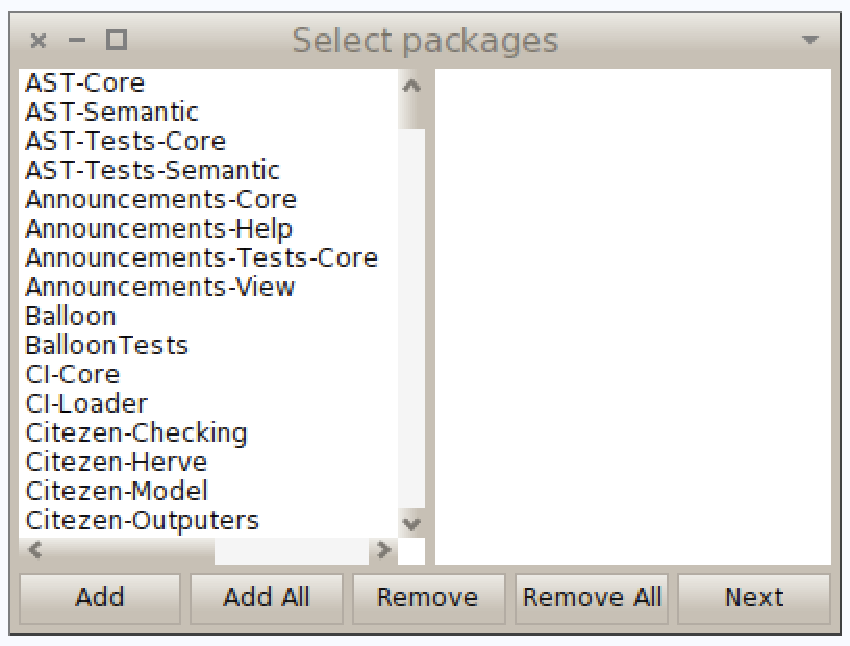
\includegraphics[width=6cm]{selectingPackage}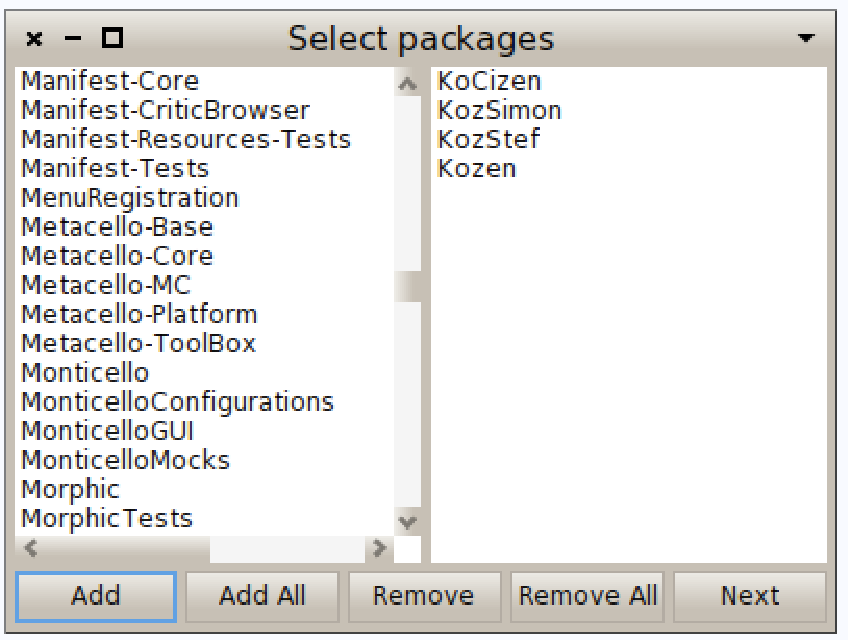
\includegraphics[width=6cm]{selectingPackage2} 
\end{figure}


\paragraph{Selecting Rules.}
Once you have selected the packages on which you want to run the rules, you can select them as shown in Figure~\ref{ruleselection}. Rules are sorted in different categories as explained in Section~\ref{existingRules}. By default running all the rules is a good idea.


\begin{figure}[h]
\centering
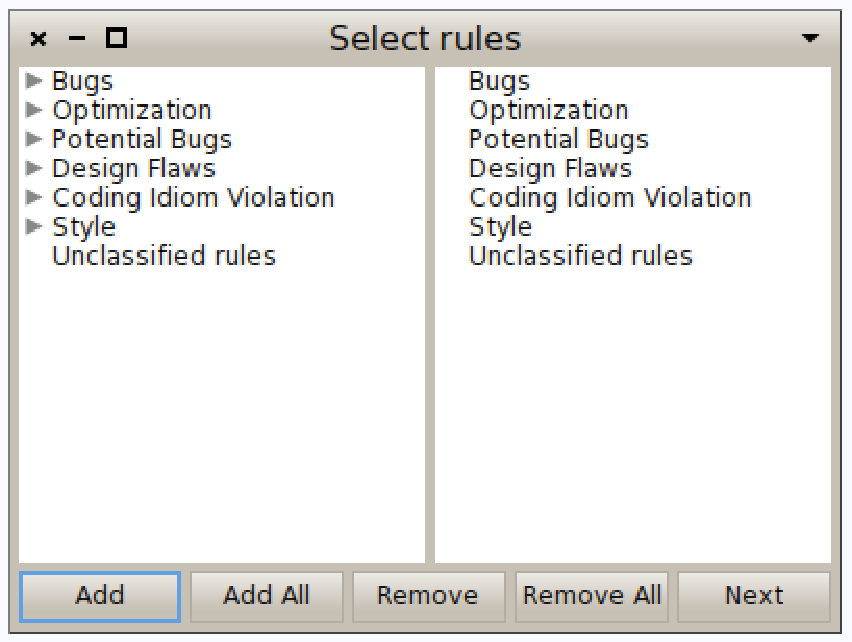
\includegraphics[width=6cm]{selectingRules}
\caption{Selecting rules. By default running all the rules is a good idea. \label{ruleselection}}
\end{figure}


\paragraph{First look at Results.} Once the rules are run you get a browser showing you the results as shown in Figure~\ref{unclassified}. 
The Critics Browser shows the results are grouped by rule kinds. 
The top level label labelled \ct{selected Rules (FP: 0, ToDo: 0, Total: 328} means the following: we got a total of 328 rule violations. Since we just started to check a new project, we did not mark any violations as false positive\footnote{A false positive is said to a violation that was detected by a tool but that was not true.}, this is why we have FP: 0, and since we did not flag violations as point to address in the future we have \ct{ToDo: 0}.


Figure~\ref{unclassified} shows that in the rules related to style

 issues, the Kozen packages got two badly classified methods. Since moving the methods to a correct method category is easy, we did it and run the rules. We obtain then the situation described by Figure~\ref{reapplying}.

The Critics Browser shows the rules on the left pane. When one rule is selected, the violations appear in the right pane. You can search by typing in the top right input field. The pane at the bottom shows either the rule description or the entity exhibiting the violation. 

\begin{figure}[h]
\centering
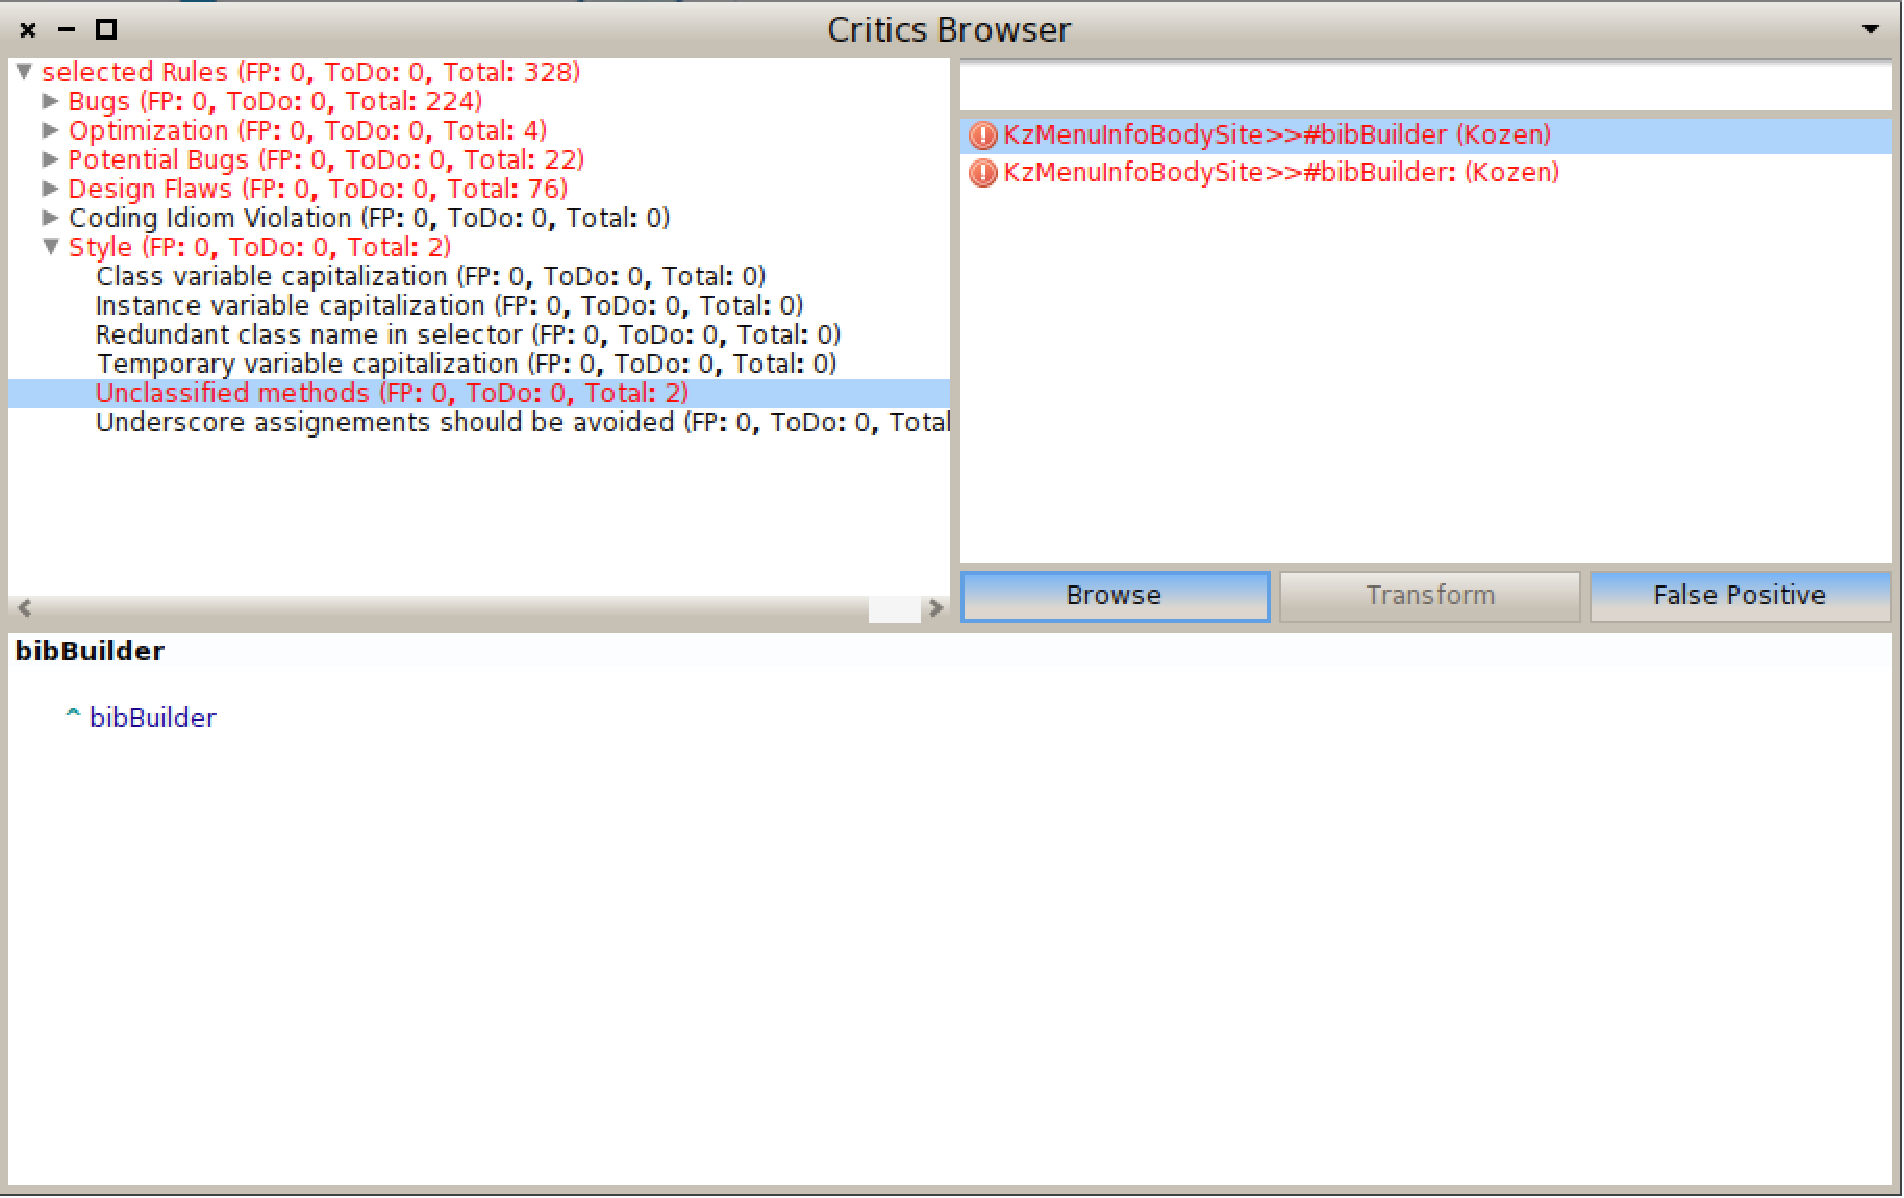
\includegraphics[width=8cm]{UnclassifiedMethods}
\caption{Browsing rule results. Two methods are not well classified in the class KzMenuInfoBodySite.\label{unclassified}}
\end{figure}


\begin{figure}[h]
\centering
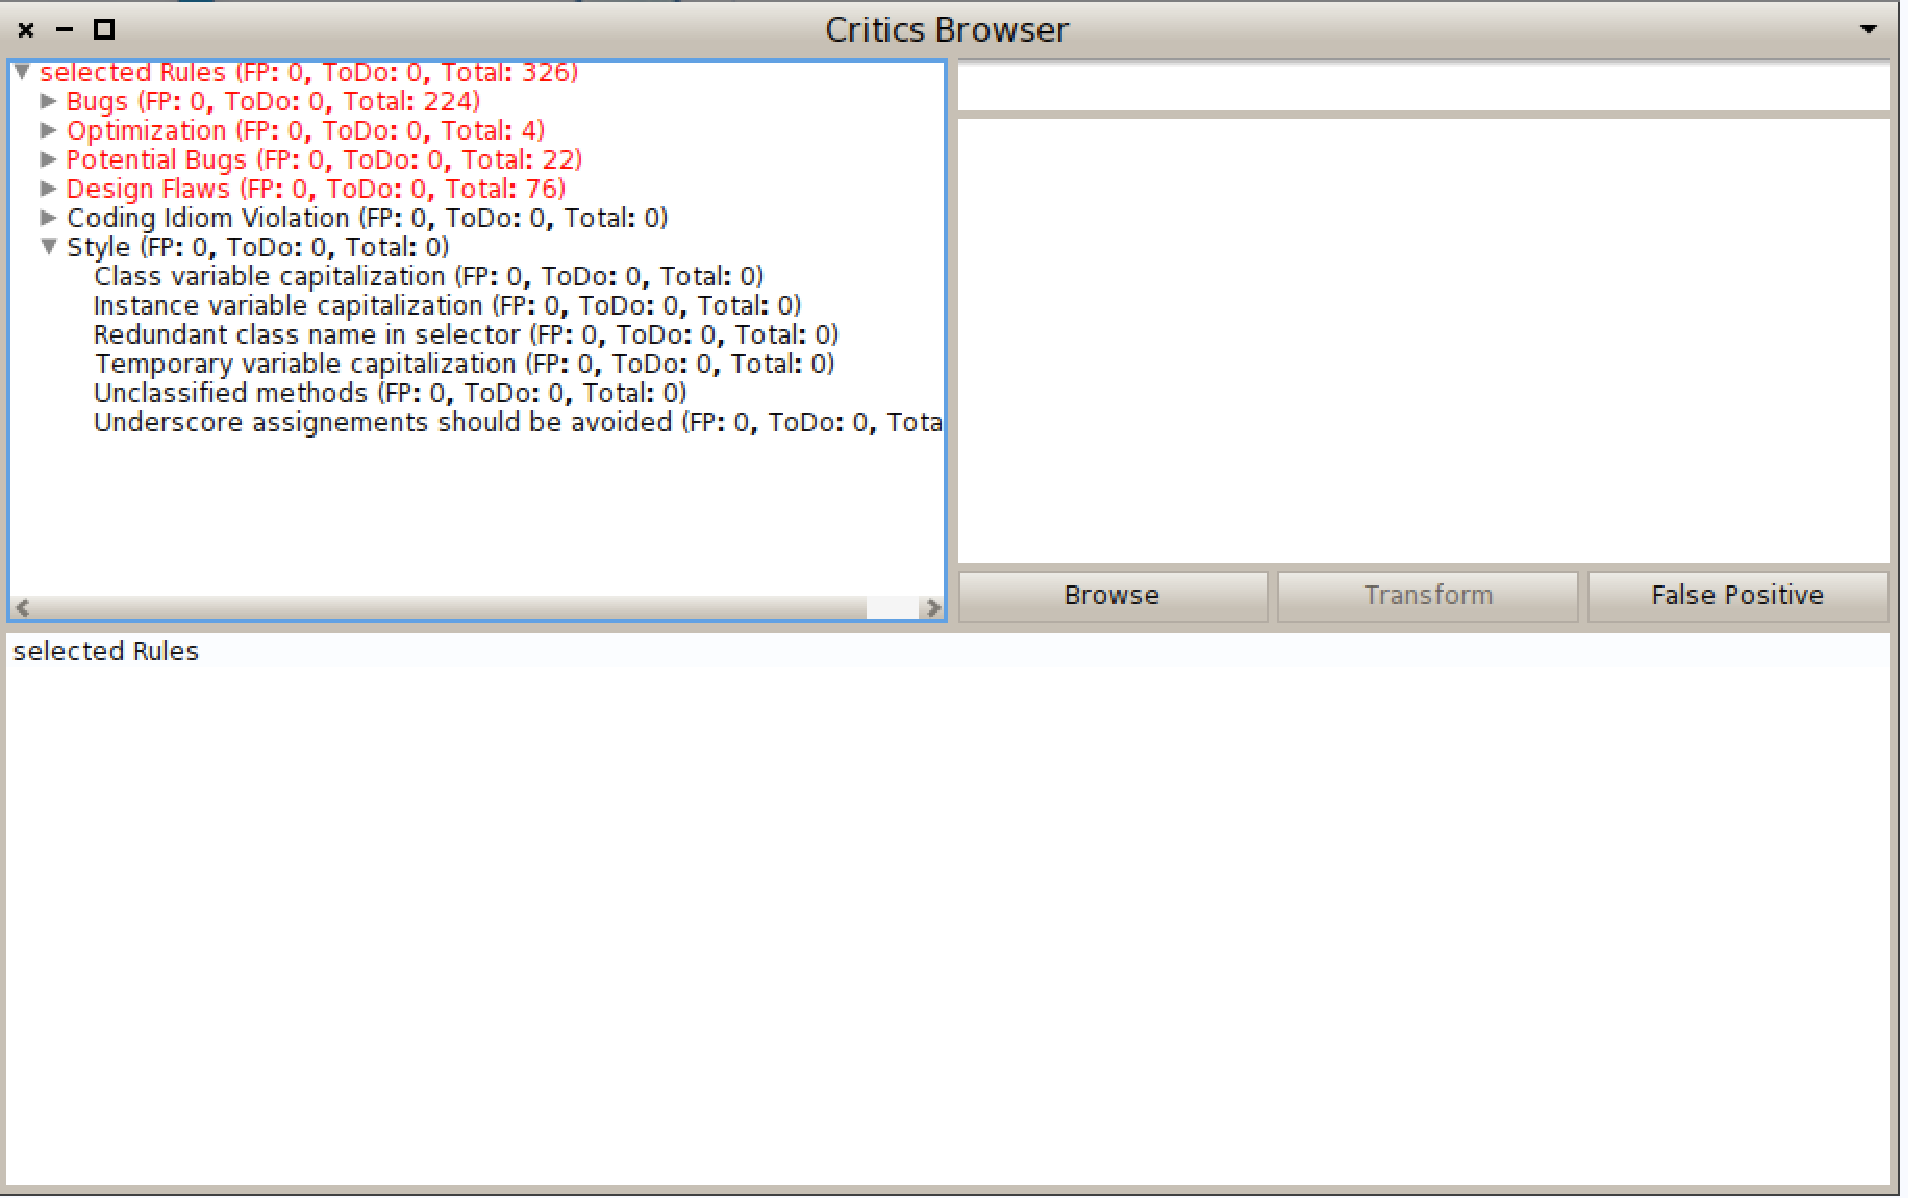
\includegraphics[width=8cm]{ReapplyingTheRulesAfterAChange}
\caption{Addressing an issue on the spot and running the rules once again\label{reapplying}}
\end{figure}





A more interesting case is the 'Bugs' category as shown by Figure~\ref{}


\paragraph{Banning a single critic.}


\begin{figure}[h]
\centering
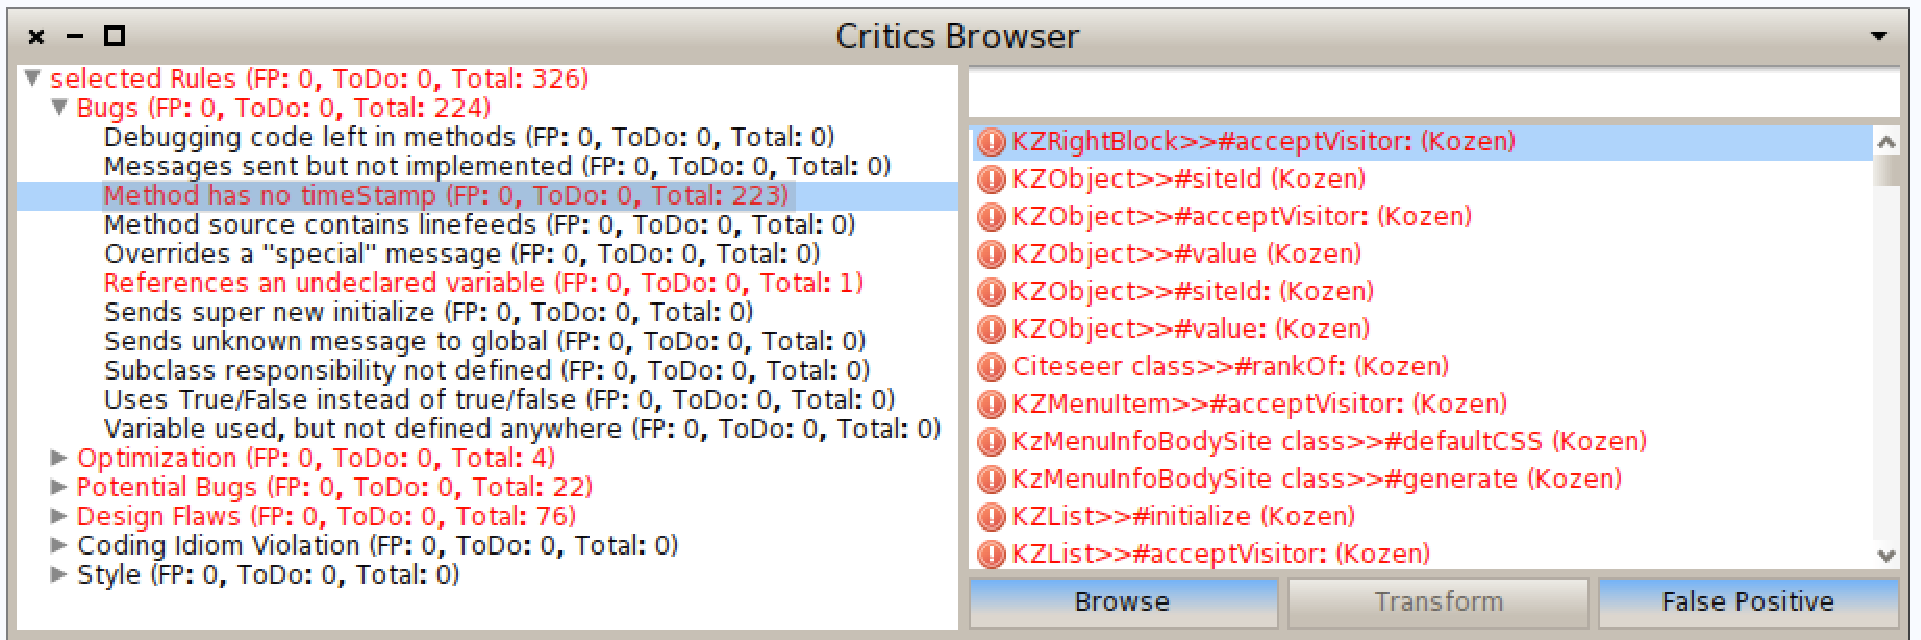
\includegraphics[width=6cm]{LookingAtBugs}
\caption{Looking at the 'Bugs' rule category.}
\end{figure}


\begin{figure}[h]
\centering
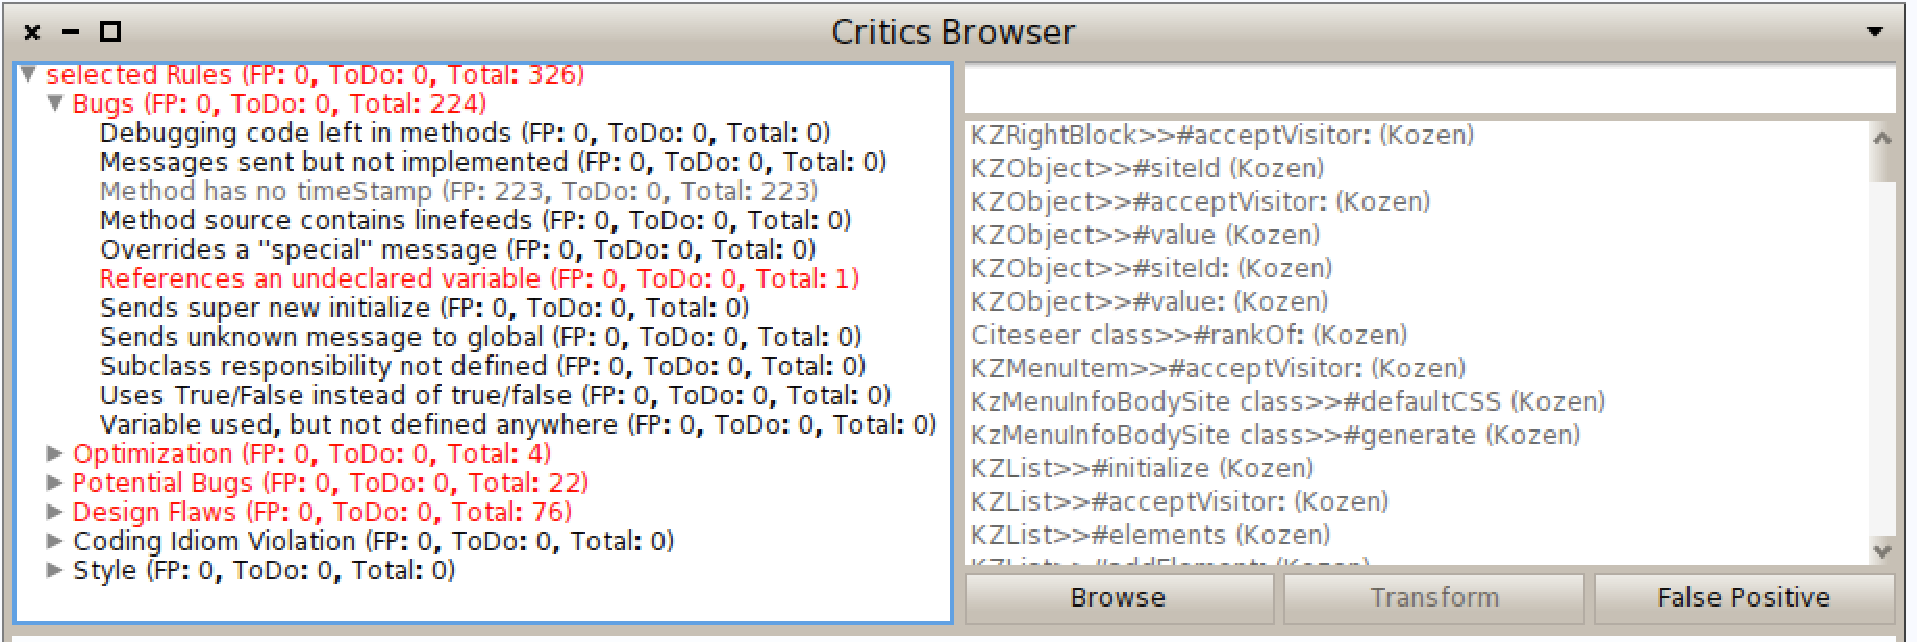
\includegraphics[width=6cm]{BanningTimeStampRules}
\caption{Banning the rule for the complete selected packages.}
\end{figure}


\paragraph{Banning a complete rule.}
If a rule is irelevante for your project, you can ban this rule for all selected packages during the rules selection step. To do this, make a right click on the rule menu and select "Ban this rule for all package". After this, all  warnings of this rule are marked as false positive (see Figure~\ref{BanningTimeStampRules}). 



\begin{figure}[h]
\centering
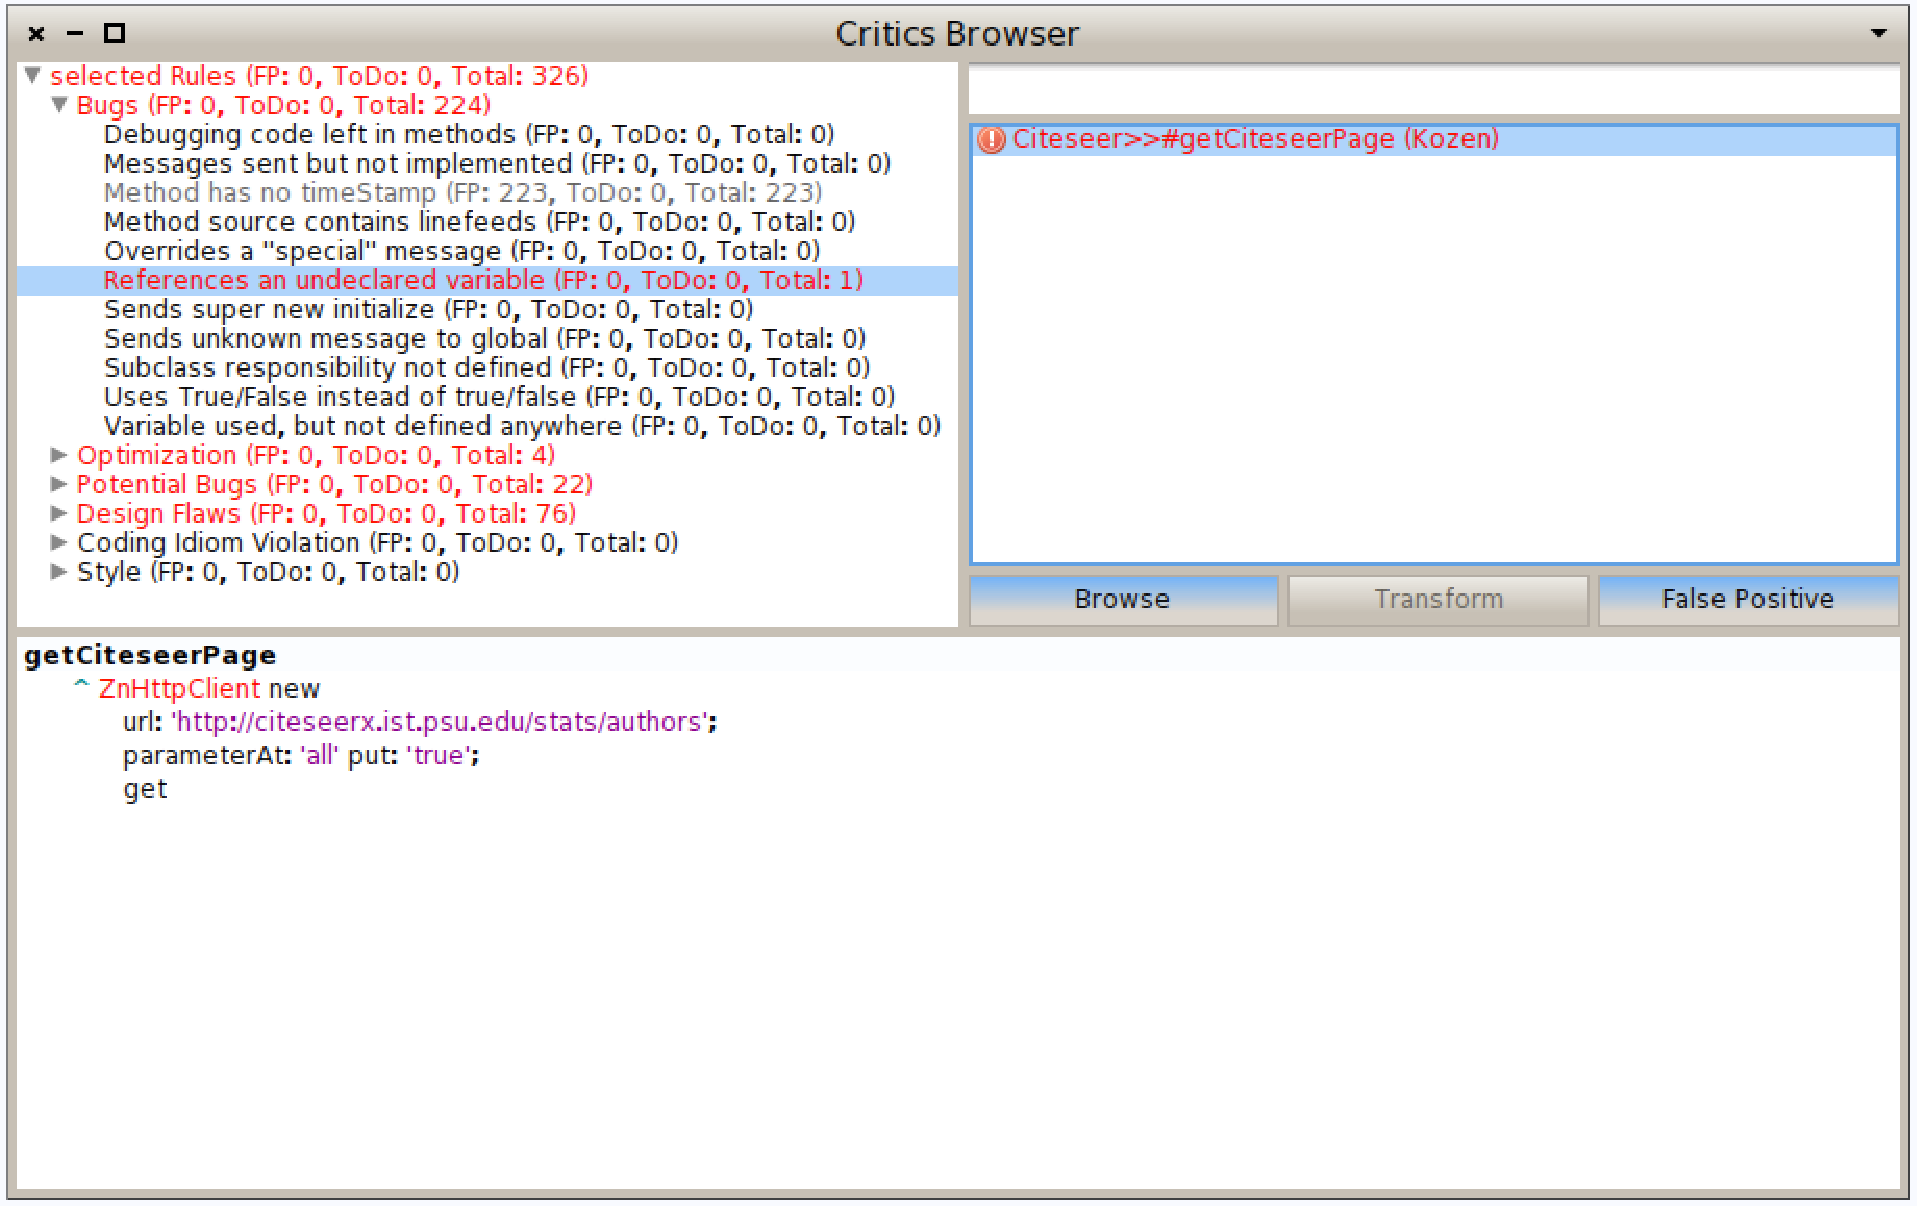
\includegraphics[width=6cm]{OneUndeclaredRefence}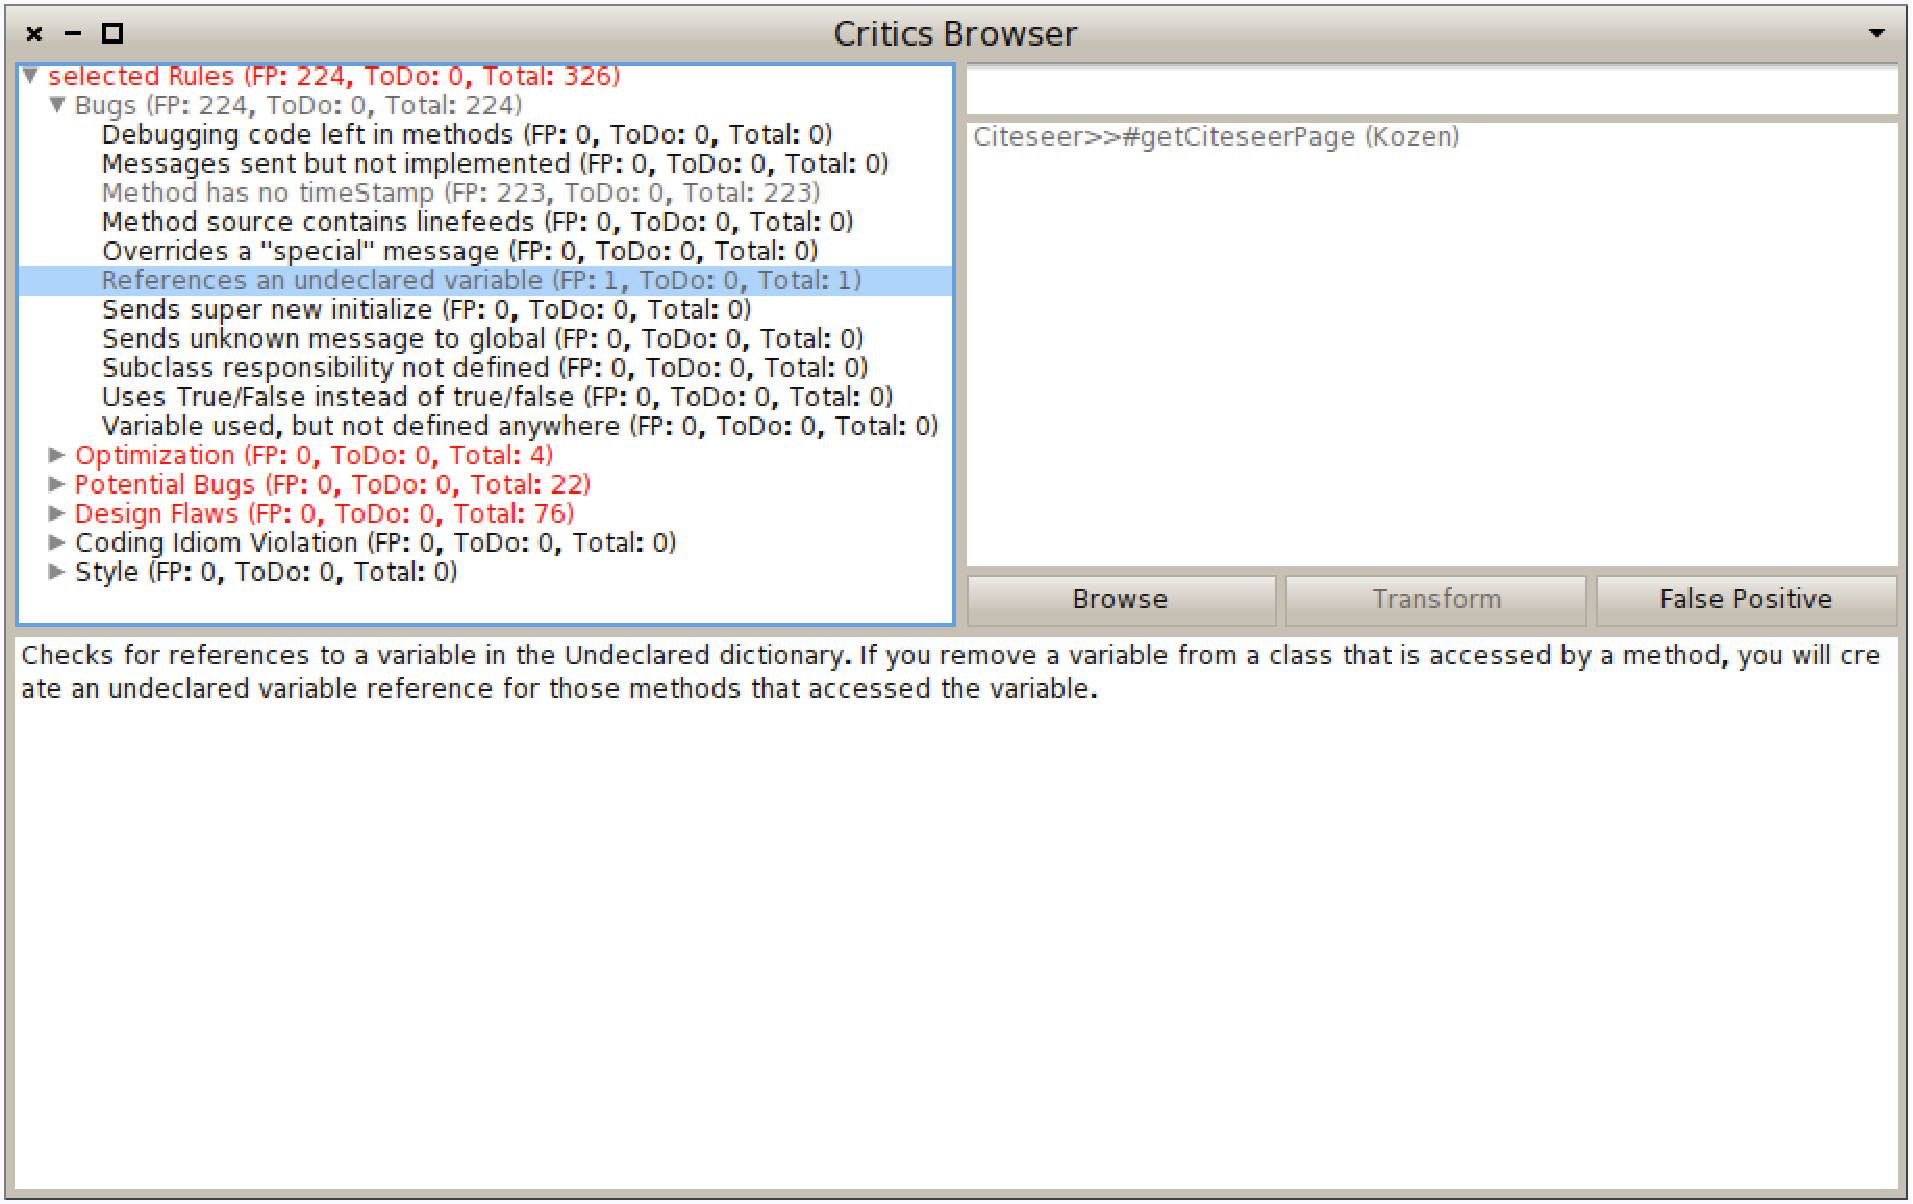
\includegraphics[width=6cm]{BanningOneViolation}
\caption{Looking at the undeclared variable bug (left) and Banning one single critic (right)}
\end{figure}




\section{Defining Your Own Rules}
SmallLint provide three different way to define rules.
\begin{itemize}
	\item Block rules use the Smalltalk reflective API. These rules can be defined at two levels: class or method.
	\item AST rules, these rules are working on ast methods. 
	\item Transformation rules, these rules performs transformation on the ast methods.
\end{itemize}

\subsection{Block Rules}

Block rules use the Smalltalk reflective API. They can be created to find methods that should be not invoked, style consistence such capitalization or variable name length, class or method size, classes not commented, variables not referenced, instance variables defined in all subclasses, among others. In resume, every thing that is possible to do using the Smalltalk reflective API can be used in a block rule. This includes access to the Smalltalk model which allows the easy navigation through classes (and their superclasses and subclasses), methods, variables, arguments, comments, invocations, etc.

These rules are created by extending the class RBBlockLintRule.
 Block rules can be defined at two levels, class or method. If the rule checks a class property or violation (eg, the presence of a class comment), this rule must implement #checkClass:. Similarly, a rule checks  a method property, the rule must implement #checkMethod:.

\paragraph{Defining Simple Rules}
Take as example the definition of a simple rule:  when a class defines #=, it also have to defines  #hash. If #hash is not defined then the instances of the class might not be able to be used in sets since equal element must have the same hash.

This rules (RBDefinesEqualNotHashRule) is a class property so we must implement #ckecClass:. Before, we implement #resultClass. This method returns the type of environement which will contains violations of the rule. For a rule at the level of class, the environment is RBClassEnvironment and RBMethodEnvironment for  a rule at the level of method.

\begin{code}{}
RBDefinesEqualNotHashRule>>#resultClass
	^ RBClassEnvironment
\end{code}

The methods #checkClass: and #checkMethod: receive in parameter the object \emph{aContext},  instance of RBSmalllintContext. This object contains information about the method/class who is currently check. For example, the method RBSmalllintContext>>#selectedClass returns the class currently check. In the case where we access to this object from #checkClass:, \emph{aContext} can provide the currently compile method chech (RBSmalllintContext>>#compiledMethod) or all messages send from this method (RBSmalllintContext>>#messages).

When the current class check violates the rule, this class is added to the enviroment which contains the set of found violation: result addClass: aContext selectedClass. 

\begin{code}{}
RBDefinesEqualNotHashRule>>#checkClass: aContext 
	((aContext selectedClass includesSelector: #=) and: 
		[ (aContext selectedClass includesSelector: #hash) not ])
			 ifTrue: [ result addClass: aContext selectedClass ]
\end{code}



Finally, the RBLintRule interface provide three methods at implement for described (#name and #longDescription) and categorize this rule (#category). The categories are \emph{Bugs}, \emph{Potential Bugs}, \emph{Optimization}, \emph{Design Flaws}, \emph{Coding Idiom Violation} and \emph{Style}. It is possible to add new category.
\begin{code}{}
RBDefinesEqualNotHashRule>>#name
	^ 'Defines = but not hash'
\end{code}

\begin{code}{}
RBDefinesEqualNotHashRule>>#longDescription
	^ 'This smell arises when a class defines #= also and not #hash. If #hash is not defined then the instances of the class might not be able to be used in sets since equal element must have the same hash.'
\end{code}

\begin{code}{}
category 
	^ 'Potential Bugs'
\end{code}

\subsection{Abstract Syntax Tree-Based Rules}

These rules are based on the Smalltalk abstract syntax tree (AST). They can be created to find assignments with no effect, weak use of the API (pieces of code can be more efficient or legible), among others. In summaty, these rules performs operation in AST nodes to find smells.

These rules are created by extending the class RBParseTreeLintRule. The last match must be defined in the initialize method.


- Example

\begin{code}{}
RBAssignmentWithoutEffectRule>>#initialize
	super initialize.
	self matcher 
		matches: '`var := `var'
		do: [ :node :answer | node ]
\end{code}

\subsection{Defining Simple Rules}

\section{Conclusion}





\ja{what are the following sections ?}

\section{Junk}

@@ here rules@@
 Pour vous en servir,
vous devez choisir les jeux de r\`egles que vous souhaitez appliquer
(dans le panneau, en haut à gauche), s\'electionner les r\`egles (panneau,
en bas à gauche), les cat\'egories (panneau du milieu), les classes
(panneau de droite), et finalement presser « Run ». Une fois que tout
est affich\'e, vous pouvez avoir acc\`es aux m\'ethodes suspectes en
cliquant sur les lignes qui d\'etaillent le r\'esultat.  Certaines
soci\'et\'es imposent aux d\'eveloppeurs d'invoquer syst\'ematiquement
SmallLint avant de d\'elivrer leur code. Notons que les r\`egles peuvent
en être particularis\'ees et qu'il est possible d'en ajouter de
nouvelles au jeu existant. La d\'efinition des r\`egles utilise la
reconnaissance de code (pattern matching) propos\'e par le RewriteTool
que nous allons maintenant \'etudier.

\section{Identification de code avec RewriteTool}

RewriteTool est un outil de r\'ecriture de code bas\'e sur la d\'efinition
de reconnaissance de formes (pattern matching), appliqu\'ee sur des
arbres de syntaxes abstraites. Une documentation plus compl\`ete est
disponible à http://st-www.cs.uiuc.edu/~brant/RefactoringBrowser/
Rewrite.html.

Il semble que Squeak ne dispose pas actuellement d'interface graphique
pour la r\'ecriture du code, mais uniquement pour identifier des
morceaux de code.


Cet outil de r\'ecriture de code est particuli\`erement utile lorsqu'on
doit transformer d'une mani\`ere r\'ep\'etitive du code. On peut repr\'esenter
dans les sch\'emas (patterns) de reconnais- sance des variables, des
listes, des instructions r\'ecursives et des litt\'eraux.

\begin{itemize}
\item	Variable. Un sch\'ema peut contenir des variables en utilisant
  le backquote ou accent grave. Ainsi, \ct{`key} repr\'esente n'importe
  quelle variable, mais pas une expression.

\item Liste. Pour repr\'esenter une expression potentiellement
  complexe, on utilise \ct{@} qui caract\'erise une liste. Ainsi, `@key
  peut repr\'esenter aussi bien une variable simple comme temp qu'une
  expression comme \ct{(aDict at: self keyForDict)}. Par exemple, | `@Temps
  | reconnaît une liste de variables temporaires. Le point . reconnaît
  une instruction dans une s\'equence de code.\ct{`@.Statements}
  reconnaît une liste d'instructions. Par exemple, foo `@message:
  \ct{`@args} reconnaît n'importe quel message envoy\'e à foo.


\item R\'ecursion. Pour que la reconnaissance s'effectue aussi à
  l'int\'erieur de l'expression, il faut doubler la quote. La seconde
  quote repr\'esente la r\'ecursion du sch\'ema cherch\'e. Ainsi,
  \ct{``@object foo} reconnaît foo, à quelque objet qu'il soit envoy\'e,
  mais observe \'egalement pour chaque reconnaissance si une
  reconnaissance est possible dans la partie repr\'esent\'ee par la
  variable \ct{``@object}.

\item	Litt\'eraux. \ct{\\#} repr\'esente les litt\'eraux ; ainsi, \ct{`\\#literal}
  reconnaît n'importe quel litt\'eral, par exemple 1, \ct{\\#()}, "unechaine"
  ou \ct{\\#unSymbol}.
\end{itemize}

\section{Des exemples d'identification de sch\'emas}

Si l'on veut identifier les expressions de type
aDict at: aKey ifAbsent: aBlock dans lesquelles les variables peuvent être des expressions compos\'ees, on \'ecrit l'expression
suivante :
\ct{``@aDict at: ``@aKey ifAbsent: ``@aBlock.}
Une telle expression identifie par exemple les expressions suivantes :

\begin{code}{}
instVarMap at: aClass name ifAbsent: [oldClass instVarNames]
deepCopier references at: argumentTarget ifAbsent: [argumentTarget]
bestGuesses at: anInstVarName ifAbsent: [self typesFor: anInstVarName]
object at: (keyArray at: selectionIndex) ifAbsent: [nil]
\end{code}

Comme l'interface en Squeak ne permet pas encore de s\'electionner les
classes sur lesquelles on veut travailler, le syst\`eme analyse les 1
934 classes et quelque 42 869 m\'ethodes qui sont disponibles dans la
distribution de base, ce qui peut sensiblement ralentir le traitement.

Voici quelques exemples d'
expressions qui pourraient être avantageusement transform\'ees :

\begin{code}{}
| `@Temps | ``@.Statements. ``@Boolean ifTrue: [^false]. ^true
| `@Temps | ``@.Statements. ^``@Boolean not
``@object not ifTrue: ``@block
``@object ifFalse: ``@block.
\end{code}


% RBParseTreeRewriter new
% 	replace: '``@aDictionary at: ``@key
% 		ifAbsent:
% 			[| `@Temps |
% 			``@.Statements.
% 			``@aDictionary at: ``@key put: ``@value]' with: '``@aDictionary at: ``@key
% 		ifAbsentPut:
% 			[| `@Temps |
% 			``@.Statements.
% 			``@value]';
% 	yourself

\begin{code}{}
rule := RBUnderscoreAssignmentRule new.
environment := BrowserEnvironment new forPackageNames: \#('PackageA'
'PackageB' ...).
SmalllintChecker runRule: rule onEnvironment: environment.
rule open
\end{code}

\begin{code}{}
ORLintBrowser
	openRule: (RBCompositeLintRule rules: (RBCompositeLintRule
rulesGroupedFor: RBSpellingRule) name: 'Spelling')
	environment: (BrowserEnvironment new forPackageNames: \#('Kernel'
'Collections-Abstract'))
\end{code}


\end{document}


%%% Local Variables: 
%%% coding: utf-8
%%% mode: latex
%%% TeX-master: Lint.tex
%%% TeX-PDF-mode: t
%%% End:
